%% ----------------------------------------------------------------
%% Thesis.tex -- MAIN FILE (the one that you compile with LaTeX)
%% ----------------------------------------------------------------

% ------------------ Set up the document -----------------------------------------------------------
%\documentclass[a4paper, 11pt, twoside, openright]{Thesis} %en a4
\documentclass[a4paper, 12pt, twoside, openright]{Thesis}  %para reducir a b5

% ------------------ Include any extra LaTeX packages required -------------------------------
\usepackage[square, numbers, comma, sort&compress]{natbib}  % Use the "Natbib" style for the references in the Bibliography
\usepackage{verbatim}         % Needed for the "comment" environment to make LaTeX comments
\usepackage{vector}           % Allows "\bvec{}" and "\buvec{}" for "blackboard" style bold vectors in maths
\usepackage[table]{xcolor}

\usepackage{parskip}          %para que haga el indent al principio de cada parrafo
\setlength{\parindent}{15pt}
\usepackage{indentfirst}      %para que ponga el indent en el primer parrafo tambien, sino no lo hace

\usepackage{lscape}           %Poner una página apaisada (util para tablas muy anchas)

\hypersetup{urlcolor=blue, colorlinks=true}  % Colours hyperlinks in blue, but this can be distracting if there are many links.


% ------------------ Abreviaciones de comandos y nuevos comandos -----------------------------------
\newcommand {\absq}[1] {\left| #1 \right|^2}

\def\la{\langle}
\def\ra{\rangle}
\def\blankpage{
\newpage
\begin{equation}
  \nonumber
\end{equation}
\newpage}
\def\ssst{\scriptscriptstyle}   %%para hacer más pequeñas algunas ecuaciones

%% Para habilitar la gamma mayuscula con blackboard style
\newcommand{\bbGamma}{{\mathpalette\makebbGamma\relax}}
\newcommand{\makebbGamma}[2]{%
  \raisebox{\depth}{\scalebox{1}[-1]{$\mathsurround=0pt#1\mathbb{L}$}}%
}

% Para doublestruck 0
\usepackage[bb=boondox]{mathalfa}

% Remove hyphen word split
% \hyphenpenalty=10000

%% ----------------- START OF THE DOCUMENT ---------------------------------------------------------
\begin{document}



\frontmatter	           % Begin Roman style (i, ii, iii, iv...) page numbering

% ------------------ Set up the Title Page ---------------------------------------------------------
\begin{titlepage}
\thispagestyle{empty} %\vspace*{0.1cm}
% \hspace{-0.3cm}\includegraphics[scale=0.25]{ehu}\hspace{0.3cm}
{\centering
\includegraphics[scale=0.25]{ehu}
}
\bigskip
{\centering \large
\par \vspace{1.5cm}

\hrule\vspace*{0.3cm}

{\LARGE \bf {Asymmetric Quantum Devices\\and Heat Transport}}

\vspace{0.3cm}\hrule \vspace{2cm}
{\LARGE \bf{Miguel \'{A}ngel Sim\'{o}n Mart\'{i}nez}}\\
\vspace{1.25cm}
{\it{Supervisors:}} \\
\vspace{0.1cm}
{\large \bf {Prof. Juan Gonzalo Muga Francisco}}\\
{\large \bf {Prof. Maria Luisa Pons Barba}}\\
% \vspace{2.2cm}
\vfill
% \begin{figure}[h]
% {\centering {
%
% }\par}
% \end{figure}
% \vspace{1.0cm}
Departamento de Qu\'{\i}mica-F\'{\i}sica\\
Facultad de Ciencia y Tecnolog\'ia\\
Universidad del Pa\'is Vasco/Euskal Herriko Unibertsitatea\\ (UPV/EHU)\\
\vspace{1.0cm}
Leioa, Abril 2021\\
} \pagebreak
\end{titlepage}
       %we use the title page document


\setstretch{1.3}        % It is better to have smaller font and larger line spacing than the other way round


% --------- Define the page headers using the FancyHdr package and set up for one-sided printing

\fancyhead{}        % Clears all page headers and footers
\rhead{\thepage}    % Sets the right side header to show the page number
\lhead{}            % Clears the left side page header
\pagestyle{fancy}   % Finally, use the "fancy" page style to implement the FancyHdr headers
\clearpage          % Declaration ended, now start a new page

% Meto una pagina en blanco
\pagestyle{empty}   % No headers or footers for the following pages
\null\vfill

\vfill\vfill\vfill\vfill\vfill\vfill\null
\clearpage          % Empty page ended, start a new page



% ------------------ The "Funny Quote Page" --------------------------------------------------------
\pagestyle{empty}  % No headers or footers for the following pages

% \null\vfill
% % Now comes the "Funny Quote", written in italics
% \textit{``It ain't much, but it`s honest work.''}
% \begin{flushright}
%   Someone who you admire or hate
% \end{flushright}
% \vfill\vfill\vfill\vfill\vfill\vfill\null
% \clearpage  % Funny Quote page ended, start a new page
%% ----------------------------------------------------------------

% ------------------ The Abstract Page -------------------------------------------------------------
%\addtotoc{Abstract}  % Add the "Abstract" page entry to the Contents
%\abstract{
%\addtocontents{toc}{\vspace{1em}}  % Add a gap in the Contents, for aesthetics
%
%The Thesis Abstract is written here (and usually kept to just this page). The page is kept centered vertically so can expand into the blank space above the title too\ldots
%
%}
%
%\clearpage  % Abstract ended, start a new page
%%% ----------------------------------------------------------------

% Meto una pagina en blanco
\pagestyle{empty}  % No headers or footers for the following pages

\null\vfill

\vfill\vfill\vfill\vfill\vfill\vfill\null
\clearpage  % Empty page ended, start a new page

\setstretch{1.3}  % Reset the line-spacing to 1.3 for body text (if it has changed)

% ------------------ The Acknowledgements page, for thanking everyone ------------------------------
\acknowledgements{
\addtocontents{toc}{\vspace{1em}}  % Add a gap in the Contents, for aesthetics

% Escribir una tesis no es tarea f\'{a}cil en general, y mucho menos en estos tiempos tan oscuros de la pandemia de COVID-19. En estos momentos m\'{a}s que nunca es vital estar rodeado de personas maravillosas que te apoyen y con las que compartir penas y alegrías. A la primera persona que tengo que nombrar en esta tesis es a ti, mi querida Cecilia. Sin ti, yo este año no habría sido capaz de seguir adelante durante los meses de encierro y teletrabajo. Has hecho que todos y cada uno de los segundos en nuestra oficina se llenen de luz y de color.

\it{Esta Tesis ha sido financiada a trav\'es de una beca predoctoral concedida por el Gobierno Vasco/Eusko Jaurlaritza}
}

\clearpage  % End of the Acknowledgements
%% ----------------------------------------------------------------

\pagestyle{fancy}  %The page style headers have been "empty" all this time, now use the "fancy" headers as defined before to bring them back


%% ----------------------------------------------------------------
\lhead{\emph{Contents}}  % Set the left side page header to "Contents"
\tableofcontents  % Write out the Table of Contents

%% ----------------------------------------------------------------
\lhead{\emph{List of Figures}}  % Set the left side page header to "List if Figures"
\listoffigures  % Write out the List of Figures

%%% ----------------------------------------------------------------
%\lhead{\emph{List of Tables}}  % Set the left side page header to "List of Tables"
%\listoftables  % Write out the List of Tables

%% ----------------------------------------------------------------
\setstretch{1.5}  % Set the line spacing to 1.5, this makes the following tables easier to read
\clearpage  % Start a new page

%% Begin the Dedication page
\setstretch{1.3}  % Return the line spacing back to 1.3
\pagestyle{empty}  % Page style needs to be empty for this page
\dedicatory{dedicatory here}

\addtocontents{toc}{\vspace{1em}}  % Add a gap in the Contents, for aesthetics
\chapter{List of publications} % Write in your own chapter title
\label{Publications}
\lhead{\emph{List of publications}} % Write in your own chapter title to set the page header
\hspace{-0.5 cm}{{\large\bf \rm I)}} {\bf The results of this Thesis are based on the following articles}
\section*{Published Articles}

\begin{enumerate}

  \item M. Pons, Y. Y. Cui, A. Ruschhaupt, {\bf M. A. Sim\'{o}n} and J. G. Muga\\
  {\it Local rectification of heat flux}\\
  \href{https://doi.org/10.1209/0295-5075/119/64001}{EPL {\bf 119}, 64001 (2017).}

  \item A. Ruschhaupt, T. Dowdall, {\bf M. A. Sim\'{o}n} and J. G. Muga\\
  {\it Asymmetric scattering by non-Hermitian potentials}\\
  \href{https://doi.org/10.1209/0295-5075/120/20001}{EPL {\bf 120}, 20001 (2017).}

  \item {\bf M. A. Sim\'{o}n}, A. Buend\'{i}a and J. G. Muga\\
  {\it Symmetries and Invariants for Non-Hermitian Hamiltonians}\\
  \href{https://doi.org/10.3390/math6070111}{Mathematics {\bf 6}, 111 (2018).}

  \item {\bf M. A. Sim\'{o}n}, A. Buend\'{i}a, A. Kiely, A. Mostafazadeh and J. G. Muga\\
  {\it $S$-matrix pole symmetries for non-Hermitian scattering Hamiltonians}\\
  \href{https://doi.org/10.1103/PhysRevA.99.052110}{Phys. Rev. A {\bf 99}, 052110 (2019).}

  \item {\bf M. A. Sim\'{o}n}, S. Mart\'{i}nez-Garaot, M. Pons and J. G. Muga\\
  {\it Asymmetric heat transport in ion crystals}\\
  \href{https://doi.org/10.1103/PhysRevE.100.032109}{Phys. Rev. E {\bf 100}, 032109 (2019).}

  \item A. Alaña, S. Mart\'{i}nez-Garaot, {\bf M. A. Sim\'{o}n} and J. G. Muga\\
  {\it Symmetries of (${N \times N}$ ) non-Hermitian Hamiltonian matrices}\\
  \href{https://doi.org/10.1088/1751-8121/ab7781}{J. Phys. A: Math. Theor. {\bf 53}, 135304 (2020).}

\end{enumerate}

\section*{Preprints}

\begin{enumerate}

  \item A. Ruschhaupt, A. Kiely, {\bf M. A. Sim\'{o}n} and J. G. Muga\\
  {\it Quantum-optical implementation of non-Hermitian potentials for asymmetric scattering}\\
  \href{https://arxiv.org/abs/2008.01702}{arXiv:2008.01702 [quant-ph] (2020)}\\
  (\href{https://journals.aps.org/pra/accepted/2f07eYb5Ibe1ea6603ef59232d2f3864c12b1a62d}{Accepted for publication in Phys. Rev. A})

  \item {\bf M. A. Sim\'{o}n}, A. Alaña, M. Pons, A. Ruiz-Garc\'{i}a and J. G. Muga\\
  {\it Heat rectification with a minimal model of two harmonic oscillators}\\
  \href{https://arxiv.org/abs/2010.10432}{arXiv:2010.10432 [cond-mat.stat-mech] (2020)}

\end{enumerate}

\vspace{1.25 cm}

\hspace{-0.65  cm}{{\large\bf \rm II)}} {\bf Other articles produced during the Thesis period}
\section*{Published  Articles not included in this Thesis}

\begin{enumerate}

  \item M. Palmero, {\bf M. A. Sim\'{o}n} and D. Poletti\\
  {\it Towards Generation of Cat States in Trapped Ions Set-Ups via FAQUAD Protocols and Dynamical Decoupling}\\
  \href{https://doi.org/10.3390/e21121207}{Entropy {\bf 21}, 1207 (2019)}

  \item {\bf M. A. Sim\'{o}n}, M. Palmero, S. Mart\'{i}nez-Garaot and J. G. Muga\\
  {\it Trapped-ion Fock-state preparation by potential deformation}\\
  \href{https://doi.org/10.1103/PhysRevResearch.2.023372}{Phys. Rev. Research {\bf 2}, 023372 (2020)}

\end{enumerate}


%% ----------------------------------------------------------------
\mainmatter	       % Begin normal, numeric (1,2,3...) page numbering
\pagestyle{fancy}  % Return the page headers back to the "fancy" style

% --------------------------------------------------------------------------------------------------
% ------------------ Include the chapters of the thesis, as separate files -------------------------
% --------------------------------------------------------------------------------------------------

\addtocontents{toc}{\vspace{0.6em}}

% ------------ INTRODUCTION ------------------------------------------------------------------------
\part*{Introduction}
\addcontentsline{toc}{part}{Introduction}
%!TEX root = ../Thesis.tex

% \chapter*{Introduction} % Write in your own chapter title
\label{Introduction}
\lhead{\emph{Introduction}} % Write in your own chapter title to set the page header

Devices that control the flow of energy or matter play a prominent role in technology. A key device is the rectifier, which allows currents only one way. A rectifier behaves like a corridor with a trap door that can be opened from left to right but is closed otherwise. The most notable of such devices is the electric diode, which is a vital part of computers, digital devices, and AC/DC current conversion systems. Without the diode most of the technology that we have today would not exist.

The electric diode is an electrical component that allows electrical current to flow asymmetrically with respect to the sign of the potential difference that is applied to it. Typically, a diode is composed by the union of a $p$-semiconductor with an $n$-semiconductor. When a forward-bias potential $\Delta V$ is applied to the $p$-$n$ junction (by connecting the positive pole of a battery to the $p$-semiconductor), electrical current will flow through the diode. However, the $p$-$n$ junction acts as an electrical insulator if a reversed-bias potential $-\Delta V$ is applied.

Motivated by the technological impact of the diode, analogous devices have been developed in other physical scenarios, like optics. An optical equivalent to the diode is the optical isolator, which is used to allow one-way light propagation \cite{Saleh1991}. This device is based on the non-reciprocal rotation of the polarization direction of polarized light in materials that are in a magnetic field, known as Faraday Rotation (see ref. \cite{Yariv1984}). The optical isolator is a critical component in optical devices to protect delicate light sources from back-propagating light.

At this point we can see that a common ingredient between devices which show a diode-like behaviour is some kind of internal structural asymmetry. In the electric diode this asymmetry comes from the asymmetric distribution of charge carriers: electrons in the $n$-side, and holes in the $p$-side. In the optical isolator the orientation of the magnetic field breaks the symmetry of the system.

This Thesis is devoted to explore the physics and possible designs of devices that implement a \textit{diodic} or rectifying mechanism for an asymmetric transport of matter or energy. The Thesis
is divided into two parts: In part \ref{partI}, I look for asymmetric particle scattering of 1-dimensional quantum potentials and in part \ref{partII}, I will study thermal rectification in chains of oscillators. There follows an introduction to these two parts.


\section*{Introduction to part I: non-Hermitian systems and asymmetric scattering}

The current interest to develop new quantum technologies is boosting applied
and fundamental research on quantum phenomena and systems with potential
applications in logic circuits, metrology, communications or sensors. Robust basic devices performing elementary operations are needed to perform complex tasks when combined in a circuit. With the development of new quantum technologies in mind, the objective of this part is to design 1-dimensional scattering potentials for a quantum, spinless particle of mass $m$ that lead to transmission and reflection coefficients (squared modulus of the amplitudes) which differ for wave packets coming from the left or the right.

To find an asymmetric scattering behavior, I will use non-Hermitian and non-local potentials \cite{Muga2004,Mostafazadeh2018}. Although non-local and non-Hermitian potentials might seem uncommom and extraordinary in quantum physics to some, they appear naturally when applying partitioning techniques to describe the effective interactions in a subspace of a larger system with a Hermitian Hamiltonian by projection \cite{Feshbach1958,Ruschhaupt2004,Muga2004}. Non-Hermitian Hamiltonians representing effective interactions have a long history in nuclear, atomic, and molecular physics, and have become common in optics, where wave equations in waveguides could simulate the Schr\"odinger equation \cite{Ruschhaupt2005,Longhi2017a,Konotop2016}. Non-Hermitian Hamiltonians can also be set phenomenologically, e.g. to describe dissipation \cite{Ruschhaupt2005}. Recently there has been a lot of interest in non-Hermitian Hamiltonians \cite{Nixon2016,Nixon2016a,Chen2017,Ruschhaupt2017,Simon2018,Simon2019a,Alana2020,Bernard2002,Kawabata2019}, in particular, the ones having parity-time (PT) symmetry \cite{Bender1998,Znojil2015} because of their spectral properties and useful applications, mostly in optics  \cite{Longhi2017a,Konotop2016,Longhi2014}. However, I shall emphasize that symmetries different from PT exist and are necessary to produce certain forms of asymmetric scattering.

The contents of this part of the Thesis will be organized as follows. In chapter \ref{Chapter1}, I will use non-Hermitian and non-local potentials to design potentials with asymmetric scattering coefficients for left/right incidence. Symmetries for non-Hermitian Hamiltonians will be generalized using the concept of pseudohermiticity \cite{Mostafazadeh2002} and used to derive useful selection rules for the transmission and reflection coefficients. In chapter \ref{Chapter2}, I will derive a set of properties of the eigenvalues of scattering potentials that extend previous results for discrete non-Hermitian Hamiltonians by using the generalized symmetries. In chapter \ref{Chapter3}, I will present a possible physical realization for asymmetric scattering Hamiltonians in a quantum optics setup.


\section*{Introduction to part II: Heat rectification in mesoscopic systems}

Radiation, heat and electricity are prominent mechanisms of energy transport. In particular, the two last mechanisms play a dominant role in technology. Modern information processing rests on electronic devices like the diode and the transistor. However, there is not an analogous technology to control heat currents driven by phonons. An explanation could be that phonons are more difficult to control than electrons since (contrary to them) they do not have mass or electrical charge \cite{Li2012}. However, it would be interesting to explore the design of \textit{phononic} devices due to the richness of different physical mechanisms that mediate heat transport. The thermal rectifier, or thermal diode, would be a primary building block to develop \textit{phononics} \cite{Li2012}. In this part I study thermal rectification in chains of oscillators with the design of a thermal diode in mind.

Thermal rectification is the physical phenomenon, analogous to electrical current rectification in diodes, in which heat current through a device or medium (the thermal diode or rectifier) is not symmetric with respect to the exchange of the bath temperatures at the boundaries. It was  first observed in 1936 by Starr in a junction between copper and cuprous oxide \cite{Starr1936}. The theoretical work started much later using as rectifiers simple anharmonic chain models
with different segments \cite{Terraneo2002,Li2004}. These papers sparked much research that continues to this day. Research on thermal rectification has gained a lot of attention in recent years as a key ingredient to build prospective devices to control heat flows similarly to electrical currents \cite{Roberts2011,Li2012}. There are  proposals to engineer thermal logic circuits \cite{Ye2017} in which information, stored in thermal memories \cite{Wang2008}, would be processed in thermal gates \cite{Wang2007}. Such thermal gates, as their electronic counterparts,  would require thermal diodes and thermal transistors to operate \cite{Li2006,Joulain2016}.
Heat rectifying devices would also be quite useful in nanoelectronic circuits, letting delicate components dissipate heat while being protected from external heat sources \cite{Roberts2011}.

Most work on thermal diodes has been theoretical with only a few experiments (see refs. \cite{Chang2006,Kobayashi2009,Leitner2013,Elzouka2017}).
A relevant attempt to build a thermal rectifier was based on a graded structure made of carbon and boron nitride nanotubes that transports heat between a pair of heating/sensing circuits \cite{Chang2006}. One of the ends of the nanotube is covered with a deposition of another material, which makes the heat flow better from the covered end to the uncovered end. However, rectifications were small, with rectification factors around $7\%$.

Much of the theoretical effort in thermal rectification research has been aimed at improving the rectification factors and the features of the rectifiers. The first approach to designing thermal diodes consisted in using chains of oscillators segmented into two or more regions with different properties \cite{Terraneo2002,Li2004,Li2008,Hu2006}, which is reminiscent of the idea of the $p$-$n$ junction in electric diodes. However, it was soon noticed that the performance of segmented rectifiers was very sensitive to the size of the device, \textit{i.e.}, rectification decreases when increasing the length of the rectifier \cite{Hu2006}. To overcome this limitation two ideas were proposed. The first one consisted in using graded rather than segmented chains, \textit{i.e.}, chains where some physical property varies continuously along the site position such as the mass of particles in the chain \cite{Wang2012,Chen2015,Romero-Bastida2017,Yang2007,Romero-Bastida2013,Dettori2016,Pereira2010,Pereira2011,Avila2013}. The second one consisted in using chains with long-range interactions (LRI), such that all the elements in the chain interact with all the rest \cite{Chen2015,Bagchi2017,Pereira2013}. The rationale behind these proposals was that in a graded system, new asymmetric rectifying channels are created, while the long-range interactions create
also new transport channels, avoiding the usual decay of heat flow with size \cite{Chen2015}. Besides a stronger rectification power, LRI graded chains are expected to have better heat conductivity than segmented ones. This is an important point for technological applications, because devices with high rectification factors are not useful if the currents that flow through them are very small.

Another main focus of the theoretical research in thermal rectification is the search for the fundamental factors that contribute to the emergence of rectification. Historically, the crucial elements for having rectification have been the presence of some structural asymmetry in the system and of non-linear (anharmonic) forces \cite{Zeng2008,Katz2016,Li2008,Hu2006,Benenti2016,Li2012,Segal2005,Segal2005b}, which lead to a temperature dependence of the phonon bands or power spectral densities. A match or mismatch of the phonon bands of neighboring parts of the chain implies corresponding good or bad conduction so the
sign of the temperature bias may affect the conduction and lead to rectification when the spectra of the parts are affected differently by the bias reversal. However, more recent research pointed out that anharmonicity is not a necessary condition for an asymmetric match/mismatch and therefore for rectification \cite{Pereira2017}. Rectification also occurs in simple (minimalistic) harmonic models that incorporate some structural asymmetry and temperature-dependence of the model parameters \cite{Pereira2017}. This dependence may indeed result from an underlying, more intricate  anharmonic system by linearization of the stochastic dynamics \cite{Pereira2017,Pereira2019}, or it may have a different origin \cite{Simon2019}.


The contents of this part of the Thesis will be organized as follows. In chapter \ref{Chapter4}, I present a model of a thermal rectifier that relies on a localized impurity in the middle of a chain of atoms. In chapter \ref{Chapter5}, a proposal for a thermal rectifer in a chain of trapped ions with a graded frequency distribution is presented. Finally, in chapter \ref{Chapter6}, I study heat transport in a solvable model of two connected oscillators to explore the origin an optimization of thermal rectification.
 %Introduction

% ------------ PART I: NH-Devices ------------------------------------------------------------------
\part{Non-hermitian systems and asymmetric scattering}
%!TEX root = ../Thesis.tex
%IntroductionPartI

\chapter*{Introduction to Part I}
\addcontentsline{toc}{chapter}{Introduction to Part I}
\label{IntroductionPartI}
\lhead{Introduction to Part I} % Write in your own chapter title to set the page header

The current interest to develop new quantum technologies is boosting applied
and fundamental research on quantum phenomena and systems with potential
applications in logic circuits, metrology, communications or sensors. Robust basic
devices performing elementary operations are needed to perform complex tasks
when combined in a circuit. With the goal of increasing the knwoledge in quantum technologies and making proposals for new applications of quantum physics, in this chapter I will approach the design of devices that control the flow of quantum particles in an asymmetric way. In order to achieve this I will investigate the properties of potentials with asymmetric
transmission or reflection for a quantum, spinless particle of mass $m$ satisfying a one-dimensional (1D) Schr\"odinger equation.

We propose six different types of asymmetric devices, see fig. \ref{cases}. The six types of devices are classified according to the transmission and reflection coefficients of the scattering potentials, which in the ideal case would take only values of 0 or 1. For example, the device in fig. \ref{cases}(a), called \textit{One-way mirror} ($\cal{TR/A}$) reflects back and transmits incoming wave packets with the same intensity for left incidence, whereas all the wave packets coming from the right are completely absorbed. In fig. \ref{cases}(c) the \textit{One-Way T-filter} ($\cal{T/A}$) would be the equivalent to a diode, since it transmits all the wave packet for left incidence while it behaves as an insulator for right incidence.

\begin{figure}
  \center
  \includegraphics[width = 0.5\linewidth]{Figures/PotentialCasesPT.pdf}
  \caption{Devices with asymmetric scattering (limited to scattering coefficients being 0 or 1).  The dashed and continuous lines represent respectively zero or one
  for the moduli of the scattering amplitudes; the bended lines are for reflection amplitudes, and the straight lines for transmission:
  (a) One-way mirror ($\cal{TR/A}$); (b) One-way barrier ($\cal{T/R}$); (c) One-Way T-filter ($\cal{T/A}$);
  (d) Mirror \& 1-way transmitter ($\cal{TR/R}$); (e) One-way R-filter ($\cal{R/A}$); (f) Transparent, one-way
  reflector ($\cal{TR/T}$).
  The letter codes summarize the effect of left and right incidence, separated by a  slash ``$/$''.
  ${\cal T}$ or ${\cal R}$ on one side of the slash indicate a unit
  transmission or reflection coefficient
  for  incidence from that side, whereas the absence of one or the other letter corresponds to zero coefficients.
  An ${\cal A}$ denotes ``full absorption'', i.e., both moduli of reflection and transmission amplitudes are zero for incidence from one side.
  For example,  $\cal{TR/A}$ means unit modulus transmission
  and reflection from the left and total absorption from the right.
  \label{cases}}
\end{figure}

As we shall see in the following chapters, the asymmetric devices in fig. \ref{cases} cannot be constructed with Hermitian Hamiltonians/potentials \cite{Muga2004,Mostafazadeh2018}. Some of them even require the potential not being local. Thus  non-local, and non-Hermitian potentials are needed to implement a rich set of scattering asymmetries, and in particular asymmetric transmission.

Although nonlocal and nonhermitian potentials may seem uncommom and extraordinary in quantum physics, they appear naturally when applying partitioning techniques to describe the effective interactions in a subspace of a larger system with a Hermitian Hamiltonian by projection \cite{Feshbach1958,Ruschhaupt2004,Muga2004}. Non-Hermitian (NH) Hamiltonians representing effective interactions have a long history in nuclear, atomic, and molecular physics, and have become common in optics, where wave equations in waveguides could simulate  Schr\"odinger equations \cite{Ruschhaupt2005,Longhi2017a,Konotop2016}. NH Hamiltonians can also be set phenomenologically, e.g. to describe dissipation \cite{Ruschhaupt2005}.

Recently there has also been a lot of interest in Non-Hermitian Hamiltonians \cite{Nixon2016,Nixon2016a,Chen2017,Ruschhaupt2017,Simon2018,Simon2019a,Alana2020,Bernard2002,Kawabata2019}. In particular, the ones having parity-time (PT) symmetry \cite{Bender1998,Znojil2015} because of their spectral properties and useful applications, mostly in optics  \cite{Longhi2017a,Konotop2016,Longhi2014}. As happens with Hermitian Hamiltonians, symmetry operations on NH Hamiltonians can be systematized into group structures \cite{Ruschhaupt2017,Simon2019a,Alana2020}. In particular for
1D scattering potentials, the different Hamiltonian symmetries imply
selection rules for asymmetric transmission and reflection \cite{Ruschhaupt2017,Simon2019a} that will pose limitations to the design of the asymmetric devices in fig. \ref{cases}.
%

The contents of this part of the thesis will be organized as follows. In chapter \ref{Chapter1} I will give a brief introduction to the theory of scattering in one dimension by non-hermitian potentials. Next, I will describe the set of asymmetric devices and the different selection rules imposed by the set of symmetries formed by parity, time-reversal and PT. In chapter \ref{Chapter2} I will further investigate an extended symmetry group on the Hamiltonians that will have interesting consequences on the eigenvalues. In chapter \ref{Chapter3} I discuss possible physical implementations of non-local and non-hermitian potentials with 3-level atoms interacting with laser fields.

%!TEX root = ../Thesis.tex
%Chapter 1

\chapter{Asymmetric scattering by non hermitian potentials}
\label{Chapter1}
\lhead{Chapter 1. \emph{Asymmetric scattering by non hermitian potentials}}
%
\null\vfill
\textit{``You must unlearn what you have learned.''}
\begin{flushright}
  {\bf Master Yoda}\\
  The Empire Strikes Back
\end{flushright}
\vfill\null

The scattering of quantum particles by non hermitian (generally non-local)  potentials in one dimension may result in asymmetric transmission and/or reflection for left and right incidence.
Extending the concept of symmetry for non hermitian potentials, eight generalized symmetries based on the discrete  Klein's four-group
(formed by parity, time reversal, their product, and identity) are found. Together with generalized unitarity relations they determine selection rules for the possible and/or forbidden scattering asymmetries. Six basic device types are identified when the scattering coefficients adopt zero/one values, and transmission and/or reflection are asymmetric. They can pictorically be described as a
one-way mirror, a one-way barrier (a Maxwell  pressure demon), one-way (transmission or reflection) filters, a mirror with unidirectional transmission, and a transparent, one-way reflector. In this chapter I present potentials that have been designed to implement some of these devices and also demonstrate that the  behavior of the scattering
coefficients can be extended to a broad range of incident momenta.
%
\newpage
%

\section{Introduction\label{sec:chapter1_Introduction}}

In this chapter I study the properties of potentials with asymmetric transmission or reflection for a quantum, spinless particle of mass $m$ satisfying a one-dimensional (1D) Schr\"{o}dinger equation. I propose six types of asymmetric devices according to the asymmetries of the transmission/reflection coefficients, see fig. \ref{cases}. Non hermitian and non local potentials will be necessary to construct this kind of devices, therefore an important part of this chapter will consist in studying their properties. In particular their behaviour w.r. to symmetries such as parity, time-reversal and PT. Symmetries can be used, analogously to their standard application in atomic physics to determine selection rules for allowed/forbidden transitions, to predict whether a certain potential may or may not lead to asymmetric scattering. The concept of symmetry, however, must be generalized when dealing with non hermitian potentials.

The theory in this chapter is worked out for particles and the Schr\"odinger equation but it is clearly of relevance for optical devices
due to the much exploited analogies and connections between Maxwell's equations and the Schr\"odinger equation,
which were used, e.g., to propose  the realization of PT-symmetric potentials in optics \cite{Ruschhaupt2005}.

I will first start by introducing the formalism of quantum scattering in one dimension by non-hermitian potentials and the concept of left/right eigenvectors and biorthogonal partners, which will be fundamental to understand the rest of the chapter. It will be followed by the definition of generalized symmetries for non hermitian Hamitonians, that will be studied in detail for the 4-group composed by parity, time reversal, their product, and identity. I then derive the selection rules for the scattering coefficients corresponding to the different symmetries. Finally I will describe the types of asymmetric devices that can be built and how the different symmetries affect them.


\section{non hermitian scattering in 1 dimension \label{sec:chapter1_ScattFormalism}}

In this section I will put together the minimum set of ideas and tools needed to describe scattering in 1 dimension. The ideas in the section can be found with more detail in \cite{Muga2004}, which generalizes the results in the celebrated book by Taylor \cite{Taylor1972} to non hermitian hamiltonians. In scattering theory one deals with the usual Hamiltonian for a particle of mass $m$ subjected to the action of a potential $V$
%
\begin{equation}
  H =  H_0 + V,
\end{equation}
%
where $H_0=\frac{P^2}{2m}$ is the kinetic energy operator, with $P$ the momentum operator. The potential $V$ is not assumed to be either hermitian or local. Before continuing, I shall clarify these two statements. A linear operator $\mathcal{O}$ is hermitian, or also self-adjoint, if it is equal to its adjoint operator $\mathcal{O}^\dagger$. The definition of the adjoint of a linear operator is given by the equation
%
\begin{equation}
  \braket{\phi}{\mathcal{O}\psi} = \braket{\mathcal{O}^\dagger\phi}{\psi}\quad\forall\ket{\psi},\,\ket{\phi}\in\mathcal{H},
  \label{eq:chapter1_adjointLinearOperators}
\end{equation}
%
Where $\mathcal{H}$ is the Hilbert space of the particle. A potential $V$ with a diagonal representation in the position basis $\{\ket{x}\}$ of the particle's Hilbert space is said to be local
%
\begin{equation}
  \mel{x}{V_{local}}{x'} = \delta(x-x')V(x'),
  \label{eq:chapter1_localPotential}
\end{equation}
%
whereas a non local potential has off-diagonal elements
%
\begin{equation}
  \mel{x}{V_{non local}}{x'} = V(x,x').
  \label{eq:chapter1_nonLocalPotential}
\end{equation}
%
The potentials that we study are then non-diagonal and satisfy $V \neq V^\dagger$, therefore, the Hamiltonians will also be non-hermitian, $H \neq H^\dagger$.

Scattering theory tries to answer the following question: given an input (incident) wave packet $\ket{\psi_{in}}$, in which output (outcoming) wave packet $\ket{\psi_{out}}$ transforms into after interacting with the potential? Another way of formulating the same question is: given an incoming state with a momentum $p$, what are the probability amplitudes of the state being reflected and transmited elastically (with the same energy)? To answer these questions the scattering theory brings in the scattering states, eigenstates of the Hamiltonian which belong to the continuum part of the spectrum, \textit{i.e.}, eigenstates of the Hamiltonian which are not bounded to a finite portion of the space and behave asymptotically as plane waves far from the range of action of the potential. The scattering states represent incoming waves with momentum $p$ and energy $E_p = \frac{p^2}{2m}>0$ that are partially reflected and transmitted by the potential. For a plane wave with momentum $p>0$ incoming from the left which is transmited to the right and reflected back, the asymptotic scattering state is $\ket{p^+}$
%
\begin{equation}
  \braket{x}{p^+} =
  \begin{cases}
    \braket{x}{p} + R^l(p)\braket{x}{-p} \quad &\text{if}\; x \to -\infty
    \\
    T^l(p) \braket{x}{p} \quad &\text{if}\; x \to \infty
  \end{cases},
  \label{eq:chapter1_leftState}
\end{equation}
%
where $T^l(p)$ and $R^l(p)$ are the transmission and reflection coefficients for left incidence. $\braket{x}{p} = \frac{1}{ \sqrt{2\pi\hbar} } e^{-i p x /\hbar} $ is the unnormalized momentum eigenstate. Similarly, for a plane wave incoming from the right with momentum $-p \;(p>0)$ which is transmited to the left and reflected back, the scattering state is $\ket{-p^+}$
%
\begin{equation}
  \braket{x}{-p^+} =
  \begin{cases}
    T^r(p) \braket{x}{-p} \quad &\text{if}\; x \to -\infty
    \\
    \braket{x}{-p} + R^r(p)\braket{x}{p} \quad &\text{if}\; x \to \infty
  \end{cases},
  \label{eq:chapter1_rightState}
\end{equation}
%
where $T^r(p)$ and $R^r(p)$ are the transmission and reflection coefficients for right incidence. %Additionally to the scattering states in eqs. \eqref{eq:chapter1_leftState} and \eqref{eq:chapter1_rightState} it is possible to take a negative value of the momentum $p<0$ that will give formally correct scattering eigenstates $\ket{\pm p^-}$ of energy $E_p$ that are, however more difficult to interpret. Roughly, they can be interpreted as a time-reversed scattering process since they consist in a superpositions of 2 plane waves, one coming from the left and the other one from the right which after interacting with the potential recombine into an outgoing plane wave.
We shall see that in general $T^l\neq T^r$, $R^l\neq R^r$ for Hamiltonians that are nonhermitian and non-local. Taking the adjoint of the Hamiltonian $H^\dagger = \frac{P^2}{2m} + V^\dagger$, we can also obtain the scattering states and scattering coefficients (reflection and transmission) for left and right incidence for the adjoint: $\widehat{T}^l(p)$, $\widehat{R}^l(p)$, $\widehat{T}^r(p)$ and $\widehat{R}^r(p)$. In the rest of this thesis I will use the convention that hatted variables $\widehat{...}$ will refer to the adjoint hamiltonian $H^\dagger$. In the following, all the results I write down for $H$ can be obtained also for $H^\dagger$ by making the change $H \to H^\dagger$.

Scattering theory provides the method to obtain the scattering amplitudes through the transition operator $T_{op}(z)$, which is defined as
%
\begin{equation}
T_{op}(z) = V + VG(z)V,
\label{eq:chapter1_transitionOperator_definition}
\end{equation}
%
with $G(z) = (z-H)^{-1}$ being the Green's operator. In \cite{Muga2004} the transition operator is used to obtain the scattering eigenstates as
%
\begin{equation}
  \ket{\pm p^+} =  \ket{\pm p} + \lim_{ \varepsilon\to 0^+ } G^0(E_p + i\varepsilon)T_{op}(E_p + i\varepsilon)\ket{\pm p}\quad (p>0),
  \label{eq:chapter1_scatteringStateFormal}
\end{equation}
%
where $G^0(z) = (z-H_0)^{-1}$ is the Green's operator of the free propagation Hamiltonian $H_0$. Now, to obtain the scattering amplitudes of reflection and transmission, one has to take the limits of $\braket{x}{\pm p^+}$, where $\ket{\pm p^+}$ is given by eq. \eqref{eq:chapter1_scatteringStateFormal}, when $|x|$ goes to infinite and compare with eqs. \eqref{eq:chapter1_leftState}, \eqref{eq:chapter1_rightState} to get
%
\begin{align}
R^l&=-i\frac{2\pi m}{p}\la -p|T_{op}(+)|p\ra\nonumber,
\\
T^l&=1-i\frac{2\pi m}{p} \la p|T_{op}(+)|p\ra\nonumber,
\\
R^r&=-i\frac{2\pi m}{p}\la p|T_{op}(+)|-p\ra\nonumber,
\\
T^r&=1-i\frac{2\pi m}{p}\la -p|T_{op}(+)|-p\ra,
\label{eq:chapter1_amplitudesFromTOperator}
\end{align}
%
where $T_{op}(+)$ is a shorthand notation for $\lim_{ \varepsilon\to 0^+ } T_{op}(E_p + i\varepsilon)$. The same procedure can be followed using the transition operator $\widehat{T}_{op}$ for $H^\dagger$ to obtain $\widehat{T}^l(p)$, $\widehat{R}^l(p)$, $\widehat{T}^r(p)$ and $\widehat{R}^r(p)$. For what comes next, it is useful to introduce the on-shell scattering matrix, defined as
%
\begin{equation}
  \mathsf{S}(p) =
  \left(
  \begin{array}{cc}
    T^l(p)&R^r(p)
    \\
    R^l(p)&T^r(p)
  \end{array}
  \right),
  \label{eq:chapter1_onShellMatrix}
\end{equation}
%
which gives the reflected and transmited components for an incident plane wave. Waves propagating from left to right are represented as $\left(1,0\right)^\mathsf{T}$ and waves propagating from right to left as $\left(0,1\right)^\mathsf{T}$. Therefore, a left incident wave will be scattered to $\left(T^l(p),R^l(p)\right)^\mathsf{T}$ and a right incident wave to $\left(R^r(p),T^r(p)\right)^\mathsf{T}$.

As I mentioned before, one of the goals of scattering theory is connecting an input state $\ket{\psi_{in}}$ with an output state $\ket{\psi_{out}}$. In scattering theory the way of doing this is through the collision or scattering operator $S$
%
\begin{equation}
  \ket{\psi_{out}} = S \ket{\psi_{in}}
  \label{eq:chapter1_actuationOfSOperator}.
\end{equation}
%
$S$ is obtained as the product of the M\"{o}ller operators $S = \Omega_{-}^\dagger\Omega_{+}$ which are defined as
%
\begin{align}
    \Omega_+ &= \lim_{t \to -\infty}e^{i H t / \hbar}e^{-i H_0 t/ \hbar},\nonumber\\
    \Omega_- &= \lim_{t \to +\infty}e^{i H^\dagger t/ \hbar}e^{-i H_0 t/ \hbar}.
    \label{eq:chapter1_MollerDefinition}
\end{align}
%
The M\"{o}ller $\widehat{\Omega}_\pm$ and scattering $\widehat{S}$ operators for the adjoint Hamiltonian can be found by substituting $H$ for $H^\dagger$ in eq. \eqref{eq:chapter1_MollerDefinition}. The M\"{o}ller operator with the +(-) symbol connects the input (output) state with the scattering states of the Hamiltonian. The M\"{o}ller operators satisfy the isometry relation
%
\begin{equation}
  \Omega_\pm^\dagger \Omega_\pm = 1,
  \label{eq:chapter1_MollerIsometry}
\end{equation}
%
and the following intertwining equations with the complete and free Hamiltonians $H$, $H_0$
%
\begin{align}
  H\Omega_+ &= \Omega_+ H_0,\nonumber
  \\
  H^\dagger\Omega_- &= \Omega_- H_0.
  \label{eq:chapter1_MollerIntertwining}
\end{align}
%
The hatted quantities for the adjoint Hamiltonian have expressions similar to those in eqs. \eqref{eq:chapter1_MollerIsometry} and \eqref{eq:chapter1_MollerIntertwining} with the substitution $H\leftrightarrow H^\dagger$. Because of eq. \eqref{eq:chapter1_MollerIntertwining} and because the momentum eigenstates $\ket{p}$ are eigenstates of $H_0$ with energy $E_p$ we have that the scattering states in eqs. \eqref{eq:chapter1_leftState}, \eqref{eq:chapter1_rightState} are also given by
%
\begin{equation}
  \ket{\pm p^+} = \Omega_+ \ket{\pm p}\quad (p>0).
  \label{eq:chapter1_scatteringStateFromMoller}
\end{equation}
%
%
It is inmediate to see, that since the Hamiltonian may not be hermitian, the scattering operator will not be unitary in general. Because of this non-unitarity, input states may completely be absorved by the potential if the norm goes to zero. However, the scattering operator $S$ and the scattering operator $\widehat{S}$ of the adjoint Hamiltonian $H^\dagger$ satisfy the generalized unitarity relation
%
\begin{equation}
  \widehat{S}^\dagger S = S\widehat{S}^\dagger= 1.
  \label{eq:chapter1_SMatrixUnitarityGeneralized}
\end{equation}
%
The generalized unitary relation \eqref{eq:chapter1_SMatrixUnitarityGeneralized} implies a set of relations for the scattering amplitudes of non hermitian hamiltonians. To find these relations one needs to find the matrix elements of $S$, $\widehat{S}$ in the momentum basis. According to \cite{Muga2004} the matrix elements of the scattering operator are related to the transition operator by
%
\begin{equation}
    \bra{p} S \ket{p'} = \delta (p-p') -2 i \pi \delta (E_p-E_{p'}) \bra{p}T_{op}(+)\ket{p'},
    \label{eq:SmatrixElements}
\end{equation}
%
If we factor the dirac delta in momentum using that $\delta(p-p') = \frac{|p|}{m}\delta(E_{p}-E_{p'})$ and consider positive momentums $p$ and $p'$ we get
%
\begin{equation}
  \left(
  \begin{array}{cc}
    \mel{p}{S}{p'} & \mel{p}{S}{-p'}\\
    \mel{-p}{S}{p'} & \mel{-p}{S}{-p'}
  \end{array}
  \right)
  = \frac{|p|}{m}\delta(E_{p}-E_{p'})\mathsf{S}(p).
  \label{eq:chapter1_onShellMatrixRelationToS}
\end{equation}
%
Because of \eqref{eq:chapter1_onShellMatrixRelationToS}, the on-shell scattering matrices $\mathsf{S}$ and $\mathsf{\widehat{S}}$ (of the adjoint Hamiltonian) inherit the generalized unitarity relation of the scattering operators \eqref{eq:chapter1_SMatrixUnitarityGeneralized}, yielding the following useful relations for the scattering amplitudes
%
\begin{equation}
  \mathsf{\widehat{S}}^\dagger\mathsf{S} = \mathsf{1}
  \Longrightarrow
  \begin{cases}
    %
    \widehat T^l(p) T^{l*}(p) + \widehat R^l(p) R^{l*}(p) &= 1,
    %
    \\
    %
    \widehat T^r(p) T^{r*}(p) + \widehat R^r(p) R^{r*}(p) &= 1,
    %
    \\
    %
    \widehat T^{l*}(p) R^r(p) + T^r(p) \widehat R^{l*}(p) &= 0,
    %
    \\
    %
    T^l(p) \widehat R^{r*}(p) + \widehat T^{r*}(p) R^l(p) &= 0,
    %
  \end{cases}
  \label{eq:chapter1_unitarityCoefficients}
\end{equation}
%
The relations in \eqref{eq:chapter1_unitarityCoefficients} will be extremely relevant for the rest of the thesis, as they set extra conditions for the scattering amplitudes of asymmetry devices.

\subsection{Why is non-hermiticity needed for asymmetric scattering?}

Asymmetric scattering is achieved when $\left|T^l\right|\neq\left|T^r\right|$ and $\left|R^l\right|\neq\left|R^r\right|$. We shall see that if the Hamiltonian is hermitian $H = H^\dagger$ the later requirement can not be fulfilled. When the Hamiltonian is hermitian, the hatted ($\widehat{\cdot}$) quantities in eq. \eqref{eq:chapter1_unitarityCoefficients} are equal to the unhatted ones and therefore eq. \eqref{eq:chapter1_unitarityCoefficients} becomes
%
\begin{align}
  \left|T^l(p)\right|^2 +  \left|R^l(p)\right|^2  &= 1,\nonumber
  %
  \\
  %
  \left|T^r(p)\right|^2 +  \left|R^r(p)\right|^2  &= 1,\nonumber
  %
  \\
  %
   T^{l*}(p) R^r(p) + T^r(p)  R^{l*}(p) &= 0.
  %
  \label{eq:chapter1_unitarityCoefficients_HermitianCase}
\end{align}
%
Taking absolute values in the last equation in \eqref{eq:chapter1_unitarityCoefficients_HermitianCase} and solving for $T^{r}(p)$ gives
%
\begin{equation}
  \left|T^r(p)\right|  = \left| T^{l}(p) \frac{R^r(p)}{R^{l}(p)} \right|.
\end{equation}
%
Now, because of the first equation in \eqref{eq:chapter1_unitarityCoefficients_HermitianCase} we get $\left|R^r(p)\right| = \left|R^l(p)\right|$. Finally, substracting the two first equations in \eqref{eq:chapter1_unitarityCoefficients_HermitianCase} one arrives at $\left|T^r(p)\right| = \left|T^l(p)\right|$. Therefore, it is impossible to build asymmetric devices with hermitian Hamiltonians.

\section{Right and left eigenvectors of non-hermitian Hamiltonians\label{sec:chapter1_LeftAndRightEigenstates}}

Eigenstates in the discrete part of the spectrum (bound-in-space eigenstates) of a hermitian Hamiltonian corresponding to different eigenvalues are orthogonal, \textit{i.e.} $\braket{E_i}{E_j} =0$ if $E_i\neq E_j$. Assuming there are no degenerate eigenvalues (for simplicity) one can choose the normalization $\braket{E_i}{E_j} =\delta_{ij}$, which makes the  eigenstates an orthonormal set. Similarly, the scattering states $\ket{p^+}$ satisfy (in the hermitian case) $\braket{p^+}{p'^+} =\delta(p-p')$. The discrete and scattering eigenstates are orthonormal bases in their corresponding subspaces and can be used to form a basis of the complete hilbert space in the following way
%
\begin{equation}
  1 = \sum_i \ketbra{E_i}{E_i} + \int dp\; \ketbra{p^+}{p^+}
  \label{eq:chapter1_HermitianHamiltonianBasis}
\end{equation}
%
However, if the Hamiltonian is not hermitian, the completeness formula \eqref{eq:chapter1_HermitianHamiltonianBasis} will not be correct anymore. It is possible, however, to generalize \eqref{eq:chapter1_HermitianHamiltonianBasis} to the hermitian case with the concept of left eigenvectors and bi-orthogonal partners. We say that the vectors $\ket{\lambda}$ and $\ket{\widehat{\lambda}}$ are a right and a left pair of eigenvectors if there exists a $\lambda$ eigenvalue such that
%
\begin{align}
  H \ket{\lambda} &= \lambda \ket{\lambda},\nonumber\\
  \bra{\widehat{\lambda}} H  &= \bra{\widehat{\lambda}}\lambda.
  \label{eq:chapter1_leftAndRightEigenvector}
\end{align}
%
If one takes two different eigenvalues $\lambda_1$ and $\lambda_2$, it is easy to show that $\braket{\widehat{\lambda_1}}{\lambda_2}=\braket{\widehat{\lambda_2}}{\lambda_1}=0$, and for this reason, the pairs $\ket{\lambda},\,\ket{\widehat{\lambda}}$ are called biorthogonal partners. This result is applied to scattering hamiltonians in the following way. If we assume, for simplicity, that there is no degeneracy in the discrete spectrum of $H$, we can choose the normalization $\braket{\widehat{E_i}}{E_j} = \delta_{ij}$ for the point spectrum eigenvectors. The right scattering states are given by eq. \eqref{eq:chapter1_scatteringStateFromMoller}. Using the intertwining relations \eqref{eq:chapter1_MollerIntertwining} for the hatted Moller operators (after the $H\leftrightarrow H^\dagger$ substitution) one can prove that the states $\ket{\widehat{p}^+} = \widehat{\Omega}_+\ket{p}$ are left eigenvectors of $H$ with eigenvalue $E_p$. The isometry relation \eqref{eq:chapter1_MollerIsometry} implies $\braket{\widehat{p}^+}{q^+} = \delta(q-p)$, therefore the pairs $\ket{\widehat{p}^+}$, $\ket{p^+}$ are biorthogonal partners. Finally, the completeness formula of the Hilbert space \eqref{eq:chapter1_HermitianHamiltonianBasis} is generalized to the non hermitian case as
%
\begin{equation}
  1 = \sum_i \ketbra{E_i}{\widehat{E}_i} + \int dp\; \ketbra{p^+}{\widehat{p}^+}
  \label{eq:chapter1_NonHermitianHamiltonianBasis}
\end{equation}
%

\section{Generalized symmetries}

For hermitian  Hamiltonians, symmetries are represented by the commutation of some symmetry operator $A$ with the Hamiltonian. According to Wigner theorem \cite{Wigner1959}, a symmetry operator $A$ has to be either unitary or antiunitary. Unitary and antiunitary operators are defined by the relation $A^\dagger A = A A^\dagger = 1$, however, the meaning of the hermitian adjoint $^\dagger$ is different in each case. On one hand, unitary operators are linear, and therefore the action of the adjoint is defined by eq. \eqref{eq:chapter1_adjointLinearOperators}. On the other hand, antiunitary operators are antilinear, in which case the action of the adjoint is defined by
%
\begin{equation}
  \braket{\phi}{\mathcal{O}\psi} = \braket{\mathcal{O}^\dagger\phi}{\psi}^*\quad\forall\ket{\psi},\,\ket{\phi}\in\mathcal{H}.
  \label{eq:chapter1_adjointAntiLinearOperators}
\end{equation}
%
In scattering theory, symmetry plays an important role  as it implies relations among
the S-matrix elements beyond those implied by its unitarity, see e.g. \cite{Taylor1972} and, for scattering in one dimension, Sec. 2.6 in \cite{Muga2004}. Symmetries are also useful for  non hermitian Hamiltonians, but the mathematical and conceptual
framework must be generalized. We consider that a unitary or antiunitary operator $A$ represents a symmetry of $H$ if it satisfies at least one of these relations,
%
\begin{eqnarray}
  AH&=&HA,
  \label{eq:chapter1_symmetry}
  \\
  AH&=&H^\dagger A,
  \label{eq:chapter1_pseudoSymmetry}
\end{eqnarray}
%
For a right eigenstate of $H$, $|\psi\rangle$,
with eigenvalue $E$, eq. (\ref{eq:chapter1_symmetry}) implies that
$A|\psi\rangle$ is also a right  eigenstate of $H$, with the
same eigenvalue if $A$ is unitary, and with the complex conjugate eigenvalue $E^*$ if $A$ is antiunitary.
Equation (\ref{eq:chapter1_pseudoSymmetry}) implies that $A|\psi\rangle$ is a right eigenstate of $H^\dagger$
with eigenvalue $E$ for $A$ unitary or $E^*$ for $A$ antiunitary, or a left eigenstate of $H$ with eigenvalue $E^*$ for $A$ unitary, or $E$
for $A$ antiunitary. For real-energy scattering
eigenfunctions in the continuum, the ones we are interested in here, $E^*=E$.
When eq. (\ref{eq:chapter1_pseudoSymmetry}) holds we say that $H$ is $A$-pseudohermitian \cite{Mostafazadeh2010}.
Parity-pseudohermiticity has played an important role as being equivalent to space-time reflection (PT) symmetry for {\it local} potentials
\cite{Mostafazadeh2010,Znojil2015}. A large set of these equivalences
will be discussed below.
A relation of the form (\ref{eq:chapter1_pseudoSymmetry}) has been also used with differential operators  to get real spectra beyond
PT-symmetry for local potentials  \cite{Nixon2016,Nixon2016a}.

Here we consider
%that $H$ may be non-local, and
$A$ to be a member of the
Klein 4-group $K_4=\{1,\Pi, \Theta, \Pi\Theta\}$ formed by unity, the parity operator $\Pi$, the antiunitary time-reversal operator $\Theta$, and their product
$\Pi\Theta$. The Klein 4-group is a discrete, abelian group and every element $A$ satisfies $A^2 = 1$. We also assume that the  Hamiltonian is  of the form $H=H_0+V$, with $H_0$, the kinetic energy operator of the particle,
being hermitian and
satisfying $[H_0,A]=0$ for all members of the group, whereas the potential $V$ may be non-local in position representation.
The  motivation to use Klein's group is that the eight relations implied by eqs. (\ref{eq:chapter1_symmetry}) and (\ref{eq:chapter1_pseudoSymmetry}) generate all
possible symmetry transformations of a non-local potential due to the identity, complex conjugation, transposition, and sign inversion,
both in coordinate or momentum representation, see 3rd and 4th columns of table \ref{tab:chapter1_SymmetriesTable}, where each symmetry has been labeled by a roman number.

% ----------------------------------------------------------------------------------------------
\begin{landscape}
  \begin{table}
    \caption{Symmetries of the potential classified in terms of the commutativity or pseudo-hermiticity of $H$ with the elements of
    Klein's 4-group  $\{1,\Pi,\theta,\Pi\theta\}$ (second column). The first column sets a simplifying roman-number code for each symmetry.
    The relations among potential matrix elements are given in coordinate and momentum representations in the third and fourth columns.
    The fifth column gives the relations they imply in the matrix elements of $S$ and/or $\widehat{S}$ matrices ($S$ is for scattering by $H$
    and $\widehat{S}$ for scattering by $H^\dagger$). From them  the next four columns set the relations implied on scattering amplitudes.
    Together with generalized unitarity relations (\eqref{eq:chapter1_unitarityCoefficients}) they also imply relations for the moduli (tenth column), and phases (not shown). The last two columns indicate the possibility to achieve perfect asymmetric transmission or reflection:  ``${P}$" means possible (but not necessary),
    ``No'' means impossible.  In some cases ``$P$" is accompanied by a condition that must be satisfied.\vspace*{.2cm}
    \label{tab:chapter1_SymmetriesTable}}
    \centering
    \scalebox{.8}{
    \begin{tabular}{cccccccccccc}
      \hline\hline\\
      (1)&(2)&(3)&(4)&(5)&(6)&(7)&(8)&(9)&(10)&(11)&(12)\\
      Code & Symmetry&  $\langle x|V|y\rangle=$ & $\langle p|V|p'\rangle=$ & $\langle p|S|p'\rangle=$ & $T^l\!=$ & $T^r\!=$ & $R^l\!=$& $R^r\!=$& from eq. (\eqref{eq:chapter1_unitarityCoefficients})&$|T^l|\!=\!1$&$|R^l|\!=\!1$
      \\
      &&&&&&&&&&$|T^r|\!=\!0$&$|R^r|\!=\!0$
      \\
      \hline
      I & $1H=H1$ &   $\langle x|V|y\rangle$ & $\langle p|V|p'\rangle$ & $\langle p|S|p'\rangle$ & $T^l$ & $T^r$ & $R^l$ & $R^r$ & & $P$ & $P$
      \\
      II & $1H=H^\dagger 1$ &  $\langle y|V|x\rangle^*$ & $\langle p'|V|p\rangle^*$ &$\langle p|\widehat{S}|p'\rangle$ & $\widehat{T}^l$& $\widehat{T}^r$ & $\widehat{R}^l$ & $\widehat{R}^r$
      & $|T^l|\!=\!|T^r|$, $|R^l|\!=\!|R^r|$&No&No
      \\
      III & $\Pi H=H\Pi$ &  $\langle -x|V|-y\rangle$ & $\langle -p|V|-p'\rangle$ &$\langle -p|S|-p'\rangle$ & $T^r$ & $T^l$ & $R^r$ & $R^l$& $|T^l|\!=\!|T^r|$,$ |R^l|\!=\!|R^r|$ &No&No
      \\
      IV & $\Pi H=H^\dagger \Pi$ &  $\langle -y|V|-x\rangle^*$ & $\langle -p'|V|-p\rangle^*$ & $\langle -p|\widehat{S}|-p'\rangle$ & $\widehat{T}^r$ & $\widehat{T}^l$ & $\widehat{R}^r$ & $\widehat{R}^l$&&$P$, $R^rR^{l*}=1$&$P$, $T^r{T^l}^*=1$
      \\
      V & $\Theta H=H\Theta$ &  $\langle x|V|y\rangle^*$& $\langle -p|V|-p'\rangle^*$ & $\langle -p'|\widehat{S}|-p\rangle$ & $\widehat{T}^r$ & $\widehat{T}^l$ & $\widehat{R}^l$& $\widehat{R}^r$
      &$|R^l|=|R^r|$&$P$, $|R^{r,l}|=1$&No
      \\
      VI & $\Theta H=H^\dagger\Theta$ &  $\langle y|V|x\rangle$& $\langle -p'|V|-p\rangle$ & $\langle -p'|S|-p\rangle$ & $T^r$& $T^l$ & $R^l$& $R^r$&$|T^l| = |T^r|$&No&$P$
      \\
      VII & $\Theta\Pi H=H\Theta \Pi$ &  $\langle -x|V|-y\rangle^*$ & $\langle p|V|p'\rangle^*$ & $\langle p'|\widehat{S}|p\rangle$ &$\widehat{T}^l$& $\widehat{T}^r$ & $\widehat{R}^r$& $\widehat{R}^l$&$|T^l|=|T^r|$&No&$P$, $|T^{r,l}|=1$
      \\
      VIII& $\Theta\Pi H=H^\dagger \Theta \Pi$ &  $\langle -y|V|-x\rangle$ & $\langle p'|V|p\rangle$ & $\langle p'|S|p\rangle$ & $T^l$ & $T^r$ & $R^r$ & $R^l$&$|R^l|=|R^r|$&$P$&No
      \\
      \hline\hline
    \end{tabular}}
  \end{table}
\end{landscape}
% ----------------------------------------------------------------------------------------------


\begin{table}
  \caption{Transformation rules of the M\"oller and scattering operators under symmetries/pseudo-symmetries with linear or antilinear operators.}
  \label{tab:chapter1_MollerOperatorSymmetries}
  \centering
  \begin{tabular}{lcc}
  \hline\hline\\
  \textbf{Type of symmetry} & \textbf{$A$ linear} & \textbf{$A$ antilinear}

  \\
  \hline
  $A H = H A$
  &
  $
  \begin{array}{ccc}
    &&
    \\
    A \Omega_{\pm}&=&\Omega_{\pm} A
    \\
    A S&=&S A
    \\
    &&
  \end{array}
  $
  &
  $
  \begin{array}{ccc}
    &&
    \\
    A \Omega_{\pm}&=&\widehat{\Omega}_{\mp} A
    \\
    A S&=&\widehat{S}^\dagger A
    \\
    &&
  \end{array}
  $
  \\
  $A H = H^\dagger A$
  &
  $
  \begin{array}{ccc}
    &&
    \\
    A \Omega_{\pm}&=&\widehat{\Omega}_{\pm} A
    \\
    A S&=&\widehat{S} A
    \\
    &&
  \end{array}
  $
  &
  $
  \begin{array}{ccc}
    &&
    \\
    A \Omega_{\pm}&=&\Omega_{\mp} A
    \\
    A S&=&S^\dagger A
    \\
    &&
  \end{array}
  $
  \\
  \hline\hline
  \end{tabular}
\end{table}

With the definitions of symmetry in eqs. \eqref{eq:chapter1_symmetry}, \eqref{eq:chapter1_pseudoSymmetry} and the tools from scattering formalism in \ref{sec:chapter1_ScattFormalism} we can now derive the effects of the symmetries in the scattering operator $S$, which will pose new restrictions in the scattering amplitudes. We start by deriving the transformation rules of the M\"{o}ller operators \eqref{eq:chapter1_MollerDefinition} under a symmetry operator $A$ of the Klein 4-group. The M\"{o}ller operators are transformed differently depending on whether $A$ is unitary or antiunitary and whether the Hamiltonian obeys usual symmetry \eqref{eq:chapter1_symmetry} or pseudohermiticity \eqref{eq:chapter1_pseudoSymmetry}. For example, for $A$ unitary and \eqref{eq:chapter1_symmetry} we have
%
\begin{equation}
  \begin{split}
    A \Omega_+ &= A \lim_{t \to -\infty} e^{i H t/\hbar}e^{-i H_0 t/\hbar}\\
    &= \lim_{t \to -\infty}e^{i H t/\hbar}Ae^{-i H_0 t/\hbar}\\
    &= \lim_{t \to -\infty} e^{i H t/\hbar}e^{-i H_0 t/\hbar}A\\
    &= \Omega_+ A,
  \end{split}
  \label{eq:chapter1_MollerPositiveTransformAUnitary_Symmetry}
\end{equation}
%
and
%
\begin{equation}
  \begin{split}
    A \Omega_- &= A \lim_{t \to +\infty} e^{i H^\dagger t/\hbar}e^{-i H_0 t/\hbar}\\
    &= \lim_{t \to +\infty}e^{i H^\dagger t/\hbar}Ae^{-i H_0 t/\hbar}\\
    &= \lim_{t \to +\infty} e^{i H^\dagger t/\hbar}e^{-i H_0 t/\hbar}A\\
    &= \Omega_- A.
  \end{split}
  \label{eq:chapter1_MollerNegativeTransformAUnitary_Symmetry}
\end{equation}
%
Using eqs. \eqref{eq:chapter1_MollerPositiveTransformAUnitary_Symmetry} and \eqref{eq:chapter1_MollerNegativeTransformAUnitary_Symmetry} we finally get
%
\begin{equation}
  \begin{split}
    A S &= A \Omega_{-}^\dagger\Omega_{+} \\
    &= \Omega_{-}^\dagger A \Omega_{+} \\
    &= \Omega_{-}^\dagger\Omega_{+} A \\
    &= S A,\\
    &\Downarrow\\
    S &= A^{\dagger}SA.
  \end{split}
  \label{eq:chapter1_Moller-TransformAUnitary_Symmetry}
\end{equation}
%
The rest of combinations of the type of $A$ (unitary/antiunitary) with the type of symmetry (\eqref{eq:chapter1_symmetry} or \eqref{eq:chapter1_pseudoSymmetry}) is summarized in table \ref{tab:chapter1_MollerOperatorSymmetries}. Since the symmetry operators conmute with the free hamiltonian $H_0$, the action of any of them on a an momentum eigenstate will give as a result a state with the same energy. In fact, as can be seen in table \ref{tab:chapter1_KleinGroupOnPosAndMomentBases} the result of the action of any element $A$ of the 4-group on a state $\ket{p}$ is either $\ket{p}$ or $\ket{-p}$. For this reason, we can work with the on-shell representation of the scattering operator to obtain extra relations between the scattering amplitudes. As an example I will demonstrate what happens to the scattering amplitudes when the symmetry III is satisified, \textit{i.e.}, $\Pi H = H \Pi$. Considering a momentum $p>0$ and using $S = \Pi^{\dagger}S \Pi$ (see table \ref{tab:chapter1_MollerOperatorSymmetries}) I find
%
\begin{equation}
  \left(
  \begin{array}{cc}
    \mel{p}{S}{p} & \mel{p}{S}{-p}\\
    \mel{-p}{S}{p} & \mel{-p}{S}{-p}
  \end{array}
  \right)
  =
  \left(
  \begin{array}{cc}
    \mel{-p}{S}{-p} & \mel{-p}{S}{p}\\
    \mel{p}{S}{-p} & \mel{p}{S}{p}
  \end{array}
  \right).
\end{equation}
%
Now, using the on-shell representation of the scattering operator \eqref{eq:chapter1_onShellMatrixRelationToS} and the definition of $\mathsf{S}(p)$ \eqref{eq:chapter1_onShellMatrix} I arrive at
%
\begin{align}
  T^l(p) &= T^r(p),\nonumber\\
  R^l(p) &= R^r(p).
  \label{eq:chapter1_effectOfPArityOnamplitudes}
\end{align}
%
Instead of deriving the equivalent relation to \eqref{eq:chapter1_effectOfPArityOnamplitudes} for all the symmetries explicitely, I summarize the results for the matrix elements of the $S$ operator in the 5th column and for the scattering amplitudes in the columns 6-9 of table \ref{tab:chapter1_SymmetriesTable}. Explicit examples on how to find the relations in the 5th and 6th columns of table \ref{tab:chapter1_SymmetriesTable} for other symmetries can be found in \cite{Muga2004}.

If we now take into account the generalized unitary relations $\widehat{S}^\dagger S=S\widehat{S}^\dagger=1$, in terms of amplitudes \eqref{eq:chapter1_unitarityCoefficients}, the columns 6-9 of table \ref{tab:chapter1_SymmetriesTable} imply further consequences on the amplitudes' moduli (tenth column of table \ref{tab:chapter1_SymmetriesTable}) and phases (not shown). The final two columns use the previous results to determine if perfect asymmetry is possible for transmission or reflection.
This makes evident that hermiticity (II) and parity (III) preclude, independently, any asymmetry in the scattering coefficients;
PT-symmetry (VII) or  $\Theta$-pseudohermiticity
(VI) forbid transmission asymmetry (all local potentials  satisfy automatically
symmetry VI),  whereas time-reversal symmetry (i.e., a real potential in coordinate space)
(V) or  PT-pseudohermiticity (VIII) forbid reflection asymmetry.


\begin{table}
  \caption{Action of the Klein 4-group on the position and momentum bases. Each cell corresponds to the action of the elements of the Klein 4-group (in the first column) on the position and momentum eigenstates (in the first row). A scalar $\alpha \in \mathbb{C}$ is included in the table to make the unitary/antiunitary nature of the elements of the group explicit.}
  \label{tab:chapter1_KleinGroupOnPosAndMomentBases}
  \center
  \begin{tabular}{lcc}
    \hline\hline
    & $\alpha \ket{x}$ & $\alpha \ket{p}$\\
    \hline
    $1$ & $\alpha \ket{x}$ & $\alpha \ket{p}$\\ %Identity
    $\Pi$  & $\alpha \ket{-x}$ & $\alpha \ket{-p}$\\ %Parity
    $\Theta$ & $\alpha^* \ket{x}$ & $\alpha^* \ket{-p}$\\ %Time Reversal
    $\Pi\Theta$ & $\alpha^* \ket{-x}$ & $\alpha^* \ket{p}$\\ %PT
    \hline\hline
  \end{tabular}
\end{table}




\subsection{Equivalences between symmetries}

The occurrence of one particular symmetry in the potential (conventionally  ``first symmetry'')
does not exclude a second symmetry to be satisfied as well.
When a double symmetry holds, excluding the identity,  the ``first'' symmetry  implies the equivalence of the second symmetry with a third symmetry.
We have already mentioned that $\Pi$-pseudohermiticity (IV) is equivalent to $PT$-symmetry (VII) for local potentials.
Being local is just one particular way to satisfy symmetry VI, namely $\Theta$-pseudohermiticity. The reader may verify with the aid of
the third column for $\langle x|V|y\rangle$  in table \ref{tab:chapter1_SymmetriesTable}, that indeed, if symmetry VI is satisfied (first symmetry), symmetry IV has the same effect as symmetry VII.
They become equivalent. Other well known example is  that for a local potential (symmetry VI is satisfied), a real potential in coordinate space  is necessarily hermitian,
so symmetries V and II become equivalent.
These examples are just particular cases of the full set of equivalences given in table \ref{tab:chapter1_equivalencesBetweenSymmetries}.

\begin{table}
  \caption{Equivalences among symmetries for the potential elements.
  Given the symmetry of the upper row, the table provides the equivalent symmetries.
  For example, if II is satisfied, then III=IV holds. In words, if the potential is hermitian,  parity symmetry amounts to
  parity pseudohermiticity. In terms of the matrix elements of the potential, if  $\langle x|V|y\rangle=\langle y|V|x\rangle^*$ and also
  $\langle x|V|y\rangle=\langle -x|V|-y\rangle$, $\forall (x,y)$, then $\langle x|V|y\rangle=\langle -y|V|-x\rangle^*$ holds as well. One may proceed similarly for all other relations.
  The commutation with the identity (I) is excluded as this symmetry is satisfied by all potentials.\vspace*{.2cm}
  \label{tab:chapter1_equivalencesBetweenSymmetries}}
  \centering
  \scalebox{1}{
  \begin{tabular}{ccccccc}
    \hline\hline
    II & III& IV& V& VI & VII &VIII
    \\
    \hline
    III=IV & II=IV & II=III & II=VI &II=V&II=VIII&II=VII
    \\
    V=VI&V=VII&V=VIII&III=VII&III=VIII&III=V&III=VI
    \\
    VII=VIII&VI=VIII&VI=VII&IV=VIII&IV=VII&IV=VI&IV=V
    \\
    \hline\hline
  \end{tabular}}

\end{table}



\section{Asymmetric devices\label{sec:chapter1_AsymmetricDevices}}

Now, I will describe the set of devices that we want to design and how the symmetries of the Klein 4-group make this possible or impossible in some cases. Table \ref{tab:chapter1_DevicesDescription} shows a descriptive list of the 6 kinds of asymmetric devices that we consider. The first column gives the name that we have chosen for each of the devices. Second and third columns show the expected behaviour for left or right incidence, respectively. The fourth column shows the descriptive code for each of the devices. The descriptive codes have always the following structure, \textit{LI/RI}, where LI and RI are codes that describe the behaviour for left and right incidence respectively. LI and RI can be composed by the following symbols $\mathcal{T}$, $\mathcal{R}$, $\mathcal{A}$. $\mathcal{T}$ stands for devices with full transmision ($T=1$), $\mathcal{R}$ for full reflection ($R = 1$). $\mathcal{A}$ is the code for full absortion ($R=T=0$). For example, a device with reflection asymmetry $R^l=1$, $R^r=0$ and with $T^r=T^l=1$ would in our case be a particular ``transparent, one-way reflector'', as full transmission occurs from both sides and its descriptive code would be $\mathcal{T}\mathcal{R}/\mathcal{T}$. This effect has however become popularized as ``unidirectional invisibility'' \cite{Lin2011,Yin2013}. The device denominations in fig. \ref{cases} or table \ref{tab:chapter1_DevicesDescription} are intended as short and meaningful, and do not necessarily coincide with some extended terminology, in part because the range of possibilities is broader here than those customarily considered, and because we use a 1 or 0 condition for the moduli.

Combining the information of the last two-columns in table \ref{tab:chapter1_SymmetriesTable} with the additional condition that all scattering coefficients
be 0 or 1 we elaborate the last two columns of table \ref{tab:chapter1_DevicesDescription}, which provides the symmetries
that do not allow the implementation of the devices in fig. \ref{cases}. The complementary table \ref{tab:chapter1_AllowedDevices} gives instead the symmetries that allow, but do not necessarily imply, a given device type.




\begin{landscape}
  \begin{table}
    \caption{Device types for  transmission and/or reflection asymmetry, restricted to 1 or 0 moduli for the scattering amplitudes.¡''
    % (i.e., zero scattering amplitudes for transmission and reflection from the right).
    The fifth column indicates the symmetries in table \ref{tab:chapter1_SymmetriesTable} that forbid the device. Figures S2, S3, S5 and S6 can be found in the supplemental material to this paper.\vspace*{.2cm}}
    \label{tab:chapter1_DevicesDescription}
    \centering
    \scalebox{1}{
    \begin{tabular}{ccccccc}
      \hline\hline
      Device type & Left incidence& Right incidence&Code& Forbidden by & Example
      \\
      \hline
      One-way mirror&transmits and reflects&absorbs&$\cal{TR/A}$&II, III, IV, V, VI,  VII, VIII& fig. S1
      \\
      One-way barrier&transmits&reflects&$\cal{T/R}$&II, III, IV, V, VI, VII, VIII&fig. S2
      \\
      One-way T-filter&transmits&absorbs&$\cal{T/A}$&II, III, IV, V, VI, VII&fig. \ref{fig_device_T_A}, S3
      \\
      Mirror\&1-way transmitter&transmits and reflects&reflects&$\cal{TR/R}$&II, III, VI, VII&fig. S4
      \\
      One-way R-filter&reflects&absorbs&$\cal{R/A}$&II, III, IV, V, VII, VIII&\cite{Huang2016}
      \\
      Transparent 1-way reflector&transmits and reflects&transmits&$\cal{TR/T}$& II, III, V, VIII
      & figs. \ref{fig_reflector}, S5
      \\
      \hline\hline
    \end{tabular}}
  \end{table}
\end{landscape}


\begin{table}
  \caption{Device types allowed for a given symmetry.
  \vspace*{.3cm}\label{tab:chapter1_AllowedDevices}}
  \centering
  \scalebox{0.9}{
  \begin{tabular}{cc}
    \hline\hline
    Symmetry& Allowed devices
    \\
    \hline
    I&All types
    \\
    II&None
    \\
    III&None
    \\
    IV&$\cal{TR/R,TR/T}$
    \\
    V&$\cal{TR/R}$
    \\
    VI & $\cal{R/A, TR/T}$
    \\
    VII&$\cal{TR/T}$
    \\
    VIII&$\cal{T/A,TR/R}$
    \\
    \hline\hline
  \end{tabular}}

\end{table}


%%%%%%%%%

\begin{figure}
  \begin{center}
    (a)\includegraphics[width = 0.6\columnwidth]{Figures/fig_T_A_pot_abs.pdf}\\
    (b)\includegraphics[width = 0.6\columnwidth]{Figures/fig_T_A_pot_arg.pdf}\\
    (c)\includegraphics[width = 0.6\columnwidth]{Figures/fig_T_A_prob.pdf}
  \end{center}
  \caption{(Color online) One-way T-filter ($\cal{T/A}$, $\left|T^l\right|=1,T^r=R^l=R^r=0$) with  potential $V(x,y)=|V(x,y)|e^{i\phi(x,y)}$ set
  for $k_0 = 1/d$.
  (a) Absolute value $\left| V(x,y) \right|$;    (b) Argument $\phi(x,y)$;
  (c) Transmission and reflection coefficients:
  $\left| R^l \right|^2$ (black, solid line), $\left| T^l \right|^2$ (green, solid line),
  $\left| R^r \right|^2$ (blue, tick, dashed line), $\left| T^r \right|^2$ (red, dotted line). $V_0 = \hbar^2/(2m d^3)$.\label{fig_device_T_A}}
\end{figure}


%
%
%

\section{Designing potentials for asymmetric devices\label{examples}}

\begin{figure}
  \begin{center}
    (a) \includegraphics[width = 0.6\columnwidth]{Figures/fig_TR_T_local_pot.pdf}\\
    (b) \includegraphics[width = 0.6\columnwidth]{Figures/fig_TR_T_local_prob_1.pdf}\\
    (c) \includegraphics[width = 0.6\columnwidth]{Figures/fig_TR_T_local_prob_2.pdf}
  \end{center}
  \caption{\label{fig_reflector}(Color online) Transparent 1-way reflector with a local PT potential:
  (a) Approximation of the potential (\ref{num}), real part (green solid line), imaginary part (blue dashed line).
  (b,c) Transmission and reflection coefficients versus momentum $k d$;
  left incidence: $\left| R^l \right|^2$ (black, solid line), $\left| T^l \right|^2$ (green, solid line);
  right incidence: $\left| R^r \right|^2$ (blue, tick, dashed line), $\left| T^r \right|^2$ (red, dotted line, coincides with green, solid line).
  $\epsilon/d = 10^{-4}$.
  (b) $\alpha= 1.0 \hbar^2/(4\pi m)$ (c) $\alpha = 1.225 \hbar^2/(4\pi m)$
  (the black, solid line coincides here mostly with the red, dotted and green, solid lines).
  \label{fig_TR_T_local}}
\end{figure}


We will show  how to design non-local potentials
leading to the asymmetric devices.
For simplicity we look for  non-local potentials $V(x,y)$ with local support
that vanish  for $|x| >d$ and $|y| >d$.

To obtain the potentials for the asymmetric devices I follow an inverse scattering approach similar to \cite{Palao1998}. It starts by imposing an ansatz for the wavefunctions and the potential in the stationary Schr\"{o}dinger equation
%
\begin{eqnarray}
  \frac{\hbar^2k^2}{2m} \psi (x) = - \frac{\hbar^2}{2m} \frac{d^2}{dx^2} \psi (x)
  +\!\!\int_{-d}^d \!dy V(x, y) \psi(y).
  \label{Schroedinger}
\end{eqnarray}
%
The free parameters are fixed making use of the boundary conditions.
The form of the wavefunction incident from the left is
$\psi_l(x) = e^{i k x} + R^l e^{-i k x}$ for $x < -d$ and $\psi_l (x) = T^l e^{i k x}$ for $x > d$,
where  $k=p/\hbar$.
The wavefunction incident from the right is instead
$\psi_r(x) = e^{-ikx} T^r$ for $x < -d$ and $\psi_r (x) = e^{-i k x} + R^r e^{i k x}$ for $x > d$.

Our strategy is to assume  polynomial forms for the two wavefunctions in the interval $|x| < d$,
$\psi_l (x) = \sum_{j=0}^5 c_{l,j} x^j$ and $\psi_r (x) = \sum_{j=0}^5 c_{r,j} x^j$, and also a
polynomial ansatz of finite degree for the potential $V(x,y) = \sum_i \sum_j v_{ij} x^i y^j$.
Inserting these ansatzes in eq. (\ref{Schroedinger}) and from the conditions that $\psi_{l,r}$
and their derivatives must be continuous, all coefficients $c_{l,j}\,,c_{r,j}$ and $v_{ij}$ can be determined.
Symmetry properties of the potential can also be imposed via additional conditions on
the potential coefficients $v_{ij}$. For example we may use this method to obtain a one-way T-filter ($\cal{T/A}$) device (third device in table \ref{tab:chapter1_DevicesDescription}) with a nonlocal PT-pseudohermitian potential (symmetry VIII of table \ref{tab:chapter1_SymmetriesTable}) for a chosen wavevector $k = k_0$. The absolute value and argument of the resulting potential $V(x,y)$ are shown in figs. \ref{fig_device_T_A}(a) and \ref{fig_device_T_A}(b) together with its scattering coefficients as function of the incident wave vector, fig. \ref{fig_device_T_A}(c). As can be seen in fig. \ref{fig_device_T_A}(c) the imposed scattering coefficients are fulfilled exactly for the chosen wavevector. They are also satisfied approximately in a neighborhood of $k_0$. In the  Supplemental Material, Sec. II, we give further details about the construction of this potential and we work out other asymmetric devices of fig. \ref{cases}.
%
% ---------------------------------------- Asymmetric Reflection -----------------------------------
%
%
%
%

%
%%%%%%%%%%%%%%%%%%%%%%%%%%%%%%%%%%%%%%%%%%%%%%

%%%%%%%%%%%%%%%%%%%%%%%%%%%%%%%%%%%%%%%%%%%%%
%

\section{Extending the scattering asymmetry to a broad incident-momentum domain\label{ext}}
%
%
%
%
The inversion technique just described may be generalized
to extend the range of incident momenta for which the potential works by imposing additional
conditions and increasing correspondingly the number of parameters in the wavefunction ansatz,
for example we may impose that the derivatives of the  amplitudes,  in one or more orders,  vanish at $k_0$,
or  0/1 values for the coefficients not only at  $k_0$ but at a series of grid points $k_1$, $k_2$, ... $k_N$,
as in \cite{Brouard1994,Palao1998a,Palao1998,Muga2004}.

Here we put forward instead a method that provides a very broad working-window domain.
While we make formally use of the Born approximation, the exact numerical
computations demonstrate the robustness and accuracy of the approach to achieve that objective by
making use of an adjustable parameter in the potential. The very special role of the Born approximation in inverse problems has been
discussed and demonstrated in \cite{Snieder1990,Mostafazadeh2014,Horsley2015}.
Specifically we study a transparent one-way reflector ${\cal{TR/T}}$.
Our aim is now to find a local PT-symmetric potential such that asymmetric reflection results,
$T^l = T^r = 1, R^r = 0, |R^l|=1$ for a broad range of incident momenta. A similar goal
was pursued in \cite{Longhi2014} making use of a supersymmetric transformation,
without imposing $|R^l|=1$.

In the Born approximation and for a local potential $V(x)$, the reflection amplitudes take the simple form
%
\begin{eqnarray}
  R^l=-\frac{2\pi i m}{p}\langle -p|V|p\rangle,
  \;
  R^r=-\frac{2\pi i m}{p}\langle p|V|-p\rangle.
\end{eqnarray}
%
Defining the Fourier transform
%
\begin{eqnarray}
  \widetilde V (k) = \frac{1}{\sqrt{2\pi}} \int_{-\infty}^\infty dx \, V(x) e^{-i k x}
\end{eqnarray}
%
we get for $k=p/\hbar>0$:
%
\begin{eqnarray}
  R^l=-\frac{\sqrt{2\pi} i m}{k \hbar^2} \widetilde V (-2k),
  \;
  R^r=-\frac{\sqrt{2\pi} i m}{k\hbar^2} \widetilde V (2 k).
\end{eqnarray}
%
Assuming that the potential is local and PT-symmetrical, we calculate the transition coefficient
from them using generalized unitarity as
$|T|^2=1-{R^r}^*R^l$.

To build a ${\cal{TR/T}}$ device we demand:
$\widetilde V(k) = \sqrt{2\pi} \alpha k$ ($k < 0$) and $\widetilde V(k) = 0$ ($k \ge 0$).
By inverse Fourier transformation, this implies
%
\begin{eqnarray}
  V(x) &=&
  %-\alpha \frac{\partial}{\partial x} \left[P \frac{1}{x} + i \pi \delta(x) \right]
  %\nonumber\\
  %&=&
  -\alpha \frac{\partial}{\partial x} \lim_{\epsilon\to 0} \frac{1}{x - i \epsilon}
  = \alpha \lim_{\epsilon\to 0} \frac{1}{(x - i \epsilon)^2}
  \nonumber\\
  %&=& \alpha \lim_{\epsilon\to 0} \frac{(x + i \epsilon)^2}{(x^2 + \epsilon^2)^2}\\
  &=& \alpha \lim_{\epsilon\to 0} \left[\frac{x^2 - \epsilon^2}{(x^2 + \epsilon^2)^2} + i
  \frac{2 x\epsilon}{(x^2 + \epsilon^2)^2}\right],
  \label{num}
\end{eqnarray}
%
which is indeed a local, $PT$-symmetric potential for $\alpha$ real.
$\alpha$ is directly related to the reflection coefficient, within the Born approximation,
$R^l = 4 \pi i m \alpha/\hbar^2$. As the Born approximation may differ from exact results
we shall keep $\alpha$ as an adjustable parameter
in the following.

In a possible physical implementation, the potential in eq. (\ref{num}) will
be approximated by keeping a small finite $\epsilon>0$, see fig. \ref{fig_TR_T_local}(a).
%\begin{eqnarray}
%V(x) = \alpha \left[\frac{x^2 - \epsilon^2}{(x^2 + \epsilon^2)^2} + i
%\frac{2 x\epsilon}{(x^2 + \epsilon^2)^2}\right],
%\end{eqnarray}
%with a finite, small $\epsilon>0$.
Then, its Fourier transform is
$\widetilde V(k) = \sqrt{2\pi} \alpha k e^{\epsilon k}$ ($k < 0$) and $\widetilde V(k)=0$ ($k \ge 0$).
In figs. \ref{fig_TR_T_local}(b) and (c), the resulting coefficients for $\epsilon/d=10^{-4}$ and  two different values
of $\alpha$ are shown.  These figures have been calculated by
numerically solving the Schr\"odinger equation exactly.
% and demonstrate that
%$\alpha$ can indeed  be adjusted so that $\left| R^l \right|^2 \approx 1$.
Remarkably, the Born approximation contains all the information required to build the required potential shape
up to a global factor.  Such a prominent role of the Born approximation in inverse problems has been noted
in different applications \cite{Snieder1990,Mostafazadeh2014,Horsley2015}. For a range of $\alpha$, the potential gives $|R^r|\approx 0$, a nearly constant $|R^l|^2$, and
$|T^r|= |T^l|\approx1$  in a broad $k$-domain, see fig. \ref{fig_TR_T_local}(b). Adjusting  the value of $\alpha$, fig. \ref{fig_TR_T_local}(c),
sets $|R^l|\approx 1$ as desired.
%
%Remarkably, except for very low $k$,
%the potential is reflectionless from the right
%and provides full transmission independently of $\alpha$. As well, $|R^2|^2$ stays constant with respect to $k$ for different $\alpha$,
%so that that up to the adjustable parameter the Born approximation provides in fact the required potential shape, a surprising
%in inverse problems \cite{Snieder1990,Mostafazadeh2014,Horsley2015}.
%Figure \ref{fig_TR_T_local}(c) demonstrates that $\alpha$ can indeed be adjusted so that the  potential works
%as intended, i.e., as a transparent one-way reflector,  for a very broad range of $k$ values.

%
%
%
%
%
\section{Discussion}
%
%
Scattering asymmetries are necessary to develop technologically relevant devices such
as one-way mirrors, filters and  barriers, invisibility cloaks, diodes, or Maxwell demons.
So far much effort has been devoted to build and apply local PT-symmetric potentials but the possible scattering asymmetries with them are
quite limited. We find that six  device types with asymmetric scattering are possible
when imposing $0$ or $1$ scattering coefficients.
PT-symmetry can only realize one of them, but this symmetry  is just one among eight possible symmetries of complex non-local potentials.
The eight symmetries arise from the discovery that Klein's four-group
$\{1, \Pi, \Theta, \Theta\Pi\}$, combined with two possible relations among the Hamiltonian, its adjoint,
and the symmetry operators of the group, eqs. (1) and (2),
produce all possible  equalities among potential matrix elements after complex conjugation, coordinate inversion, the identity, and transposition.
In other words, to have all possible such equalities, the conventional definition of a symmetry $A$ in terms of its commutation with the Hamiltonian $H$ is not enough, and $A$-pseudohermiticity must be considered as well on the same footing.
Extending the concept of what a symmetry is for complex, non-local potentials is
a fundamental, far-reaching step of this work.
This group theoretical analysis and classification is not only esthetically pleasing, but also of practical importance, as it reveals
the underlying structure and span of the possibilities available in principle to manipulate the asymmetrical response of a potential
for a structureless particle.

We provide a potential for a One-way T-filter ($\mathcal{T}/\mathcal{A}$) and a PT potential for a transparent One-way reflector ($\mathcal{T}\mathcal{R}/\mathcal{T}$) that works in a broad domain of incident momenta. Although the present theory is for the scattering of quantum particles, the analogies between quantum physics and optics suggest to extend the concepts and results for optical asymmetric devices.
%
    % Asymmetric scattering by non-Hermitian potentials
%!TEX root = ../Thesis.tex
%Chapter 2

\chapter{$S$-matrix pole symmetries for non-Hermitian scattering Hamiltonians}
\label{Chapter2}
\lhead{Chapter 2. \emph{$S$-matrix pole symmetries for non-Hermitian scattering Hamiltonians}}

The complex eigenvalues of some non-Hermitian Hamiltonians, e.g. parity-time symmetric Hamiltonians, come in complex-conjugate pairs. We show that for non-Hermitian scattering Hamiltonians (of a structureless particle in one dimension) possesing one of four certain symmetries, the poles of the $S$-matrix eigenvalues in the complex  momentum plane are symmetric about the imaginary axis, i.e. they  are complex-conjugate pairs in complex-energy plane. This applies even to states which are not bounded eigenstates of the system, i.e. antibound or virtual states, resonances, and antiresonances. Example potentials with such symmetries are constructed and their pole structures and scattering properties are calculated.
%
\newpage
%
\section{Introduction}

Much work on non-hermitian (NH) physics has focused on PT-symmetric Hamiltonians, as they may have a purely real spectrum \cite{Bender1998}. More recently, other NH and non-PT Hamiltonians, have been shown to hold real eigenvalues \cite{Nixon2016,Chen2017,Yang2017}. Work on scattering by PT-symmetric potentials was at first rather scarce \cite{Muga2004,Ruschhaupt2005,Cannata2007,Znojil2015}. However, scattering has been later investigated intensely in connection with spectral singularities and reflection asymmetries for left or right incidence (i.e. unidirectional invisibility) \cite{Mostafazadeh2009,Longhi2014,Mostafazadeh2013}, in most cases restricting the analysis to local potentials. As was shown in chapter \ref{Chapter1}, different devices with asymmetrical scattering responses (i.e., with different transmission and/or reflection for right and left incidence in a 1D setting) are possible if one makes use of non-local potentials. Chapter \ref{Chapter1} provides the selection rules for the transmission and reflection coefficient asymmetries based on eight basic Hamiltonian symmetries. Four of theses symmetries are a standard conmutation between a symmetry operator $A$ and the Hamiltonian, eq. \eqref{eq:chapter1_symmetry}, and the other four are $A$-pseudohermicity, \eqref{eq:chapter1_pseudoSymmetry}. $A$ is an element of the Klein 4-group $\mathbf{K}_4 = \left\{1,\Pi,\Theta,\Theta\Pi\right\}$.

A set of works by A. Mostafazadeh \cite{Mostafazadeh2002,Mostafazadeh2002a,Mostafazadeh2002b} gives the sufficient and necesary conditions for hamiltonians with a discrete spectrum to have real or complex conjugate pairs of eigenvalues. Hamiltonians satisying eq. \eqref{eq:chapter1_pseudoSymmetry} for a hermitian linear operator $A$, \textit{i.e.} $A$-pseudohermicity have a spectrum in which the eigenvalues come in complex conjugate pairs, some of them can even be real-valued. Moreover, the results of \cite{Mostafazadeh2002b} show that if a Hamiltonian conmutes with a hermitian antilinear operator, then there will exist a hermitian linear operator $A$ for which the Hamiltonian is $A$-pseudohermitian and, therefore, it will have complex conjugate pairs of eigenvalues. However, an aspect uncovered in refs. \cite{Mostafazadeh2002,Mostafazadeh2002a,Mostafazadeh2002b} is that when the Hamiltonian is $A$-pseudohermitian, the poles of the scattering matrix can have the same properties as the discrete spectrum, they can also come in complex conjugate pairs.

This chapter aims at extending the results in chapter \ref{Chapter1} and refs. \cite{Mostafazadeh2002,Mostafazadeh2002a,Mostafazadeh2002b} in several directions:

i) I will provide an alternative characterization of the 8 symmetries formed by the elements of the Klein 4-group and the relations \eqref{eq:chapter1_symmetry}, \eqref{eq:chapter1_pseudoSymmetry} in terms of the invariance of $H$ with respect to the action of superoperators.

ii) Moreover,
four of these eight symmetries imply the same
type of pole structure of $S$-matrix eigenvalues in the complex momentum plane that was found for PT symmetry \cite{Muga2004},
namely, zero-pole correspondence at complex-conjugate points, and poles on the imaginary axis or forming symmetrical pairs with respect to the imaginary
axis. This configuration with poles located on the imaginary  axis or as symmetrical pairs has some important consequences. In particular, it provides stability of the real energy eigenvalues with respect to parameter variations of the potential. While a simple pole on the imaginary axis can move along that axis when a parameter is changed, it cannot move off this axis (since this would violate the pole-pair symmetry) or bifurcate. The formation of pole pairs occurs near special  parameter values for which two poles on the imaginary axis collide. When the poles are mapped to the energy complex plane $E = p^2/2m$, they have the same symmetry structure of complex conjugate pairs as the discrete eigenvalues of $A$-pseudohermitian Hamiltonian, which expands the results of refs. \cite{Mostafazadeh2002,Mostafazadeh2002a,Mostafazadeh2002b}.

The remainder of the chapter is organized as follows. In section \ref{sec:SymTheory} we characterize the symmetry operations defined in chapter \ref{Chapter1} as the invariance of the Hamiltonian with respect to the action of eight linear or antilinear superoperators. In section \ref{sec:SPoles} I discuss the physical consequences of the symmetries in the pole structure of the scattering matrix eigenvalues. Four symmetries are shown to lead to complex poles corresponding to real energies or conjugate (energy) pairs.  In section \ref{sep_pot_sec} I exemplify the general results with separable potentials exhibiting parity-pseudohermiticity and time-reversal symmetry. These are the two non-trivial symmetries of the four (in the sense that the other two, hermiticity and PT-symmetry, are already well discussed). In section \ref{sec:RealEigenConclusions} we discuss and summarize our results.
    % Symmetries of non-hermitian potentials
  % %!TEX root = ../Thesis.tex
%Chapter 1

\chapter{Symmetries and Invariants for Non-Hermitian Hamiltonians}
\label{ChapterSymAndInvariants}
\lhead{Chapter Sym, Invariants. \emph{Symmetries and Invariants for Non-Hermitian Hamiltonians}} % Write in your own chapter title to set the page header
%
We discuss Hamiltonian symmetries and invariants for quantum systems driven by
non-Hermitian Hamiltonians. For time-independent Hermitian Hamiltonians, a unitary or antiunitary transformation
$AHA^\dagger$ that leaves the Hamiltonian $H$
unchanged represents a symmetry of the Hamiltonian, which implies the commutativity $[H,A]=0$
and, if $A$ is linear and  time-independent,  a conservation law,
namely the invariance of expectation values of $A$.
% and provides a way to create degenerate eigenfunctions
%to span a degenerate subspace.
For non-Hermitian Hamiltonians, $H^\dagger$ comes into play as a distinct operator that complements $H$
in generalized unitarity relations.
The above description of symmetries has to be extended to include also $A$-pseudohermiticity
relations of the form
$AH=H^\dagger A$. A superoperator formulation of Hamiltonian symmetries is provided and exemplified
for Hamiltonians
of a particle moving in one-dimension considering  the set of $A$ operators
that form Klein's 4-group: parity, time-reversal, parity\&time-reversal, and unity.
The link between symmetry and conservation laws is
discussed and shown to be richer and subtler for non-Hermitian than for Hermitian Hamiltonians.
%
\newpage
%

\section{Introduction}
%
%
%
%
%
%
The intimate link between invariance and symmetry is well studied and understood
for
%behind the paradoxical fact that dynamics is often
%understood and characterized by means of elementary invariant objects. Invariance and symmetry are
%indeed well understood for
Hermitian Hamiltonians but non-Hermitian Hamiltonians pose some interesting
conceptual and formal challenges.
% that we want to address here.
Non-Hermitian Hamiltonians arise naturally in quantum systems as effective interactions for a subsystem.
These Hamiltonians may be proposed phenomenologically or may be
found exactly or approximately by applying Feshbach's projection technique to describe the dynamics in
the subsystem \cite{Feshbach1958,Ruschhaupt2004a}.
It is thus  important to understand
%the corresponding dynamics, forwards and backwards in time,  and
how common concepts for Hermitian Hamiltonians such as ``symmetry'',
``invariants'', or ``conservation laws'' generalize.
A lightning review in this section of concepts and formal relations for a time-independent Hermitian Hamiltonian $H$ will
be helpful as the starting point to
address generalizations for a non-Hermitian $H$. Unless stated otherwise, $H$ is time-independent in the following.
In quantum mechanics $A$ (unitary or antiunitary) represents a symmetry of the Hamiltonian if, together with its adjoint $A^\dagger$,
satisfies
%
\begin{equation}
A^\dagger HA=H,
\label{symme}
\end{equation}
%
so that
%
\begin{equation}
[H,A]=0,
\label{conmu}
\end{equation}
%
and thus $A$,  which we assume to be time-independent unless stated otherwise,
represents also a conserved quantity when A is unitary (and therefore linear),
%
\begin{equation}
\la \psi(t),A\psi(t)\ra=\la \psi(0),A \psi(0)\ra,
\label{conser}
\end{equation}
%
(We use the ordinary quantum inner product notation.)
where $|\psi(t)\ra=U(t)|\psi(0)\ra$ is the time-dependent wave function
satisfying the  Schr\"odinger equation
%
\begin{equation}
    i\hbar\partial_t\ket{\psi(t)} = H \ket{\psi(t)},
    \label{eq:ScrdngrEqn}
\end{equation}
%
and $U(t)=e^{-iHt/\hbar}$ is the unitary evolution operator from $0$ to $t$,
$U(t)U^\dagger(t)=U^\dagger(t)U(t)=1$.

Backwards evolution in time from $t$ to 0 is represented by $U(-t)=U(t)^\dagger$ so that the initial state is recovered by a forward and backward sequence,\linebreak $U(t)^{\dagger}U(t)|\psi(0)\ra=|\psi(0)\ra$.

Equation (\ref{conser}) may formally be found for an antiunitary $A$ if $AH = -HA$. However,
for antilinear operators expectation  values are ambiguous since multiplication of the state by a
unit modulus phase factor $e^{i\phi}$ changes the expectation value by $e^{-2i\phi}$.
This ambiguity
does not mean at all that antilinear symmetries do not have physical consequences.
They affect, for example, selection rules for possible transitions.
%The possible symmetry relations originated by anticonmutation of the Hamiltonian with a unitary/antiunitary operator
%will not be discussed in this article.


More generally, time-independent linear operators $A$ satisfying (\ref{conmu}), fullfill (\ref{conser}) without the
need to be unitary,
and represent also invariant quantities.
A further property from (\ref{conmu}) is that if $|\phi_E\ra$ is an eigenstate of $H$ with (real) eigenvalue $E$, then
$A|\phi_E\ra$ is also an eigenstate of $H$ with the same eigenvalue.
% for $A$ linear, or its complex conjugate for $A$
%antilinear.
%
%
%
\section{Dual character of $H$ and $H^\dagger$}
%
%
%
For $H\neq H^\dagger$,
we find the generalized unitarity relations
$U(t)\widehat{U}^\dagger(t)=\widehat{U}^\dagger U(t)=1$, where $\widehat{U}(t)=e^{-iH^\dagger t/\hbar}$.
Backwards evolution with $H^\dagger$
compensates the changes induced forwards by $H$. Similar generalized unitarity relations exist for the scattering
$S$ matrix (for evolution with $H$) and the corresponding $\widehat{S}$ (for evolution with $H^\dagger$), with
important physical consequences discussed e.g. in \cite{Muga2004,Ruschhaupt2017}.
%

%
%{\it{Formal generalizations.}}
%
%
%
Now consider the following two formal generalizations of the element \linebreak $\la \psi(t),A\psi(t)\ra$ in Equation (\ref{conser}),
%
\begin{eqnarray}
&&\la e^{-iH^\dagger t/\hbar} \psi(0), A e^{-iHt/\hbar} \psi(0)\ra=\la \widehat{\psi}(t),A\psi(t)\ra,
\label{sec}
\\
%
&&\la e^{-iH t/\hbar}  \psi(0), A e^{-iHt/\hbar} \psi(0)\ra=\la \psi(t), A \psi(t)\ra,
\label{pri}
\end{eqnarray}
%
and the  generalizations of (\ref{conmu})
%
\begin{eqnarray}
AH&=&HA,
\label{usu}
\\
AH&=&H^\dagger A.
\label{unu}
\end{eqnarray}
%
We name (\ref{unu}) $A$-pseudohermiticity of $H$ \cite{Mostafazadeh2010}.
(This is here a formal definition that does not presupose any  further property
on $A$.)
Up  to normalization, which will be discussed in the following section, Equation (\ref{pri}) corresponds to the
usual rule to
define expectation values, whereas (\ref{sec}), where $|\widehat{\psi}(t)\ra\equiv e^{-iH^\dagger t/\hbar} |\psi(0)\ra$,
is unusual, and its physical meaning is not obvious. Note, however, that for linear $A$,
$AH=HA$ implies the conservation of the unusual quantity (\ref{sec}), whereas
$A$-pseudohermiticity $AH=H^\dagger A$ implies the conservation of the usual quantity (\ref{pri}) \cite{Mostafazadeh2002,Vitanov2016},
as discussed mostly for local PT-symmetrical potentials with $A$ being the parity operator \cite{Bagchi2001,Zezyulin2013,Konotop2016}.
At this point we might be tempted to discard (\ref{usu}) as less useful or significant physically.
This is however premature for several reasons. One is the following (others will be seen in Sections 4 to 6):
Unlike Hermitian Hamiltonians, non-Hermitian ones may have generally different
right and left eigenvectors. We assume the existence of the resolution
%
\begin{equation}
H=\sum_j |\phi_j\ra E_j \la\widehat{\phi}_j|,
\label{res}
\end{equation}
%
where the $E_j$ may be complex and where
%
\begin{eqnarray}
H|\phi_j\ra=E_j|\phi_j\ra, \;\;\;
H^\dagger|\widehat{\phi}_j\ra=E_j^* |\widehat{\phi}_j\ra.
\end{eqnarray}
%
We have used a simplifying notation for  a discrete spectrum, but a continuum
part could be treated similarly with integrals rather than sums and continuum-normalized states.
Note that left eigenstates of $H$ are right eigenstates of $H^\dagger$
with a complex conjugate eigenvalue. If $|\phi_j\ra$ is  a right eigenstate of $H$
with eigenvalue $E_j$, Equation (\ref{usu}) implies that
$A|\phi_j\ra$ is also a right  eigenstate of $H$, with the
same eigenvalue if $A$ is linear, and with the complex conjugate eigenvalue $E_j^*$ if $A$ is antilinear.
Instead, Equation (\ref{unu}) implies that $A|\phi_j\ra$ is a right eigenstate of $H^\dagger$
with eigenvalue $E_j$ for $A$ linear or $E_j^*$ for $A$ antilinear, or a left eigenstate of $H$ with eigenvalue
$E_j^*$ for $A$ linear, or $E_j$ for $A$ antilinear.
%For real-energy scattering
%eigenfunctions in the continuum, the ones we are interested in here, $E^*=E$.
%When eq. (\ref{pseudo}) holds we say that $H$ is $A$-pseudohermitian \cite{mostareview}.
As right and left eigenvectors must be treated on equal footing, since both are needed for the
resolution (\ref{res}), this argument points at a similar importance of the relations (\ref{usu}) and (\ref{unu}).
%
%
%
%
\section{Time evolution for normalized states.}
%
%
For a quantum system following the  Schr\"odinger equation (\ref{eq:ScrdngrEqn})
%Consider a quantum system whose time evolution follows the
%
%\begin{equation}
%    i\hbar\partial_t\ket{\psi(t)} = H \ket{\psi(t)},
%    \label{eq:ScrdngrEqn}
%\end{equation}
%
with $H$ non-Hermitian, in general the evolution will not  be unitary and
the norm $N_{\psi}(t) \equiv \braket{\psi(t)}{\psi(t)}$ is not conserved.
%
%\begin{equation}
%    N_{\psi}(t) \equiv \braket{\psi(t)}{\psi(t)}.
%   \label{eq:Norm}
%\end{equation}
%
We shall asume the initial condition $N_{\psi}(0)=1$. Using Equation \eqref{eq:ScrdngrEqn},
the rate of change of the norm is
%
\begin{equation}
    \partial_t \braket{\psi(t)}{\psi(t)} = \frac{1}{i\hbar}\bra{\psi(t)}H-H^\dagger\ket{\psi(t)}.
    \label{eq:NormChange}
\end{equation}
%
%
%
\subsection{Expectation Values} %We set this as subsection format, please confirm.{\it{Expectation Values.}}
%
%
%
%
We now restrict the discussion to linear (not necessarily unitary) observables $A$. Since the state of the system is not normalized to 1
for $t>0$, the expectation value formula has to take into account the norm explicitly,
%
\begin{equation}
  \expval{A}(t) = \frac{\ev{A}{\psi(t)}}{\braket{\psi(t)}}.
  \label{eq:ExpectValue}
\end{equation}
%
Since here $A$ is linear we may use
the standard Dirac ``braket'' notation for matrix elements with vertical bars.
Using Equations (\ref{eq:ScrdngrEqn}) and (\ref{eq:NormChange})
the rate of change of the expectation value of $A$ is
%
\begin{equation}
  \partial_t \ev{A}(t) = \frac{1}{i\hbar}\frac{\braket{\psi(t)}\ev{AH-H^\dagger A}{\psi(t)}-\ev{H-H^\dagger}{\psi(t)}\ev{A}{\psi(t)}}{\braket{\psi(t)}^2}.
  \label{eq:ExpectValueChange}
\end{equation}
%
%
%
%{\it{Expectation values.}}
%
%
%
For Hermitian Hamiltonians the commutation of $A$ and $H$ leaves  the expectation values of $A$ invariant.
For non-Hermitian Hamiltonians the symmetry Equation (\ref{unu})
applied to Equation \eqref{eq:ExpectValueChange} gives
%
\begin{equation}
\partial_t \ev{A}(t) = \frac{-1}{i\hbar}\frac{\ev{H-H^\dagger}{\psi(t)}\ev{A}{\psi(t)}}{\braket{\psi(t)}^2}.
\label{eq:ExpectValueChangeSymmetry}
\end{equation}
%
If we use Equations \eqref{eq:NormChange} and \eqref{eq:ExpectValue} in Equation
\eqref{eq:ExpectValueChangeSymmetry},
%
\begin{eqnarray}
\frac{\ev{A}}{\braket{\psi(t)}} \partial_t\braket{\psi(t)} &=& -  \partial_t \ev{A} ,
%  \\\braket{\psi(t)}\partial_t \ev{A} + \ev{A}\partial_t\braket{\psi(t)} &=0,
%  \\\partial_t\left( \ev{A}\braket{\psi(t)} \right) &= 0,
\\
\ev{A}\braket{\psi(t)} &=& \text{Constant}.
\end{eqnarray}
%
Applying the initial condition $\braket{\psi(0)}=1$,
%
\begin{equation}
  \ev{A}(t) = \frac{\ev{A}(0)}{\braket{\psi(t)}},
  \label{eq:ExpectValueScaling}
\end{equation}
%
so the expectation value of an $A$ that obeys
$AH = H^\dagger A$,  is simply rescaled by the norm of the wave function as it increases or decreases.
%
%

\subsection{Lower Bound on the Norm of the Wave Function}%{\it{Lower bound on the norm of the wave function.}}
%
%
The symmetry condition $AH = H^\dagger A$ may set lower bounds to the norm along the dynamical process.
Consider a linear observable $A$ with real eigenvalues $\{a_i\}$ bounded by ${max\{\abs{a_i}\}}$.
%(the spectrum could also be continuous).
Then, the expectation values satisfy $\abs{\ev{A}}\leq max\{\abs{a_i}\}$. If we use the result in \eqref{eq:ExpectValueScaling} we get
%
\begin{equation}
  \braket{\psi(t)} \geq \frac{\abs{\ev{A}(0)}}{max\{\abs{a_i}\}}.
  \label{eq:LowerBound}
\end{equation}
%
Equation \eqref{eq:LowerBound} bounds the norm of the state due to symmetry conditions.
A remarkable case is parity pseudohermiticity, $\Pi H = H^\dagger \Pi$, where the (unitary)
parity operator acts on the position eigenstates as $\Pi\ket{x} = \ket{-x}$ and has eigenvalues $\{-1,1\}$. Under this symmetry, Equation \eqref{eq:LowerBound} gives
%
\begin{equation}
  \braket{\psi(t)} \geq \abs{\ev{\Pi}(0)},
  \label{eq:LowerBoundParity}
\end{equation}
%
where $\ev{\Pi}(0)$ is the expectation value of the state at $t=0$.
% (at $t=0$ the state is suposed to be normalized to 1) \cite{Muga2004}
%
%
%
\section{Generic symmetries}
%
%
We postulate that both (\ref{usu}) and (\ref{unu}), for $A$ unitary or antiunitary,  are symmetries of the Hamiltonian.
A superoperator framework helps to understand why (\ref{unu}) also represents a symmetry.
Let us define the superoperators ${\cal L}_A(\cdot) \equiv A^\dagger(\cdot) A$, ${\cal L}_\dagger (\cdot)\equiv (\cdot)^\dagger$ and ${\cal L}_{A,\dagger}(\cdot)\equiv {\cal L}_A\left({\cal L}_\dagger (\cdot)\right) = {\cal L}_\dagger\left({\cal L}_A (\cdot)\right) $. For  linear operators $B$ and a complex number $a$ they satisfy
%
%
\begin{eqnarray}
{\cal L}_A (a B)&=& a A^\dagger  B A,\;\;\,  A\, {\rm unitary},
\\
{\cal L}_A (a B)&=& a^* A^\dagger  B A,\;  A\, {\rm antiunitary},
\\
{\cal L}_{\dagger} (a B)&=& a^*B^\dagger,
\\
{\cal L}_{A,\dagger} (a B)&=& {\cal L}_{\dagger} {\cal L}_A  (aB)=    {\cal L}_A  {\cal L}_{\dagger} (aB) = a^* A^\dagger B^\dagger A,\;
A\, {\rm{unitary}},
\\
{\cal L}_{A,\dagger} (a B)&=& {\cal L}_{\dagger} {\cal L}_A  (aB)=    {\cal L}_A  {\cal L}_{\dagger} (aB) = a A^\dagger B^\dagger A,\;\;\,
A\, {\rm{antiunitary}}.
\end{eqnarray}
%
As the product of two antilinear operators is a linear operator,
the resulting operators (on the right hand sides) are linear in all cases,
independently of the linearity or antilinearity of $A$. This should not be confused with the linearity or antilinearity
of the superoperators ${\cal L}$ that may be checked by the invariance (for a linear superoperator)
or complex conjugation (for an antilinear
superoperator) of the constant $a$.
%The first superoperator is linear and the second and third are antilinear.
Using the scalar product for linear operators $F$ and $G$,
%
\begin{equation}
\la\la F,G\ra\ra=Tr (F^\dagger G),
\end{equation}
%
we find the adjoints,
%
%
\begin{eqnarray}
{\cal L}_A^\dagger(\cdot)&=& {\cal L}_{A^\dagger}(\cdot)\equiv A(\cdot)A^\dagger,
\\
{\cal L}_{\dagger}^\dagger(\cdot) &=&{\cal L}_{\dagger}(\cdot),
\\
{\cal L}_{A,\dagger}^\dagger (\cdot) &=& {\cal L}_{A^\dagger, \dagger}(\cdot)\,,
\end{eqnarray}
%
where $\la\la F,{\cal L}^\dagger G\ra\ra=\la\la G,{\cal L} F\ra\ra^*$ for ${\cal L}$ linear
and $\la\la F,{\cal L}^\dagger G\ra\ra=\la\la G,{\cal L} F\ra\ra$ for ${\cal L}$ antilinear.

All the above transformations are unitary or antiunitary (in a superoperator sense),
${\cal L}^\dagger= {\cal L}^{-1}$,
and they keep ``transition probabilities'' among
two states, most generally represented by density operators
$\rho_1$ and $\rho_2$, invariant, namely
%
\begin{equation}
\la\la \rho_1,\rho_2\ra\ra=\la\la {\cal L}\rho_1,  {\cal L} \rho_2\ra\ra.
\label{Wigner}
\end{equation}
%
Due to the Hermicity of the density operators, $\la\la \rho_1,\rho_2\ra\ra$ is a real number
(both for unitary or antinuitary ${\cal{L}}$). This result is reminiscent of Wigner's theorem, originally formulated
for pure states \cite{Wigner1959},
but considering a more general set of states and transformations.
%
%to density operators: transition-probability preserving transformations are represented by unitary or antiunitary superoperators.
%(To prove (\ref{Wigner}) for a linear ${\cal L}$ note that

We conclude that all the above ${\cal L}$ superoperators may represent symmetry transformations, and in particular
Hamiltonian symmetries if they leave the Hamiltonian invariant, namely,  if
${\cal L} H= H$. The following section provides specific examples for the set of symmetry transformations
that may leave Hamiltonians for a particle in one dimension invariant,
making use of transposition, complex conjugation, and inversion of
coordinates or momenta.

As for the connection between symmetries and conservation laws, the results of the previous sections apply.
It is possible
to find quantities that on calculation remain invariant, but they are not necessarily physically significant.

%
%
%
%
\section{Example of physical relevance of the relations $AH=HA$ or $AH=H^\dagger A$ as symmetries}
%
%
%
%
In this section we exemplify the above general formulation of Hamiltonian symmetries
for Hamiltonians
of the form $H_0+V$ corresponding to a  spinless particle of mass $m$ moving in one dimension,
where $H_0=P^2/(2m)$
is the kinetic energy, $P$ is the  momentum operator, and $V$ is a generic potential that may be
non-Hermitian and non-local (non-local means that matrix elements in coordinate representation,
$\la x|V|y\ra$, may be nonzero  for
$x\ne y$. Non-locality is as common as non-Hermiticity, in the sense that Feschbach's projection framework
typically  provides non-local effective Hamiltonians for the subsystems).
We assume that $H$ is diagonalizable, possibly with discrete and continuum parts.
By inspection of  Table \ref{tableSymmetries}, one finds a set of possible Hamiltonian symmetries described
by the eight relations of the second column. They imply  the invariance of the Hamiltonian with respect to the
transformations represented by the superoperators in the third column.
In coordinate or momentum representation, see the last two columns,
each symmetry amounts to the invariance of the potential matrix elements with respect to some combination
of transposition, complex conjugation and inversion of coordinates or momenta.
($H_0$ is invariant with respect to the eight transformations.)

Table \ref{tableSymmetries} demonstrates that the eight transformations are complete when
making only use of transposition, complex conjugation, inversion of the coordinates (or momenta),
and their combinations.
The eight superoperators form the elementary abelian group of order eight \cite{Rose2009},
with a minimal set of three generators
${\cal L}_\dagger, {\cal L}_\Pi, {\cal L}_\Theta$, from which all elements may be formed by multiplication,
i.e., successive
application. ($\Theta$ is the antilinear (antiunitary) time-reversal operator acting as
$\Theta a |x\ra=a^*|x\ra$ in coordinate representation, and as $\Theta a |p\ra=a^*|-p\ra$ in momentum
representation.)
The eight superoperators may also be found from the generating set $\{{\cal L}_A\}, {\cal L}_\dagger$,
where  $A$ is one of the elements of Klein's 4-group
$\{1, \Theta,\Pi,\Pi\Theta\}$.  These four operators commute. Moreover they are Hermitian and  equal to their own inverses.
The superoperators in the third column may be classified as antiunitary (symmetries II, IV, V, and VII)
and unitary (symmetries I, III, VI, and VIII).


In \cite{Ruschhaupt2017} these symmetries are exploited to find relations among matrix elements of the scattering operators and selections rules that allow or disallow certain asymmetries
in the reflection or transmission amplitudes for right and left incidence, a relevant information to implement
microscopic asymmetrical devices such as
diodes or rectifiers in quantum circuits \cite{Ruschhaupt2004}.

To end this section we note the use of Equation (\ref{unu}) with differential operators different from
the Klein's four-group set to generate non-PT local potentials with real spectra
\cite{Nixon2016}.





\begin{table}[h]
%\label{tableSymmetries}
\caption{Symmetries of the potential dependent on the commutativity or pseudo-hermiticity of $H=H_0+V$ with the elements of
Klein's 4-group  $\{1,\Pi,\Theta,\Pi\Theta\}$ (second column). Each symmetry has a roman number code in the first column.
Each symmetry may also be regarded as the invariance of the potential with respect to the transformations represented by superoperators
${\cal L}$ in the third column. The kinetic part $H_0$ is invariant in all cases.
In coordinate (fourth column) or momentum representation (last column), the eight transformations
correspond to all possible combinations of transposition, complex conjugation, and inversion. \label{tableSymmetries}}
\centering
\begin{tabular}{ccccc}
\toprule
\textbf{Code} & \textbf{Symmetry}&  \textbf{Superoperator} &\boldmath{$\la x|V|y\ra=$} &    \boldmath{$\la p|V|p'\ra=$}
\\
\midrule
I & $1H=H1$ &  ${ {\cal L}_1}$  &  $\la x|V|y\ra$ &  $\la p|V|p'\ra$
\\
II & $1H=H^\dagger 1$ &  ${\cal L}_\dagger$ & $\la y|V|x\ra^*$ &   $\la p'|V|p\ra^*$
\\
III & $\Pi H=H\Pi$ & ${\cal L}_\Pi$  & $\la -x|V|-y\ra$ &   $\la -p|V|-p'\ra$
\\
IV & $\Pi H=H^\dagger \Pi$ & ${\cal L}_{\Pi\dagger}$  & $\la -y|V|-x\ra^*$ &   $\la -p'|V|-p\ra^*$
\\
V & $\Theta H=H\Theta$ &  ${\cal L}_\Theta$ & $\la x|V|y\ra^*$ &   $\la -p|V|-p'\ra^*$
\\
VI & $\Theta H=H^\dagger\Theta$ &  ${\cal L}_{\Theta\dagger}$ & $\la y|V|x\ra$  & $\la -p'|V|-p\ra$
\\
VII & $\Theta\Pi H=H\Theta \Pi$ &  ${\cal L}_{\Pi\Theta}$ & $\la -x|V|-y\ra^*$ &  $\la p|V|p'\ra^*$
\\
VIII& $\Theta\Pi H=H^\dagger \Pi\Theta$ & ${\cal L}_{\Pi\Theta\dagger}$ & $\la -y|V|-x\ra$ &  $\la p'|V|p\ra$
\\
\bottomrule
\end{tabular}
%\end{tabular}
%}
\end{table}

\section{Discussion}
%
%
The relations between invariance and symmetry are often emphasized,
but for non-Hermitian Hamiltonians, which occur naturally as effective interactions, they become more complex
and subtler than for Hermitian Hamiltonians.
We have discussed these relations for time-independent Hamiltonians.

Time-dependent non-Hermitian
Hamiltonians require a specific analysis and will be treated in more detail
elsewhere. (In particular
for a time-dependent $H$, exceptional points, not addressed here,  may be crossed.)
We briefly advance here some important differences with the time-independent Hamiltonians.
1969, Lewis and Riesenfeld \cite{Lewis1969} showed that the motion of a system subjected to time-varying
forces admits a simple decomposition into elementary, independent motions characterized by constant
values of some quantities (eigenvalues of the invariant).
In other words, the dynamics is best
understood, and is most economically described, in terms of invariants even for time-dependent Hamiltonians.
In fact the powerful link between
forces and invariants can be used in reverse order to inverse engineer from the invariant associated with
some desired dynamics the necessary driving forces.

Invariants for Hermitian, time-dependent Hamiltonians obey the
invariance condition
%
\begin{equation}
\frac{\partial I(t)}{\partial t}-\frac{1}{i\hbar}[H(t),I(t)]=0,
\label{gene}
\end{equation}
%
so that $\frac{d}{dt}\la {\psi}(t)|I(t)|\psi(t)\ra=0$ for states $\psi(t)$ that evolve  with $H(t)$
(we assume that the invariant is linear).
In general the  operator $I(t)$ may depend on time and the invariant quantity is the expectation
value $\la \psi(t)|I(t)|\psi(t)\ra$.
In this context a  Hamiltonian symmetry, defined
by the commutativity of $A$ with $H$ as in (\ref{usu}) does not lead necessarily to a  conservation
law, unless $A$ is time independent.
%

Invariant operators  are useful to express the dynamics of the state $\psi(t)$ in terms of
superpositions of their  eigenvectors with constant coefficients \cite{Lewis1969}; also to do inverse
engineering, as in shortcuts to adiabaticity,
so as to find $H(t)$ from the desired dynamics \cite{Ibanez2011,Torrontegui2013}.

$I(t)$ may be formally defined by (\ref{gene}) for non-Hermitian Hamiltonians too, and its
roles to provide a basis for useful state decompositions and inverse engineering are still
applicable \cite{Ibanez2011}.
Note however that in this context $I(t)$ is not invariant in an ordinary sense, but rather
%
\begin{equation}
\frac{d}{dt}\la \widehat{\psi}(t)|I(t)|\psi(t)\ra=0.
\end{equation}
%
The alternative option, yet to be explored for inverse engineering the Hamiltonian,
is to consider (linear) operators $I'(t)$ such that
%
\begin{equation}
\frac{\partial I'(t)}{\partial t}-\frac{1}{i\hbar}[H(t)^\dagger I'(t)-I'(t)H(t)]=0,
\label{gene2}
\end{equation}
%
and thus  $\frac{d}{dt}\la \psi(t)|I'(t)|\psi(t)\ra=0$.

As an outlook for further work, it would be interesting to extend the present formalism
to field theories \cite{Alexandre2017},
and to other generalized symmetries
where  intertwining operators $A$ relate $H$ to  operators different from $H^\dagger$
\cite{Correa2015,Guilarte2017,Deak2012}, for example $-H$ \cite{Chen2017}.
Klein's group may also be augmented by considering further symmetries due to internal states \cite{Kartashov2014}.
Applications in optical devices   \cite{Longhi2017a} and quantum circuits \cite{Ruschhaupt2017} may be expected.
        %Invariants of non-h Hamiltonians
  % %!TEX root = ../Thesis.tex
%Chapter 1

\chapter{Real Eigenvalues of complex potentials}
\label{ChapterRealEigenValues}
\lhead{ChapterRealEigenValues. \emph{Real Eigenvalues of complex potentials}} % Write in your own chapter title to set the page header
%
The complex eigenvalues of some non-Hermitian Hamiltonians, e.g. parity-time symmetric Hamiltonians, come in complex-conjugate pairs. We show that for non-Hermitian scattering Hamiltonians (of a structureless particle in one dimension) possesing one of four certain symmetries, the poles of the $S$-matrix eigenvalues in the complex  momentum plane are symmetric about the imaginary axis, i.e. they  are complex-conjugate pairs in complex-energy plane. This applies even to states which are not bounded eigenstates of the system, i.e. antibound or virtual states, resonances, and antiresonances. The four Hamiltonian symmetries are formulated as the commutation of the Hamiltonian with specific antilinear operators. Example potentials with such symmetries are constructed and their pole structures and scattering properties are calculated.
%
\newpage
%
%
\section{Introduction}
%
%
%
%
Non-Hermitian (NH) Hamiltonians may represent effective interactions for components of a system. Feshbach's partitioning technique \cite{Feshbach1958,Feshbach1962} provides the formal framework to find NH-Hamiltonians for a subspace, from the Hermitian Hamiltonian for the total system. NH-Hamiltonians are also set phenomenologically to mimic some observed or desired behaviour, such as gain, decay or absorption in nuclear or atomic, molecular, and optical physics \cite{Muga2004,Feng2017,El-Ganainy2018,Moiseyev2011,Longhi2017a,Konotop2016}. They arise as well as auxiliary tools to facilitate calculations of cross sections  or resonances, e.g. by complex scaling of the coordinates \cite{Aguilar1971,Balslev1971}, and also to model some open systems \cite{Rotter2019} and lattices \cite{Alvarez2018}.

Much work on  NH-physics  has focused on PT-symmetric Hamiltonians, as they may have a purely real spectrum \cite{Bender1998}. More recently, other NH and non-PT Hamiltonians, have been shown to hold real eigenvalues \cite{Nixon2016,Chen2017,Yang2017}. Work on scattering by PT-symmetric potentials was at first rather scarce \cite{Muga2004,Ruschhaupt2005,Cannata2007,Znojil2015}. However, scattering has been later investigated intensely in connection with spectral singularities and reflection asymmetries for left or right incidence (i.e. unidirectional invisibility) \cite{Mostafazadeh2009,Longhi2014,Mostafazadeh2013}, in most cases restricting the analysis to local potentials. Interestingly, it has been recently shown  that different devices with asymmetrical scattering responses (i.e., with different transmission and/or reflection for right and left incidence in a 1D setting) are possible if one makes use of non-local potentials \cite{Ruschhaupt2017}. Ref. \cite{Ruschhaupt2017} provides the selection rules for the transmission and reflection coefficient asymmetries based on eight basic Hamiltonian symmetries. Four of these symmetries are of the standard form,
%
\begin{equation}
AH=HA,
\label{gs1}
\end{equation}
%
and the other four are of the form
%
\begin{equation}
AH=H^\dagger A,
\label{gs2}
\end{equation}
%
where $A$ is a unitary or anti-unitary operator in Klein's $4$-group $\mathbf{K}_4 = \left\{1,\Pi,\Theta,\Theta\Pi\right\}$ formed by the identity ($1$), parity ($\Pi$), time-reversal ($\Theta$), and their product ($\Theta\Pi$), also termed $PT$. A Hamiltonian which has symmetry (\ref{gs2}) is called $A$-pseudohermitian.


Here we aim at extending further our understanding of scattering of a structureless particle by NH-potentials in 1D
by considering general potentials that
are not necessarily diagonal in coordinate representation (i.e., non-local potentials).  These
typically arise when applying Feshbach's partitioning technique \cite{Ruschhaupt2004a}.
The results of \cite{Ruschhaupt2017} are expanded in several directions:

i) We provide an alternative characterization of the
above-mentioned eight symmetries in terms of the invariance of $H$ with respect to the action of superoperators. We also show that the four symmetries associated with $A$-pseudohermiticity relations (\ref{gs2}) can be formulated as well as the commutativity of $H$ with  certain operators
(linear if $A$ is antilinear, and antilinear if $A$ is linear). This formulation extends earlier results
for Hamiltonians with a discrete spectrum \cite{Mostafazadeh2002,Mostafazadeh2002b}.

ii) Moreover,
four of these eight symmetries  imply the same
type of pole structure of $S$-matrix eigenvalues in the complex momentum plane that was found for PT symmetry \cite{Muga2004},
namely, zero-pole correspondence at complex-conjugate points, and poles on the imaginary axis or forming symmetrical pairs with respect to the imaginary
axis.\footnote{%Hermitian Hamiltonians conserve the wavefunction norm and have real eigenvalues.
 $S$-matrix poles of Hermitian Hamiltonians   are symmetric in the complex momentum plane with respect to the imaginary axis (see Fig. \ref{fig:DiagramPoles}).
In the upper half-plane  they are on the imaginary axis and represent bound states.   In the lower half-plane they come in symmetrical
resonance and antiresonance pairs, and may also lie on the imaginary axis as ``virtual states''. A further symmetry is the occurrence of a zero
at the complex-conjugate momentum of a given pole. These properties are well known for partial wave scattering by spherical potentials
but also hold for the $S$-matrix eigenvalues in one dimensional scattering \cite{Muga2004}.
%We shall discuss one-dimensional scattering of a structureless particle in what follows.
For NH-Hamiltonians  the above pole- and pole/zero-symmetries do not hold in general.}
%The point spectrum of $H$ may include, apart from ``ordinary bound states''
%on the imaginary axis, eigenvalues (they are also $S$-matrix poles)  in the first and second quadrant.
%However the symmetries of zeros and poles, which are characteristic of Hermitian potentials are partly or even completely recovered in some special cases.
%In particular, parity-time (PT) symmetric scattering potentials were shown to
%keep the zero-pole symmetry \cite{Muga2004}.
%PT-symmetry also implies that the  poles (in the upper or lower half-planes) occur as symmetrical  pairs
%with respect to the imaginary axis (corresponding to conjugate complex energies)
%or lie on the imaginary axis (with corresponding real energy) \cite{Muga2004}.



This configuration with poles located on the imaginary  axis or as symmetrical pairs has some important consequences. In particular, it provides stability of the real energy eigenvalues with respect to parameter variations of the potential. While a simple pole on the imaginary axis can move along that axis when a parameter is changed, it cannot move off this axis (since this would violate the pole-pair symmetry) or bifurcate. The formation of pole pairs occurs near special  parameter values for which two poles on the imaginary axis collide.





\begin{figure}[h]
    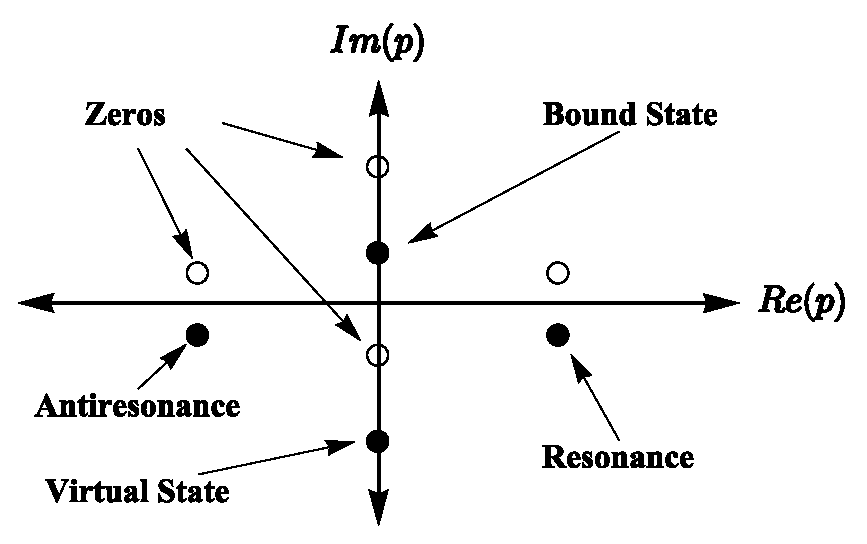
\includegraphics[width=0.75\linewidth]{DiagramPoles.eps}
    \caption{Example of configuration of  poles (filled circles) and zeros (empty circles) of the $S$-matrix eigenvalues in the complex momentum plane for hermitian Hamiltonians.  Poles in the upper half plane ($\operatorname{Im}(p) > 0$) correspond to bound eigenstates of the Hamiltonian, i.e. localized states with negative energy. Poles in the lower half plane correspond to  virtual states ($\operatorname{Re}(p) = 0$), resonances ($\operatorname{Re}(p) > 0$) and antiresonances ($\operatorname{Re}(p)<0$). The singularities with negative imaginary part correspond to states that do not belong to the Hilbert space since they are not normalizable. However, they can produce observable effects in the scattering amplitudes, in particular when they approach the real axis. The pole structure of symmetries IV, V, and VII, see Table I,
is similar, but pole pairs are also possible in the upper half-plane.}
    \label{fig:DiagramPoles}
\end{figure}

%however generally do not conserve norm, and typically have complex eigenvalues and asymmetrical singularities of $S$.
%Surprisingly, as . After the proposal to realize PT-symmetric Hamiltonians
%in optical waveguides with gain and loss \cite{ruschhaupt2005physical}, the experimental realization of PT-symmetric structures has found many applications and triggered renewed interest in NH interactions.

% \comment{[Unknown citation here, What is Wang?]}.%\cite{Nixon2016,Chen2017,Yang2017,Wang}

%The reality of eigenvalues and finite matrices has been investigated in \cite{Bender2010}.
%However, arguments valid for finite matrices are not necessarily applicable
%to scattering systems with a continuum spectrum. In scattering systems it is also of interest to determine the general structure of $S$-matrix singularities in the complex momentum plane, including not only eigenvalues of $H$
%in the upper half-plane but also poles in the lower half plane such as resonances, antiresonances, and anti-bound states.
%Moreover, studies on systems with a continuum, often rely on
%local potentials, but non-local potentials are physically meaningful, they follow from Feschbach's projection,
%and offer richer possibilities.


%In this paper we study the symmetry properties of the $S$-matrix in the complex momentum plane for non-hermitian,
%non-local scattering Hamiltonians in one dimension.
%\blue{Specifically the goal of the paper is to show that a family of Hamiltonian symmetries characterized by antiunitary superoperators
%necessarily imply that the $S$-matrix singularities are either real or appear in conjugate pairs \textbf{(This was already noticed by Mostafazadehfazadeh. A new and more ambitious goal would be proving that if the Hamiltonian is invariant under the action of some antilinear superoperator, not necessarily unitary, the eigenenergies are real or come in complex conjugate pairs)}}. This structure implies the stability of bound and antibound states:   under these conditions a single discrete real singularity cannot bifurcate into a complex conjugate pair when deforming the potential.
%A complex pair can only appear when two real eigenvalues collide.

%\red{paper structure here}

The remainder of the article is organized as follows. In section \ref{sec:SymTheory} we review the scattering properties of eight different Hamiltonian symmetries. These symmetries may be characterized as commutativity or pseudohermiticity with respect to four unitary or antiunitary operators forming a Klein $4$-group, or as invariance with respect to the action of eight linear or antilinear superoperators. In section \ref{sec:SPoles} we discuss the physical consequences of the symmetries in the pole structure of the scattering matrix eigenvalues  and hence in the transmission/reflection amplitudes. Four symmetries are shown to lead to complex poles corresponding to real energies or conjugate (energy) pairs.  In section \ref{sep_pot_sec} we exemplify the general results with separable potentials exhibiting parity-pseudohermiticity and time-reversal symmetry. These are the two non-trivial symmetries of the four (in the sense that the other two, hermiticity and PT-symmetry, are already well discussed). In section \ref{sec:RealEigenConclusions} we discuss and summarize our results.

% \red{In section \ref{sec:ConjugatePairs} we prove that Hamiltonians which are invariant under the action of the antilinear superoperators imply symmetrical $S$-matrix pole pairs.}

\begin{table*}
%\label{table2RealEigen}
\centering
\scalebox{1}{
\begin{tabular}{ccccccccccc}
%\hline
1&2&3&4&5&6&7&8&9&10&11
\\
Code & Symmetry&  $\la x|V|y\ra$ & ${\cal{L}}$(coord)& $\la p|V|p'\ra$ & ${\cal L}$(momentum) &$\la p|S|p'\ra$ & $T^l$ & $T^r$ & $R^l$& $R^r$
\\
\hline
I & $1H=H1$ &   $\la x|V|y\ra$ & ${ 1}$ &$\la p|V|p'\ra$ &${ 1}$& $\la p|S|p'\ra$ & $T^l$ & $T^r$ & $R^l$ & $R^r$
\\
II & $1H=H^\dagger 1$ &  $\la y|V|x\ra^*$ & ${\cal TC}$& $\la p'|V|p\ra^*$ &${\cal T'C'}$&$\la p|\widehat{S}|p'\ra$ & $\widehat{T}^l$& $\widehat{T}^r$ & $\widehat{R}^l$ & $\widehat{R}^r$
\\
III & $\Pi H=H\Pi$ &  $\la -x|V|-y\ra$ &${\cal I}$&  $\la -p|V|-p'\ra$ &${\cal I'}$&$\la -p|S|-p'\ra$ & $T^r$ & $T^l$ & $R^r$ & $R^l$
\\
IV & $\Pi H=H^\dagger \Pi$ &  $\la -y|V|-x\ra^*$ &${\cal CTI}$& $\la -p'|V|-p\ra^*$ &${\cal C'T'I'}$& $\la -p|\widehat{S}|-p'\ra$ & $\widehat{T}^r$ & $\widehat{T}^l$ & $\widehat{R}^r$ & $\widehat{R}^l$
\\
V & $\Theta H=H\Theta$ &  $\la x|V|y\ra^*$&${\cal C}$& $\la -p|V|-p'\ra^*$ &${\cal I'C'}$& $\la -p'|\widehat{S}|-p\ra$ & $\widehat{T}^r$ & $\widehat{T}^l$ & $\widehat{R}^l$& $\widehat{R}^r$
\\
VI & $\Theta H=H^\dagger\Theta$ &  $\la y|V|x\ra$&${\cal T}$& $\la -p'|V|-p\ra$ &${\cal I'T'}$& $\la -p'|S|-p\ra$ & $T^r$& $T^l$ & $R^l$& $R^r$
\\
VII & $\Theta\Pi H=H\Theta \Pi$ &  $\la -x|V|-y\ra^*$ &${\cal IC}$& $\la p|V|p'\ra^*$ &${\cal C'}$& $\la p'|\widehat{S}|p\ra$ &$\widehat{T}^l$& $\widehat{T}^r$ & $\widehat{R}^r$& $\widehat{R}^l$
\\
VIII& $\Theta\Pi H=H^\dagger \Theta \Pi$ &  $\la -y|V|-x\ra$ &${\cal IT}$& $\la p'|V|p\ra$ &${\cal T'}$& $\la p'|S|p\ra$ & $T^l$ & $T^r$ & $R^r$ & $R^l$
%\\
%\hline
\end{tabular}
}
\caption{Symmetries of the potential based on the commutativity or pseudohermiticity of $H$ with the elements of $\mathbf{K}_4$ (column 2). Columns 3, 5, and 7 to 11 are to be read as follows: For each symmetry the object in the column is equal to the one in the top row of the column. The relations among potential matrix elements are given in coordinate and momentum representations in the third and fifth columns. In columns 4 and 6, each symmetry is regarded as the invariance of the potential with respect to the transformations represented by superoperators ${\cal L}$ (see Sec. \ref{super}) in coordinate  or momentum  representation.
The fifth column gives the relations they imply in the matrix elements of $S$ and $\widehat{S}$ matrices. The final four columns set the relations for the scattering amplitudes.
\vspace*{.2cm}
\label{table2RealEigen}}
%\end{tabular}
%}
\end{table*}
% -------------------------------------------------------------------------------------------------

\section{Hamiltonian Symmetries}
\label{sec:SymTheory}
%
\subsection{Basic concepts and terminology}
%
Let us first clarify the terminology. Scattering Hamiltonians are the ones that can be written as the sum of kinetic energy $H_0 = {p^2}/({2m})$ operator and a potential energy operator $V$,
%
\begin{equation}
    H = H_0 + V.
    \label{eq:ScatteringHamiltonian}
\end{equation}
%
$V$ is in general non-local, i.e., it does not have the local form $\la x|V|x'\ra=\delta(x-x')V(x)$.
%Non-local potentials may be as physical as non-hermitian ones, and appear generically in Feshbach formalism as effective interactions \cite{feshbachPQ1,feshbachPQ2}. Non-local potentials also arise in the analysis of molecular orbits when using the Hartree-Fock theory \red{old stuff, difficult to find good refs.}.
Apart from their generic appearance in Feschbach's partitioning technique, see e.g. \cite{Ruschhaupt2004a},
non-local potentials   are quite common in models that discretize the coordinates at specific sites, as in tight-binding models.
These are widely used for describing condensed matter and ultracold atoms in a lattice. For example, the well known Bose-Hubbard model has been generalized to a non-Hermitian Hamiltonian to account for dissipation effects, see e.g. \cite{Hiller2006,Zhong2011}. However, here we limit ourselves to continuous-coordinate scattering models.\footnote{
Also, discrete Hamiltonian matrix models abound in many fields, for example quantum optics, in which rather than couplings
among different ``sites'' there are couplings among states or levels.
Thus a generalized concept of ``non-locality'' may be applied,
as being equivalent to non-zero non-diagonal elements in the chosen basis. The non-Hermitian symmetry groups in these discrete models
can be larger than the set of symmetries based on Eqs. (\ref{gs1}) and (\ref{gs2}) described here, which are constrained by the structure of $H_0$. Discrete model symmetries, interesting as they are, and
with potential applications in condensed matter, optics, or quantum optics,
lie beyond the scope of this work and need a deeper separate study.}
The potential function in position coordinates $V(x,x') = \bra{x}V\ket{x'}$ is assumed to decay fast enough to 0 when a position goes to infinity so that the usual operators of scattering theory are well defined and the Hilbert space is (biorthogonally) decomposed into a continuum
part with real eigenvalues and a discrete part. See Appendix \ref{sec:ScattFormalism} for a review of the formalism and notation we use.

We will now discuss the eight symmetries identified in \cite{Ruschhaupt2017},
which are associated with the two generalized symmetry relations corresponding to commutation with $A$ and $A$-pseudohermiticity \cite{Mostafazadeh2002}, see Eqs. (\ref{gs1},\ref{gs2}).
%
%\begin{eqnarray}
%AH&=&HA,
%\label{gs1}
%\\
%AH&=&H^\dagger A,
%\label{gs2}
%\end{equation}a
%
%where $A$ is a unitary or antiunitary operator in Klein $4$-group $\mathbf{K}_4 = \left\{1,\Pi,\Theta,\Theta\Pi\right\}$ formed by the identity ($1$), parity ($\Pi$), time-reversal ($\Theta$) and their product ($\Theta\Pi$), also known as the PT operator.
We use Roman numeral to label these symmetries as shown in Table I: I ($1H=H1$, the trivial identity)
; II ($1H=H^\dagger 1$, hermiticity or ``1-pseudohermiticity''); III ($\Pi H=H\Pi$, parity); IV ($\Pi H=H^\dagger \Pi$, $\Pi$-pseudohermiticity);  V ($\Theta H=H\Theta$, time-reversal invariance);  VI ($\Theta H=H^\dagger \Theta$, $\Theta$-pseudohermiticity);
VII ($\Pi\Theta H=H\Pi\Theta$, PT-symmetry); VIII ($\Pi\Theta H=H\Pi\Theta$, $\Pi\Theta$-pseudohermiticity).
Note that a local potential would automatically fulfill symmetry VI but this symmetry does not necessarily imply locality.
For local potentials four of the eight symmetries coincide with the other four \cite{Ruschhaupt2017}. Here we consider general nonlocal potentials where all the eight symmetries are distinct.


The generalization of the symmetry concept to the pair \eqref{gs1} and \eqref{gs2} is in fact quite natural if we take into account that a NH-$H$
has generically different left and right eigenvectors. Given a right eigenstate $\ket{\psi}$ of $H$ with eigenvalue $E$, Eq. (\ref{gs1}) implies that  $A|\psi\ra$ is also a right eigenvector with eigenvalue $E$ or $E^*$, whereas Eq. (\ref{gs2}) implies that $\la \psi|A$ is a left eigenvector of $H$ with eigenvalues $E^*$ or $E$,  for $A$ unitary or antiunitary respectively. \footnote{$A$ is an antiunitary operator if it is an antilinear operator that maps a Hilbert space onto itself satisfying $\expval{A \psi,A\phi}= \expval{\phi,\psi}$ for $\psi$ and $\phi$ in that Hilbert space. It  satisfies $AA^{\dagger}=A^\dagger A=1$, where the adjoint is to be understood as for antilinear operators, namely  $\expval{\phi,A^\dagger\psi} = \expval{\psi,A \phi}$ \cite{Muga2004}.}

The symmetries which imply the presence of real or complex-conjugate pairs of energy eigenvalues for bound eigenstates
are II, IV,V and VII.
The emergence of these complex-conjugate pairs has been previously discussed in \cite{Mostafazadeh2002,Bender2010} for a general class of diagonalizable Hamiltonians that posses a discrete spectrum. They can be heuristically understood for the symmetries we consider as follows: Symmetry V implies that the Hamiltonian must be real in coordinate space, which would lead to a real characteristic polynomial with real or complex-conjugate roots. Symmetry VII is PT symmetry which is well discussed in the literature as having real or complex-conjugate pairs of eigenvalues \cite{Bender1998}. Note also that the matrix elements of PT-symmetric Hamiltonians are real in the momentum representation. More generally, in \cite{Mostafazadeh2002b}, it was shown, for diagonalizable Hamiltonians having a discrete spectrum, that $A$-pseudohermiticity for a Hermitian invertible linear operator $A$ is equivalent to the presence of an ordinary symmetry of the form $BH = HB$ for some antilinear operator $B$ with $B^2 = 1$. Because $B$ is an antilinear operator, the eigenvectors $\ket{E_n}$  of $H$ with eigenvalues $E_n$ satisfy
%
\begin{eqnarray}
H B \ket{E_n}&=&B H \ket{E_n} \nonumber \\
				   &=&E_{n}^{*} B \ket{E_n}.
\end{eqnarray}
%
Therefore complex eigenvalues $E_n$ come in complex-conjugate pairs. In particular, when $\ket{E_n}$  is an eigenvector of $B$, i.e., $B\ket{E_n} = e^{ib_n} \ket{E_n}$ for some real number $b_n$, we have $E_n \in \mathbb{R}$.
The proof of the equivalence of $A$-pseudohermiticity for linear $A$ and the presence of ordinary antilinear symmetries given in \cite{Mostafazadeh2002b} relies on the observation that every diagonalizable Hamiltonian with a discrete spectrum is $\tau$-pseudohermitian for some invertible Hermitian antilinear operator $\tau$, i.e.,
$\tau H = H^\dagger\tau$. This relation together with Eq. (\ref{gs2}) implies $BH = HB$,
if we set $B = A^{-1}\tau$. (If $AH=H^\dagger A$ and $A$ is a Hermitian antilinear operator, a linear $B = A^{-1}\tau$ can also be constructed so that $BH=HB$, but the $E_n$ do not form conjugate pairs.)
In Appendix \ref{app5} we extend this construction to scattering potentials.

In summary, the symmetries with conjugate pairs II, IV, V, and VII can be all expressed as the commutation of $H$ with a certain antilinear operator, as seen directly in the symmetries V and VII, in which $H$ commutes with an antilinear $A$,  and by constructing an antilinear $B$ in the symmetries II and IV.
A novel aspect uncovered in this paper is that whenever one of  the above-mentioned four symmetries holds not only the complex eigenvalues representing the bound states come in conjugate-complex pairs, but all the complex poles of the $S$-matrix have this property.


%These conjugate pairs  have been previously discussed
%e.g. in \cite{Mostafazadeh2002,Bender2010} for discrete Hamiltonians and can be heuristically understood for these symmetries  as follows:  Symmetry II is simply Hermiticity. Symmetry V implies that the Hamiltonian must be real in coordinate space which would lead to a real characteristic polynomial (which must have complex-conjugate roots). Symmetry VII is PT symmetry which is well discussed in the literature as having also complex-conjugate pairs of eigenvalues \cite{Bender1998}, note that the Hamiltonian matrix in this case is real in momentum representation.
%More generally, in \cite{Mostafazadeh2002b}, it was shown for discrete Hamiltonians that symmetries of the form \eqref{gs2}, with $A$ linear imply an ``ordinary'' symmetry of the form $\left[A^{-1}\tau,H\right]=0$, with $\tau$
%antilinear, and a complex part of the spectrum in conjugate pairs. The generalized construction of the antilinear $\tau$ for our scattering  potentials is discussed in Appendix \ref{app5}.
%In other words these particular four symmetries can be written as $GH=HG$ for some  antilinear $G$, so
%
%\begin{eqnarray}
%H G \ket{E_n}&=&G H \ket{E_n} \nonumber \\
%				   &=&E_{n}^{*} G \ket{E_n}.
%\end{eqnarray}
%
%Hence all the eigenvalues in the complex part of the discrete spectrum come in  complex-conjugate pairs in these cases. In particular when $G \ket{E_n}=\ket{E_n}$ we get that $E_n \in \mathbb{R}$.
%The novel aspect uncovered in this paper is that not only  the complex eigenvalues of bound states
%come in conjugate complex pairs, in fact all poles of the $S$-matrix eigenvalues correspond to real energies or to
%conjugate energy pairs for the four mentioned symmetries.
%
%In \cite{Ruschhaupt2017} it was shown that these eight symmetries determine selection rules that forbid or allow asymmetries in the
%moduli of the transmission $T^{l,r}(p>0)$ and reflection $R^{l,r}(p>0)$ scattering amplitudes for left and right incidence
%with energy $E_p=p^2/(2m)$.  In this paper we shall focus instead on their implications in the structure of poles and zeroes of the
%$S$-matrix eigenvalues.
%
%
%
\subsection{Superoperator formalism \label{super}}
%
%
%
The eight symmetries listed in Table I may also be regarded as the invariance
of the Hamiltonian matrix with respect to
transformations represented by superoperators ${\cal L}$ \cite{Simon2018} defined by
%
\begin{eqnarray}
\mathcal{L}(H)=
	\begin{cases}
      A^\dagger H A &  \text{I, III,V,VII} \\
      A^\dagger H^\dagger A &\text{II, IV, VI, VIII}
   \end{cases}.
\end{eqnarray}
%
%\red{Write how the symmetries look like using the superoperator formalism in position and mommentum basis.}
%
%
%We adhere to the simple definition of symmetry as stated by Feynman, which he attributed to Weyl:
%``a thing is symmetrical if one can subject it to a certain operation and it appears exactly the same after the operation'' \red{citation}.
This definition of the superoperator action is independent of the representation we use, but its realization
in coordinates or momenta in terms of the operations of complex conjugation, transposition, and inversion is different.
For example, in coordinate representation, these superoperators take the following forms (see column 3 in Table I),
%
\begin{eqnarray}
1 H&=&\int\!\!\int |x\ra \la x|H|y\ra\la y| dx dy,
\nonumber\\
{\cal T} (H) &=&\int\!\!\int |x\ra \la y|H|x\ra\la y| dx dy,
\nonumber\\
{\cal C} (H)&=&\int\!\!\int |x\ra \la x|H|y\ra^*\la y| dx dy,
\nonumber\\
{\cal I} (H)&=&\int\!\!\int |x\ra \la -x|H|-y\ra\la y| dx dy.
%\nonumber\\
%{\cal CT} H &=&\int\!\!\int |x\ra \la y|H|x\ra^*\la y| dx dy,
%\nonumber\\
%{\cal CI} H&=&\int\!\!\int |x\ra \la -x|H|-y\ra^*\la y| dx dy,
%\nonumber\\
%{\cal TI} H&=&\int\!\!\int |x\ra \la -y|H|-x\ra\la y| dx dy,
%\nonumber\\
%{\cal CTI} H&=&\int\!\!\int |x\ra \la -y|H|-x\ra^*\la y| dx dy,
\label{defs}
\end{eqnarray}
%
% inner product for linear operators F and G, hhF|Gii = trF�G, we can show that all the above superoperators L are either unitary (for L = 1, T , I, T T ) or antiunitary ( for {\cal L} = C, CT , CI, CT I). Recall the following definition of unitarity and antiunitarity.
Adopting the following inner product for linear operators $F$ and $G$, $\langle\langle F|G\rangle\rangle={\rm{tr}} F^\dagger G$,
we can show that all superoperators ${\cal L}$ are either unitary (for ${\cal L}=1,{\cal T},{\cal I},{\cal TI}$), or antiunitary (for ${\cal L}={\cal C}, {\cal CT},{\cal CI},{\cal CTI}$), as defined by
%
\begin{eqnarray}
\langle\langle {\cal L}F| {\cal L}G\rangle\rangle&=& \langle\langle F| G\rangle\rangle\;\;\;  ({\cal L}\; {\rm unitary}),
\\
\langle\langle {\cal L}F| {\cal L} G\rangle\rangle&=& \langle\langle  F| G\rangle\rangle^*\;\;\;  ({\cal L}\; {\rm antiunitary}).
\end{eqnarray}
%
%where antiunitary  superoperators satisfy
%%
%\beq
%{\cal L} (aA_1+bA_2)=a^*{\cal L}A_1+ b^*{\cal L}A_2.
%\eeq
%
They all satisfy ${\cal L}{\cal L}^\dagger={\cal L}^\dagger {\cal L}=1$
where the adjoints are defined differently for linear or antilinear superoperators,
\begin{eqnarray}
\langle\langle F| {\cal L}^\dagger G\rangle\rangle&=& \langle\langle {\cal L} F| G\rangle\rangle\;\;\;  ({\cal L}\; {\rm unitary}),
\\
\langle\langle F| {\cal L}^\dagger G\rangle\rangle&=& \langle\langle {\cal L} F| G\rangle\rangle^*\;  ({\cal L}\; {\rm antiunitary}).
\end{eqnarray}
%
Moreover the eight superoperators  satisfy ${\cal L}^\dagger={\cal L}$.

The set $\{1, \cal{I,T,C,CT,TI,IC,CTI}\}$ forms the elementary abelian group $E8$ \cite{Rose2009}.
%and cite. Ref: Rose, H. E. A course on finite groups. Springer-Verlag: London, UK, 2009, ISBN 978-1-84882-888-9.}.
This is a homocyclic group, namely, the direct product of isomorphic
cyclic groups of order 2 with generators $\cal{C,T,I}$. We may, similarly to Eq. (\ref{defs}), define primmed superoperators in momentum representation, e.g. ${\cal T'} H =\int\!\!\int |p\ra \la p'|H|p\ra\la p'| dp dp'$. They also form the E8 group
$\{1, \cal{I',T',C',C'T',T'I',I'C',C'T'I'}\}$. Only for the subgroup $\{1, \cal{I,CT,CTI}\}$ the superoperators have the same representation-independent form in terms of complex conjugation, transposition and inversion.

A direct application of the superoperator framework is the generalization of Wigner's
formulation of symmetries \cite{Wigner1959}. He associated symmetry transformations to unitary or antiunitary operators preserving the (Hilbert space) inner product, namely the ``transition probabilities'' $|\expval{A\psi,A\phi}|^2=|\expval{\psi,\phi}|^2$.
For general states described by density operators $\rho_1,\rho_2$, transition probabilities are computed as $\la\la \rho_1|\rho_2\ra\ra$
and the transformations described by the unitary or antiunitary superoperators preserve the
transition probability. Hamiltonian symmetries are, within the conventional Wigner scheme, the  symmetry transformations that leave the Hamiltonian invariant ($A^\dagger H A=H$, so that $A$ and $H$ commute). Here the Hamiltonian symmetry is more broadly defined  as
the invariance ${\cal L}H=H$, which includes transformations  beyond the conventional scheme.


%
%
%

%A further alternative view of the eight symmetries generalizes results found for discrete Hamiltonians that show that
%symmetries of the form (\ref{gs2}) may in fact be also formulated as commutation relations between $H$ and certain operators, linear
%for antilinear $A$, and antilinear for linear $A$. The generalization for scattering Hamiltonians and the explicit construction
%of the operator that commutes with $H$ is worked out in the Appendices.
%
\section{S-matrix pole structure}
\label{sec:SPoles}
%
%One of the most studied aspects of the collisions with non-hermitian potentials is the meaning
%of poles of $S_j(p)$ in the complex plane $p$ and their motions. In the unitary case
%the poles of the amplitudes $S_j(p)$ are classiffied according to their position in the plane: the poles
%on the positive imaginary axis correspond to bound states, those in the fourth quadrant to resonances,
%and in the third quadrant to antiresonances. The non-unitary case presents new possibilities:
%poles in the first  quadrant, corresponding to states whose norm grows exponentially with time, and
%poles in the second quadrant, corresponding to states whose norm decreases with time [31]. The poles
%in the upper half-plane are on the first  Riemann sheet of the energy so the corresponding energy
%belongs to the point spectrum of $H$. In the hermitian case ($S =\widehat{S}$) the poles in the lower momentum
%half-plane come in symmetrical pairs with respect to the imaginary axis, with zeroes in the upper
%half-plane at conjugate positions but this symmetrical pattern is broken
%in general for non-hermitian Hamiltonians. Exceptions to this will be presented in Section .... .
%
%
To derive the results in \cite{Ruschhaupt2017} an extensive use of the scattering matrix ($S$-matrix) formalism was made. The full $S$-matrix
provides outgoing waves when acting on incoming waves. It is typically decomposed into on-the-energy-shell matrices.
%is simply the operator that acting on an incoming wave function gives the resulting wave function after the scattering has taken place. The relations in \eqref{gs1} and \eqref{gs2} imply certain intertwining relations of the $S-$matrix with the elements of the Klein's group that lead to the selection rules in  \cite{Ruschhaupt2017}.}
In 1D scattering, the on-the-energy-shell $\sf{S}(p)$ matrix for $H$ is defined on the real positive momentum axis in terms of transmission and reflection amplitudes for right
and left incidence \cite{Muga2004},
%
\begin{equation}
\sf{S}=\left(\begin{array}{cc}
T^l(p)&R^r(p)
\\
R^l(p)&T^r(p)
\end{array}\right).
\end{equation}
%
There is a companion matrix $\widehat{\sf{S}}$ with hatted amplitudes corresponding to scattering by $H^{\dagger}$. See Appendix \ref{sec:ScattFormalism} and \cite{Muga2004} for details. The $\sf{S}$ matrix contains the scattering amplitudes for incoming wave packets with well defined momentum being scattered into states with the same kinetic energy and reflected and transmitted components.
%
For negative $p$ the matrix elements give the amplitudes of scattering states with a pure outgoing plane wave towards the right or the left.
Moreover we assume, as it is customary,
that the amplitudes may be continued analytically beyond the real axis.
The existence of a continuation on a complex plane domain depends on decay properties of the potentials and may
be checked for each potential.
The analytical continuation is indeed possible for the model potentials of the following section.



The eigenvalues of $\sf{S}$ can be calculated from the transmission and reflection amplitudes as
%
\begin{equation}
S_j=\frac{(T^l+T^r)+(-1)^j[(T^l-T^r)^2+4R^lR^r]^{1/2}}{2}
\label{Sform}
\end{equation}
%
for $j=1,2$, and of course there is a similar expression for $\widehat{S}_j$ with hatted amplitudes.
In general they satisfy the relations \cite{Muga2004},
%
\begin{equation}\label{pam1}
S_j(p)=\widehat{S}_j^*(-p^*)\,,
\end{equation}
%
and
%
\begin{equation}\label{pam2}
\widehat{S}_j^*(p^*)S_j(p)=1\,.
\end{equation}
%
Combining Eqs. (\ref{pam1}) and (\ref{pam2}) gives
%
\begin{equation}\label{pam3}
S_j(p)=S^{-1}_j(-p)\,.
\end{equation}
%
Equation \eqref{pam3} is remarkable since it reveals the presence of a pole (zero) at $-p$ if there is a zero (pole) at $p$.
%
%Of
%Generalizing the concept of symmetry for NH-Hamiltonians, eight symmetries are identified, see Table I,
%among which four imply
%a structure for poles and zeros of the S matrix compatible with the existence of real, discrete eigenvalues, more specifically, the discrete eigenvalues
%appear necessarily in conjugate pairs. Two of these
%four symmetries are well known, namely, hermiticity and PT-symmetry, whereas the other two types are denominated here as parity pseudohermiticity (symmetry type IV)
%and time-reversal invariance (symmetry type V).
If the following relations are fulfilled,
%
\begin{eqnarray}
T^{r,l}(p)&=&\widehat{T}^{r,l}(p)\; {\rm or}\; T^{r,l}(p)=\widehat{T}^{l,r}(p),
\label{ts}
\\
R^{r,l}(p)&=&\widehat{R}^{r,l}(p)\; {\rm or}\; R^{r,l}(p)=\widehat{R}^{l,r}(p),
\label{rs}
\end{eqnarray}
%
then
%
\begin{equation}
S_j(p)=\widehat{S}_j(p),
\end{equation}
%
which together with Eq. \eqref{pam1} gives
%
\begin{equation}
S_j(p)=S_j^*(-p^*).
\label{eq:PoleSymmetry}
\end{equation}
%}
In plain language, Eq. \eqref{eq:PoleSymmetry} tells that if Eqs. (\ref{ts}) and (\ref{rs}) are satisfied,  the poles and zeros of $S_j$ must be symmetrically distributed with respect to the imaginary axis of momentum complex plane. Combined with Eq. (\ref{pam3})
this also means that each pole has a symmetrical zero with respect to the real axis. This symmetrical distribution of poles and zeros is the same as in the Hermitian case (see Fig. \ref{fig:DiagramPoles}),
%end red
the only difference being the possibility
of finding pairs of symmetrical poles in the upper complex plane when $H\neq H^\dagger$. They represent normalizable ``bound states
with complex energies''. When they  are not present, the discrete spectrum becomes purely real.

According to Table I,  Eqs. (\ref{ts}) and (\ref{rs}) are fulfilled
for symmetries  II (hermiticity), VII (PT-symmetry), IV (parity pseudohermiticity),
and V (time-reversal invariance). Thus, Hamiltonians having these symmetries have their $S-$matrix poles symmetrically distributed around the imaginary axis. For local potentials the last two symmetries coalesce with the first two well-known
cases \cite{Ruschhaupt2017}, namely,
IV becomes equivalent to PT-symmetry, and V becomes equivalent to hermiticity. For non-local potentials, though, these symmetries
correspond to genuinely distinct properties. In the following section we shall demonstrate this fact with potentials that are
either purely parity-pseudohermitian (and not PT-symmetrical), or time-reversal invariant but not Hermitian.

%
%we get
%%
%\begin{eqnarray}\label{prt1}
%(R^{l,r}(p))^* &=& \widehat{R}^{l,r}(-p^*)\,, \nonumber\\
%(T^{l,r}(p))^* &=& \widehat{T}^{r,l}(-p^*)\,,
%\end{equation}a
%%
%%
%The generalization  of the unitarity relation (\ref{uni})
%in the different representations of the scattering operator
%(\ref{mco1},\ref{mco2}) provides another series of relations
%between the amplitudes: for the plane wave
%representation,\footnote{
%If $f(z)$ is
%analytic in a region ${\cal D}$, $f^*(z^*)$ will be
%analytic in ${\cal D}^*$.}
%%
%\begin{eqnarray}\label{prt2}
%\widehat{T}^{l*}(p^*)T^l(p)+\widehat{R}^{l*}(p^*)R^l(p) &=& 1\,, \nonumber\\
%\widehat{T}^{l*}(p^*)R^r(p)+\widehat{R}^{l*}(p^*)T^r(p) &=& 0\,, \nonumber\\
%\widehat{R}^{r*}(p^*)T^l(p)+\widehat{T}^{r*}(p^*)R^l(p) &=& 0\,, \nonumber\\
%\widehat{R}^{r*}(p^*)R^r(p)+\widehat{T}^{r*}(p^*)T^r(p) &=& 1\,,
%\end{equation}a
%%
%and for the diagonal representation
%
%
%
%
%
%
\section{Separable Potentials}
\label{sep_pot_sec}
%
%
In order to illustrate and test the theoretical concepts that we have discussed, in particular the
symmetrical configuration of poles with respect to the imaginary axis in the complex momentum plane for certain Hamiltonian symmetries, we will use some solvable toy models consisting on rank-one separable potentials.
Separable potentials are quite useful models as a solvable approximation to realistic ones, in particular in nuclear, atomic and molecular physics \cite{Popov2019}.
Often they lead to explicit expressions
for wave functions or scattering amplitudes, so they are used to test concepts and new methods.
They are also instrumental in learning about different dynamical phenomena (for example transient effects, short-time and long-time behavior, or anomalous decay laws)  and their relation to complex-plane singularities
\cite{Muga1990,Muga1996,Muga1996b,Muga1998a}. Their simplest version takes the form
$|\chi\ra V_0\la\chi|$ for some  $\chi$.   In particular, with a complex $V_0$,
they have been used to examine anomalous (negative) time delays caused by  crossing of zeroes of the $S$-matrix eigenvalues or $S$-matrix elements across the momentum real axis \cite{Muga1998b}.

In this work we consider the simple structure
$V=V_0 \ketbra{\phi}{\chi}$, with $V_0$ (potential strength) real, and conveniently chosen functions $\phi$, $\chi$.
The aim of this section is to demonstrate the formal results of the previous section without attempting to simulate any specific systems, but we note that separable, NH potentials are instrumental to model nuclear reactions, in particular  by increasing the rank (number of separable terms) \cite{Hlophe2017}.
Separable NH potentials also provide solvable approximations to nonlocal NH potentials that arise naturally in quantum optics to describe the interaction of a ground state atom with a laser beam \cite{Ruschhaupt2004a}.
%,
%but these connections and the physical implementation are left for a separate publication.
%endred
%
%In later publications we  in the very  get delving into any specific , in particular the
%symmetrical configuration of poles with respect to the imaginary axis in the complex momentum plane for certain Hamiltonian symmetries.
%In passing we shall also note some interesting phenomena that may be studied in more detail elsewhere, such as pole collisions, crossings of
%the real axis, or diodic (Maxwell demon) behavior with asymmetrical transmission for right/left incidence.
%
%\cite{Muga1990,Muga1996,Muga1996b,Muga1998a}.
In passing we shall also note some interesting phenomena that may be studied in more detail elsewhere, such as pole collisions, crossings of
the real axis, or diodic (Maxwell demon) behavior with asymmetrical transmission for right/left incidence.
%Rank-one separable potentials are objects like
%
%\begin{equation}
%  V =  V_{0} \ket{\phi}\bra{\psi},
%\end{equation}
%
%where $V_0$ is a complex valued coefficient and $\ket{\phi}$, $\ket{\psi}$ some normalized states. Althought we are using separable potentials as toy models, it is relevant to mention that they are used extensively to approximate many body interactions in nuclear and condensed matter physics \cite{Maghari_2008,Maghari_2005,Muga1998b,Elster_2016,PhysRevC.88.064608,PhysRevC.93.034601,PhysRevC.95.054617,PhysRevC.96.064003}. In the nuclear scattering context, the state vectors $\ket{\psi}$ and $\ket{\phi}$ correspond to single-channel incoming and outgoing scattering wave functions respectively \cite{PhysRevC.95.054617}. The main reason why we have chosen separable potentials is that, because of their simplicity, it is possible to find analytical expressions for the scattering amplitudes, see Appendix \ref{app1}. For this paper we have taken $V_0$ to be real so that it could be interpreted as the potential strength.

From the stationary Schr\"{o}dinger equation $H \ket{\psi} = E \ket{\psi}$, the eigenvalues of separable potentials may be found by solving
%
\begin{eqnarray}
Q_{0}(E)V_{0} = 1,
\label{roots}
\end{eqnarray}
%
where $Q_{0}(E)=\bra{\chi}(E-H_0)^{-1}\ket{\phi}$ and $H_{0}=p^{2}/(2m)$. Moreover, for a separable potential, the transition operator $T_{op}$ can be written (see Appendix \ref{app1}) as
%
\begin{equation}
T_{op}=\frac{V_{0}}{1-V_{0} Q_{0}(E)} \ketbra{\phi}{\chi}.
\end{equation}
%
Since all scattering amplitudes in $S$ are simply related to matrix elements of $T_{op}$ in momentum representation, see
Eq. (\ref{art}), solutions to Eq. (\ref{roots}) provide their core singularities (independent of the representation \cite{Muga1996}).
%In the upper momentum plane they correspond to the discrete spectrum of $H$. In the lower half-plane they are
%resonances (fourth  quadrant), antiresonances (third quadrant), or virtual states (on the imaginary axis).
Once $Q_{0}(E)$  is calculated, the transmission and reflection amplitudes can be found from \eqref{art}
using the momentum representation of $\ket{\phi}$ and $\ket{\chi}$.

In the following subsections we will build a Hamiltonian with symmetry V (time reversal) and another one with symmetry IV
(parity pseudohermicity) and illustrate the symmetries of the $S$ matrix poles in momentum complex plane.



% From the stationary Schr\"{o}dinger equation $H \ket{\psi} = E \ket{\psi}$, the eigenvalues may be found by solving
% %
% \begin{eqnarray}
% Q_{0}(E)V_{0} = 1,
% \label{roots}
% \end{eqnarray}
% %
% where $Q_{0}(E)=\bra{\chi}(E-H_0)^{-1}\ket{\phi}$ and $H_{0}=p^{2}/(2m)$.
%
% Moreover, for a separable potential $V_0 \ketbra{\phi}{\chi}$, the transition operator $T_{op}$ can be written (see Appendix \ref{app1}) as
% %
% \begin{equation}
% T_{op}=\frac{V_{0}}{1-V_{0} Q_{0}(E)} \ketbra{\phi}{\chi}.
% \end{equation}
% %
% Since all scattering amplitudes in $S$ are simply related to matrix elements of $T_{op}$ in momentum representation, see
% Eq. (\ref{art}), solutions to Eq. (\ref{roots}) provide their core singularities (independent of the representation \cite{Muga1996}).
% %In the upper momentum plane they correspond to the discrete spectrum of $H$. In the lower half-plane they are
% %resonances (fourth  quadrant), antiresonances (third quadrant), or virtual states (on the imaginary axis).
%
% Once $Q_{0}(E)$  is calculated, the transmission and reflection amplitudes can be found from \eqref{art}
% using the momentum representation of $\ket{\phi}$ and $\ket{\chi}$.
%
%
%
\subsection{Time-reversal symmetric potential}
%
%
\begin{figure}[h]
    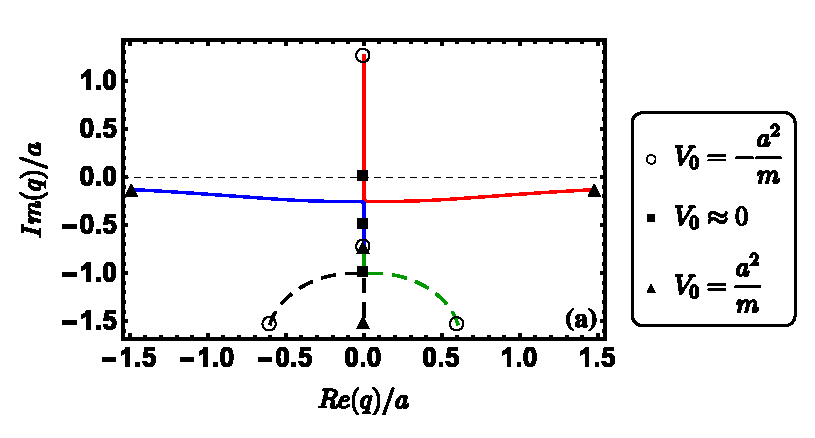
\includegraphics[width=1.0\linewidth]{VSymEigenvalsVaryingV0_Momentum.eps}
    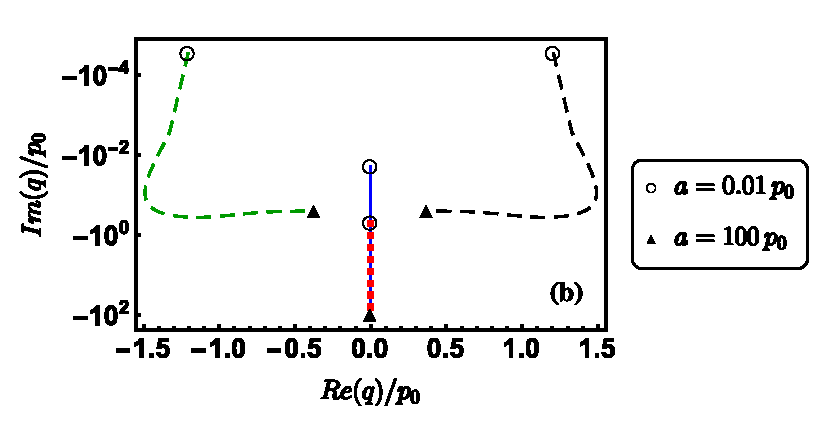
\includegraphics[width=1.0\linewidth]{VSymEigenvalsVaryingA_Momentum_Log.eps}
    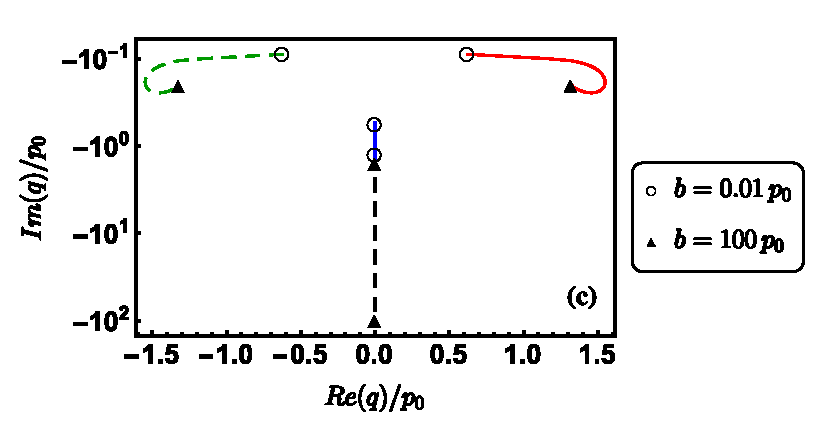
\includegraphics[width=1.0\linewidth]{VSymEigenvalsVaryingB_Momentum_Log.eps}
    \caption{(Color online) Poles and pole trajectories of time-reversal symmetric potential \eqref{TRpot} for (a) varying $V_0$ with $a=2 b$; (b) varying $a$ with $b=0.5\, p_0$, $V_0>0$; and (c) varying $b$ with $a=p_0$,
    $V_0>0$. At pole collisions we connect each of the incoming trajectories with a different emerging trajectory but the choice of outgoing branch  is arbitrary since the two colliding poles lose their identity.}
    \label{fig:VSymEigenvals}
\end{figure}

We start with an example of a separable potential which only satisfies symmetry V (apart from the trivial symmetry I). The normalised vector $\ket{\chi}$, is given in position and momentum representation as
%
\begin{eqnarray}
\braket{x}{\chi}&=&\sqrt{\frac{a}{\hbar}} e^{-a \left| x \right|/\hbar},
\nonumber \\
\braket{p}{\chi}&=& \sqrt{\frac{2 a^3}{\pi}} \frac{1}{p^2+a^2}.
\end{eqnarray}
%
We choose $\ket{\phi}$ similarly as
%
\begin{eqnarray}
\braket{x}{\phi}=&\sqrt{\frac{2ab}{\hbar (a+b)}} \begin{cases}
 e^{-b x/\hbar} &x>0,\\ e^{a x/\hbar}  &x<0,
   \end{cases}\nonumber \\
\braket{p}{\phi}=& \sqrt{\frac{ab}{\pi (a+b)}}\frac{a+b}{(p+i a)(p-i b)}.
\end{eqnarray}
%
The real and positive parameters $\hbar/ a$ and $\hbar/ b$ determine the width of the potential functions in coordinate representation.
$b$ is chosen different from $a$ to introduce a right/left  asymmetry in $\braket{x}{\phi}$.
In coordinate representation the potential is given as
%
\begin{eqnarray}
\la x|V|y\ra = V_{0} \sqrt{\frac{2 b a^2}{\hbar^2 (a+b)}} \begin{cases}
 e^{-(a \left| y \right|+b x)/\hbar} \, &x>0,\\ e^{a (x-\left| y \right|)/\hbar} \,  &x<0.
   \end{cases} \label{TRpot}
\end{eqnarray}
%
%which can be seen in Fig. \ref{fig:VSymPotentialPlot}.
Clearly the potential is always even in $y$ and in the limiting case where $a=b$, it is also even in $x$. For $a=b$, the potential will satisfy parity symmetry (III) and also PT symmetry (VII), without asymmetric transmission or reflection.
% so we ignore it hereafter.

We define first a complex momentum $q=\sqrt{2 m E}$ (for complex $E$) with positive imaginary part.
To calculate $Q_{0}(q)$ explicitly we use a closure relation in momentum representation, and
complex contour integration around the poles at $ia$, $q$ and $ib$.
The result is then analytically continued to the whole $q$-plane,
%
\begin{eqnarray}
&&Q_{0}(q)/m=
\nonumber\\
&&-\frac{i \sqrt{2b} \left[2 a (a+b)^2-q^2 (3 a+b)-i q (2 a+b) (3 a+b)\right]}{q (a+b)^{3/2} (a-i q)^2 (b-i q)},
\nonumber\\
\label{eq:ResolvantVSymm}
\end{eqnarray}
%
with which we may calculate the transmission and reflection amplitudes.
The four roots of Eq. (\ref{roots}) are the core poles.

Using $m$, $V_0$ and $\hbar$ we define the length and momentum scales $L_0 = \hbar/\sqrt{mV_0}$ and $p_0 = \sqrt{mV_0}$. In Fig. \ref{fig:VSymEigenvals}(a), we can see the trajectory of the $S$-matrix core poles (zeros
of $1-V_0Q_0(q))$ for varying $V_0$. Notice a bound state for $V_0<0$ and collisions of the eigenvalue pairs around $V_0 = 0$. In Figs. \ref{fig:VSymEigenvals}(b) and \ref{fig:VSymEigenvals}(c), where $V_0$ is positive and $a$ or $b$ are varied,
there are two virtual states and one resonance/anti-resonance pair. In all cases the symmetry of the poles about the imaginary axis
% for fig. \ref{fig:VSymEigenvals},
which corresponds to real energies or complex-conjugate pairs of energies, is evident. For larger values of the $a$ or $b$ parameters
(not shown)
the pair collides so that all poles end up as virtual states.

Figure \ref{fig:VSymScattAmplitudes} depicts the associated transmission and reflection coefficients (square moduli of the amplitudes) as functions of the momentum $p$. $|R^l(p)|=|R^r(p)|$ for all $p$ due to symmetry V \cite{Ruschhaupt2017}.
The coefficients can be greater than one in contrast to the Hermitian case.

%%%%%%%%%%%%%%%%%%%%%%%%%%%%%%%%%%%%%%%%%%
%Figure
%%%%%%%%%%%%%%%%%%%%%%%%%%%%%%%%%%%%%%%%%%
\begin{figure}
    \begin{center}
    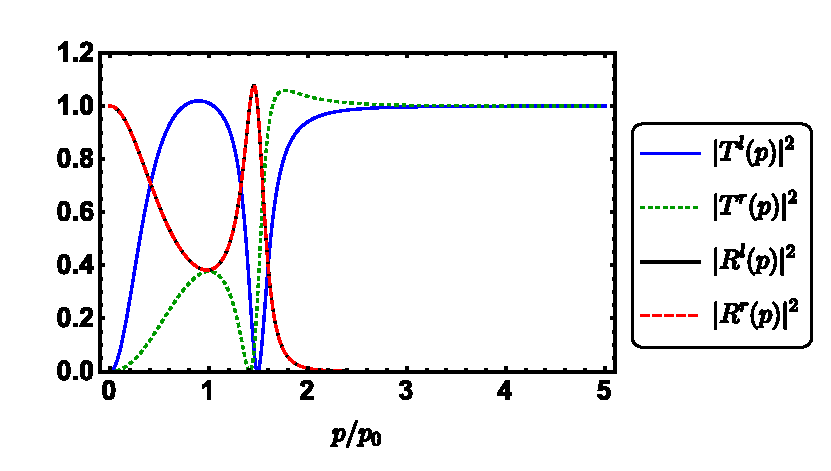
\includegraphics[width=1\linewidth]{VSymScattAmplitudes.eps}
    \end{center}
    \caption{(Color online) Transmission and reflection coefficients of the time-reversal symmetric potential \eqref{TRpot} with $a=p_0$, $b= 0.5\, p_0$ and $V_0>0$.}
    \label{fig:VSymScattAmplitudes}
\end{figure}
%%%%%%%%%%%%%%%%%%%%%%%%%%%%%%%%%%%%%%%%%%

% From Eq. \eqref{pam3}, at $p=0$ the $S$-matrix eigenvalues must be either $\pm 1$. Since $S_2=1$ for all values of $p$ (See Appendix \ref{app2}), $S_1=-1$ at $p=0$. Also, since there is full transmission for very high kinetic energies, $S_j \rightarrow 1$ as $p \rightarrow \infty$. The crossover into the regime where the kinetic energy dominates occurs for  $E_p \gg V_0$, i.e. when $p/p_0 \gg \sqrt{2}$.
% %
%
\subsection{Parity pseudohermitian potential}
%
%
As a second example we will consider  a separable potential which only fulfils symmetry IV. The normalised vector $\ket{\chi}$ in position and momentum representation is
%
\begin{eqnarray}
\braket{x}{\chi}=& \sqrt{\frac{a}{\hbar}} \begin{cases}
e^{-(a+ib)x/\hbar}  &x>0,\\ e^{a x/\hbar} &x<0,
   \end{cases} \nonumber \\
\braket{p}{\chi}=&  \sqrt{\frac{a}{2\pi}} \frac{2 a+ i b}{(p+ia)(p+b-i a)},
\end{eqnarray}
%
where $a>0$ and $b$ is real.
We choose $\ket{\phi}$ as
%
\begin{eqnarray}
\braket{x}{\phi}=& \sqrt{\frac{a}{\hbar}} \begin{cases}
e^{-a x/\hbar} &x>0,\\ e^{(a+i b)x/\hbar} &x<0,
   \end{cases} \nonumber \\
\braket{p}{\phi}=& \sqrt{\frac{a}{2\pi}} \frac{2 a+i b}{(p-ia)(p-b+i a)},
\end{eqnarray}
%
where $\hbar/a$ gives as before the width in coordinate representation. The potential functions in coordinate representation become asymmetrical
because of the  imaginary terms  $ib$ in  the exponent added only on  one side. This term leads to oscillations in real and imaginary parts. In momentum representation $b$ appears as a real shift in the position of one of the poles.
%
In coordinate representation the potential is
%
\begin{eqnarray}
\hspace*{-0.6cm}\la x|V|y\ra=  \frac{aV_{0}}{\hbar} \begin{cases}
 e^{-\left[a (x+y) - i b y\right]/\hbar} \, ,&x>0,\,y>0\\
 e^{a(y-x)/\hbar} \,  ,&x>0, \,y<0\\
 e^{\left[a(x-y)+i b(x+y)\right]/\hbar} \,  ,&x<0,\,y>0\\
 e^{\left[a(x+y)+i b x\right]/\hbar} \,  ,&x<0,\,y<0
   \end{cases}.
   \label{Ppot}
\end{eqnarray}
%
%see Fig. \ref{fig:IVSymPotentialPlot}.
The case $b=0$ implies that the potential is real and hence satisfies time-reversal symmetry (V) with equal reflection amplitudes (as in the previous case), and also symmetry VIII.


\begin{figure}[h]
    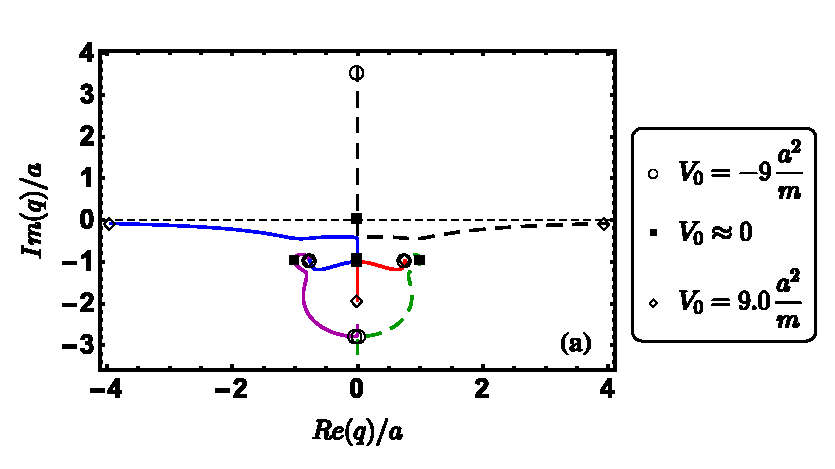
\includegraphics[width=1.0\linewidth]{IVSymEigenvalsVaryingV0new.eps}
    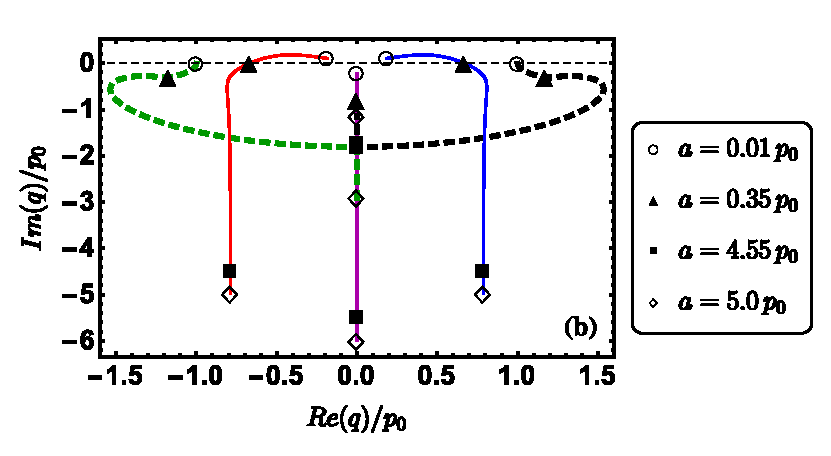
\includegraphics[width=1.0\linewidth]{IVSymEigenvalsVaryinganew.eps}
    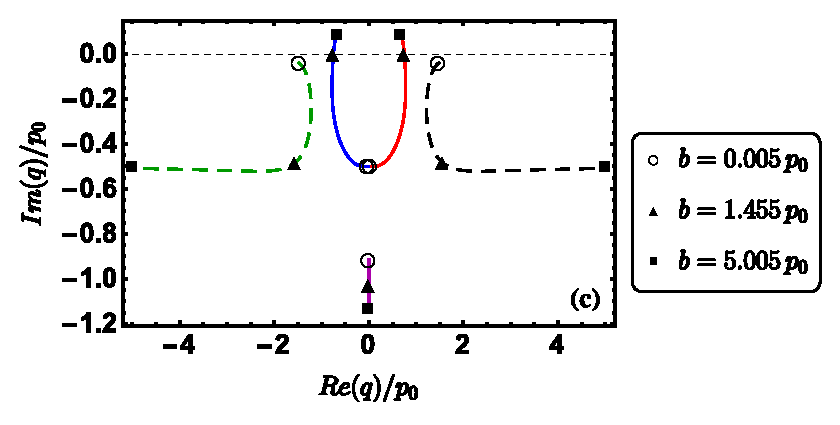
\includegraphics[width=1.0\linewidth]{IVSymEigenvalsVaryingbnew.eps}
    \caption{(Color online) Poles and pole trajectories for the parity pseudohermitian potential \eqref{Ppot} (a) varying $V_0$ with $a=b$; (b) varying $a$ with $b=p_0$, $V_0>0$; (c) varying $b$ with $a=0.5\, p_0$, $V_0>0$.}
    \label{fig:IVSymEigenvals}
\end{figure}



By calculating $Q_{0}$ again explicitly using complex contour integration around the poles at $-q$, $-b-i a$ and $b-i a$, we get that
%
\begin{eqnarray}
&&Q_{0}(q)/m
\nonumber\\
&&=\frac{8 a^2 q^3-4 a^2 q \left(10 a^2+b^2\right)-i a \left(4 a^2+b^2\right)^2+32 i a^3 q^2}{q \left(4 a^2+b^2\right) (a-i q)^2 \left[b^2+(a-i q)^2\right]}.
\nonumber\\
\end{eqnarray}
%
Equation \eqref{roots} has five roots in this case constituting core poles of the $S$ matrix elements.

Figure \ref{fig:IVSymEigenvals} depicts the trajectories of these poles for varying $a$, $b$ or $V_0$. As for the previous potential, the poles are symmetric with respect to the imaginary axis. In Fig. \ref{fig:IVSymEigenvals}(a) there is a single bound state for $V_0<0$ while for positive values there are a resonance/antiresonance pair and a pair of virtual states. There are collisions of eigenvalues for values of $V_0$ close to 0. In Fig. \ref{fig:IVSymEigenvals}(b)  two complex-conjugate (bound) eigenvalues cross the real axis and become a resonance/antiresonance pair. At the exact point where the eigenvalues are on the real axis, the scattering amplitudes diverge, however the eigenvalues of the $S$ matrix do not, since divergences of the left and right amplitudes cancel each other. For $a  \approx 4.55$ $p_0$ a resonance/antiresonance pair collides and becomes a pair of virtual states. In Fig. \ref{fig:IVSymEigenvals}(c) another crossing of the real axis takes place, but in this case when decreasing $b$.

Figure \ref{fig:T_R_fig2} depicts the associated transmission and reflection coefficients as functions of the momentum $p$. The eigenvalues are not always equal since parity pseudohermicity does not imply any strict restriction to them \cite{Ruschhaupt2017}. For large  momenta, i.e. $p \gg \sqrt{2} p_0$, the potential is transparent giving $T^l,T^r \approx 1$. For $p\approx 1.5$ $p_0$ the right incidence transmission has a pronounced peak. Comparing with \ref{fig:IVSymEigenvals}(c), we notice that the values of the potential parameters and the momentum are close to the ones for which the real axis crossing takes place. Around $p = 0.6$ $p_0$ the potential acts as an asymmetric transmitter
%(\red{Use the same code as in the previous paper?:$\mathcal{TR/T,T/A,...}$}) device
\cite{Ruschhaupt2017}.


% Since the potential is separable $S_2 = 1$ (see Appendix \ref{app2}). For $p$ going to infinity there is no scattering and the scattering matrix is the identity.


%%%%%%%%%%%%%%%%%%%%%%%%%%%%%%%%%%%%%%%%%%
%Figure
%%%%%%%%%%%%%%%%%%%%%%%%%%%%%%%%%%%%%%%%%%
\begin{figure}[t]
\begin{center}
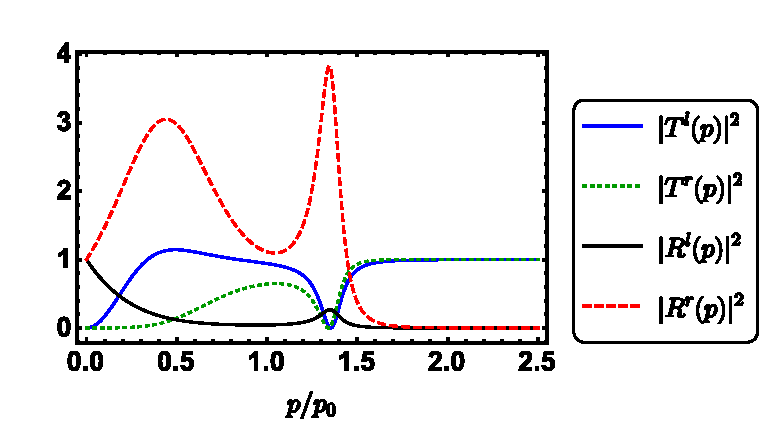
\includegraphics[width=\linewidth]{IVSymTR.eps}
\end{center}
\caption{(Color online) Transmission and reflection coefficients for $a=b=0.5\, p_0$ and $V_0>0$.}
\label{fig:T_R_fig2}
\end{figure}
%%%%%%%%%%%%%%%%%%%%%%%%%%%%%%%%%%%%%%%%%%

%%%%%%%%%%%%%%%%%%%%%%%%%%%%%%%%%%%%%%%%%%
%Figure
%%%%%%%%%%%%%%%%%%%%%%%%%%%%%%%%%%%%%%%%%%

%%%%%%%%%%%%%%%%%%%%%%%%%%%%%%%%%%%%%%%%%%

%\subsection{Symmetry VI example?}
%
%\red{Include other results here}

\section{Conclusion}
\label{sec:RealEigenConclusions}

In this paper we have studied some aspects of the scattering of a structureless particle in one dimension by
generally non-local and non-Hermitian potentials.
%Regarding
%the location of poles of the $S$ matrix eigenvalues in the momentum complex plane,
Conditions that were found for discrete Hamiltonians to imply conjugate pairs of discrete eigenenergies
(pseudohermiticity with respect to a linear operator or commutativity of $H$ with an antilinear operator \cite{Mostafazadeh2002,Mostafazadeh2002a,Mostafazadeh2002b}) can in fact be extended to scattering Hamiltonians in the continuum, implying symmetry relations not just for bound-state eigenvalues
but also for complex
poles of the $S$-matrix. Specifically the poles of $S$ matrix eigenvalues
are symmetrically located with respect to the imaginary axis, also in the lower momentum plane, so that resonances and antiresonance
energies are conjugate pairs as well.
In  terms of the eight possible Hamiltonian symmetries associated with Klein's group of $A$ operators (unity, parity, time reversal and PT)
and their commutation or pseudohermiticity with $H$,
the symmetrical disposition of the poles applies to four of them, which includes hermiticity and PT-symmetry. Potential models
and pole motions are provided for the
two other non trivial symmetries: time-reversal symmetry and parity pseudohermiticity.

The study contributes to deepen our  understanding of asymmetric scattering  (with different responses for left/right incidence) beyond the
much studied  PT-symmetric potentials. This work opens interesting perspectives in AMO physics where much activity on asymmetric-scattering, mostly via optical devices,   is currently being carried out. Moreover asymmetric devices such as rectifiers, Maxwell demons, or diodes will be fundamental to  develop quantum technologies and quantum information. For future work we plan to consider more complicated systems including internal states, as well as physical realizations of the different symmetries in quantum optical systems.

\section{Review of scattering theory formalism \label{sec:ScattFormalism}}
%
A detailed overview of scattering theory can be found in \cite{Taylor1972} and its extension to NH systems in \cite{Muga2004}. Scattering theory describes the interaction of an incoming wave packet with a localized potential. In general, the spectrum of scattering Hamiltonians (as defined at the beginning of section \ref{sec:SymTheory}) has both a discrete part and a continuum with real, positive energies.
%It is precisely this continuous part of the spectrum which is relevant for scattering since the incoming wave packets do not overlap with the eigenstates of the discrete spectrum.
The eigenstates of the continuous spectrum are constructed by the action on plane waves of the M\"oller operators
$\ket{p^\pm}=\Omega_\pm \ket{p}$ and $\ket{\widehat{p}^\pm}=\widehat{\Omega}_\pm \ket{p}$,
where
%onCentral The eigenstates of the continuum may be found by applying are connected to the M\"oller operators, which are defined as
%
\begin{eqnarray}
    \Omega_+ &=& \lim_{t \to -\infty}e^{i H t / \hbar}e^{-i H_0 t/ \hbar},\nonumber\\
    \Omega_- &=& \lim_{t \to \infty}e^{i H^\dagger t/ \hbar}e^{-i H_0 t/ \hbar},\nonumber\\
    \widehat{\Omega}_+ &=& \lim_{t \to -\infty}e^{i H^\dagger t/ \hbar}e^{-i H_0 t/ \hbar},\nonumber\\
    \widehat{\Omega}_- &=& \lim_{t \to \infty}e^{i H t/ \hbar}e^{-i H_0 t/ \hbar},
\end{eqnarray}
%
and a regularization of the limit is implied, see e.g. \cite{Muga2004}.
The M\"oller operators satisfy the isometry relation $\widehat{\Omega}_{\pm}^\dagger\Omega_{\pm} = 1$ and the interwining relations $H \Omega_+ = \Omega_+ H_0$ and $H^\dagger \Omega_- = \Omega_- H_0$.
%The eigenstates of the continuous spectrum are constructed by the action of the M\"oller operators on the eigenstates of momentum operator, .
By using the intertwining relations, it is easy to see that $\ket{p^+}$ and $\ket{\widehat{p}^-}$ are right eigenvectors of $H$ while $\ket{\widehat{p}^+}$ and $\ket{p^-}$ are left eigenvectors of $H$, all with positive energy $E_p = p^2/2m$. In the following we will assume that the Hamiltonian admits a basis of biorthonormal
right/left eigenstates $\left\{ \ket{\psi_n} , \ket{\phi_a} \right\}$ with energies $E_n$ satisfying $\braket{\phi_n}{\psi_m} = \delta_{n,m}$ for the discrete part. The stationary scattering states are also biorthonormal, i.e. $\braket{\widehat{p}^+}{q^+} = \braket{\widehat{p}^-}{q^-} = \delta (p-q)$ and together with the eigenstates of the discrete spectrum they give the resolution of the identity
%
\begin{eqnarray}
    1 &=& \sum_{n}\ketbra{\psi_n}{\phi_n} + \int_{-\infty}^{\infty} dp\, \ketbra{p^+}{\widehat{p}^+}
    \nonumber\\
    &=& \sum_{n}\ketbra{\psi_n}{\phi_n} + \int_{-\infty}^{\infty} dp\, \ketbra{\widehat{p}^-}{p^-}.
    \label{eq:identity}
\end{eqnarray}
%
There is no degeneracy in the discrete spectrum of one-dimensional systems, whereas the continuum is doubly degenerate,
e.g. with continuum eigenfunctions incident from the right or the left.  We shall explicitly make use of this property in what follows. Using the resolution of the identity in terms of discrete eigenstates and the stationary scattering states, the Hamiltonian can be expanded as
%
\begin{equation}
    H = \sum_{n}E_n\ketbra{\psi_n}{\phi_n} + \frac{1}{2m}\int_{-\infty}^{\infty} dp\,p^2 \ketbra{p^+}{\widehat{p}^+}.
    \label{eq:H_Expansion_Continuous}
\end{equation}
%
We call the first and the second terms of \eqref{eq:H_Expansion_Continuous} the discrete, $H_d$, and continuous, $H_c$, parts of the Hamiltonian respectively. A central object is the scattering operator (or matrix), $S \equiv \Omega_-^\dagger \Omega_+$ for scattering processes by $H$ and $\widehat{S} \equiv \widehat{\Omega}_-^\dagger \widehat{\Omega}_+$ for $H^\dagger$. Unhatted quantities refer to scattering by $H$, while hatted ( $\widehat{\;}$ ) quantities refer to scattering by its Hermitian conjugate $H^\dagger$. The scattering operator gives the probability of an incident state $\ket{\psi_{in}}$ to be scattered (by $H$ or $H ^\dagger$) into a state $\ket{\psi_{out}}$ as $\left|\bra{\psi_{out}} S \ket{\psi_{in}}\right|^2$ or $\left|\bra{\psi_{out}} \widehat{S} \ket{\psi_{in}}\right|^2$. Although the scattering operator is not unitary for NH Hamiltonians, $S$ and $\widehat{S}$ obey the generalized unitarity relations $\widehat{S}^\dagger S = S\widehat{S}^\dagger= 1$ which collapses to the usual unitarity condition ($S = \widehat{S}$) if $H = H^\dagger$. If the Hamiltonian is symmetric or pseudohermitian with respect to a linear/antilinear operator $A$, the M\"oller and scattering operators transform according to the intertwining relations in Table \ref{tab:MollerOperatorSyms}. The intertwining relations of the M\"oller operators give the transformation rules for scattering states under $A$ and provide interesting relations between the different transmission/reflection coefficients.

\begin{table}
  \centering
  \begin{tabular}{|c|c|c|}
  \hline
   & \textbf{$A$ linear} & \textbf{$A$ antilinear}

  \\
  \hline

  $A H = H A$
  &
  $
  \begin{array}{ccc}
    &&
    \\
    A \Omega_{\pm}&=&\Omega_{\pm} A
    \\
    A S&=&S A
    \\
    &&
  \end{array}
  $
  &
  $
  \begin{array}{ccc}
    &&
    \\
    A \Omega_{\pm}&=&\widehat{\Omega}_{\mp} A
    \\
    A S&=&\widehat{S}^\dagger A
    \\
    &&
  \end{array}
  $
  \\
  \hline

  $A H = H^\dagger A$
  &
  $
  \begin{array}{ccc}
    &&
    \\
    A \Omega_{\pm}&=&\widehat{\Omega}_{\pm} A
    \\
    A S&=&\widehat{S} A
    \\
    &&
  \end{array}
  $
  &
  $
  \begin{array}{ccc}
    &&
    \\
    A \Omega_{\pm}&=&\Omega_{\mp} A
    \\
    A S&=&S^\dagger A
    \\
    &&
  \end{array}
  $
  \\
  \hline
  \end{tabular}
  \caption{Transformation rules of the M\"oller and scattering operators under
%symmetries/pseudo-symmetries
symmetries with linear or antilinear operators.}
   \label{tab:MollerOperatorSyms}
\end{table}

Also relevant to scattering theory is the transition operator, which is defined as
%
\begin{eqnarray}
T_{op}(E)=V+VG(E)V
\end{eqnarray}
%
where $G(E)=(E-H)^{-1}$ is Green's operator. The transition operator satisfies $T^{\dagger}_{op}(z)=\widehat{T}_{op}(z^*)$ and its matrix elements in momentum representation are related to the  scattering operator by
%
\begin{equation}
    \bra{p} S \ket{p'} = \delta (p-p') -2 i \pi \delta (E_p-E_{p'}) \bra{p}T_{op}(+)\ket{p'},
    \label{eq:SmatrixElements}
\end{equation}
%
where  $T_{op}(\pm)|p'\ra=\lim_{\epsilon\to0^+} T_{op}(E_p\pm i\epsilon)|p'\ra$. This operator can then be used to define the scattering amplitudes
for real $p$ as
%
\begin{eqnarray}\label{art}
R^l(p)&=&-\frac{2\pi im}{p} \la -p|T_{op}({\rm sign}(p))|p\ra\,, \nonumber\\
T^l(p)&=&1-\frac{2\pi im}{p} \la p|T_{op}({\rm sign}(p))|p\ra\,, \nonumber\\
R^r(p)&=&-\frac{2\pi im}{p} \la p|T_{op}({\rm sign}(p))|-p\ra\,, \nonumber\\
T^r(p)&=&1-\frac{2\pi im}{p} \la -p|T_{op}({\rm sign}(p))|-p\ra,
\end{eqnarray}
%
where $R^{l,r}$ is the left/right reflection amplitude and $T^{l,r}$ is the left/right transmission amplitude. We assume that the amplitudes admit analytic continuations. The generalized unitarity relation of the scattering operators give the following set of equations for the amplitudes
%
\begin{eqnarray}
    \widehat T^l(p) T^{l*}(p) + \widehat R^l(p) R^{l*}(p) &=& 1,
    \nonumber\\
    \widehat T^r(p) T^{r*}(p) + \widehat R^r(p) R^{r*}(p) &=& 1,
    \nonumber\\
    \hat T^{l*}(p) R^r(p) + T^r(p) \widehat R^{l*}(p) &=& 0,
    \nonumber\\
    T^l(p) \widehat R^{r*}(p) + \widehat T^{r*}(p) R^l(p) &=& 0,
    \label{gurAmplitudes}
\end{eqnarray}
%
where $p$ is taken to be real and nonnegative. The Dirac deltas in Eq. \eqref{eq:SmatrixElements} make clear that the $S$ matrix only connects momentum eigenstates having the same kinetic energy. Factoring out the Dirac delta of energy using $\delta(p-p') = \frac{|p|}{m}\delta(E_p-E_{p'})\delta_{pp'}$ ($\delta_{pp'}$ is to be understood as a Kronecker delta of the signs of the momenta) we can write $\bra{p} S \ket{p'} = \frac{|p|}{m}\delta(E_p-E_{p'})\bra{\mathbf{p}} \mathsf{S} \ket{\mathbf{p'}}$ in terms of the two-dimensional vectors $\ket{\mathbf{p}}\equiv (1,0)^T$ and $\ket{-\mathbf{p}}\equiv (0,1)^T$ that correspond to the states $\ket{p}$ and $\ket{-p}$ for $p > 0$
\cite{Muga2004}. The previous relation defines the on-the-energy-shell $\mathsf{S}$ matrix as
%
\begin{eqnarray}
  \bra{\mathbf{p}} \mathsf{S} \ket{\mathbf{p'}} &=& \delta_{pp'} - \frac{2i\pi m}{|p|} \la p|T_{op}(+)|p'\ra \nonumber \\
  & \Downarrow & \\
  \mathsf{S} &=&
  \left(
  \begin{array}{cc}
    T^l(p)&R^r(p)
    \\
    R^l(p)&T^r(p)
  \end{array}
  \right)\nonumber.
\end{eqnarray}
%
$\mathsf{\widehat{S}}$ can be defined similarly. The on-the-energy-shell scattering matrix $\mathsf{S}$ inherits the generalized unitarity relation of the scattering operator $S$, i.e., $\mathsf{\widehat{S}}^\dagger\mathsf{S} = \mathsf{1}$. Equation \eqref{gurAmplitudes} is just this generalized unitarity relation written for all matrix elements.



%
%\section{Symmetries for real or conjugate pairs of eigenvalues}
%\label{app4}
%
%The symmetries which admit real or complex conjugate pairs of eigenvalues are II, IV,V and VII. These conditions have been previously discussed in \red{CITE ALI AND BENDER HERE} and can be heuristically understood in some cases as follows. Symmetry II is simply Hermiticity. Symmetry V implies that the Hamiltonian must be real which would lead to a real characteristic polynomial (which must have complex conjugate roots \red{cite}). Symmetry VII is PT symmetry which is well discussed in the literature as having complex conjugate pairs of eigenvalues \red{cite}.
%
%In this section we will provide a brief overview of why this occurs. From Appendix \ref{app5}, we can see that all these symmetries can be written as $AH=HA$ for $A$ anti-linear. From this we get that
%%
%\begin{eqnarray}
%H A \ket{E_j}&=&A H \ket{E_j} \nonumber \\
%				   &=&E_{j}^{*} A \ket{E_j}.
%\end{eqnarray}
%%
%Hence all the eigenvalues are complex conjugate pairs in this case. In particular when $A \ket{E_j}=\ket{E_j}$ we get that $E_j \in \mathbb{R}$.
%
%
%
\section{Alternative formulation of $A$-pseudohermitian symmetries as ordinary (commuting) symmetries}
\label{app5}
%
%
%
Symmetry relations like \eqref{gs2} (for $A$ either linear or antilinear) may also be expressed as ordinary (commuting) symmetries, generalizing for scattering Hamiltonians the work in \cite{Mostafazadeh2002,Mostafazadeh2002a,Mostafazadeh2002b}. In other words, for a Hamiltonian $H$ and a linear hermitian (antilinear hermitian) operator $A$ satisfying \eqref{gs2} we can find an antilinear (linear) operator $B$ that commutes with $H$. In this appendix we explicitly construct the operators $B$ from the Hamiltonian both for $A$ linear and antilinear in the first and second sections respectively.

Let us assume for now that besides $A$ (linear or antilinear) there exists an invertible and hermitian antilinear operator $\tau$ that also satisfies \eqref{gs2}. With $A$ and $\tau$ let us define the operator $B = A^{-1} \tau$ that will be antilinear (linear) for $A$ linear (antilinear). As defined, $B$ commutes with the Hamiltonian, because
%
\begin{eqnarray}
    B H &=& A^{-1}\tau H \nonumber \\
           &=& A^{-1} H^\dagger \tau \nonumber \\
           &=& H A^{-1} \tau\nonumber \\
           &=& H B.
    \label{eq:HiddenSymmetry}
\end{eqnarray}
%
%so $B$ represents a symmetry of the Hamiltonian in the usual sense.
$B$ is not generally Hermitian unless $\tau$ commutes with $A^{-1}$.
%This connection between symmetry and pseudo hermiticity  justifies taking into account equations like \eqref{gs2} since they can be translated to the usual symmetry equations implemented by commutations.

The main task  to define  $B$ is to find the antilinear operator $\tau$ that satisfies \eqref{gs2}.
This can be achieved if the eigenvectors of the Hamiltonian and its adjoint form bases of the Hilbert space that are biorthonormal.
In \cite{Mostafazadeh2002b} the expression of $\tau$ for a discrete spectrum (with no degeneracy) is found as
%
\begin{equation}
    \tau_d \ket{\zeta} = \sum_n \braket{\zeta}{\phi_n} \ket{\phi_n},
    \label{eq:GenericTau}
\end{equation}
%
where the $d$ subscript indicates that the Hamiltonian has a discrete spectrum. The action of the operator in Eq. \eqref{eq:GenericTau} on a vector in an eigenspace amounts to complex conjugation of its coordinate
representation. $\tau_d$ is clearly antilinear, Hermitian (for antilinear operators hermicity is defined as $\braket{\chi}{\tau_d \zeta} = \braket{\zeta}{\tau_d \chi}$), and invertible. It can be checked that the relation $\tau_d H = H^\dagger \tau_d$ is satisfied.

To generalize this to Hamiltonians whose spectrum includes a continuous part, we have to build an antilinear operator $\tau$ that acts in both the subspaces, ${\cal H}_d$ and ${\cal H}_c$, that are respectively spanned by the eigenfunctions associated with the discrete (point) and continuous spectra of the Hamiltonian. We propose to take $\tau= \tau_d + \tau_c$. The operators $\tau_d$ and $\tau_c$ act on complementary subspaces of the Hilbert space: while $\tau_d$ maps ${\cal H}_d$ to ${\cal H}_d$ and annihilates states in ${\cal H}_c$,   $\tau_c$ maps ${\cal H}_c$ to ${\cal H}_c$ and annihilates states in ${\cal H}_d$.
%endred
Specifically, we take $\tau_d$ to be given by Eq. (\ref{eq:GenericTau}) with  $n$ denoting the eigenvectors of the Hamiltonian associated with the discrete part of the spectrum. To construct $\tau_c$, note that to satisfy $\tau H = H^\dagger \tau$ (Eq. \eqref{gs2}) it has to transform right scattering eigenvectors into some linear combination of left scattering eigenvectors in the same energy shell. This is so because
%
% \begin{eqnarray}
%     H^\dagger \tau \ket{p^+} &=& \tau H \ket{p^+}\nonumber\\
%     &=& \tau E_p\ket{p^+}\nonumber\\
%     &=& E_p \tau \ket{p^+}.
% \end{eqnarray}
\begin{equation}
    H^\dagger \tau \ket{p^+} = \tau H \ket{p^+}
    = \tau E_p\ket{p^+}
    = E_p \tau \ket{p^+}.
\end{equation}
%
To fulfill the last requirement we set
%
\begin{equation}
    \tau_c \ket{\zeta} = \int_{-\infty}^{\infty}\!\! dp  \left[ C_+(p) \braket{\zeta}{\widehat{p}^+}\ket{\widehat{p}^+} + C_-(p)\braket{\zeta}{\widehat{p}^+}\ket{-\widehat{p}^+} \right],
    \label{eq:ContinuousTau}
\end{equation}
%
where $C_+(p)$ and $C_-(p)$ are complex coefficients. It is straightforward to check that $\tau_c \ket{p^+} = C_+(p)\ket{\widehat{p}^+} + C_-(p)\ket{-\widehat{p}^+}$.
%, which is a left scattering vector with energy $E_p$.
The operator in \eqref{eq:ContinuousTau} is clearly antilinear because of the antilinearity of the inner product with respect to its first argument. Hermicity of $\tau$ requires $C_-(p) = C_-(-p)$. The condition that $\tau$ must be invertible restricts the coefficients in Eq. (\ref{eq:ContinuousTau}) further.
Consider the \textit{on shell} representation of $\tau_c$, $\braket{p^+}{\tau q^+} = \frac{|p|}{m}\delta(E_p-E_q) \mathsf{C}_{p,q}$, with $\mathsf{C}_{p,q} \equiv \delta_{p,q} C_+(q) + \delta_{p,-q} C_-(q)$, or in matrix form
%
\begin{equation}
\mathsf{C}(p)=
    \begin{pmatrix}
    C_+(p) & C_-(p) \\
    C_-(p) & C_+(-p)
    \end{pmatrix}.
\end{equation}
%
Since $\tau$ has to be invertible, $\mathsf{C}(p)$ must be invertible as well. This implies  $C_+(p)C_+(-p) - C_-(p)C_-(p) \neq 0$.

In the following sections we construct expressions for $B$, in section 1 for $A$ linear, and in section 2 for $A$ antilinear.
% on the continuum.

\subsection{Pseudohermicity with linear operators\label{ContPseudoHermicity}}
%
In \cite{Mostafazadeh2002,Mostafazadeh2002a,Mostafazadeh2002b} it is shown that pseudohermitian Hamiltonians, i.e. those satisfying \eqref{gs2} for $A=\eta$ with $\eta$ a hermitian and invertible linear operator, posses an energy spectrum whose complex eigenvalues come in complex-conjugate pairs. Moreover the eigenspaces associated with  the eigenvalues $E$ and $E^*$ have the same degeneracy and $\eta$ maps one to the other. Conversely, if the complex part of the spectrum of $H$ contains only complex-conjugate pairs, it can be shown that there exists an $\eta$ for which the Hamiltonian satisfies \eqref{gs2}.
These results hold for a general class of diagonalizable Hamiltonians with a discrete spectrum. For these Hamiltonians we can identify $\eta$ with
%For discrete Hamiltonians with complex-conjugated pairs the operator satisfying \eqref{gs2} is
%
\begin{equation}
    \begin{split}
    \eta_{d} &= \sum_{n_0} \ketbra{\phi_{n_0}}{\phi_{n_0}}\\ &+ \sum_n \Big[\ketbra{\phi_{n_-}}{\phi_{n_+}} +  \ketbra{\phi_{n_+}}{\phi_{n_-}}\Big],
    \end{split}
    \label{eq:DiscreteEta}
\end{equation}
%
% Consider a discrete Hamiltonian having the complex part of the spectrum in conjugate pairs and no degeneracy, then it can be expanded as
%
% \begin{widetext}
% \begin{equation}
%     H_d = \sum_{n_0}E_{n_0} \ketbra{\psi_{n_0}}{\phi_{n_0}} + \sum_n\Big[E_{n_+} \ketbra{\psi_{n_+}}{\phi_{n_+}} + E_{n_+}^* \ketbra{\psi_{n_-}}{\phi_{n_-}}\Big],
% \end{equation}
% \end{widetext}
%
where the states $\ket{\psi_{n_0}}$ ($\ket{\phi_{n_0}}$) correspond to the right (left) eigenstates of $H$ with real energy $E_{n_0}$.
$\ket{\psi_{n+/n-}}$  (respectively $\ket{\phi_{n+/n-}}$) correspond to the right (respectively left) eigenvectors whose eigenvalue $E_{n+/n-}$  has a positive/negative imaginary part.
This gives $\eta_d \ket{\psi_{n_0}} = \ket{\phi_{n_0}}$, $\eta_d\ket{\psi_{n_+}} = \ket{\phi_{n_-}}$ and $\eta_d\ket{\psi_{n_-}} = \ket{\phi_{n_+}}$. Clearly $\eta_d$ is compatible with pseudohermicity since it maps right eigenvectors associated with the eigenvalue $E$ into left eigenvectors with eigenvalue $E^*$ and the pseudohermicity relation \eqref{gs2} is satisfied. To generalize \eqref{eq:DiscreteEta} for a scattering Hamiltonian we must add an additional term $\eta_c$ which acts on the subspace of scattering states and is compatible with the hermiticity and invertibility of $\eta = \eta_d + \eta_c$. Since $\eta$ should transform the right scattering states into left ones in the same energy shell, $\eta_c \ket{p^+}$ should be a linear combination of both $\ket{\widehat{p}^+}$ and $\ket{-\widehat{p}^+}$. Accordingly, we propose
%
\begin{equation}
    \eta_c = \int_{-\infty}^\infty dp\; \left[\Lambda_+(p)\ketbra{\widehat{p}^+}{\widehat{p}^+} + \Lambda_-(p)\ketbra{-\widehat{p}^+}{\widehat{p}^+}\right],
    \label{eq:EtaContinuousPart}
\end{equation}
%
where $\Lambda_+(p), \Lambda_-(p)$ are complex coefficients depending on the momentum $p$. Hermicity of $\eta$ requires $\Lambda_+(p) \in \mathbb{R}$ and $\Lambda_-^*(p) =\Lambda_-(-p)$.

Since $\eta_c$ connects scattering states with the same energy it admits the following \textit{on-shell} representation, $\bra{q^+}\eta_c\ket{p^+} = \frac{|p|}{m}\delta(E_q-E_p) \mathsf{\Lambda}_{q,p}(p)$, with $\mathsf{\Lambda}_{q,p}(p) \equiv \delta_{q,p} \Lambda_+(p) + \delta_{q,-p} \Lambda_-(p)$, or in matrix form
%
\begin{equation}
    \mathsf{\Lambda}(p)
    =
    \left(
    \begin{matrix}
        \Lambda_+(p) & \Lambda_-^*(p) \\
        \Lambda_-(p) & \Lambda_+(-p)
    \end{matrix}
    \right).
    \label{eq:onShellEtaContinuous}
\end{equation}
%
%where we have used the hermicity condition for the $\Lambda_-(p)$ coefficients.
Since $\eta$ has to be invertible, this implies that the determinant of $\mathsf{A}(p)$ should not vanish i.e. $\Lambda_+(p) \Lambda_+(-p) - \Lambda_-(p) \Lambda_-^*(p) \neq 0$. The inverse of $\eta$ is then $\eta^{-1} = \eta_d^{-1} + \eta_c^{-1}$ with
%
\begin{equation}
  \begin{split}
  \eta_d^{-1} &= \sum_{n_0} \ketbra{\psi_{n_0}}{\psi_{n_0}}\\
  &+\sum_{n} \left[\ketbra{\psi_{n_+}}{\psi_{n_-}} + \ketbra{\psi_{n_-}}{\psi_{n_+}}\right]
\end{split}
\end{equation}
%
\begin{equation}
    \eta_c^{-1} = \int_{-\infty}^\infty dp\; \left[\Lambda_+^{(-1)}(p)\ketbra{p^+}{p^+} + \Lambda_-^{(-1)}(p)\ketbra{-p^+}{p^+}\right],
\end{equation}
%
where the complex coefficients $\Lambda_\pm^{(-1)}(p)$ are taken from the inverse of $\mathsf{\Lambda}(p)$
%
\begin{equation}
  \mathsf{\Lambda}^{-1}(p)
  =
  \left(
  \begin{matrix}
      \Lambda_+^{(-1)}(p) & \Lambda_-^{(-1)*}(p) \\
      \Lambda_-^{(-1)}(p) & \Lambda_+^{(-1)}(-p)
  \end{matrix}
  \right).
  \label{eq:onShellEtaContinuous2}
\end{equation}
%
Using the orthogonality between the subspace of discrete (bound) and scattering states we find the final expression for $B$
%
\begin{eqnarray}
%  \begin{split}
  &&B\ket{\zeta} = \eta_d^{-1}\tau_d\ket{\zeta}+  \eta_c^{-1}\tau_c\ket{\zeta}\nonumber\\
  &&=\sum_{n_0}\braket{\zeta}{\phi_{n_0}}\ket{\psi_{n_0}}
  %\nonumber\\
  +\sum_{n}\braket{\zeta}{\phi_{n_+}}\ket{\psi_{n_-}}
  %\nonumber\\
  +\sum_{n}\braket{\zeta}{\phi_{n_-}}\ket{\psi_{n_+}}\nonumber\\
  &&+\int_{-\infty}^{\infty}dp\,\braket{\zeta}{\widehat{p}^+}
  \left[ \tilde{C}_+(p)\ket{p^+} + \tilde{C}_-(p)\ket{-p^+} \right],\nonumber\\
%  \end{split}
\end{eqnarray}
%
with $\tilde{C}_\pm(p) = C_+(p)\Lambda_\pm^{(-1)}(p)+C_-(p)\Lambda_\mp^{(-1)}(-p)$. Note that the resulting operator $B$ is antilinear.

\subsection{Pseudohermicity with antilinear operators}
%repeated in main text
%This symmetry relation implies that if $\ket{\psi}$ is a right eigenvector of $H$ with eigenvalue $E$, $A \ket{\psi}$ will be a left eigenvector with the same energy since $H \da A \ket{\psi} = A H \ket{\psi} = E^* A \ket{\psi}$.

In this section we will consider the case where the operator $A$ appearing in Eq. (\ref{gs2}) is antilinear.  In ref. \cite{Mostafazadeh2002b} this is called antipseudohermicity, but we will not use this terminology in order to avoid confusion with antihermicity ($H = - H^\dagger$). The effect of $A$ on a right eigenvector of $H$ is to transform it  into its corresponding biorthonormal partner, i.e. the left eigenvector corresponding to the same energy
%
% \begin{eqnarray}
%     H^\dagger A \ket{\psi_n} &=& A H \ket{\psi_n}\nonumber\\
%     &=& A E_n\ket{\psi_n}\nonumber\\
%     &=& E_n^* A \ket{\psi_n}\nonumber\\
%     &\big\Downarrow&\nonumber\\
%     A\ket{\psi_n}&\propto&\ket{\phi_n}.
% \end{eqnarray}
\begin{eqnarray}
    H^\dagger A \ket{\psi_n} = A H \ket{\psi_n}
    &=&A E_n\ket{\psi_n}
    = E_n^* A \ket{\psi_n}\nonumber\\
    &\big\Downarrow&\nonumber\\
    A\ket{\psi_n}&\propto&\ket{\phi_n}.
\end{eqnarray}
%
$A$ also admits a decomposition similar to Eq. \eqref{eq:GenericTau}.
The Hamiltonian satisfies Eq. (\ref{gs2})
with respect to $\tau$. One can check that $A^{-1}\tau$ is a linear symmetry of the Hamiltonian,
$HA^{-1}\tau - A^{-1}\tau H=0$. The expansion of $A$ on the discrete and scattering basis is
%
\begin{equation}
    A \ket{\xi} = \sum_n g_n \braket{\xi}{\phi_n} \ket{\phi_n} + \int dp \;  \braket{\xi}{\widehat{p}^+}   \left[ G_+(p) \ket{\widehat{p}^+} + G_-(p)\ket{-\widehat{p}^+} \right],
\end{equation}
%
with $A\ket{p^+\!}\!=\!G_+(p)\ket{\widehat{p}^+\!}+G_-(p)\ket{\!-\!\widehat{p}^+\!}$ and  $g_n = \bra{\psi_n}A {\psi_n}\ra$.
As examples we have found the expressions of $B = A^{-1}\tau$ for $A_T = \Theta$(time reversal) and $A_{PT} = \Pi\Theta$ (PT). In both cases we have $A_T^{-1}=A_T$ and $A_{PT}^{-1}=A_{PT}$.
%
\subsubsection{PT Symmetry}
The action of $B_{PT} = A_{PT}\tau$ on an arbitrary state is
%
\begin{equation}
    B_{PT}\ket{\zeta} = A_{PT}\tau\ket{\zeta}
                                   = A_{PT} \left\{ \sum_n \braket{\zeta}{\phi_n} \ket{\phi_n} + \int dp\; \left[ C_+(p) \braket{\zeta}{\widehat{p}^+}\ket{\widehat{p}^+} + C_-(p)\braket{\zeta}{\widehat{p}^+}\ket{-\widehat{p}^+} \right] \right\}.
\end{equation}
%
~\\
~\\
~\\
~\\
~\\
~\\
Using $A_{PT} H = H^\dagger A_{PT}$ and table \ref{tab:MollerOperatorSyms} we have $A_{PT} \ket{\widehat{p}^\pm} = \ket{\widehat{p}^\mp}$. Note that The ``-" right scattering states can be expressed in terms of the ``+" right scattering states as
%
\begin{eqnarray}
    \ket{\widehat{p}^-} &=& \int dq\; \ket{q^+}\braket{\widehat{q}^+}{\widehat{p}^-}\nonumber\\
    &=& \int dq\; \ket{q^+}\bra{q}\widehat{\Omega}_+^\dagger \widehat{\Omega}_- \ket{p}\nonumber\\
    &=& \int dq\; \ket{q^+}\bra{q} \widehat{S}^\dagger \ket{p}\nonumber\\
    &=& \ket{p^+}\bra{p} \widehat{\mathsf{S}}^\dagger \ket{p} + \ket{-p^+}\bra{-p} \widehat{\mathsf{S}}^\dagger \ket{p}.
\end{eqnarray}
% \begin{eqnarray}
%   \ket{\widehat{p}^-} = \int dq\; \ket{q^+}\braket{\widehat{q}^+}{\widehat{p}^-}
%   = \int dq\; \ket{q^+}\bra{q}\widehat{\Omega}_+^\dagger \widehat{\Omega}_- \ket{p}\nonumber\\
%
%   = \int dq\; \ket{q^+}\bra{q} \widehat{S}^\dagger \ket{p}
%   = \ket{p^+}\bra{p} \widehat{\mathsf{S}}^\dagger \ket{p} + \ket{-p^+}\bra{-p} \widehat{\mathsf{S}}^\dagger \ket{p}.
% \end{eqnarray}
%
~\\~\\
With all this, the final form of $B_{PT}$ is
%
\begin{eqnarray}
    B_{PT} &=&   \sum_n (g_n^*)^{-1} \ketbra{\psi_n}{\phi_n} \nonumber \\
                &+& \int dp\; \left[ \tilde{C}_+^*(p)\ketbra{p^+}{\widehat{p}^+} + \tilde{C}_-^*(p)\ketbra{-p^+}{\widehat{p}^+} \right], \nonumber \\
\label{C13}
\end{eqnarray}

%\begin{widetext}
%\begin{equation}
%    B_{PT}=   \sum_n (g_n^*)^{-1} \ketbra{\psi_n}{\phi_n} +\int dp\; \left[ \tilde{C}_+^*(p)\ketbra{p^+}{\widehat{p}^+} + \tilde{C}_-^*(p)\ketbra{-p^+}{\widehat{p}^+} \right],
%\end{equation}
%\end{widetext}
%
with $C_{\pm}^*(p) = C_{\pm}^*(p) \bra{\pm p} \widehat{\mathsf{S}}^\dagger \ket{\pm p} + C_{\mp}^*(p) \bra{\pm p} \widehat{\mathsf{S}}^\dagger \ket{\mp p}$.

\subsubsection{Time-Reversal Symmetry}
%
For time-reversal symmetry,
%
\begin{equation}
    B_{T}\ket{\zeta} = A_{T}\tau\ket{\zeta} = A_{T} \left\{ \sum_n  \braket{\zeta}{\phi_n} \ket{\phi_n} + \int dp\; \left[ C_+(p) \braket{\zeta}{\widehat{p}^+}\ket{\widehat{p}^+} + C_-(p)\braket{\zeta}{\widehat{p}^+}\ket{-\widehat{p}^+} \right] \right\}.
\end{equation}
%
Since the time-reversal operator satisfies the relation \eqref{gs2} with the Hamiltonian, Table \ref{tab:MollerOperatorSyms} implies $A_T\ket{\widehat{p}^\pm} = \ket{-\widehat{p}^\mp}$. The linear symmetry operator can be expressed as in Eq. (\ref{C13}) but in this case $\tilde{C}_{\pm}^*(p) = C_{\pm}^*(p) \bra{\pm p} \widehat{\mathsf{S}}^\dagger \ket{\mp p} + C_{\mp}^*(p) \bra{\pm p} \widehat{\mathsf{S}}^\dagger \ket{\pm p}$.

%\section{Spectrum of Non-Hermitian Hamiltonians}
%\label{sec:ConjugatePairs}
%
%%\blue{\textbf{Include a possible result about reality of the spectrum}}. Let $H$ be a N-H Hamiltonian which is invariant under the action of some antilinear superoperator $\cal{L}$, i.e., $\mathcal{L}\left(H\right) = H$. By definitiossn, an antilinear operator satisfies $\mathcal{L}\left(\alpha H_1 + \beta H_2\right)= \alpha^*\mathcal{L}\left(H_1\right) + \beta^*\mathcal{L}\left(H_2\right)$. From now on, we assume the existence of a biorthonomal basis associated with the hamiltonian $H$. The biorthonomal basis is build with the right and left eigenvectors of $H$ defined by the eigenvalue identities $H \ket{\psi_n} = E_n \ket{\psi_n}$ and $\bra{\phi_n} H =\bra{\phi_n} E_n$. The biorthonomal basis satisfy
%%
%\begin{eqnarray}
%    \braket{\phi_n}{\psi_m} &=& \delta_{n,m}\nonumber\\
%    \sum_n \ket{\psi_n}\bra{\phi_n} &=& \sum_n \ket{\phi_n}\bra{\psi_n} = 1.
%    \label{eq:biortSyst}
%\end{eqnarray}
%%
%The biorthonomal system allows us to define a set of operators $\Lambda_{n,m} \equiv \ket{\psi_n}\bra{\phi_m}$. The operators $\Lambda_{n,m}$ have a few nice properties that can be useful later.
%
%\begin{enumerate}
%  \item They satisty $\Lambda_{n_1,m_1}\Lambda_{n_2,m_2} = \delta_{n_2,m_1}\Lambda_{n_1,m_2}$ and the orthogonality relation $\Sbraket{\Lambda_{n_1,m_1}^\dagger}{\Lambda_{n_2,m_2}} = \delta_{n_1,m_2}\delta_{n_2,m_1}$
%
%  \item They are linearly independent of each other (kind of obvious).
%
%  \item  The first and second properties imply that the $\Lambda_{n,m}$ are a basis of the vector space of the linear operators on the Hilbert space $\mathcal{H}$. So, for every linear operator acting on $\mathcal{H}$ we have $A = \sum_{n,m}A_{n,m}\Lambda_{n,m}$ with $A_{n,m} = \Sbraket{\Lambda_{m,n}^\dagger}{A}$.
%\end{enumerate}
%%
%%
%\begin{eqnarray}
%    \sum_n E_n \Lambda_{n,n} &=& \sum_n E_n^* \mathcal{L}\left(\Lambda_{n,n}\right),\nonumber\\
%    &\Rightarrow&
%    \begin{cases}
%        \sum_n E_n^* \Sbraket{\Lambda_{m,m}^\dagger}{\mathcal{L}\left(\Lambda_{n,n}\right)} = E_m\\
%        \sum_n E_n^* \Sbraket{\Lambda_{p,m}^\dagger}{\mathcal{L}\left(\Lambda_{n,n}\right)} = 0,m\neq p
%    \end{cases}
%    \nonumber\\
%\end{eqnarray}
%%
%\blue{It would be nice if we could prove $\Sbraket{\Lambda_{m,m}^\dagger}{\mathcal{L}\left(\Lambda_{n,n}\right)} = \delta_{n,p}$. This would imply that the eigenenergies are real or come in complex conjugate pairs.}


%
%
%The symmetries which admit real or complex conjugate pairs of eigenvalues are II, IV,V and VII. Here we will briefly outline the conditions for this.\red{Related to Ali paper. Cite here}
%
%%First consider the symmetries II and IV which have the relation $AH=H^{\dagger}A$ for $A$ linear. We start with the eigenvalue equation,
%%%
%%\begin{eqnarray}
%%H \ket{\psi_E}=E \ket{\psi_E}
%%\end{eqnarray}
%%%
%%If we then apply $A$ to both sides we get
%%%
%%\begin{eqnarray}
%%AH|\ra A\psi_E\ra =E|A\psi_E\ra =H^\dagger |A\psi_E.
%%%(E^{*}_i-E_j)\bra{E_i}A\ket{E_j}=0. \label{cc_pair_rule}
%%\end{eqnarray}
%%%
%%The ``bra'' version of the last equality is $\la A\psi_E|H=\la A\psi_E|E^*$, which shows that eigenvalues of $H$ come in
%%conjugate pairs (or are real). For unbroken symmetry, i.e., if $|A\psi_E\ra=|\psi_E\ra$ up to a phase factor, then $E$ is real.
%%This is always fulfilled
%%for symmetry II  (Hermiticity) since $A=1$.
%
%%\red{comment on what domains might Klein group operators be positive?}
%
%\red{This proof known in some Bender paper. Cite here}%\\
%
%Next we consider symmetries V and VII given by $AH=HA$ for $A$ anti-linear. From this we get that
%%
%\begin{eqnarray}
%H A \ket{E_j}&=&A H \ket{E_j} \nonumber \\
%				   &=&E_{j}^{*} A \ket{E_j}.
%\end{eqnarray}
%%
%Hence all the eigenvalues are complex conjugate pairs in this case. In particular when $A \ket{E_j}=\ket{E_j}$ we get that $E_j \in \mathbb{R}$.
%
%Symmetry V implies that the Hamiltonian must be real which would lead to a real characteristic polynomial (which must have complex conjugate roots \red{cite}). Symmetry VII is PT symmetry which is well discussed in the literature as having complex conjugate pairs of eigenvalues \red{cite}.


\section{Properties of separable potentials}
%\section{Transition operator for a separable potential}
\subsection{Transition operator}
\label{app1}
%%%%%%%%%%%%%%%%%
 For a separable potential $V=V_0 \ketbra{\phi}{\chi}$, the transition operator becomes
\begin{eqnarray}
T_{op}=\alpha \ketbra{\phi}{\chi}
\end{eqnarray}
where $\alpha=V_{0}+V_{0}^{2}\bra{\chi}G(E)\ket{\phi}$. Then using the Lippmann-Schwinger equation we get that
%
\begin{eqnarray}
T_{op}(E)&=&V+VG_{0}(E)T_{op}(E)
\nonumber \\
&=& \left[V_{0}+\alpha V_{0} \bra{\chi}G_{0}(E)\ket{\phi}\right]\ketbra{\phi}{\chi}
\end{eqnarray}
%
where $G_{0}(E)=(E-H_{0})^{-1}$ is the Green's operator for free motion. Solving for $\alpha$ now gives
%
\begin{eqnarray}
\alpha =\frac{V_{0}}{1-V_{0} \bra{\chi}G_{0}(E)\ket{\phi}}
		   =\frac{V_{0}}{1-V_{0} Q_{0}(E)}.
\end{eqnarray}
%
%%%%%%%%%%%%%%%%%
%
%
%
%
\subsection{$S$-matrix eigenvalues}
\label{app2}
%
%
%
%
The eigenvalues for the S-matrix are given by Eq. \eqref{Sform} in terms of the reflection and transmission amplitudes. For a separable potential, using Eq. \eqref{art}, we can simplify the transmission and reflection coefficients as
\begin{eqnarray}
T^{l}&=&1-\frac{2 \pi i m}{p} \alpha \phi(p) \chi^{*}(p),
\nonumber \\
T^{r}&=&1-\frac{2 \pi i m}{p} \alpha \phi(-p) \chi^{*}(-p),
\nonumber \\
R^{l}&=&-\frac{2 \pi i m}{p} \alpha \phi(-p) \chi^{*}(p),
\nonumber \\
R^{r}&=&-\frac{2 \pi i m}{p} \alpha \phi(p) \chi^{*}(-p).
\nonumber \\
\end{eqnarray}
%
If we now define
%
\begin{equation}
\Gamma=\frac{2 \pi i m}{p} \alpha \left[\phi(p) \chi^{*}(p)+\phi(-p) \chi^{*}(-p)\right],
\end{equation}
%
we can write the eigenvalues as simply
%
\begin{eqnarray}
S_{j}&=&1-\frac{\Gamma-(-1)^{j}\Gamma}{2}.
\end{eqnarray}
%
Note that $S_2=1$ for all $p$. Clearly the following relation must also always hold for the reflection and transmission amplitudes,
%
\begin{equation}
T^l + T^r - T^l T^r + R^l R^r = 1.
\end{equation}
%
%
%
%
%
%
%
%
\subsection{Uniqueness of bound state}
\label{app3}
%
A separable potential  can only have at most one bound state $\ket{\psi_{E}}$.
In momentum representation,
%
\begin{eqnarray}
\braket{p}{\psi_{E}}&=&\bra{p}\frac{V_{0}}{E-H_{0}}\ket{\phi}\braket{\chi}{\psi_{E}}
\nonumber \\
&=&\frac{M}{p^{2}-q_{B}^{2}}\braket{p}{\phi},
\end{eqnarray}
%
where $M=-2 m V_{0} \braket{\chi}{\psi_{E}}$ and $q_{B}^2=2 m E<0$. Suppose there is a second bound state $\ket{\psi_{E'}}$,
with corresponding quantities $M'$ and $q_{B'}^2$. Then,
%
\begin{eqnarray}
\braket{\psi_{E'}}{\psi_{E}}&=&M M' \int_{-\infty}^\infty dp \left|\braket{p}{\phi}\right| \frac{1}{p^{2}-q_{B}^{2}}\frac{1}{p^{2}-q_{B'}^{2}}. \nonumber \\		\end{eqnarray}
%
Since $MM'\ne 0$ and the integral is positive the overlap cannot be zero
so there cannot be two bound states.
         %complex plane symmetries of nh Hamiltonians
  % %!TEX root = ../Thesis.tex
%Chapter 1

\chapter{Symmetries of ($N\times N$) non-Hermitian Hamiltonian matrices}
\label{ChapterNNSymmetries}
\lhead{Chapter NxN. \emph{Symmetries of ($N\times N$) non-Hermitian Hamiltonian matrices}} % Write in your own chapter title to set the page header
%
A non-Abelian group of sixteen symmetry operations on (generally) \linebreak non-Hermitian
discrete Hamiltonians represented by $N\times N$ matrices is studied. The symmetry operations are described by unitary/antiunitary superoperators that arise  when combining
three basic generating operations with simple ``geometric'' interpretations. The corresponding Hamiltonian symmetries occur when
the Hamiltonian remains invariant under the superoperator action. These symmetries  include PT-symmetry and hermiticity as particular cases.
The interplay between the group of symmetry operations and Hamiltonian symmetries
is analyzed systematically by introducing the concepts of equivalent operations and associated symmetries.
Spectral properties implied by some of the symmetries are described.
%
\newpage
%
\section{Introduction}
%
Non Hermitian Hamiltonians have been used for a long time in nuclear, atomic, and molecular physics
as effective interactions, and have become common in optics, a field in which the wave equations in waveguides mimic  quantum Schr\"odinger equations \cite{Ruschhaupt2005,Longhi2017a,Konotop2016}.
%
Non Hermitian effective Hamiltonians may be constructed phenomenologically, in particular  to describe gain and loss, see e.g.
\cite{Ruschhaupt2005},
or be derived from a more fundamental Hermitian Hamiltonian
by projecting on a subspace \cite{Feshbach1958,Ruschhaupt2004a,Muga2004}.
%

In recent times PT-symmetric Hamiltonians \cite{Bender1998} have attracted much attention because of interesting and useful
spectral or scattering properties and many applications \cite{Longhi2017a,Konotop2016}, but recent work points at alternative symmetries \cite{Nixon2016,Nixon2016a,Chen2017,Ruschhaupt2017,Simon2018,Simon2019a} and even to a natural systematization of symmetry operations with a group structure  \cite{Ruschhaupt2017}. In \cite{Simon2019a} an abelian E8 group was described for symmetry operations on  ``scattering Hamiltonians''
that drive a particle state scattered off a potential center in one dimension (1D). It was shown there that devices for asymmetric response
forbidden by PT-symmetry, such as a  Maxwell demon,  are  compatible with some alternative symmetries. The present paper aims at extending the systematization
of symmetry operations to discrete and finite Hamiltonian matrices, for which a larger non-abelian group
of sixteen symmetry operations emerges naturally.

After reviewing briefly the results for scattering systems and pointing out the differences with discrete finite matrices
in the remaining part of the Introduction, we shall describe the symmetry operations by means of superoperators  in Sec. \ref{supo};
study the group of symmetry operations in Sec. \ref{groups};   its relation to actual Hamiltonian symmetries
 in Sec. \ref{collapse}; and spectral properties in Sec. \ref{sp}.
The paper ends with the conclusions and a discussion on open questions.
%
%
\subsection{Scattering Hamiltonians (review)}
%
%In this work we define the concept of symmetry like the invariance of an operator upon the action of a superoperator (will be defined better later). The core idea of this work is to analize a group of superoperators, their relations with themselves, their different group structures, the conditions that are needed to have equivalences (if the product of different superoperators upon the same operator are equal) and similar properties.
%
A strong motivation to study non-Hermitian, one-dimensional (1D) scattering Hamiltonians  $H=H_0+V$,\footnote{ $H_{0}=p^{2}/(2m)$ is the kinetic energy for a non relativistic particle of mass $m$,  $p$ being the momentum,  and $V$ is the potential, which is assumed to decay fast enough on both sides to have a continuous spectrum and scattering eigenfunctions}
is  the need to design devices with asymmetrical response,  ``asymmetrical devices" for short   \cite{Ruschhaupt2017},
for particles or waves incident from both sides, such as diodes, valves,  or rectifiers.
%one-way electronic devices
%(semiconductor materials doped with ``n"-type impurities in one half and with ``p"-type impurities in the other half)
%that let the electric current flow with little resistance one way while they obstruct the flow in the opposite way.
%These devices are useful to create transistors, which
%are the core of chips and computational technology.
%We also find  devices with asymmetrical response in nature, for example the valves of our circulatory system.
We may expect
%In view of the multiple and important applications of asymmetrical devices in the macroscopic world, it makes sense to assume that they will have
many applications of asymmetrical devices in optics or the microscopic world,
in quantum information processing  and other quantum technologies.

%Potentials with asymmetric response, i.e., such that  the transmission and reflection coefficients for incidence from the two sides of the potential
%have different values,  cannot be Hermitian, see e.g.  \cite{Ruschhaupt2017}.
%, we turn our attention to  non Hermitian ones.
%However, one can argue that due to the conservation of the probability, any real (meaningful) Hamiltonian should be Hermitian (the Hermiticity of the Hamiltonian is the property that imposes the conservation of the probability through time for a state descripted by that Hamiltonian). This is true, but it is a limitation only if you consider all the system (a close system) with the Hamiltonian. When we consider a subsystem, the probability to find a certain particle through the subsystem can be reduced (this probability can change, for example, from 1.0 to 0.9). This is possible because the probability is transfered from the subsystem to another part of the system (this can not happen in a close system, since by definition, it can not have exchanges of probability with the "exterior"). \cite{EPL}
%
%Like we have seen, this requirement of Hermiticity for the Hamiltonians it is not applicable to the study of an effective Hamiltonians for a subsystem. We can make an analogy with a circuit to understand how these potentials could help to create new quantum technology.
%
%If we compare an electronic circuit with a quantum system, the whole system Hamiltonian will be Hermitian, but our potential barrier will be a subsystem (therefore allowing it to be non Hermitian). The system would be the whole electric circuit and expressed by the whole Hamiltonian, while the subsystem would be a diode of the circuit and expressed by the non Hermitian effective Hamiltonian.
Ruschhaupt et al \cite{Ruschhaupt2017} describe  six types of  asymmetrical devices according to their transmission and reflection coefficients, and their relation,  in the form of selection rules,  to eight different symmetries that $H$ could fulfill
with the forms
%These symmetries are defined by one of the two equations
%
\begin{equation}
AH=HA, \label{commutation}
\end{equation}
%
\begin{equation}
AH=H^{\dagger}A, \label{pseudohermiticity}
\end{equation}
%
%
where $A$ is a unitary or antiunitary operator in the Klein four-group \linebreak $K_{4}=\lbrace 1,\Pi,\theta,\Pi\theta \rbrace$ \cite{Ruschhaupt2017}.
If (\ref{pseudohermiticity})  is fulfilled we say that $H$ is $A$-pseudohermitian \cite{Mostafazadeh2010,Ruschhaupt2017}.
The operators $\Pi$, $\theta$ and $\Pi\theta$ of the $K_{4}$ group are parity, time reversal (for a spinless particle) and the consecutive (commuting) application of both. Their properties are well known but we review them quickly for comparison with later,  different
usage of the symbols:

- $\Pi$: In the continuous space the parity operator is a linear, unitary  operator that inverts the position vector across the origin, so that
$\Pi c|x\rangle =c|-x\rangle$ for a complex number $c$. Also, $\Pi^2=1$.

- $\theta$: In the continuous space it is the ``temporal inversion'', an antilinear, antiunitary operator
%($\theta c |x \rangle =c^{*} |x\rangle $) that applied upon a ket changes its behavior in relation to time evolution,
%\footnote{For a time-independent  $H$ that commutes with $\theta$,
%the initial state at time $t=0$, $|\psi(0)\rangle$ is recovered as follows:  $\theta e^{-iHt/\hbar} \theta |\psi(t)\rangle=\theta e^{-iHt/\hbar} \theta e^{-iHt/\hbar}|\psi(0)\rangle=\theta e^{-iHt/\hbar}  e^{iHt/\hbar}\theta|\psi(0)\rangle=|\psi(0)\rangle$.
%Instead, in general,  if $H$ does not commute with $\theta$, $\theta e^{-iH_\theta t/\hbar} \theta |\psi(t)\rangle=\theta e^{-iH_\theta t/\hbar} \theta e^{-iHt/\hbar}|\psi(0)\rangle=\theta e^{-iH_\theta t/\hbar}  e^{iH_\theta t/\hbar}\theta|\psi(0)\rangle=|\psi(0)\rangle$, where
%$H_\theta=\theta H\theta$.  ``Forwards'' and ``backwards'' motions depend on different Hamiltonians: $H$ and $H_\theta$.}
that on a spinless-particle state acts  in coordinate and momentum representations as follows,
%
\begin{equation}
\label{int1}
\theta \int dx |x\rangle\langle x|\psi\rangle = \int dx |x\rangle\langle \psi|x\rangle,
\end{equation}
%
\begin{equation}
\label{int2}
\theta \int dp |p\rangle\langle p|\psi\rangle = \int dp |-p\rangle\langle \psi |p \rangle,
\end{equation}
%
so that $\theta\theta=1$.

- $\Pi\theta$:  It is also antilinear
and antiunitary
since the product of a linear operator and an antilinear operator is antilinear.
$\Pi$ and $\theta$  commute. It is also often called ``$PT$''.

Combining  the two possible relations (\ref{commutation}) and (\ref{pseudohermiticity}), and the four $A$ in  Klein's group, we get the  eight symmetries in \cite{Ruschhaupt2017}
made explicit in table \ref{table11}, column iii. They may be regarded as the invariance of the Hamiltonian with respect to
corresponding eight symmetry operations that form the abelian group E8 \cite{Simon2019a},
see column ii.

Let us emphasize and insist on the  important distinction between  {\it symmetry operations}  on and {\it symmetries} of an operator or of the corresponding matrix. Symmetry operations are changes imposed  to an operator or matrix,  e.g. transformations such as  taking the complex conjugate, or performing  the transpose. An operator or matrix possesses a particular symmetry if the corresponding symmetry operation keeps the operator or matrix {\it invariant}. The roman number  code in column i  of table \ref{table11} will refer indistinctly to an  operation or to a symmetry,  the context should clarify the possible ambiguity.



%The relation between the eight symmetries and the different device types is shown in table \ref{table12}, see \cite{Ruschhaupt2017} for further details.
%
%
%
\begin{table}[t]
\caption{
{i}) Roman number code that may represent the operation or the symmetry.
{ii}) Result of performing eight symmetry operations on $H$.
 {iii}) Corresponding symmetries of the types (\ref{commutation}) or (\ref{pseudohermiticity}).
When $H$ is invariant under the operation, the matrix elements of $H$ obey these relations, and viceversa.
 }
\label{table11}
\begin{tabular}{ lll }
%  \hline
%  \multicolumn{5}{l} \\
%  \mr
  i&ii&iii\\
  \hline
%  \multicolumn{3}{l}{Symmetries considering the Klein 4-group} \\
%  \mr
   I     &     $H$                               &$\langle x|H|y \rangle=\langle x|H|y \rangle$                  \\
   II    &     $H^{\dagger}$                  & $\langle x|H|y \rangle=\langle y|H|x \rangle^{*}$         \\
   III   &     $\Pi H\Pi $                     & $\langle x|H|y \rangle=\langle -x|H|-y \rangle$               \\
   IV    &    $\Pi H^{\dagger}\Pi$         & $\langle x|H|y \rangle=\langle -y|H|-x \rangle^{*}$      \\
   V     &    $\theta H\theta$               & $\langle x|H|y \rangle=\langle x|H|y \rangle^{*}$         \\
   VI    &    $\theta H^{\dagger}\theta$        & $\langle x|H|y \rangle=\langle y|H|x \rangle$     \\
   VII   &    $\Pi\theta H\Pi\theta$    & $\langle x|H|y \rangle=\langle -x|H|-y \rangle^{*}$         \\
   VIII  &    $\Pi\theta H^{\dagger}\Pi\theta$ & $\langle x|H|y \rangle=\langle -y|H|-x \rangle$.\\


\end{tabular}

\end{table}
%
%

As pointed out first for Hamiltonians with discrete spectrum by A. Mostafazadeh \cite{Mostafazadeh2002,Mostafazadeh2002a,Mostafazadeh2002b} and later extended to scattering
Hamiltonians in \cite{Simon2019a}, \linebreak $A$-pseudohermiticity with $A$ linear, or the commutation of $A$ and $H$ for $A$ antilinear
imply that the eigenvalues of $H$ come in conjugate pairs necessarily, in particular they
may be real.
These conditions occur for symmetries II, IV, V, and VII.
No other symmetry in this set of eight or in the extension to sixteen symmetries
considered below satisfies them.





%

%We know that $H_{o}$ has certain properties, like for example its Hermiticity. This is a clear limitation of the possible symmetries of H (like we will see bellow), and for that reason we have only considered the eight symmetries above. We can see that the Hermiticity is one of those symmetries, but it does not produce any assymetrical response.
%
%
%
\subsection{$N\times N$ Hamiltonian matrices}
%
%
The above analysis has to be extended when dealing with
discrete Hamiltonians represented by $N\times N$ finite matrices in some orthonormal basis, such as the ones used to describe 2-level, 3-level, or N-level systems in simplified models of atomic structure or of artificial atoms in solid state physics or in optics.
In this work it is assumed that  the  discrete Hamiltonians \footnote{By default a  ``discrete'' basis or matrix is always  finite here.} are diagonalizable,
%
\begin{equation}
H=\sum_{i} |\phi_{i}\rangle E_{i}\langle\widehat{\phi_{i}}|,
\end{equation}
%
where the right, $|\phi_{i}\rangle$, and left eigenvectors, $\langle \widehat{\phi_{i}}|$, are biorthogonal partners, and $E_i$ may be a complex number.
These vectors  form a biorthogonal basis such that  $1=\sum_i |\phi_{i}\rangle \langle\widehat{\phi_{i}}|$
and $\langle\widehat{\phi_{i}}|\phi_{j}\rangle=\delta_{ij}$.


To study the possible  symmetries and symmetry operations for discrete Hamiltonians we shall first reset  the meaning of the operators $\Pi$, $\theta$, and $\Pi\theta$ to adapt them to a discrete  orthonormal basis.
%We will not use them as the usual parity, inverting the space,  and time reversal, inverting the time.
They will stand now  as ``geometrical" operators in a given basis as follows (more on this geometrical aspect in Sec. \ref{gi}
below):


- $\Pi$: For a finite orthonormal basis with basis states $|1\rangle, |2\rangle, ...,|N\rangle$,
labeled by  natural numbers, it transforms (linearly) the $i$-th member of the basis to $-i$, $\Pi c|i\rangle =c|-i\rangle $, where $-i$ implies the ``opposite'' of $i$ with respect to  the middle
value of the basis index, i.e.,
%
\begin{equation}
|-i\rangle\equiv|N+1-i\rangle.
\end{equation}
%
Example: for a  basis $\lbrace |1\rangle ,|2\rangle ,|3\rangle  \rbrace$, $N=3$ so $|-1\rangle =|3\rangle $,$|-3\rangle =|1\rangle $, and $|-2\rangle =|2\rangle $. (A basis could also have an even number of states and a half-integer middle value.) $\Pi$  is a unitary operator.  We may also regard it as a ``reflection'' operator.
%We can call this a ``geometrical" transformation of the matrix.



- $\theta$: In the discrete basis, it will be an antilinear, antiunitary  operator defined by  $\theta c |j\rangle =c^{*} \theta |j\rangle =c^{*}|j\rangle $, where $c$ is any complex constant.



- $\Pi\theta=\theta\Pi$:  It is antilinear and antiunitary.



Note that in both discrete and continuous models, the operators $\Pi$, $\theta$, and $\Pi\theta$ are their own inverses, and also Hermitian operators.
%Furthermore, $\Pi$ is unitary and $\theta$ and $\Pi\theta$ antiunitary.

Since the structure of a discrete Hamiltonian does not have the limitations imposed by the properties of the kinetic energy Hamiltonian $H_{0}$ in the scattering form $H=H_{0}+V$,
a larger group of sixteen symmetry operations that could leave the Hamiltonian invariant
is found compared to the
symmetry operations on scattering Hamiltonians, see table \ref{table31}.
% is a compendium of the symmetry operations expressed with different notations.
%In addition to the eight symmetry operations that
%
%
%. We will limit ourselves to the non relativistic case in 1D, so $H_0=p^{2}/2m=-\frac{\hbar^{2}}{2m}\frac{\partial^2}{\partial x^2}$. The symmetries forbidden by $H_{0}$ are the ones shown in  Table \ref{tab:00} that are not of the types .
The  new operations with respect to those in  table 1, from $IX$ to $XVI$, imply to  invert  one of the kets but not the other one, applying parity only on one side. The corresponding symmetries do not have the forms (\ref{commutation}) or (\ref{pseudohermiticity}).



%%($\langle x'| H_{0}|x\rangle =-\hbar^2/(2m)\delta(x-x')\partial^2/\partial  x^2$  cannot be %%invariant upon them).
%some of these transformations, specifically from $IX$ to $XVI$, which are not of the type (\ref{commutation}) or (\ref{pseudohermiticity}).
%The kinetic energy


\hspace*{-1cm}
\begin{table}
\hspace*{-1cm}
\caption{{Group elements (transformations) in different notations}. 1: Roman number code; 2: Group theory notation of group elements in terms of generators $x$, $y$, $a$, see (\ref{18}) and (\ref{19}); 3: Superoperators ${\cal S}$;
4: Explicit action of the superoperators on $H$; 5: Geometrical interpretation of the symmetry operations, where --- is the horizontal axis, $\mid$ the vertical axis, $\setminus$ is the main diagonal,
$/$ is the secondary diagonal, and cc is complex conjugation;
 6: Matrix element $\langle i |({\cal S}H)| j \rangle$. A Hamiltonian symmetry occurs if $\langle i |({\cal S}H)| j \rangle=\langle i |H| j \rangle$ for all $i, j$.\label{table31}}

\begin{tabular}{llllll}
%  \multicolumn{5}{l} \\
%  \mr
  1&2&3&4&5&6\\
  \hline
  I&$e$           & ${\cal{L}}_{1}$&$H$ &do nothing&$\langle i|H| j\rangle$ \\
  II&$x$           & ${\cal{D}}$&$H^\dagger$&flip along $\setminus$ and cc&$\langle j|H| i\rangle^*$  \\
  III&$a^{2}$     & ${\cal{L}}_{\Pi}$&$\Pi H\Pi$&rotate by $\pi$&$\langle -i|H| -j\rangle$ \\
   IV&$x a^{2}$   & ${\cal{L}}_{\Pi}{\cal{D}}$&$\Pi H^\dagger \Pi$&flip along $/$ and cc &$\langle -j|H| -i\rangle^*$ \\
  V&$y$           & ${\cal{L}}_{\theta}$&$\theta H\theta$&cc&$\langle i|H| j\rangle^*$ \\
  VI&$xy$          & ${\cal{L}}_{\theta}{\cal{D}}$&$\theta H^\dagger \theta$&flip
  along $\setminus $   &$\langle j|H| i\rangle$ \\
    VII&$a^{2}y$    & ${\cal{L}}_{\Pi\theta}$&$\Pi\theta H\Pi\theta$&rotate by $\pi$ and cc&$\langle -i|H| -j\rangle^*$ \\
  VIII&$a^{2}xy$   & ${\cal{L}}_{\Pi\theta}{\cal{D}}$&$\Pi\theta H^\dagger\Pi\theta$&flip along $/$ &$\langle -j|H| -i\rangle$ \\
    IX&$ax=xa^{3}$ & ${\cal{L}}_{1,\Pi}$&$H\Pi$&flip along $\mid$ &$\langle i|H| -j\rangle$ \\
  X&$xa=a^{3}x$ & ${\cal{L}}_{\Pi,1}$&$\Pi H$&flip along --- &$\langle -i|H| j\rangle$ \\
  XI&$axy$         & ${\cal{L}}_{\theta}{\cal{L}}_{1,\Pi}$&$\theta H\theta\Pi$&flip along $|$ and cc&$\langle i|H| -j\rangle^*$ \\
  XII&$a^{3}xy$   & ${\cal{L}}_{\theta}{\cal{L}}_{\Pi,1}$&$\Pi\theta H\theta$&flip along --- and cc&$\langle -i|H| j\rangle^*$ \\
 XIII&$a$           & ${\cal{L}}_{1,\Pi}{\cal{D}}$&$H^\dagger\Pi$&rotate by $\pi/2$ and cc&$\langle -j|H| i\rangle^*$ \\
 XIV&$a^{3}$     & ${\cal{L}}_{\Pi,1}{\cal{D}}$&$\Pi H^\dagger$&rotate by $3\pi/2$ and cc&$\langle j|H| -i\rangle^*$ \\
 XV&$ay=ya$     & ${\cal{L}}_{\theta}{\cal{L}}_{1,\Pi}{\cal{D}}$&$\theta H^\dagger \Pi\theta$&rotate by $\pi/2$ &$\langle -j|H| i\rangle$ \\
  XVI&$a^{3}y$    & ${\cal{L}}_{\theta}{\cal{L}}_{\Pi,1}{\cal{D}}$&$\theta\Pi H^\dagger \theta$&rotate by $3\pi/2$&$\langle j|H| -i\rangle$\\
\end{tabular}

\end{table}
%





%\clearpage





%Note that the conditions $XV$ and $XVI$ in the right  column of table \ref{tab:00} carry the same meaningful symmetry,  in the sense that they imply each other, and this also happens with XIII and XIV. However, the corresponding symmetry operations (represented in the second column) are distinct.  The proof of these associations will be done in the Section \ref{secx}, where
%we shall discuss in more detail equivalent and associated symmetry operations.

This work is devoted to study the group of 16 symmetry operations and their relations with actual Hamiltonian symmetries.
Before discussing properties of the abstract group we shall introduce its  realization based on superoperators and their geometrical interpretation.
%
%
%
%
%
%
%
\section{Superoperators\label{supo}}
%
%
%
%
%
%Superoperators play a key role here  as they will represent the symmetry operations.
%The concept  of symmetry followed in this work  is compactly expressed by ``change without changing'' \cite{Wilczek2015}, namely,
%there is a symmetry when an  operation (change) on some object leaves it invariant. %This is a fundamental idea in all branches of Physics with  powerful consequences.
%In our context the object is the Hamiltonian, and the changes are expressed
%by superoperators.
%A  Hamiltonian $H$ will have a certain symmetry if it is invariant upon the action of a  superoperator.
%All operators are invariant upon at least one superoperator, the identity.
Different superoperator types are used in the group of sixteen in table \ref{table31}.

Let us define first  superoperators ${\cal L}_{A,B}$ by  left multiplying  by $A$ and right multiplying by
$B$,
%
\begin{equation}
{\cal{L}}_{A,B}H=AHB.
\end{equation}
%
Note that ${\cal{L}}_{A,B}H=H \iff A^{-1}H=HB$.
%
We consider only ${\cal{L}}_{A,B}$ where both $A$ and $B$ are  linear or both are antilinear, so as to preserve the linearity of a Hamiltonian. Otherwise ${\cal{L}}_{A,B}$ could not represent a symmetry. For example, the superoperator ${\cal{L}}_{1,\theta}$ creates an antilinear operator ${\cal{L}}_{1,\theta}H=H\theta$, so it is not in the  group of sixteen transformations.
The operators $A$, $B$ to construct  the  superoperator group will be chosen among  Klein's group operators
1, $\Pi$, $\theta$, and $\theta\Pi$, defined for a finite basis.

A shorthand notation ${\cal{L}}_{A}$ is  used for ${\cal{L}}_{A^{-1},A}$,
%
\begin{equation}
{\cal{L}}_{A}H=A^{-1}HA,
\end{equation}
%
where $A^{-1}$ is the inverse of $A$.
It is easily seen that  ${\cal{L}}_{A}H=H \iff [H,A]=0.$

To complete the sixteen operations we also define a ``dagger'' superoperator ${\cal{D}}$ that transforms an operator  into its adjoint \cite{Simon2018},
%
\begin{equation}
{\cal{D}}H=H^{\dagger}.
\end{equation}
%
%\begin{small}
{Hermiticity is  the symmetry that corresponds to invariance upon this superoperator.}
%\end{small}
%

It is possible to combine the former superoperators applying them sequentially to find new ones \cite{Simon2018},
for example,
%
\begin{equation}
{\cal{L}}_{A}{\cal{D}}H=A^{-1}H^{\dagger}A,
\end{equation}
\begin{equation}
{\cal{D}}{\cal{L}}_{A}H=(A^{-1}HA)^{\dagger}.
\end{equation}
%
%\begin{small}
${\cal{L}}_{A}{\cal{D}}H=H\iff AH=H^\dagger A$.
{In general  ${\cal{L}}_{A}{\cal{D}}H \neq {\cal{D}}{\cal{L}}_{A}H $, but ${\cal{L}}_{A}$ and ${\cal{D}}$   commute when $A^{-1}=A^{\dagger}$, as it happens for our basic operators $1$, $\Pi$, $\theta$ and $\theta\Pi$ in Klein's group.



%\end{small}


%If in addition  we  use ${\cal{L}}_{\dagger}$,
%This means hermiticity is a symmetry in our study, on the same footing as all the rest.
%\clearpage
The group of superoperators that preserve linearity are given in columns 3 and 4 of table \ref{table31}.
%, compare to  table \ref{table11}.
A sense of  ``completeness'' of the sixteen operations is discussed below in Sec. \ref{gi} from a geometrical perspective.
%, without the limitations of the $H=H_{0}+V$ structure.
As before the roman numbers in column 1 are conventional indices for operations and/or symmetries, and when the matrix element in the rightmost column 6 equals $\langle i|H|j\rangle$,
$H$ is invariant under the transformation and posseses a symmetry.
It proves convenient to denote an arbitrary superoperator in this group by a generic notation ${\cal S}$.
In formal manipulations we shall later on use distinguishing subscripts, e.g.  ${\cal S}_j$, where $j=1, 2,...,16$ mapping $I\to 1$, $II\to2$, etc...


Superoperators,  just like ordinary operators,  are linear if they leave complex constants invariant and antilinear if they transform them to their complex conjugates.
In particular  \cite{Simon2018},
%
%
\begin{eqnarray}
{\cal{L}}_A (c H)&=& c A^\dagger  H A,\;\;\,  A\, {\rm unitary},
\nonumber\\
{\cal L}_A (c H)&=& c^* A^\dagger  H A,\;  A\, {\rm antiunitary},
\nonumber\\
{\cal{L}}_{A,B} (c H)&=& c A  H B,\;\;\,  A\, and \ B \ {\rm unitary},
\nonumber\\
{\cal{L}}_{A,B} (c H)&=& c^{*} A  H B,\;\;\,  A\, and \ B \ {\rm antiunitary},
\nonumber\\
{\cal D} (c H)&=& c^*H^\dagger,
\nonumber\\
%{\cal L}_{A,\dagger} (c H)&=&
{\cal L}_A  {\cal D} (cH)&=&{\cal D} {\cal L}_A  (cH)=c^* A^\dagger H^\dagger A,\;
A\, {\rm{unitary}},
\nonumber\\
%{\cal L}_{A,\dagger} (c H)&=&
{\cal L}_A  {\cal D} (cH)&=&{\cal D} {\cal L}_A  (cH)= c A^\dagger H^\dagger A,
A\, {\rm{antiunitary}}.
\end{eqnarray}
%


\subsubsection{Valid symmetry operations.\label{sst}}
%

%This concept embraces more symmetries than the ones expressed by the commutation of a unitary or antiunitary operator with $H$, see Eq. (\ref{commutation}).
%Actually, because of the possibility to include  ${\cal{L}}_{A,B}$ superoperators as valid symmetry transformations  for discrete Hamiltonians, we deal with
%sixteen symmetry transformations rather than the eight ones studied in  \cite{Simon2018}.
%%In \cite{Ruschhaupt2017} the concept of symmetry was extended beyond $[A,H]=0$ to include $A$-pseudohermiticiy, see Eq. (\ref{pseudohermiticity}). In this paper we consider a broad physical scenario
%%(any system describable by discrete Hamiltonians) where the possible symmetries go even beyond
%%these two types.
%We will show how by superoperators both conmutation and A-pseudohermiticity can be described (we will only consider linear or antilinear operators as A):

The transformations considered in quantum physics as possible symmetries, i.e. symmetry transformations (operations), are not really arbitrary. Wigner set the rule that they should leave the modulus of the  scalar product of two states, equivalently their ``transition probability'', invariant,  and this restricts the corresponding operators to be unitary or antiunitary \cite{Wigner1959}. As seen below in detail, our  superoperators imply a mild generalization of Wigner's definition, as they  leave the scalar product of two
density operators, which constitute the most general way of expressing a state, invariant.

%Symmetries of the form $[H,A]=0$ correspond to the invariance upon the superoperator ${\cal{L}}_{A}H=A^{-1}HA$, since
%
%\begin{equation}
%{\cal{L}}_{A}H=A^{-1}HA=H \ {\rm if} \ [H,A]=0,
%\end{equation}
%
%and, in reverse, if ${\cal{L}}_{A}H=H$,
%\begin{equation}
%A[A^{-1}HA=H] \Rightarrow HA=AH \Rightarrow [A,H]=0.
%\end{equation}
%
%Similarly, $A$-pseudohermiticity corresponds to invariance with respect to the superoperator ${\cal{L}}_{A}{\cal{L}}_{\dagger}$.
%
%If $AH=H^{\dagger}A$,
%
%\begin{equation}
%H={\cal{L}}_{A}{\cal{L}}_{\dagger}H=A^{-1}H^{\dagger}A.
%\end{equation}
%In reverse, if ${\cal{L}}_{A}{\cal{L}}_{\dagger}H=H$,
%\begin{equation}
%A[H=A^{-1}H^{\dagger}A]\Rightarrow AH=H^{\dagger}A.
%\end{equation}
%
%Also, if $A^{-1}H=HB$,
%
%\begin{equation}
%{\cal{L}}_{A,B}H=AHB=H,
%\end{equation}
%and, in reverse, if ${\cal{L}}_{A,B}H=H$,
%\begin{equation}
%A^{-1}[H=AHB]\Rightarrow A^{-1}H=HB.
%\end{equation}
%
%
%\subsection{Properties of the superoperators and their relation to the scalar product}
%
%

%Continuing with the analogy between the relations of the operators with the states and the superoperators with the operators,
%we will now  define the scalar product of two operators, the effect of the superoperators on them, and, thanks to that, the adjoint of a given superoperator.



We will denote a scalar product of two given (linear) operators $F$ and $G$ as $ \langle\langle F,G \rangle\rangle$. The general expression of the scalar product of two linear operators is $\langle\langle F,G \rangle\rangle=Tr(F^{\dagger}G)$ \cite{Simon2018}. Expectation values for an observable $F$ and a density operator $\rho$, both hermitian, take the form $\langle F\rangle=Tr[F\rho]=Tr[F^{\dagger}\rho]=\langle\langle F,\rho \rangle\rangle$.

Now, we can define the adjoint of a given superoperator ${\cal{S}}$ as the superoperator ${\cal{S}}^\dagger$ which fulfills  \cite{Simon2018}
%
\begin{equation}
\langle\langle G,{\cal{S}}F\rangle\rangle=\langle\langle F,{\cal{S}}^{\dagger}G\rangle\rangle^{*} \, \ {\rm for \ {\cal{S}} \ linear},
\end{equation}
\begin{equation}
\langle\langle G,{\cal{S}}F\rangle\rangle=\langle\langle F,{\cal{S}}^{\dagger}G\rangle\rangle \, \ {\rm for \ {\cal{S}} \ antilinear}.
\end{equation}
%
%In these expressions we will always assume that the superoperator is applied upon a linear operator (such as the Hamiltonian or the density operator).
For   unitary or antiunitary operators $A$, so $A^{-1}=A^{\dagger}$, we find  \cite{Simon2018}
%
\begin{eqnarray}
{\cal L}_A^\dagger(\cdot)&=& {\cal L}_{A^\dagger}(\cdot)\equiv A(\cdot)A^\dagger,
\nonumber\\
%\end{equation}
%\begin{equation}
{\cal D}^\dagger(\cdot) &=&{\cal D}(\cdot),
%\end{equation}
%\begin{equation}
\nonumber\\
({\cal L}_{A}{\cal D})^\dagger (\cdot) &=& {\cal L}_{A^\dagger}{\cal D}(\cdot)\,.
\label{adj}
\end{eqnarray}
%
For  a more general ${\cal{L}}_{A,B}$, with $A$ and $B$ both unitary or aniunitary,
${\cal{L}}_{A,B}^{\dagger}={\cal{L}}_{A^{\dagger}B^{\dagger}}$. This is easy to check
when $A$ and $B$ are both unitary,
%
\begin{eqnarray}
&&\langle\langle F,{\cal L}_{A,B}^{\dagger}G \rangle\rangle= \langle\langle G,{\cal L}_{A,B}F \rangle\rangle^{*}
\nonumber\\
&=&Tr[(G^{\dagger}AFB)^\dagger] = Tr[B^{\dagger}F^\dagger A^\dagger G]
\nonumber\\
&=&Tr[F^{\dagger}A^\dagger G B^\dagger],\, {\rm using \ cyclic \ permutation.}
\end{eqnarray}
%
For antiunitary $A$ and $B$, ${\cal{L}}_{A,B}$ is antiunitary and the calculation is more elaborate  but the result is the same.
%The proof when they result also holds when both $A$ and $B$ V is more detailed operators $A$ and $B$ may be also antilinear, in this work $\theta$ or $\Pi\theta$. If $A=B$, then   ${\cal{L}}_{A,B}={\cal L}_{A}$, and if $A \neq B$, we could decompose the superoperator in two like ${\cal L}_{1,\Pi}{\cal L}_{\theta}$ or ${\cal L}_{\Pi, 1}{\cal L}_{\theta}$, whose adjoints have been discussed.



For all sixteen superoperators an explicit calculation gives  ${\cal{S}}^{\dagger}={\cal{S}}^{-1}$, so these superoperators are  unitary or antiunitary. This is clear in the set (\ref{adj}) and  for ${\cal{L}}_{A,B}$ it  is also true because we only consider $A$ and $B$ to be simultaneously unitary or antiunitary. Thus  ${\cal{L}}_{A,B}{\cal{L}}_{A^{\dagger}B^{\dagger}}F=AA^{\dagger}FB^{\dagger}B=F$,
and similarly ${\cal{L}}_{A^{\dagger}B^{\dagger}}{\cal{L}}_{A,B}F=F$.


Parallel to the fact that a unitary or antiunitary operator $A$ keeps the scalar product of two states represented by kets invariant ($|\psi_{1}\rangle,|\psi_{2}\rangle \Rightarrow \langle\psi_{1}|\psi_{2}\rangle$ ;\linebreak $A|\psi_{1}\rangle,A|\psi_{2}\rangle \Rightarrow \langle\psi_{1}|A^{\dagger}A|\psi_{2}\rangle=\langle\psi_{1}|\psi_{2}\rangle$), unitary and antiunitary superoperators keep  invariant the scalar product of two density operators,
%
\begin{equation}
\langle\langle \rho_{1},\rho_{2}\rangle\rangle=\langle\langle {\cal{S}}\rho_{1},{\cal{S}}\rho_{2} \rangle\rangle.
\end{equation}
%
This property defines, extending Wigner's approach to symmetry \cite{Zee2016}, a symmetry transformation.

%\subsubsection{Explicit group of superoperators.}

%Once we have a general definition of the superoperator concept, we can start by explaining which will be the superoperators we will analize (but the fact that we do not use more superoperators does not mean that their are not, but that we think these are the most usefull ones).


%gives the conditions that the matrix of $H$ must obey to be invariant upon the superoperator.

%Considering these basic operations for discrete Hamiltonians we can create sixteen symmetries and
%corresponding symmetry operations.
% with 14 meaningful symmetries for the Hamiltonian.
%Eight of the symmetries are similar to the ones we had for scattering systems using  the group $K_{4}$ combined with  (\ref{commutation}) and (\ref{pseudohermiticity}), but with
%discrete kets $|i\rangle$ instead of continuous ones $|x\rangle$.
%Table \ref{table31}, column 6, depicts the conditions that the matrix components of the Hamiltonian should obey if the symmetry operation leaves the matrix invariant,  in which case it represents a symmetry of the Hamiltonian.
%The reader may notice that some combinations are not present in the list of sixteen operations, see column 4 in table
%\ref{table31},
%for example there is no $\theta H$  because  $H$ is a linear operator and the result
%would be antilinear, so acting with $\theta$ only on one side  cannot lead to a Hamiltonian symmetry.


%\clearpage


%
%
%
\section{Study of the group \label{groups}}
%
%
%
The set of 16 superoperators (symmetry operations)  has a group structure, it may be considered as the direct product of the dihedral group D8 and the cyclic group Z2 and has many subgroups that we shall briefly discuss. To the best of our knowledge the group is not known by any particular name, so we shall  call it $G_{16}$ for short.
The abstract group in our case is realized by all transformations that can be performed on a discrete Hamiltonian matrix making use of complex conjugation, transposition, and inversion of one or two states in the matrix element. This is a group of {\it symmetry operations} on the Hamiltonian matrices, not necessarily the group of symmetries of a given Hamiltonian.
%If the transformation leaves the matrix invariant, then it is a symmetry of the Hamiltonian. %We shall see that some Hamiltonian symmetries are strongly related to each other, in the sense that if some symmetries occur then others are automatically satisfied and viceversa.
%This group of order 16 has  many subgroups that we will discuss below.

%
%
%
\subsection{Structure of the group.}
%
%
%
%Like any group, this one has a certain structure with interesting properties. It has also interesting subgroups, for example two elementary-abelian E8 type groups. One of them has been studied intensively to represent transformations on  non Hermitian scattering Hamiltonians \cite{Ruschhaupt2017,Simon2019a}.



%We  notice that certain members (superoperators) of the group conmute with each other, but others do not.
%reminiscent of the symmetry operators of different order  in fields like crystalography (where we find rotations or symmetry planes of different orders, like we have operators of different orders).
%
%
\subsubsection{Group of 16 transformations.}
%
%
$G_{16}$ is not abelian. Not all the elements of the group
commute with each other, even thought some of them do.
We also notice that most of the elements are their own inverses, except XIII, XIV, XV, and XVI.
Their inverse is the application of themselves 3 times,  $({\cal{L}}_{1,\Pi}{\cal{D}})^{-1}=({\cal{L}}_{1,\Pi}{\cal{D}})^{3}$, and $({\cal{L}}_{\Pi,1}{\cal{D}})^{-1}=({\cal{L}}_{\Pi,1}{\cal{D}})^{3}$.
We have thus operations of order 2 or 4 in the group, the order here  being the minimal number of times needed to get the identity by successive application of the same superoperator.

%It is a prime group of prime power order, an ACIC-group (group in which every automorph-conjugate subgroup is characteristic) and a rational-representation group (all representations over characteristic zero are realized over the rationals.).

The ``presentation'' of the abstract group $G_{16}$, which summarizes its properties and relations among
elements is
given, in group theory notation (not to be confused with a quantum scalar product) by
%
\begin{equation}
\langle a,y,x \ | \ a^{4}=x^{2}=y^{2}=e,xax=a^{-1},ya=ay, xy=yx\rangle.
\label{18}
\end{equation}
%
This means that the group can be created by combining three generators, that we  call $x$, $y$ and $a$. $e$ is the identity. In other words,  every element of the group can be expressed as the combination under the group operation, which in our realization is implemented by applying the transformations successively,  of finitely many elements of the subset $\lbrace x,y,a\rbrace$.
The shorthand notation $\langle a,y,x\rangle$ represents the group $G_{16}$, and similarly
different subgroups are represented in this way by specifying only the generators in $\langle ...
\rangle$.
The generators obey the relations
on the right hand side of the presentation $\langle a,y,x|....\rangle$. These relations combined produce many others
such as $ax=xa^{3}$, $xa=a^3x$, $ax^2=x^2a$,
and suffice to construct the multiplication table of the group, see table \ref{tablabe}.
When $e$ appears in the diagonal the corresponding superoperators are the inverse of each other.
The ordering of
operations to construct the matrix of the table is
conventionally that the element in the $i$th row and $j$th column is given by ${\cal S}_{(i,j)}={\cal S}_i{\cal S}_j$.
%Since they generally do not conmute, it is important to fix this convention.

Different superoperators may play the role of generators, in particular we choose
%
\begin{eqnarray}
x\rightarrow{\cal{D}},
\nonumber\\
y\rightarrow{\cal{L}}_{\theta},
\nonumber\\
a\rightarrow{\cal{L}}_{1,\Pi}{\cal{D}}.
\label{19}
\end{eqnarray}
%
The relation between the different notations used so far are
given in table \ref{table31}. % (in this work with ${\cal{L}}_{\pi\theta}$ we will be referaring to the opertator $\pi\theta$, not to a ${\cal{L}}_{A,B}$ type superoperator).






%

%There are other interesting properties of the group that are easier to see in this notation. SEGITU HEMEN!!!




{\it Remark on notation}: The roman-number code has played a role to relate the present results to previous work in \cite{Ruschhaupt2017,Simon2018,Simon2019a} and it makes clear that  the eight symmetry operations discussed there may be generalized into a larger set of sixteen transformations
for finite matrices. However, a group-theory type of code (column 2 in  table \ref{table31}) is almost as compact but it carries considerably more information, so it is our notation of choice from now on.




%The multiplication table of the group using the properties stated in the ``presentation'',

%\clearpage
\begin{landscape}
  \begin{table}[h]
    \caption{Multiplication table of $G_{16}$.
    The element of the  column is applied first, then  the one in the  row, ${\cal{S}}_{row}{\cal{S}}_{column}={\cal{S}}_{table}$. The shaded area represents the table of the E8 group
    in \cite{Simon2018}.
    \label{tablabe}}
    \vspace*{.2cm}
    \begin{tabular}{l|llllllllllllllll}
      \multicolumn{1}{l}{}&$e$
      & {$x$}
      & {$a^{2}$}
      & {$a^{2}x$}
      & {$y$}
      &{xy}
      & {$a^{2}y$}
      & {$a^{2}xy$}
      & {$ax$}
      &{$xa$}
      & {$axy$}
      &{$a^{3}xy$}
      & {$a$}
      & {$a^{3}$}
      & {$ya$}
      & {$a^{3}y$} \\

      %\cline{2-17}
      $e$        &\cellcolor{blue!25} $e$        &\cellcolor{blue!25} $x$ &\cellcolor{blue!25} $a^{2}$ &\cellcolor{blue!25} $a^{2}x$ &\cellcolor{blue!25} $y$ &\cellcolor{blue!25} $xy$ &\cellcolor{blue!25} $a^{2}y$ &\cellcolor{blue!25} $a^{2}xy$ & $ax$ & $xa$ & $axy$ & $a^{3}xy$ & a & $a^{3}$ & $ya$ & $a^{3}y$ \\
      %\cline{2-17}
      $x$        &\cellcolor{blue!25} $x$        &\cellcolor{blue!25} $e$        &\cellcolor{blue!25} $a^{2}x$ &\cellcolor{blue!25} $a^{2}$ & \cellcolor{blue!25}$xy$ &\cellcolor{blue!25} $y$ &\cellcolor{blue!25} $a^{2}xy$ &\cellcolor{blue!25} $a^{2}y$ & $a^{3}$ & a & $a^{3}y$ & ya & xa & ax & $a^{3}xy$ & $axy$ \\
      %\cline{2-17}
      $a^{2}$  &\cellcolor{blue!25} $a^{2}$  &\cellcolor{blue!25} $a^{2}x$ &\cellcolor{blue!25} $e$ &\cellcolor{blue!25} $x$ &\cellcolor{blue!25} $a^{2}y$ &\cellcolor{blue!25} $a^{2}xy$ &\cellcolor{blue!25} $y$ &\cellcolor{blue!25} $xy$ & $xa$ & $ax$ & $a^{3}xy$ & $axy$ & $a^{3}$ & $a$ & $a^{3}y$ & $ya$ \\
      %\cline{2-17}
      $a^{2}x$ &\cellcolor{blue!25} $a^{2}x$ &\cellcolor{blue!25} $a^{2}$  &\cellcolor{blue!25} $x$ &\cellcolor{blue!25} $e$ &\cellcolor{blue!25} $a^{2}xy$ &\cellcolor{blue!25} $a^{2}y$ &\cellcolor{blue!25} $xy$ &\cellcolor{blue!25} $y$ & $a$ & $a^{3}$ & $ya$ & $a^{3}y$ & $ax$ & $xa$ & $axy$ & $a^{3}xy$ \\
      %\cline{2-17}
      $y$        &\cellcolor{blue!25} $y$        &\cellcolor{blue!25} $xy$        &\cellcolor{blue!25} $a^{2}y$ &\cellcolor{blue!25} $a^{2}xy$ & \cellcolor{blue!25}$e$ &\cellcolor{blue!25} $x$ &\cellcolor{blue!25} $a^{2}$ &\cellcolor{blue!25} $a^{2}x$ & $axy$ & $a^{3}xy$ & $ax$ & $xa$ & ya & $a^{3}y$ & $a$ & $a^{3}$ \\
      %\cline{2-17}
      $xy$       &\cellcolor{blue!25} $xy$       &\cellcolor{blue!25} $y$        &\cellcolor{blue!25} $a^{2}xy$ &\cellcolor{blue!25} $a^{2}y$ & \cellcolor{blue!25}$x$ &\cellcolor{blue!25} $e$ &\cellcolor{blue!25} $a^{2}x$ &\cellcolor{blue!25} $a^{2}$ & $a^{3}y$ & $ya$ & $a^{3}$ & $a$ & $a^{3}xy$ & $axy$ & $xa$ & $ax$ \\
      %\cline{2-17}
      $a^{2}y$ &\cellcolor{blue!25} $a^{2}y$ &\cellcolor{blue!25} $a^{2}xy$        &\cellcolor{blue!25} $y$ &\cellcolor{blue!25} $xy$ & \cellcolor{blue!25}$a^{2}$ &\cellcolor{blue!25} $a^{2}x$ &\cellcolor{blue!25} $e$ &\cellcolor{blue!25} $x$ & $a^{3}xy$ & axy & xa & ax & $a^{3}y$ & ya & $a^{3}$ & a \\
      %\cline{2-17}
      $a^{2}xy$&\cellcolor{blue!25} $a^{2}xy$&\cellcolor{blue!25} $a^{2}y$       &\cellcolor{blue!25} $xy$ &\cellcolor{blue!25} $y$ &\cellcolor{blue!25} $a^{2}x$ &\cellcolor{blue!25} $a^{2}$ &\cellcolor{blue!25} $x$ &\cellcolor{blue!25} $e$ & $ya$ & $a^{3}y$ & $a$ & $a^{3}$ & $axy$ & $a^{3}xy$ & $ax$ & xa \\
      %\cline{2-17}
      $ax$       & $ax$       & $a$        & $xa$ & $a^{3}$ & $axy$ & $ya$ & $a^{3}xy$ & $a^{3}y$ & $e$ & $a^{2}$ & y & $a^{2}y$ & $x$ & $a^{2}x$ & xy & $a^{2}xy$ \\
      %\cline{2-17}
      $xa$       & $xa$       & $a^{3}$        & $ax$ & $a$ & $a^{3}xy$ & $a^{3}y$ & $axy$ & $ya$ & $a^{2}$ & $e$ & $a^{2}y$ & $y$ & $a^{2}x$ & $x$ & $a^{2}xy$ & $xy$ \\
      %\cline{2-17}
      $axy$      & $axy$      & $ya$        & $a^{3}xy$ & $a^{3}y$ & $ax$ & $a$ & xa & $a^{3}$ & y & $a^{2}y$ & e & $a^{2}$ & xy & $a^{2}xy$ & $x$ & $a^{2}x$ \\
      %\cline{2-17}
      $a^{3}xy$& $a^{3}xy$& $a^{3}y$        & axy & ya & $xa$ & $a^{3}$ & $ax$ & $a$ & $a^{2}y$ & y & $a^{2}$ & $e$ & $a^{2}xy$ & $xy$ & $a^{2}x$ & $x$ \\
      %\cline{2-17}
      $a$        & $a$        & $ax$        & $a^{3}$ & $xa$ & $ya$ & $axy$ & $a^{3}y$ & $a^{3}xy$ & $a^{2}x$ & $x$ & $a^{2}xy$ & xy & $a^{2}$ & e & $a^{2}y$ & $y$ \\
      %\cline{2-17}
      $a^{3}$  & $a^{3}$  & $xa$        & $a$ & $ax$ & $a^{3}y$ & $a^{3}xy$ & $ya$ & $axy$ & $x$ & $a^{2}x$ & $xy$ & $a^{2}xy$ & e & $a^{2}$ & $y$ & $a^{2}y$ \\
      %\cline{2-17}
      $ya$       & $ya$       & $axy$ & $a^{3}y$ & $a^{3}xy$ & $a$ & $ax$ & $a^{3}$ & $xa$ & $a^{2}xy$ & $xy$ & $a^{2}x$ & $x$ & $a^{2}y$ & $y$ & $a^{2}$ & $e$ \\
      %\cline{2-17}
      $a^{3}y$ &$a^{3}y$  & $a^{3}xy$ & ya & axy & $a^{3}$ & xa & $a$ & $ax$ & $xy$ & $a^{2}xy$ & x & $a^{2}x$ & $y$ & $a^{2}y$ & $e$ & $a^{2}$\\
      %\cline{2-17}
    \end{tabular}
  \end{table}
\end{landscape}


\subsubsection{Subgroups.}
%
%We have different subgroups of the general group, apart from the trivial subgroup generated by the identity.
According to  Lagrange's theorem\footnote{For any finite group $G$, the ``order'' (now number of elements) of every subgroup of $G$ divides the order of $G$.},  the number of the elements in the subgroups are 1 (the identity), 2 (formed by the identity and members that are their own inverses), 4, and 8 \cite{Zee2016}. There are no other possibilities.

A physically relevant subgroup is composed by  the first 8 superoperators, $\{e, x, a^{2}, a^{2}x, y, xy, a^{2}y, a^{2}xy\}$, this is the E8 group mentioned before \cite{Simon2019a}.
A compact notation for this subgroup is $\langle x, y, a^2 \rangle$, i.e.,
it is generated by $x$, $y$, and $a^2$. By contrast,  $G_{16}$ is $\langle a,y,x\rangle$.
$G_{16}$ can be generated by other combinations as well, for example $\langle a^3,y,x\rangle$,  $\langle ya,x,y\rangle$, $\langle ya, y, xy\rangle$, etc...

%In the Appendix  the multiplication tables of the most important subgroups are given
%(the ones that have 8 members and a cyclic group of order 4), with corresponding presentations.


This is the list of subgroups of order 8: \footnote{For other  properties of the abstract group $G_{16}$ see\\
https://groupprops.subwiki.org/wiki/Direct$\_$product$\_$of$\_$D8$\_$and$\_$Z2.}

%Starting with the ones of order 8, we note   the existence of two E8  abelian subgroups. One more abelian subgroup is the direct product of Z4 and Z2. %The first created with x, y and $a^{2}$ and the second with ax, y and $a^{2}$.

- E8, $\langle  x, y, a^{2} \ | \ x^{2}=y^{2}=(a^{2})^{2}=e, xy=yx, a^{2}x=xa^{2}, a^{2}y=ya^{2} \rangle$.

- E8, $\langle  ax, y, a^{2} \ | \ (ax)^{2}=y^{2}=(a^{2})^{2}=e, xy=yx, a^{2}(ax)=(ax)a^{2}, a^{2}y=ya^{2} \rangle$

- Direct product of Z4 and Z2, $\langle  a, y \ | \ a^{4}=y^{2}=e, ay=ya \rangle$.

- D8, $\langle a,x \ | \ a^{4}=x^{2}=e, xax^{-1}=a^{-1} \rangle$.

- D8, $\langle a,xy \ | \ a^{4}=(xy)^{2}=e, (xy)a(xy)^{-1}=a^{-1} \rangle$.

- D8, $\langle ay,x \ | \ (ay)^{4}=x^{2}=e, x(ay)x^{-1}=(ay)^{-1} \rangle$.

- D8, $\langle ay,ax \ | \ (ay)^{4}=(ax)^{2}=e, (ax)(ay)(ax)^{-1}=(ay)^{-1} \rangle$. This subgroup contains the unitary transformations.



Among the subgroups of order 4, we highlight  two cyclic groups Z4.
%(created by the successive application of a certain operator).
One is formed by  $\{a, a^2, a^3, 1\}$, i.e., $\langle a\rangle$ (or  $\langle a^3\rangle$ since repeated action of $a^3$ generates the same group), and the other one by
$\{ya, a^2, ya^3, 1\}$, i.e., $\langle ya \rangle$ or   $\langle ya^3\rangle$:

- Z4, $\langle a \ | \ a^{4}=e, a^{-1}=a^{3}\rangle$.

- Z4, $\langle ay \ | \ (ay)^{4}=e, (ay)^{-1}=(ay)^{3}\rangle$.

There are 13 other subgroups
with four elements: $\langle a^{2}, x\rangle, \langle a^{2}, ax\rangle, \langle a^{2}, xy\rangle, \langle a^{2}, axy\rangle $, $\langle x, y\rangle$, $\langle y, ax\rangle$, $\langle y, a^{2}x\rangle$, $\langle y, a^{3}x\rangle$, $\langle a^{2}y, x\rangle$, $ \langle a^{2}y, ax\rangle$, $\langle a^{2}y, a^{2}x\rangle$, $\langle a^{2}y, a^{3}x\rangle$, and $\langle a^{2}, y\rangle$, which is the ``center'' (its elements commute with all elements).
The full group of 16 may be constructed by direct product of different subgroups, for example
we shall use later the product of $\langle x,y\rangle$ with any of the cyclic groups $Z4$,
$\langle a\rangle$ or $\langle ay\rangle$.



How large is the group generated by one or two group elements?
If we choose a single operation to create a group, other than the identity, the group will have four elements for operations that are not their own inverse (elements of order 4, namely  $a, a^{3}, ay$, and $a^{3}y$). Otherwise, the group will have only two elements, the operation and the identity.

Two distinct elements can generate groups with  2, 4, or  8 elements:

- 2 elements if one of them is $e$ and the other one is its own inverse.

If neither of them is the identity,

- 4 elements if they commute, excluding the combination of a member of order 4 and a member not in the cycles Z4
(for example $a$ and $y$ generate a group of order 8).

- 8 elements for all other pairs,  in particular the ones that do not commute, and the combinations of an element of order
4 and elements that do not belong to the cycles $Z4$.
%
%
%
\subsection{Geometrical interpretation\label{gi}}
%
%
All sixteen operations on the matrix elements may be viewed as geometrical operations on the
matrix elements, including complex conjugation.
There are several generating operations we can choose, but a simple choice for visualization  purposes is the following, see also fig. \ref{fig16}:

{\it i)} $ya$: rotate the matrix by $\pi/2$.

{\it ii)} $y$: take the complex conjugate.

{\it iii)} $xy$: invert (flip) the matrix with respect to the main diagonal.

%\vspace{2mm}

They fulfill $\langle xy, y, ya\rangle=G_{16}$, which means that with these three operations combined we can
find all operations, which include, in geometrical language, axial flips along perpendicular horizontal or vertical bisectors,
and axial flips along the perpendicular diagonals, as well as rotations by $3\pi/2$, all of them with or without complex conjugation.
The explicit geometrical interpretation of all symmetry operations is given in table \ref{table31}, column 5.

%The basic operators $\theta$ and $\Pi$ have a geometrical interpretation
%in terms of manipulations of the matrix elements.
%This geometrical interpretation translates into $G_{16}$.
%We can visualize the 16 possible symmetries implied by $G_{16}$ precisely as
%invariance with respect to the result of finite combinations of three generating operations. Similarly, the %16 transformations
%are combinations of three generating operations.
Figure \ref{fig16} shows the structure of $2\times2$ matrices that posses each of the 16 symmetries. Different symbols indicate different complex numbers. The same symbol without a point and with a point inside represent a complex number and its complex conjugate.
Finally, filled symbols represent real numbers.
%%%%%%%%%%%%%%%
\begin{figure}[ht]
\begin{center}
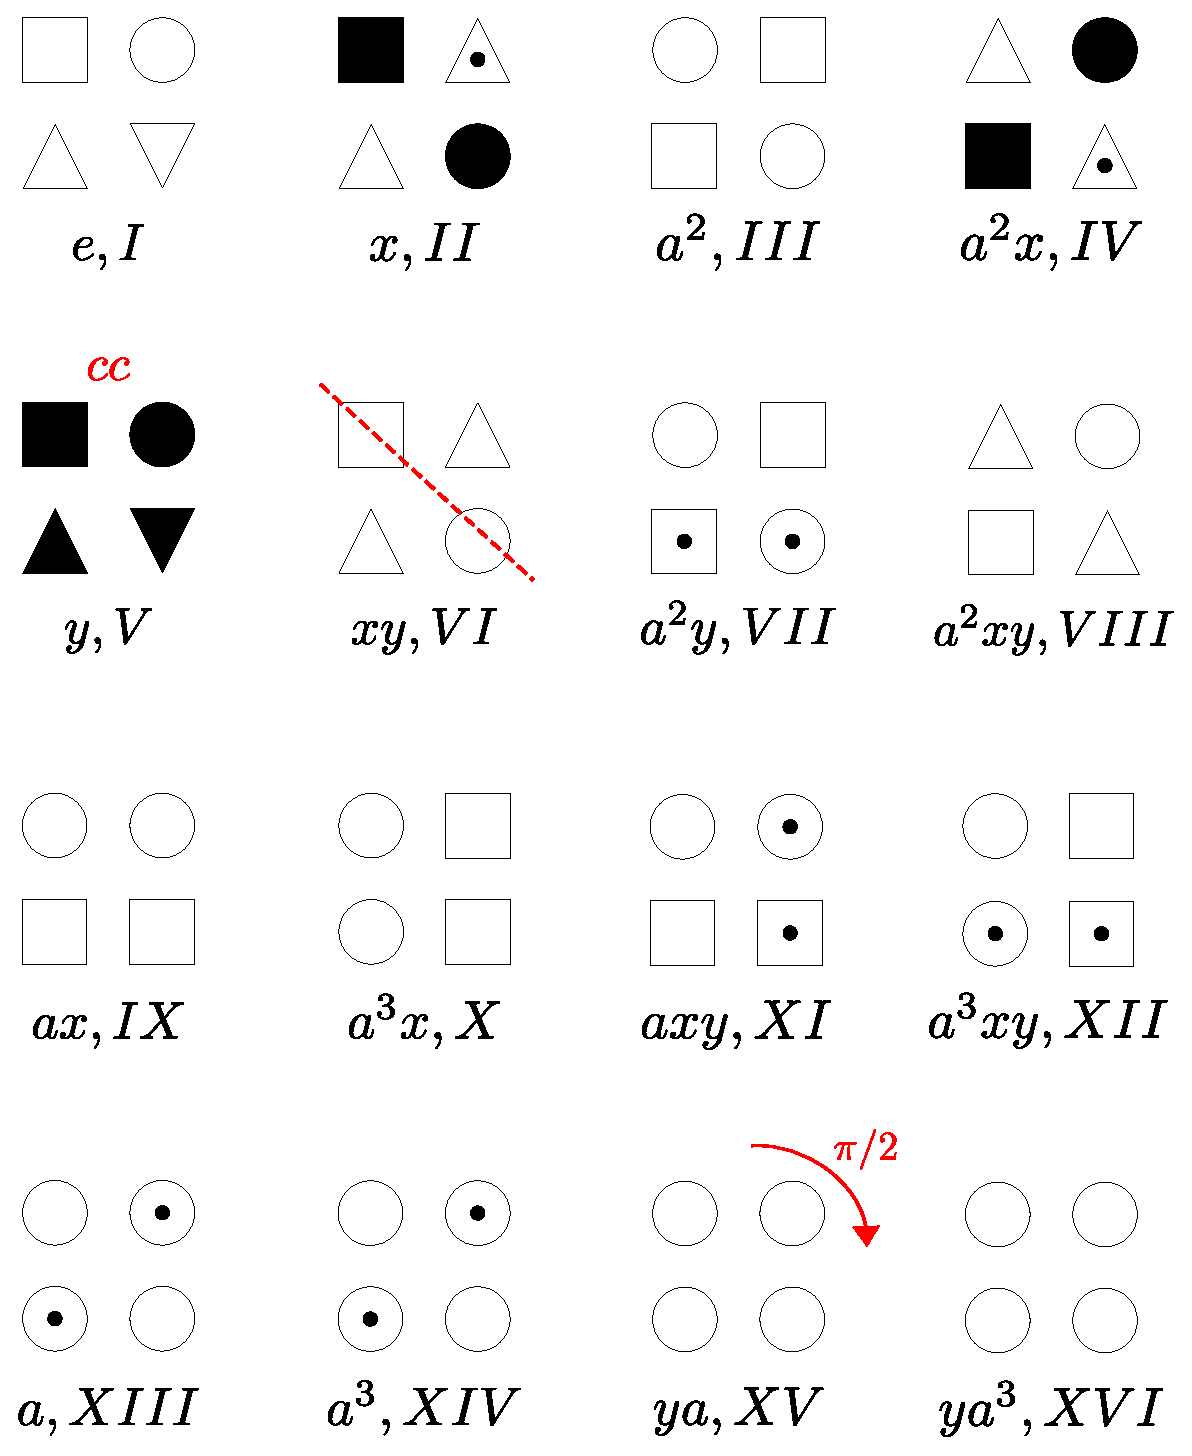
\includegraphics[width=75mm]{Figures/symmetries.eps}
\caption{Representation of $2\times2$ matrices  possesing the  sixteen symmetries compatible with $G_{16}$. The different symbols represent
different complex numbers. The dotted symbols are complex conjugate of undotted ones.  Filled symbols represent real
numbers. The roman number and group-theoretical codes are displayed below each matrix. All symmetry operations
can be constructed from three generators:  among different choices we may use $xy$ (flip along main diagonal), $y$ (complex conjugation), and $ya$ (rotation by $\pi/2$).}
\label{fig16}
\end{center}
\end{figure}
%%%%%%%%%%%%%%%%%


The reader may notice that the symmetries XIII and XIV are special in that they imply the same matrix structure,
as it also happens to
symmetries XV and XVI.
Here the distinction between symmetry operation and symmetry is quite crucial: Whereas
the symmetry operations XIII and XIV (or XV and XVI) are distinct, the corresponding symmetries
imply each other and hold under the same conditions for the matrix elements.  This special relation is explained in detail in the following section.

%\ref{inter}.
%

%%%%%%%%%%%%%%%%%%%%%%%%%%%%%%%%%%%%%%%%%%%%

\section{Implications of one or more  symmetries of the Hamiltonian \label{collapse}}

\subsection{Equivalence of symmetry operations and associated symmetries\label{secx}}
%
The  ``symmetries of $H$'' necessarily form a subgroup $G_{SH}$ with group structure, as the consecutive application of two
superoperators that leave $H$ invariant will also leave $H$ invariant.
This section explores the interplay between $G_{16}$ and $G_{SH}$, specifically the consequences of some existing symmetry. To that end we introduce two concepts: equivalent operations and associated symmetries.
%it is . Specifically An interesting feature of the group $G_{16}$ when realized as the set of operations on a Hamiltonian
%is the set of ``equivalences'' or ``associations'' of the symmetry operations
%which arise as a consequence on an existing symmetry or symmetries of $H$ represented by superoperators that leave $H$ invariant.


%, and we will show the effect of that in the form of equivalences between the other superoperators and associated symmetries.



We will say that,  {\it conditioned to  an existing symmetry or set of symmetries} \{${\cal S}_{i} H=H,
{\cal S}_{j}H=H, ...$\},
{two symmetry operations represented by ${\cal S}_k$  and ${\cal S}_l$ are {\bf equivalent},
${\cal S}_k\sim{\cal S}_l$ (more explicitly,  ${\cal S}_k\sim{\cal S}_l|\{{\cal S}_{i} H=H,
{\cal S}_{j}H=H, ...\}$)
if
${\cal S}_k H={\cal S}_l H$.}



${\cal S}_k\sim{\cal S}_l$  is indeed an equivalence relation in mathematical sense since it is
reflexive (a given superoperator is equivalent to itself); symmetric (if ${\cal S}_k\sim{\cal S}_l$, then
${\cal S}_l\sim{\cal S}_k$); and transitive (if ${\cal S}_k\sim{\cal S}_l$, and
${\cal S}_l\sim{\cal S}_m$, then ${\cal S}_k\sim{\cal S}_m$).



Equivalence relations provide partitions
 of the groups into  equivalence classes. In the $G_{16}$ group, each class is given by the superoperators that are equivalent to each other.   One of these classes is the group $G_{SH}$: All symmetry operations that leave the Hamiltonian invariant are equivalent among themselves and to the identity ${\cal L}_I$.


Equivalent pairs are easily found using the multiplication table of the group.  If ${\cal S}_i H=H$, then ${\cal S}_j={\cal S}_k {\cal S}_i$  (read from the table)
and ${\cal S}_k$  are equivalent.
%We emphasize that the equivalence ${\cal L}_\alpha\sim{\cal L}_\beta$ does not imply that the operations  represent necessarily symmetries of $H$, they may or may not. The equivalence states that the action of these two symmetry operations on $H$ gives the same result, that is all.

An example of equivalence that may be familiar to some
is that, conditioned on $xy H=H$ (which is satisfied in particular by all local potentials if we consider scattering
Hamiltonians in coordinate representation; more generally this symmetry implies that the matrix is complex-symmetric
or, equivalently, self-transpose),
then $a^2y H=a^2x H$. In the alternative operator language this means that, conditioned on $\theta H^\dagger\theta=H$,
we have that $\Pi\theta H\Pi \theta =\Pi H^\dagger \Pi$. In words, with the proper conditioning ($\theta$-pseudohermiticity, i.e., the symmetry of complex-symmetric matrices), the symmetry transformations related to PT-symmetry and to parity-pseudohermiticity give the same result when acting on the Hamiltonian. If it happens that
$H$ is indeed PT-symmetrical (i.e., $\Pi\theta H\Pi \theta=H$), then it will also be parity-pseudo-hermitian
($\Pi H^\dagger \Pi=H$)
and viceversa \cite{Mostafazadeh2010,Znojil2015}. These symmetry pairs  were explored systematically in \cite{Ruschhaupt2017} within the E8 group $\langle x,y,a^2\rangle$ studied  there, conditioned on a given (primary) symmetry. The novelty in the present work is twofold:  we
extend the analysis to $G_{16}$ and also define the equivalence relation more precisely, as a relation among symmetry operations acting on $H$:
as here defined, the equivalent pair is not necessarily a pair of Hamiltonian symmetries, but a pair of operations that, when acting on $H$, give the same result.









Two symmetry operations  represented by ${\cal S}_i$  and ${\cal S}_j$
are {\bf associated symmetry operations} if ${\cal S}_i\in G_{SH}\iff {\cal S}_j\in G_{SH}$.
%{\it and viceversa}.
In our group the two elements of order 4 in a given subgroup Z4 are associated symmetries:  $a$ and $a^3$ are associated, as well as $ay$ and $a^3y$.  The bidirectionality is important. For example $a\in G_{SH}\Rightarrow a^2\in G_{SH}$
but the reverse does not hold, so $a$ and $a^2$  are not associated symmetries.
Two associated symmetries imply the same structure on the Hamiltonian, i.e., the relations
that the matrix elements satisfy are equal in both cases, as illustrated in fig. \ref{fig16}.

Association is a stronger relation than equivalence since it  implies equivalence,
but equivalence does not imply association.

 %

%In prectic, we will specifically study the cases where one or two symmetries are assumed (the higher number of assumed symmetries will give us numerous special cases, but will not be useful to get general rules), and we will also give relevance to the rule generated for the general case (starting with the one symmetry case, to show a gradual development of the theory).

%This section relates closely to the previous one, since the origin of most of the relations  is the group structure of the set of superoperators.
% we will make a reasoning with the effects of this general properties, even so, we will accompany such reasonings with examples.
%Throughout the section it proves convenient to use a notation to label the superoperators which may differ
%from the one in Sec. \ref{sst}.

\subsubsection{Effects of one non-trivial symmetry of the Hamiltonian.}
%
%We will start by giving some simple examples of the more general cases we will study later.
For the following discussion some additional terminology is needed: A ``symmetry or order $n$'' represents the invariance of the Hamiltonian with respect to a superoperator of order $n$ (where $n$ is the minimal power $n\ge 1$ of the superoperator that gives  the identity).


{\it Symmetry of order 2.} Suppose that $H$ is invariant under $x$,  $xH=H$. Since $x^{2}=e$, the group composed by $x$ and $e$ is  in $G_{SH}$ (It might even be the full $G_{SH}$ if there are no other symmetries). Acting with $y$ on $x$ we have that
%and combine it with the members of the 2-group, we get the new superoperator $yx$($=xy$). Since $x$ and $yx$ commute, $yx$ and $y$ will be equivalent,
%
\begin{equation}
yx H=y(xH)=yH,
\end{equation}
%
so $yx\sim y$ conditioned on $xH=H$.
In fact there is nothing special about $y$ here. We can premultiply $x$ by the sixteen members of the group, to get
sixteen superoperators
${\cal S}_j x= {\cal S}_k$. If the index $j$ runs from $1$ to $16$, the index $k$ must jump among  the 16 members of the group
according to the multiplication table ($j\ne k$ except for $j=1$ assigned to the identity). Since $x$ is a symmetry of $H$,  ${\cal S}_k H={\cal S}_j H$, so that ${\cal S}_k\sim {\cal S}_j$ conditioned on $xH=H$.   It might seem that we have sixteen of these
equivalence pairs. However, multiplying ${\cal S}_j x= {\cal S}_k$ by $x$ from the right we find that ${\cal S}_j={\cal S}_k x$. This means that there are in fact only eight equivalence pairs; in other words, the relations (pairs of equivalent operations) are always repeated once.



The only property  of $x$ we have used, apart from representing a symmetry,
is $x^2=1$, so in general
{\it any symmetry of $H$ of order 2, implies eight pairs of equivalent superoperators}.  Conditioned on
$xH=H$,  in particular, we find the equivalences
%
\begin{eqnarray}
x\sim 1, ax\sim a, a^2x\sim a^2, a^3x\sim a^3,
\nonumber\\
ayx\sim ay, a^3yx\sim a^3y, yx^2\sim xy, a^2yx\sim a^2y.
\end{eqnarray}
%


{\it Symmetry of order 4.} Suppose now that $H$ is invariant under $a$ ($aH=H$). By applying $a$ repeatedly  we can create the subgroup of symmetries $\langle a \rangle$  in $G_{SH}$.
%(again it might be the full $G_{SH}$, we do not commit to one or  the other option by now).
Premultiplying the members of the group $\langle a \rangle$ by  $y$, we get the set of superoperators $ya,ya^{2},ya^{3},y$. They are all equivalent,
%
\begin{equation}
yH=y(aH)=yaH=ayH,
\end{equation}
\begin{equation}
yH=y(a^{2}H)=ya^{2}H=a^{2}yH,
\end{equation}
\begin{equation}
yH=y(a^{3}H)=ya^{3}H=a^{3}yH.
\end{equation}
%
The process may be repeated premultiplying the cyclic 4-group by $1$, $x$ and $xy$ instead of $y$. Let us recall that the full group
 of 16 elements may be constructed by multiplying the cyclic group $\langle a\rangle$ by $\langle x,y\rangle$.
Thus, this  premultiplication of $\langle a \rangle$ by the elements of $\langle x,y\rangle=\{1,x,y,xy\}$ gives
all 16 elements of the group $G_{16}$ without repetitions. Each member of $\langle x,y\rangle$ produces an equivalent class of 4 elements, namely,
%
\begin{eqnarray}
1,a,a^2,a^3,
\\
x,xa,xa^2,xa^3,
\\
y,ya,ya^2,ya^3,
\\
xy,xya,xya^2,xya^3.
\end{eqnarray}
%
The first set of 4 elements is formed by symmetries of $H$ while the others need not be symmetries.
Also, multiplication in reverse order, i.e., $\langle a\rangle \times \langle x,y\rangle$ produces exactly the same equivalence classes because of the property $xa=a^3 x$.



If $a^3$ is the assumed  symmetry of $H$
the same structure follows, since $a^3$ generates the same group of symmetries than $a$,
namely $\langle a\rangle=\langle a^3\rangle$.



When the  other elements of order 4, $ay$ and $a^3y$, are symmetries of $H$, they will also imply four sets of equivalent
superoperators,
%
\begin{eqnarray}
1,ay,a^2,ya^3,
\\
x,xay,xa^2,xya^3,
\\
y,y^2a,ya^2,a^3,
\\
xy,xa,xya^2,xa^3,
\end{eqnarray}
%
where, as before, the first set corresponds to symmetries of $H$. The others may or may not  be  symmetries of $H$.

\subsubsection{Consequences of two symmetries.}
%
Now suppose that the distinct superoperators  ${\cal S}_{i}$  and ${\cal S}_{j}$ represent two symmetries of $H$.
The consequences may be deduced by combining the results from the previous subsection.
Let us first recall that the two symmetries may generate groups of 2, 4, and 8 elements corresponding to symmetries as
discussed in the previous section.


- The case corresponding to groups of 2 elements is trivial as it requires that one of the symmetries
is the identity, and the other element should be of order 2.
Therefore the discussion of the consequences has already been done in the previous subsection.


In the following we assume that neither ${\cal S}_{i}$ nor ${\cal S}_{j}$ is the identity.



- A generated group of 4 elements $\langle {\cal S}_{i},{\cal S}_{j}\rangle$ corresponds to commuting operations except the combination of an element of order
4 and an element not in the cyclic groups $Z4$.  All elements of the generated group $\langle {\cal S}_{i},{\cal S}_{j}\rangle$ will be symmetries of $H$.
From there, the group table guarantees that it is always possible to find three other elements ${\cal S}_k$, ${\cal S}_l$, ${\cal S}_m$ such that the products
${\cal S}_{n}\langle {\cal S}_{i},{\cal S}_{j}\rangle$, where $n=k,l,m$, define three classes of equivalent operations. They are equivalent, respectively, to ${\cal S}_k$, ${\cal S}_l$, and ${\cal S}_m$.

Example:  ${\cal S}_{i}=x$;   ${\cal S}_{j}=y$. Then,
%
\begin{equation}
\langle {\cal S}_{i},{\cal S}_{j}\rangle=1,x,y,xy
\end{equation}
%
is a group of symmetries of $H$.
Choosing ${\cal S}_k=a$, ${\cal S}_l=a^2$, ${\cal S}_m=a^3$ we find  the three sets of equivalent operations
%
\begin{eqnarray}
a, ax, ay, axy
\nonumber\\
a^2,a^2x,a^2y,a^2xy
\nonumber\\
a^3,a^3x,a^3y,a^3xy
\end{eqnarray}
%


- Finally, when  $\langle {\cal S}_{i},{\cal S}_{j}\rangle$ has 8 elements, for example $\langle a,y\rangle$,
or $\langle x,a\rangle$, the eight elements are symmetries of $H$,
and {\it all other eight operations are equivalent to each other}. This is easy to prove. Multiplication of
any element ${\cal S}_k$ not in $\langle {\cal S}_{i},{\cal S}_{j}\rangle$ by the eight elements in $\langle {\cal S}_{i},{\cal S}_{j}\rangle$ must produce eight distinct elements not in $\langle {\cal S}_{i},{\cal S}_{j}\rangle$, because in the  group table each
element appears only once in any column (or row). These eight elements  are all equivalent to ${\cal S}_k$.
%If not such an element can be found it means that all elements are symmetries of $H$ and therefore (also) equivalent.
%
%
\subsubsection{Three or more symmetries.}
%
%
With three or more symmetries one may proceed similarly applying and combining the
results of the previous two subsections.
It is advisable to construct first the group generated by
the three superoperators of the symmetries. Several combinations  generate  directly the whole group of 16 elements,
for example $x$, $y$, and any element of order 4.  Other sets of 3 elements generate subgroups of 8 (for example
$\langle x,y,a^2\rangle$), or 4 elements (for example any three elements in a cyclic $Z4$ subgroup).
%
%
\section{Implications of the symmetries on the eigenvalues.\label{sp}}
%
%
If the Hamiltonian obeys a specific symmetry the eigenvectors and eigenvalues will fulfill certain conditions.
For example,  hermitian Hamiltonians imply real eigenvalues, and Hamiltonians that commute with
$\Pi$ will have even or odd eigenvectors.
A full and systematic analysis of the effect of all symmetries on the eigenvectors  is out of the scope of the present work
but we shall discuss here the
effect of the symmetries on the energy spectra because of its physical relevance.
%its completion is left as a pending question for future work. Nevertheless this point is obviously of much physical relevance
%so in this section we advance some important results and discuss several examples.


Let us first recall that the  symmetries for which eigenvalues come in conjugate pairs $E_j,E_j^*$
are symmetries II, IV, V, and VII, equivalently $x$, $a^2x$, $y$, and $a^2y$ in group-theory notation.
%This follows from theorems set by Ali Mostafazadehfazadeh, see e.g. \cite{Simon2019a},
%and corresponds to symmetries that can be expressed either as commutation of $H$ with an antilinear operator,
%or pseudohermiticity of $H$ with respect to some linear operator. T
The reason for having conjugate pairs has been well discussed,
see \cite{Mostafazadeh2002,Mostafazadeh2002a,Mostafazadeh2002b,Simon2019a}, so we shall not insist on it further, except for recalling that
the complex-pair condition implies the possibility to have real eigenvalues. While eigenvalues of Hermitian Hamiltonians $(xH=H)$
are always real, the reality of eigenvalues for symmetries $a^2x$, $y$,
and $a^2y$ is not guaranteed, and
requires specific parameter values, as discussed at length for PT-symmetry $(a^2yH=H)$  since the seminal work
\cite{Bender1998}.

%Some symmetries do not impose any particular relation or conditions  on the eigenvalues.
We shall next pay attention to implications on the eigenvalues of the symmetries of order 4 in the two cycles $Z4$.
% since they do have    implications on the eigenvalues.
For the other symmetries we have found no implications on the possible Hamiltonian eigenvalues, at least when they
are the only symmetries.
%
\subsubsection{$a, a^3$}
%
%
Let as assume that $aH=H$, or, explicitly, that $H=H^\dagger \Pi$.
Now we apply these operators on a right  eigenvector of $H$,
%
\begin{equation}
H|E\rangle=E|E\rangle=H^\dagger |\Pi E\rangle
\end{equation}
%
Acting with $\langle E|$ from the left in the last equality,
%
\begin{equation}
E\langle E|E\rangle=E^*\langle E|\Pi|E\rangle.
\label{condit}
\end{equation}
%
The matrix elements on both sides are real. Now we make use of the fact that
$a^2H=H$, or, translated into operators, $H=\Pi H\Pi$, i.e., $H$ commutes with $\Pi$.
%\Pi|E\rangle=\pm|E\rangle)$.
For right eigenvectors with even or odd parity we find that
%
\begin{eqnarray}
&&{\rm If}\;\; \Pi|E\rangle=|E\rangle \Rightarrow E\, {\rm is\, real},
\\
&&{\rm If}\;\; \Pi|E\rangle=-|E\rangle \Rightarrow E\, {\rm is\, imaginary}.
\end{eqnarray}
%
Of course the same splitting occurs when $a^3H=H$ since $a$ and $a^3$ are associated symmetries.
%
\subsubsection{$ay, a^3y$}
%
We now assume that $ayH=H$, i.e., $\theta H^\dagger\Pi\theta=H$. Note that, as before, $a^2 H=H$
holds as well automatically so that $H$ commutes with $\Pi$.
Making use of the ``diagonal'' biorthogonal  expression $H^\dagger=\sum |\widehat{E}\rangle  E^* \langle E|$
(we omit subindices) one finds, similarly to the previous calculation
%
\begin{equation}
E^*\langle E| \theta |E\rangle=E^*\langle E|\Pi|\theta E\rangle,
\end{equation}
%
which is now solved (assuming $\langle E| \theta |E\rangle\ne 0$)  according to the two possibilities
%
\begin{eqnarray}
&&{\rm If}\;\; \Pi|E\rangle=|E\rangle\Rightarrow   E\, {\rm is\, not\, restricted},
\\
&&{\rm If}\;\; \Pi|E\rangle=-|E\rangle \Rightarrow E=0,
\end{eqnarray}
%
The same result holds for the associated symmetry $a^3yH=H$.
%






\section{Discussion and conclusions\label{cd}}
%
In this work we have explored the symmetry operations on, and symmetries possessed
by, discrete (generally) non Hermitian Hamiltonians.
%\begin{itemize}
We have first seen that symmetry operations for discrete Hamiltonians are richer
that for scattering Hamiltonians because they are not restricted by the properties of the kinetic energy.
A non Abelian group of 16 symmetry operations arises naturally represented by linear and antilinear superoperators
that have geometrical interpretations
in terms of the symmetry operations of the square and complex conjugation.
A symmetry corresponds to the invariance of the Hamiltonian with respect to the transformation implied by one of these superoperators.
We have studied the properties and structure of this group and also
the implications of one or more existing symmetries in the rest of operations of the group,
introducing the  concepts of equivalent operations and of associated symmetries. The implications of some of these symmetries on the energy spectrum have also been discussed.
While some of these symmetries have been extensibly studied,  in particular PT-symmetry ($a^2yH=H$) \cite{Znojil2015}, complex symmetric matrices ($xyH=H$) \cite{Garcia2014},
and of course hermitian matrices ($xH=H)$, the broader frame introduced in this work provides a basis to relate,
understand and exploit multiple symmetries and their interconnections.
Combining discrete and continuous symmetry operations is also possible, as in \cite{Kartashov2014,Zezyulin2017}.






%\end{itemize}

Some open questions and ideas for future work are:
i) To set the relation with optical systems or quantum optical systems and develop
applications such as finding selection rules or device engineering.
In particular physical realizations of non-hermitian symmetries different from $PT$, e.g. with respect to
$a^2$, $xy$, $a^2xy$, are doable
in a quantum optical setting using two-level atoms interacting with a laser beam \cite{Ruschhaupt2004a}.
Our emphasis has been on Hamiltonians but general complex matrices of physical interest, such as  a characteristic matrix of a stratified medium \cite{Born1964},
are of course amenable to be transformed by operations in  $G_{16}$ and may posses some of the
implied symmetries, e.g. with respect to $a$ or $a^3$; ii) To complete a systematic study of the effect of the 16 symmetries on right/left eigenvectors; iii)  To work out a ``representation theory'' for non Hermitian symmetries; iv) To extend the symmetries further. For example the symmetries described have their ``negative'' versions
in the form ${\cal S}H=-H$, or even more generally ${\cal S}H= e^{i\phi} H$, with $\phi$ being a real phase. In this regard it would be very interesting to relate the present work to the Bernard-LeClair symmetry classes
of non-Hermitian random matrices and their variants \cite{Bernard2002, Kawabata2019}. We just note at this point that
some of the symmetries implied by $G_{16}$ are not of the forms considered in $\cite{Bernard2002}$.
    %Discrete Hamiltonian symmetries
%!TEX root = ../Thesis.tex
%Chapter 3

\chapter{Physical Implementation of non-hermitian and non-local hamiltonians}
\label{Chapter3}
\lhead{Chapter 3. \emph{Physical Implementation of non-hermitian and non-local hamiltonians}}
%
Non-Hermitian, one-dimensional  potentials which are also non-local,
allow for scattering asymmetries, namely, asymmetric transmission or reflection responses to the incidence of a particle from left or right.
The  symmetries of the potential
imply selection rules for transmission and reflection. In particular, parity-time (PT)
symmetry or the symmetry  of any local potential do not allow for asymmetric transmission.
We put forward a feasible  quantum-optical implementation
of non-Hermitian, non-local, non-PT potentials to implement different scattering asymmetries, including transmission
asymmetries.
%
\newpage
%
\section{Introduction}
The asymmetric response of diodes, valves, or rectifiers to input direction is of paramount importance in many different fields and technologies, from hydrodynamics  to microelectronics,  as well as in biological systems. We  expect a wealth of applications of such response asymmetries also in the microscopic quantum realm, in particular in  circuits or operations carrying or processing quantum information with moving atoms.
So far  devices such as Maxwell demons, which  let atoms pass one way, have  been instrumental, first as ideal devices to  understand the second law \cite{Maxwell1875,Rex1990}, and also  as practical sorting devices \cite{Ruschhaupt2004,Raizen2005,Dudarev2005,Ruschhaupt2006a,Ruschhaupt2006,Ruschhaupt2006b,Ruschhaupt2007,Raizen2009,Jerkins2010}.

Asymmetric transmission and reflection
probabilities for one-dimensional (1D) particle scattering off  a potential center are not possible if the Hamiltonian is Hermitian \cite{Muga2004,Mostafazadeh2018}.
Non-Hermitian (NH) Hamiltonians representing effective interactions have a long history in nuclear, atomic, and molecular physics, and have become common in optics, where wave equations in waveguides could simulate  Schr\"odinger equations \cite{Ruschhaupt2005,Longhi2017a,Konotop2016}.
%
Non-Hermitian Hamiltonians constructed by analytically continuing Hermitian ones are useful and efficient tools to find resonances \cite{Moiseyev2011}.
They can also be set phenomenologically, e.g. to describe gain and loss
\cite{Ruschhaupt2005},
or be found as effective Hamiltonians for a subspace from a Hermitian Hamiltonian of a larger system
by projection \cite{Feshbach1958,Ruschhaupt2004,Muga2004}.
%

Much of the recent interest in Non-Hermitian Hamiltonians focuses on  parity-time (PT) symmetric Hamiltonians \cite{Bender1998,Znojil2015}  because of their spectral properties and useful applications, mostly in optics  \cite{Longhi2017a,Konotop2016,Longhi2014}, but  alternative symmetries are also being studied \cite{Nixon2016,Nixon2016a,Chen2017,Ruschhaupt2017,Simon2018,Simon2019a,Alana2020,Bernard2002,Kawabata2019}. Symmetry operations
on NH Hamiltonians can be systematized into group structures \cite{Ruschhaupt2017,Simon2019a,Alana2020}.  In particular for
1D particle scattering off a potential center, the different Hamiltonian symmetries imply
selection rules for asymmetric transmission and reflection \cite{Ruschhaupt2017,Simon2019a}.\footnote{Throughout the paper we assume a linear theory for systems whose wave equation is linear in the wavefunction.}
Whereas hermiticity does not allow for any asymmetry in transmission and reflection probabilities,   PT symmetry or
the symmetry of local potentials, technically ``pseudohermiticy with respect to time reversal'' \cite{Ruschhaupt2017},
do not allow for  asymmetric transmission \cite{Muga2004,Mostafazadeh2018}, see symmetries II (Hermiticity), VII (PT symmetry),  and VI
(time-reversal pseudohermiticity) in table \ref{condi}.
(Here a ``local potential'' is defined as one whose only non-zero elements in coordinate representation are diagonal, whereas a non-local one has  non-zero nondiagonal elements.)
%
%
Thus  non-local, non-PT, and non-Hermitian potentials are needed to implement a rich set of scattering
asymmetries, and in particular asymmetric transmission.

In this paper we put forward a physical realization of  effective NH, non-local  Hamiltonians which do not posses PT symmetry.
Non-local potentials for asymmetric scattering had been constructed as mathematical models \cite{Ruschhaupt2017}, but a physical implementation  had been so far elusive.
Using Feshbach's projection technique it is found that the
effective potentials for a ground-state atom crossing a laser beam in a region of space are generically non-local and non-Hermitian. Shaping the spatial-dependence of the, generally complex, Rabi frequency, and selecting a specific laser detuning allows us to produce different potential symmetries and asymmetric scattering effects, including asymmetric transmission.

After a lightning review of Hamiltonian symmetries and the corresponding scattering selection rules in Sec. \ref{ssh},
we shall  explain in Sec. \ref{enl} how to generate different NH symmetries in a quantum optical setting of an atom impinging on a laser illuminated region. Finally we provide specific example devices (constructed using numerical optimisation) with different asymmetric scattering responses in Sec. \ref{exa}. Realistic experimental parameters are also examined. The asymmetric behavior can be intuitively understood based on a classical approximation of the motion and the non-commutativity of rotations on the Bloch sphere, which gives good estimates for the potential parameters, see Sec. \ref{class}.

%
%
%
\section{Symmetries of Scattering Hamiltonians\label{ssh}}
%
%
We consider one-dimensional  scattering Hamiltonians  $H=H_0+V$, where $H_{0}$
is the kinetic energy for a particle of mass $m$,
and
$V$ is the  potential, which is assumed to decay fast enough on both sides so that $H$ has a continuous spectrum and scattering eigenfunctions. These eigenfunctions may be chosen so that asymptotically, i.e., far from the potential center,  they are superpositions of an incident plane wave and a reflected plane wave on one side, and a transmitted plane wave on the other side. Reflected and transmitted waves include corresponding amplitudes, whose squared-modulii
(scattering coefficients hereafter) sum to one for Hermitian potentials. Instead, NH potentials
may produce  absorption or gain.


There are eight different symmetries that $H$ could fulfill, see table \ref{condi},
with the forms
%
\begin{eqnarray}
	AH&=&HA,
	\\
	AH&=&H^{\dagger}A,
	\label{pseudohermiticityPhysicalImplementation}
\end{eqnarray}
%
%
where $A$ is a unitary or antiunitary operator in the Klein four-group \linebreak $K_{4}=\lbrace 1,\Pi,\theta,\Pi\theta \rbrace$ \cite{Ruschhaupt2017}.
Relation \eqref{pseudohermiticityPhysicalImplementation} is called here $A$-pseudohermiticity of $H$ \cite{Mostafazadeh2010,Ruschhaupt2017}.
The operators $1$, $\Pi$, $\theta$ and $\Pi\theta$ are the identity, parity, time reversal,
and the consecutive (commuting) application of both operators.
Acting on position eigenvectors $|x\rangle$,
$\Pi c|x\rangle =c|-x\rangle$, and $\theta c |x\rangle = c^* |x\rangle$, for any  complex number $c$. Note that symmetry I is a trivial symmetry and is satisfied for all Hamiltonians.

%
The eight symmetries  may be regarded as the invariance of the Hamiltonian with respect to
eight symmetry operations that form the Abelian group E8 \cite{Simon2019a}. They are all operations that can be done by inversion, transposition, complex conjugation, and their combinations.
Making use of generalized unitarity relations and  the relations implied by the symmetries on $S$-matrix elements,
the transmission and reflection amplitudes for right and left incidence, $T^r$, $R^r$ and $T^l$, $R^l$, can be  related
to each other,
as well as their modulii \cite{Ruschhaupt2017}.  ``Right and left  incidence'' are here shorthands for ``incidence {\it from} the right'',
and ``incidence { from} the left'', respectively.

The possible asymmetric responses are allowed or forbidden, according to selection rules,  by the symmetries of the Hamiltonian.
If we impose that the transmission and reflection coefficients  have only 0 or 1 values,  a convenient reference scenario for  devices intended to manage quantum-information applications, six possible scattering asymmetries may be identified \cite{Ruschhaupt2017}, see table \ref{table2PhysicalImplementation}. It is useful to label them according to the response  to incidence from the left/right. The possible responses are encoded in the  letters ${\cal{A}}$,
for ``absorption'', and ${\cal{T}}$ and ${\cal{R}}$ for ``transmission'' and ``reflection'', separated by ``$/$''. The
letters on the left of $/$ are for left incidence, and the ones on the right are for right incidence. For example ${\cal T/A}$ means transmission for left incidence and absorption for right
incidence. From the selection rules \cite{Ruschhaupt2017}, it is possible to determine which symmetries allow for a given device, see table \ref{table2PhysicalImplementation}.

The relations between the symmetries and ``reciprocity'' are surely worth spelling out, in view of many works and discussions in optics \cite{Lin2011,Feng2011,Fan2012,Peng2014}. ``Reciprocity'' is a somewhat vague term with different meanings for different authors and communities, the reviews \cite{Potton2004} and \cite{Deak2012} give  some useful  background. A primary formulation regards reciprocity as the property of detecting the  same effects when interchanging source and detector without changing the scatterer. This  concept has lead to  different formalizations that fix in more detail what is exactly meant by ``same effects'' and ``interchanging source and detector''.
In 1D scattering problems we may first  distinguish  a reciprocity for scattering amplitudes or for scattering coefficients (their modulus squared). We shall hereafter focus on  coefficients as in the rest of  the paper.
Another distinction can be made between reflection and transmission reciprocities, namely, a system with $|R^l|^2=|R^r|^2$
would be ``reflection reciprocal'' and if $|T^l|^2=|T^r|^2$ the system would be transmission reciprocal.\footnote{Incidentally, for reflection reciprocity, ``interchanging source and detector'' has to be understood in momentum space rather than spatially.}
A formal definition of reciprocity is that, for some antiunitary operator $K$ \cite{Deak2012},
%
\begin{equation}
	\label{reci}
	HK=KH^\dagger.
\end{equation}
%
It follows that the scattering transition  matrix obeys in momentum representation \cite{Deak2012}
%
\begin{equation}\label{tt}
	\la p|{\sf T}|p'\ra=\la Kp'|{\sf T}|Kp\ra.
\end{equation}
%
In our symmetry classification, symmetries VI and VIII obey by definition reciprocity conditions of the form \eqref{reci}.
Inserting the results in the exact forms of transmission and reflection amplitudes, which depend on diagonal and non-diagonal elements of the transition matrix, respectively,   see e.g.  \cite{Muga2004},
different physical consequences follow:  In symmetry VI, $K=\Theta$, $|Kp\ra=|-p\ra$, and the reciprocity condition implies transmission reciprocity.
In symmetry VIII, $K=\Pi\Theta$ and $|K p\ra=|p\ra$, so the reciprocity condition implies reflection reciprocity.
A first relevant observation is this: an arbitrary reciprocity condition of the form \eqref{reci}, does not necessarily imply symmetrical transmission. A second point is that ``scattering selection rules'',  i.e., the set of forbidden phenomena, or compulsory relations among right and left coefficients, see table 1 in \cite{Ruschhaupt2017}, depend as well on generalized unitary relations. Putting together the effect of symmetries on transition or
$S$-matrix elements and generalized unitarity relations, it turns out that
symmetries II (Hermiticity) and III (parity) are not capable of any,  reflection or transmission, asymmetry; symmetries VI (time reversal pseudohermiticity) and VII (PT symmetry) allow for reflection asymmetry
but not for transmission asymmetry;  symmetries V (time-reversal symmetry) and VIII (PT pseudohermiticity) allow for
transmission asymmetry but not for reflection asymmetry, whereas I (trivial symmetry) and IV (parity pseudohermiticity) allow for both scattering asymmetries.
Note also the importance on non-locality for asymmetric transmission: All local potentials do satisfy automatically symmetry VI, and are therefore necessarily transmission reciprocal. Let us insist once more than all these results are for linear (Schr\"odinger) dynamics.
Nonlinearity allows to break down these selection rules \cite{Lin2011,Peng2014,Xu2014}.




%---------------------------------------------------------------------------------------------
\begin{table}[t]

	\caption{Conditions leading to  specific symmetries in the potential \eqref{effpot}. A given symmetry also implies others, see the last column.\label{condi}}
	\hspace*{-0.1cm}
	\scalebox{.94}{
	\begin{tabular}{lcc}
		\hline\hline
		Symmetry& Conditions & Implies
		\\
		\hline
		(I)\;$1H=H1$ &   none & -
		\\
		(II)\;$1H=H^\dagger 1$ &  $q=-q^{*}$ (i.e. $\operatorname{Re}q=0$) & I
		\\
		(III)\;$ \Pi H=H\Pi$ &  $\Omega(x)=e^{i\phi}\Omega(-x)$ & I
		\\
		(IV) $\Pi H=H^\dagger \Pi$ &  $q=-q^{*}$ \& $\Omega(x)=e^{i\phi}\Omega(-x)$ & III,\! II,\! I
		\\
		(V) $\Theta H=H\Theta$ &  $q=-q^{*}$ \& $\Omega(x)=e^{i\phi}\Omega(x)^*$ & {\small VI,\! II,\! I}
		\\
		(VI) $\Theta H=H^\dagger\Theta$ &  $\Omega(x)=e^{i\phi}\Omega(x)^*$ & I
		\\
		(VII) $\Theta\Pi H=H\Theta \Pi$ &  $q=-q^{*}$ \& $\Omega(x)=e^{i\phi}\Omega(-x)^*$ & VIII,\! II,\! I
		\\
		(VIII)\,$\Theta\Pi H=H^\dagger \Theta \Pi$ &  $\Omega(x)=e^{i\phi}\Omega(-x)^*$  & I
		\\
		\hline\hline
	\end{tabular}
	}
\end{table}
%---------------------------------------------------------------------------------------------

%%%%%%%%%
\begin{table}[t]
	\caption{Device types for  transmission and/or reflection asymmetry in the first row (see main text for nomenclature,
	binary values ($0$ or $1$) for the transmission and reflection coefficients are considered here as an ideal case).
	The second row gives the corresponding symmetries  that allow
	each device.
	\label{devices}}
	\vspace*{.0cm}
	\label{table2PhysicalImplementation}
	\centering
	\scalebox{0.90}{
	\begin{tabular}{cccccc}
		$\cal{TR/A}$ & $\cal{T/R}$ & $\cal{T/A}$ & $\cal{TR/R}$ & $\cal{R/A}$ & $\cal{TR/T}$ \\
		I            & I           & I,VIII      & I,VIII       & I,VI        & I, IV, VI, VII
	\end{tabular}}
\end{table}

%
%
%
%
%

%
\section{Effective non-local potential for the ground state of a two-level atom\label{enl}}
%
The key task is now to physically realize some of the potential and device types described in the previous section. We start with a two-level atom with ground level $|1\ra$ and excited state $|2\ra$ impinging onto a laser illuminated region. For a full account of the model and further references see
\cite{Ruschhaupt2009}. The motion is assumed one dimensional, either because the atom is confined in a waveguide or because the direction $x$ is uncoupled to
the others.
We only account explicitly for atoms before the first spontaneous emission in the wavefunction
\cite{Hegerfeldt1996,Damborenea2002,Navarro2003}.
If the excited atom emits a spontaneous photon it disappears from the coherent wavefunction ensemble.
We assume that no resetting into the ground state occurs. The physical mechanism
may be an irreversible decay into a third level  \cite{Oberthaler1996}, or atom ejection from the waveguide or the privileged 1D direction due to  random recoil  \cite{Streed2006}.
The state ${\bf\Phi}_k=\left(\begin{smallmatrix}\phi_k^{(1)}\\\phi_k^{(2)}\end{smallmatrix}\right)$
for the atom before the first spontaneous emission impinging with wavenumber $k$
in a laser adapted  interaction picture,
obeys, after applying the rotating wave approximation,  an effective stationary Schr\"odinger equation
with a time-independent Hamiltonian \cite{Ruschhaupt2004a,Ruschhaupt2009}
%
${\cal H}{\bf\Phi}_k(x)=E{\bf\Phi}_k(x)$,
%
where
%
\begin{eqnarray}
	{\cal H}&=& H_0{\bf 1}+ {\cal V}=\frac{1}{2m}\left(
	{{p}^2\atop 0}{0\atop {p}^2}\right)+ {\cal V}(x),
	\\
	{\cal V}(x) &=&
	\frac{\hbar}{2}\left(
	{0\atop \Omega(x)^*}\;\;\;\;
	{\Omega(x)\atop -(2\Delta+i\gamma)}
	\right).
\end{eqnarray}
%
We assume perpendicular incidence of the atom on the laser sheet for simplicity, oblique incidence is treated e.g. in  \cite{Ruschhaupt2007,Ruschhaupt2009}.
Here $E=\hbar^2 k^2/2m$ is the energy, and
$\Omega(x)$ is the position-dependent, on-resonance Rabi frequency, where real and imaginary parts may be controlled independently
using two  laser field quadratures  \cite{Zhang2013};
$\gamma$ is the inverse of the life time of the excited state;
$\Delta=\omega_{L}-\omega_{12}$
is the detuning (laser angular frequency minus the atomic transition
angular frequency $\omega_{12}$);
${p}=-i\hbar\partial/\partial x$ is the momentum operator;
and ${\bf 1}=|1\ra\la 1|+|2\ra\la 2|$ is the unit operator
for the internal-state space.
Complementary projectors
%
$P=|1\ra\la 1|$ and $Q=|2\ra\la 2|$
%
are defined to select ground and excited state components.
Using the partitioning
technique \cite{Feshbach1958,Feshbach1962,Levine1969},
we find for the ground
state amplitude $\phi_k^{(1)}$ the equation
%
\begin{equation}\label{effecti}
	E\phi_k^{(1)}(x) = H_0\phi_k^{(1)}(x)+\!
	\int\! dy\, \la x,1|{\cal W}(E)|y,1\ra \phi_k^{(1)}(y),
\end{equation}
%
where
%
$
{\cal W}(E)=P{\cal V}P+P{\cal V}Q(E+i0-Q{\cal H}Q)^{-1}Q{\cal V}P,
$
%
is generically non local and energy dependent. Specifically, we have now achieved
a physical realization of an effective (in general) non-local, non-Hermitian potential whose kernel has the form
%
\begin{eqnarray}
	\hspace*{-.3cm}V (x,y) = \la x,1|{\cal W}(E)|y,1\ra = \frac{m}{4} \frac{e^{i|x-y|q}}{i q}
	\Omega(x)\Omega(y)^*,
	\label{effpot}
\end{eqnarray}
%
%
where
$
q=\frac{\sqrt{2mE}}{\hbar}(1+\mu)^{1/2},\;\;
{\rm Im}\,q\ge 0,
\label{qeq}
$ and
$
\mu=\frac{2\Delta+i\gamma}{2E/\hbar}.
$
%
Eq. \eqref{effpot} is worked out  in momentum representation to do the integral
using the residue theorem.
This is a generalized, non-local version of the effective potentials known for the ground state
\cite{Chudesnikov1991,Oberthaler1996}, which are found from Eq. \eqref{effpot}  in the large $\mu$ limit \cite{Ruschhaupt2004a}.
The reflection and transmission amplitudes $R^{r,l}$ and  $T^{r,l}$ may be calculated directly
using  the potential  \eqref{effpot} or as  corresponding amplitudes for
transitions from ground state to ground state in the full two-level theory see Appendix \ref{Appendix:NumericalCalculationOfTandR}.


%
\subsection{Possible symmetries of the non-local potential}
%
The necessary conditions for the different symmetries of the potential \eqref{effpot} are outlined in the second column of  table \ref{condi}. For example,
symmetry III (parity) requires that $V(x,y)=V(-x,-y)$ \cite{Ruschhaupt2017}. Inserting the functional form of the potential from Eq. \eqref{effpot} into this condition, it results in the requirement $\Omega(x) \Omega(y)^* = \Omega(-x) \Omega(-y)^*$. This is fulfilled if $\Omega(x)=\Omega(-x)e^{i \phi}$ with some arbitrary phase freedom $\phi$.

Since $\Omega(x)$ does not depend on $q$, symmetries IV, V and VII imply that symmetry II is obeyed as well (Hermiticity).
Moreover symmetry III (parity) should be discarded for our purpose since it does not allow for asymmetric transmission or reflection
\cite{Ruschhaupt2017}.
This leaves us with three interesting symmetries to explore:
VI, which allows for  asymmetric reflection; VIII which allows for asymmetric transmission, and  I,
which in principle allows for arbitrary asymmetric responses, except for physical limitations imposed by
the two-level model see Appendix \ref{Appendix:NumericalCalculationOfTandR}.


%
%
As seen from  table \ref{condi}, $\operatorname{Re}(q)=0$ makes the potential Hermitian so we shall avoid this condition.
If $\gamma=0$,   $\mu \in \mathbb{R}$. Hence $\mu+1<0$ gives $\operatorname{Re}(q)=0$ and $\mu+1>0$ gives
$\operatorname{Im}(q)=0$. $\mu+1>0$ amounts to a condition on the detuning compared to the incident energy, namely $\Delta>-E/\hbar$.
In the following examples we implement potentials with symmetries VIII, VI, and I, with detunings and energies satisfying the condition $\mu+1>0$.
%
%
%

%
%
%
\section{Design of asymmetric devices\label{exa}}
%
%
We will now apply this method to physically realize non-local potentials of the form \eqref{effpot}.
%
We  shall work out  explicitly a ${\cal T/A}$ device with symmetry  VIII, a ${\cal R/A}$ device with symmetry  VI, and a ``partial''-${\cal TR/A}$ device,  having 1/2 transmission and reflection coefficients from the left, with symmetry I. The  ${\cal T/A}$ and the ``partial''-${\cal TR/A}$ device have transmission asymmetry so they cannot be built with local or $PT$-symmetric  potentials.
%, whereas   to design asymmetric devices which can be shown not to be implementable with a one-dimensional, one-channel, local potential.
Let us  motivate the effort with some possible applications, relations  and analogies of these devices.
${\cal T/A}$ and ${\cal R/A}$ are, respectively, transmission and reflection filters. They are analogous to
half-wave electrical rectifiers that either let the signal from one side ``pass'' (transmitted) or change its sign (reflected)
while suppressing the other half signal.  They may play the role of half-rectifiers in atomtronic circuits.
A ${\cal T/A}$ device allows us, for example, to empty a region of selected particles, letting them go away while not letting particles in.
The ``atom diode'' devices worked out e.g. in \cite{Ruschhaupt2004,Ruschhaupt2006a,Ruschhaupt2006,Ruschhaupt2007}
where of type ${\cal R/A}$. As the mechanism behind them was adiabatic, a broad range of momenta with the desired asymmetry
could be achieved. In comparison the current approach is not necessarily adiabatic so it can be adapted to faster processes.

As for the ``partial''-${\cal RT/A}$ device,  it reflects and transmits from one side while absorbing from the
other side. In an optical analogy an observer from the left perceives it as a darkish mirror.
An observer from the right ``sees'' the other side because of the allowed transmission
but cannot be seen from the left since  nothing is transmitted from right to left. Our device is necessarily ``partial'' one as
there cannot be  net probability gain because of the underlying two-level system, and a ``full'' version with both reflection and transmission coefficients equal to one
would need net gain.

The three devices are worked out for $\gamma=0$, a valid approximation for  hyperfine transitions. %, although this is by no means a necessary assumption.
We assume  for the Rabi frequencies the forms
%
\begin{eqnarray}
	\Omega_{\rm VIII} (x) &=& a [g(x+x_0) + i  g(x-x_0)],
	\nonumber\\
	\Omega_{\rm VI} (x) &=&  b g(x+x_0) + c g(x-x_0),
	\nonumber\\
	\Omega_{\rm I} (x) &=&  - i b g(x+x_0) + c g(x-x_0),
	\label{3omegas}
\end{eqnarray}
%
in terms of smooth, realizable Gaussians $g(x) =  \exp[-{x^2}/{w^2}]$.
We fix $2 d$ as an effective finite width
of the potential area beyond which the potential is negligible and assumed to vanish. We will express in the following the different length parameters as a multiple of $d$ to keep results general.
In addition, we will use as a scaling factor for the velocity $v_{d} = {\hbar}/({m d})$, and for time $\tau={m d^2}/{\hbar}$.

In the following calculations we fix the width of the Gaussians to be $w= {\sqrt{2}}d/{10}$.
We always first set a target velocity $v_0$ to achieve the desired asymmetric scattering response.
The real parameters $a$, $b$, $c$, $x_0$ in Eq. \eqref{3omegas}, and  $\Delta$
are then numerically optimized with the GRAPE (Gradient Ascent Pulse Engineering) algorithm \cite{Khaneja2005,Wu2015}.

The Rabi frequencies will fulfill the indicated symmetries VIII, VI, and I. $\Omega_{\rm VI}(x)$ should not be even (i.e. $b \neq c$) to avoid symmetry II. In addition, $\Omega_{\rm I}(x)$ should not fulfill any other symmetry than ${\rm I}$.
The corresponding Rabi frequencies $\Omega(x)$ are  depicted in Figs. \ref{fig_t_a}, top row.
The scattering coefficients are shown in the bottom row. Fig. \ref{fig_t_a} demonstrates that the three potentials satisfy the asymmetric response conditions imposed
at the selected velocity and also in a region nearby.

The ``partial''-${\cal TR/A}$  device fullfills $\absq{T^l} = \absq{R^l} = 1/2$ and full absorption from the right.
The potential we use for that device has symmetry I only, i.e., ``no symmetry'' other than the trivial commutation with the identity. No other potential symmetry would allow this type of device.

The effective non-local potential $V(x,y)$, see Eq. \eqref{effpot}, corresponding to the $v/v_d$ ratios used for the three devices is shown in Fig. \ref{fig_poten1}. Note that the non-local potential has dimensions  energy/length, so  we
divide the absolute value by a factor $V_0=\hbar^2/(m d^3)$ to plot a dimensionless quantity.


% -------------------------------------------------------------
\begin{figure*}
	\begin{center}
		\includegraphics[width=0.28\linewidth]{Figures/asym_fig_t_a_400_pot.pdf}
		\includegraphics[width=0.28\linewidth]{Figures/asym_fig_r_a_400_pot.pdf}
		\includegraphics[width=0.28\linewidth]{Figures/asym_fig_1_2_tr_a_8_pot.pdf}\\
		\includegraphics[width=0.29\linewidth]{Figures/asym_fig_t_a_400.pdf}
		\includegraphics[width=0.29\linewidth]{Figures/asym_fig_r_a_400.pdf}
		\includegraphics[width=0.29\linewidth]{Figures/asym_fig_1_2_tr_a_8.pdf}
	\end{center}
	\caption{Left column: ${\cal T/A}$ device with symmetry VIII.
	Top: $\Omega_{\rm VIII}(x)$;
	Bottom:  transmission and reflection coefficients. $v_0/v_d=400$, $a\tau = 2618.19$,
	$x_0/d = 0.1532$, $\tau\Delta = 1413.01$.
	%
	Middle column: ${\cal R/A}$ device with symmetry VI.
	Top: $\Omega_{\rm VI} (x)$ (it is real); Bottom:  transmission and reflection coefficients. $v_0/v_d=400$,
	$b \tau =  -244516.1$,
	$c\tau = 167853.9$,
	$x_0/d = 0.1679$,
	$\tau\Delta= 193.508$.
	%
	Right column: ``Partial''-${\cal TR/A}$ device with symmetry I.
	Top:  $\Omega_{\rm I}(x)$, real (blue, solid line) and imaginary parts (orange, dashed line);
	Bottom: transmission and reflection coefficients. $v_0/v_d=8$, $b\tau =  102.6520$,
	$c \tau =  165.8355$,
	$x_0/d = 0.1648$,
	$\tau\Delta= 90.5337$. In all cases $\tau={m d^2}/{\hbar}$ and $v_{d} = {\hbar}/({m d})$.
	\label{fig_t_a}}
\end{figure*}
% -------------------------------------------------------------

%--------------------------------------------------------------------------
\begin{figure*}
	\begin{center}
		\includegraphics[width=0.28\linewidth]{Figures/asym_fig_t_a_400_eff_pot_abs.pdf}
		\includegraphics[width=0.28\linewidth]{Figures/asym_fig_r_a_400_eff_pot_abs.pdf}
		\includegraphics[width=0.28\linewidth]{Figures/asym_fig_1_2_tr_a_8_eff_pot_abs.pdf}\\
		\includegraphics[width=0.29\linewidth]{Figures/asym_fig_t_a_400_eff_pot_arg.pdf}
		\includegraphics[width=0.29\linewidth]{Figures/asym_fig_r_a_400_eff_pot_arg.pdf}
		\includegraphics[width=0.29\linewidth]{Figures/asym_fig_1_2_tr_a_8_eff_pot_arg.pdf}
	\end{center}
	\caption{Nonlocal potentials  $V(x,y)$: absolute value (top), argument (bottom).
	Left column: Potential for ${\cal T/A}$ device with symmetry VIII.
	Middle column: Potential for ${\cal R/A}$ device with symmetry VI.
	Right column: ``Partial''-${\cal TR/A}$ device with symmetry I.
	$V_0=\hbar^2/(md^3)$.}
	\label{fig_poten1}
\end{figure*}
%--------------------------------------------------------------------------

In the parameter optimization we see that increasing the velocities further does not pose a problem for the ${\cal T/A}$
device, it is more challenging for a ${\cal R/A}$ device, and it is quite difficult for the partial-${\cal RT/A}$ device.  The device ${\cal T/A}$ is feasible for an experimental implementation  as the ratio $v_0/v_d$ can be easily increased to desired values, for  reasonable values of the
Rabi frequency and laser waist \cite{Zeyen2016}.

Moreover the velocity width with the desired behavior is much broader for ${\cal T/A}$. Therefore a ${\cal T/A}$
device is the best candidate for
an experimental implementation.
As a check of feasibility, let us assume a Beryllium ion. Its hyperfine structure provides a good  two-level system
for which we can neglect decay (i.e. $\gamma\approx 0$ is indeed realistic). We have $m=1.49\times 10^{-26}$ kg
and set a length $d=10\, \mu$m compatible with the small laser waists (in this case 1.4 $\mu$m) achieved for individual ion
addressing \cite{Zeyen2016}. The scaling factors take the values
%
\begin{eqnarray}
	v_d&=&0.67\, {\rm mm/s},
	\nonumber\\
	\tau&=&1.49\times 10^{-2}\, {\rm s},
	\nonumber
\end{eqnarray}
%
which gives  $v\approx$ 27 cm/s for $v/v_d=400$, (again, we see no major obstacle to get devices for higher velocities,
in particular the classical approximations in Sec. \ref{class} can be used to  estimate the values of the parameters)
and Rabi frequencies, see Fig. \ref{fig_t_a},  in the hundreds of kHz range. The relative ion-laser beam velocity could be as well
implemented  by moving the beam in the laboratory frame.

%
%
\section{Classical approximation for ${\cal T/A}$ device \label{class}}
%
%
In a ${\cal T/A}$ device such as the one presented an incident plane wave from the left ends up as a pure transmitted wave with no reflection or absorption.
However, a wave incident from the right is fully absorbed. How can that be? Should not the velocity-reversed motion
of the transmitted wave lead to the reversed incident wave?
%Obviously that is not the case, and a formal answer to that question  is that $V$ is not time-reversal invariant.
For a more intuitive understanding we may seek help in the underlying two-level model.
In the larger space the potential is again local and Hermitian. A simple semiclassical
approximation is to assume that the particle moves with  constant speeds $\pm v$ for left ($v>0$) or right ($-v<0$) incidence,  so that at a given time it is subjected to  the $2\times2$ time-dependent potentials
${\cal V}(\pm vt)$. The incidence from the left and right give different time dependences for the potential. The scattering problem then reduces to solving the time-dependent Schr\"odinger equation for the amplitudes of a two-level atom with time-dependent potential, i.e. to solving the following time-dependent Schr\"odinger equation ($\gamma = 0$)
%
\begin{eqnarray}
	i \hbar \frac{\partial}{\partial t} \chi_\pm(t)
	= {\cal V} (\pm v t) \chi_\pm(t),
\end{eqnarray}
%
with the appropriate boundary conditions $\chi_+ (-\infty) = \chi_- (-\infty) =\left(\begin{smallmatrix} 1\\ 0\end{smallmatrix}\right)$. The  solutions for $v/v_d = 400$
%9.1
are shown in Fig. \ref{fig_t_a_approx}.
In Fig. \ref{fig_t_a_approx}(a), $\chi_+ (t)$ (left incidence) is depicted:  the particle ends  with high probability in the ground state at final time. In Fig. \ref{fig_t_a_approx}(b), $\chi_- (t)$ (right incidence) demonstrates  the ground state population is transferred to the excited state. Projected onto the ground-state level alone,
this corresponds to full absorption of the ground state population at final time.

For an  even rougher but also illustrative picture,  again in a semiclassical time-dependent framework, we  may substitute the smooth Gaussians for Re$(\Omega)$ and Im$(\Omega)$ in Fig. \ref{fig_t_a} by two simple, contiguous square functions of height
$\Omega>0$ and width $\tilde{w} > 0$. Then, the $2\times2$ potential at a given time is, in terms of Pauli matrices,
%
\begin{eqnarray}
	{\cal V} (x) = \frac{\hbar}{2}\Delta (\sigma_Z-{\mathbf 1})+ \frac{\hbar}{2} \left\{\begin{array}{cc}
	\Omega\sigma_X & -\tilde w < x < 0\\
	-\Omega\sigma_Y & 0 < x < \tilde w\\
	0 & \mbox{otherwise}
	\end{array}\right.
\end{eqnarray}
%
where $x = \pm v t$ and let ${\sf T}=2 \tilde w/v$.

% ------------------------------------------------------------------------------
\begin{figure}
	\begin{center}
		\includegraphics[width=0.48\linewidth]{Figures/asym_fig_t_a_approx_left.pdf}
		\includegraphics[width=0.48\linewidth]{Figures/asym_fig_t_a_approx_right.pdf}
	\end{center}
	\caption{Simplified model of the asymmetric ${\cal T/A}$ device with symmetry VIII: (a) $\chi_+(t)$, (b) $\chi_-(t)$; ground-state population $\absq{\chi_{\pm(t),1}}$ (blue, solid line), excited-
	$\absq{\chi_{\pm(t),2}}$ (orange, dashed line). $v/v_d = 400$, $a\tau = 2618.19$,
	$x_0/d = 0.1532$, $\tau\Delta = 1413.01$.
	\label{fig_t_a_approx}}
\end{figure}
% ------------------------------------------------------------------------------

% ------------------------------------------------------------------------------
\begin{figure}
	\fbox{
	\begin{minipage}{8cm}
		\flushleft  (a) Order of rotations:  first  $R_1({\sf T}/2)$ (left figure) and then $R_2({\sf T}/2)$ (right figure)
		\begin{center}
			\vspace*{-0.32cm}
			\includegraphics[width=0.49\linewidth]{Figures/"asym_fig_sphere_left1"}\,\includegraphics[width=0.49\linewidth]{Figures/"asym_fig_sphere_left2"}\\[0.1cm]
		\end{center}
		(b) Order of rotations: first $R_2({\sf T}/2)$ (left figure) and then $R_1({\sf T}/2)$ (right figure).
		\vspace*{-0.32cm}
		\begin{center}
			\includegraphics[width=0.49\linewidth]{Figures/"asym_fig_sphere_right1"}\,\includegraphics[width=0.49\linewidth]{Figures/"asym_fig_sphere_right2"}
		\end{center}
		\vspace*{-.8cm}
	\end{minipage}
	}
	\caption{Simplified time-dependent model of the asymmetric ${\cal T/A}$ device with symmetry VIII: Bloch sphere explaining non time-reversal invariance, see text for details. The state trajectories are depicted in two-steps on the sphere. The rotation axes are
	also depicted. (a) The process simulates incidence from the left. The state starts and ends in $|1\ra$. (b) The process simulates incidence from the right. The state starts at $|1\ra$ and ends at $|2\ra$.
	\label{fig_t_a_simple2}}
\end{figure}
% ------------------------------------------------------------------------------


The time-evolution of this process, $\chi_\pm (t)$,
up to a phase factor may be regarded as
two consecutive rotations $R_j=e^{-i{\beta}{\bf n}_j\cdot {\boldsymbol{\sigma}}/2}$ ($j=1,2$), with $\beta=\frac{{\sf T}}{2}\sqrt{\Omega^2+\Delta^2}$, of the two-level state on the Bloch sphere about the axes
%
\begin{eqnarray}
	{\bf n}_1&=&\frac{1}{\sqrt{\Omega^2+\Delta^2}}(\Omega,0,\Delta), %real
	\\
	{\bf n}_2&=&\frac{1}{\sqrt{\Omega^2+\Delta^2}}(0,-\Omega,\Delta). %imag
\end{eqnarray}
%
The initial state at time $t=-{\sf T}/2$ is again $\chi_+ (-{\sf T}/2) = \chi_- (-{\sf T}/2) =\left(\begin{smallmatrix} 1\\ 0\end{smallmatrix}\right)$.
The unitary time-evolution operator to reach the final time ${\sf T}/2$ takes the form
$e^{i\Delta {\sf T}/2}R_2 R_1$ for  incidence from the left ($\chi_+$) and
$e^{i\Delta {\sf T}/2}R_1 R_2$ for incidence from the right ($\chi_-$).
The time ${\sf T}$ and the parameters $\Omega, \Delta$ will be fixed to reproduce the results of the full calculation with the exact model, namely,
so that the system starts in the ground state to end either in the ground state
($\absq{\chi_{+} ({\sf T}/2)} = 1$)
or in the excited state by performing the rotations in one order or the reverse order
($\absq{\chi_{-} ({\sf T}/2)} = 0$). This gives $\Omega/\Delta = \sqrt{2}$ and ${\sf T}= 4\pi/(3 \sqrt{3} \Delta)$. It follows that ${\bf n}_1=\frac{1}{\sqrt{3}}(\sqrt{2},0,1)$ and ${\bf n}_2=\frac{1}{\sqrt{3}}(0,-\sqrt{2},1)$.

The different outcomes can thus be understood as the result of the \linebreak non-commutativity of rotations on the Bloch sphere, see
Fig. \ref{fig_t_a_simple2}: In Fig. \ref{fig_t_a_simple2}(a), first the rotation $R_1({\sf T}/2)$ and then the rotation $R_2({\sf T}/2)$ are performed. Starting in the ground state $\ket{1}$, the system ends up  in the excited state $\ket{2}$.
In Fig. \ref{fig_t_a_simple2}(b),  first the rotation $R_2({\sf T}/2)$ and then the rotation $R_1({\sf T}/2)$ are performed:  now the system starts and ends  in the ground state $\ket{1}$.

These results can be even used to approximate the parameters of the potential in the quantum setting.
As an approximation of the height $a$ we assume that the area $a \int_{-\infty}^\infty dx \, g(x) = a \sqrt{\pi} w$
is equal to $\tilde w \Omega = {{\sf T}} v_0 \Omega/2 =
v_0 \pi ({2}/{3})^{3/2}$. This results in an
approximation $a \approx \frac{v_0}{w} \sqrt{\pi}\, ({2}/{3})^{3/2}$. As an additional approximation, we
assume that $(a/\sqrt{2})/\Delta \approx {\Omega}/{\Delta} = \sqrt{2}$, so we get
$\Delta \approx a/2 \approx \frac{v_0}{2 w} \sqrt{\pi}\, ({2}/{3})^{3/2}$. A comparison between
these approximations and the numerically achieved parameters, see Fig. \ref{fig_t_a_param}, shows a good agreement
over a large velocity range. This allows one to find good initial values for further numerical optimization.

% ------------------------------------------------------------------------------
\begin{figure}
	\begin{center}
		\includegraphics[width=0.48\linewidth]{Figures/asym_fig_t_a_param1.pdf}
		\includegraphics[width=0.48\linewidth]{Figures/asym_fig_t_a_param2.pdf}
	\end{center}
	\caption{Asymmetric ${\cal T/A}$ device with symmetry VIII: comparison between numerically achieved parameters (red dots) and approximated parameters (blue, solid lines) versus velocity $v_0$.
	(a) Height of Rabi frequency $a$, (b) detuning $\Delta$.
	\label{fig_t_a_param}}
\end{figure}
% ------------------------------------------------------------------------------

%
%
%
%

%
%
\section{Discussion}
Non-Hermitian Hamiltonians display many interesting phenomena which are
impossible for a  Hermitian Hamiltonian  acting on the same Hilbert space. In particular, in the Hilbert space of
a single, structureless particle on a line formed by square integrable normalizable functions, Hermitian Hamiltonians do not allow, within a linear theory, for asymmetric scattering transmission and reflection coefficients.
% for right/left incidence of a particle off a potential center.
However,
non-Hermitian Hamiltonians do.   Since devices of technological interest, such as one-way filters for transmission or reflection, one-way barriers, one-way mirrors, and others, may be built based on such scattering response asymmetries, there is both fundamental
interest and applications in sight to implement Non-Hermitian scattering Hamiltonians.    This paper is a step forward in that direction, specifically we propose a quantum-optical implementation of potentials with asymmetric scattering response.
They are non-local and non-PT symmetrical, which allows for asymmetric transmission.

In general the chosen Hilbert space may  be regarded as a subspace of a larger space. For example,  the space of a ``structureless particle'' in 1D is the ground-state subspace
for a particle with internal structure, consisting of two-levels in the simplest scenario.
It is then possible to regard the Non-Hermitian physics in the reduced space
as a projection of the larger space, which may itself be driven by a  Hermitian or a Non-Hermitian Hamiltonian.
We have seen the Hermitian option in our examples, where we assumed a zero decay constant, $\gamma=0$, for the excited state.
A non-zero $\gamma$ implies  a Non-Hermitian  Hamiltonian in the larger two-level space. The description may still be
enlarged,  including  quantized field modes to account for the atom-field interaction with a Hermitian Hamiltonian.
As an outlook, depending on the application, there might be the need for a more fundamental and detailed descriptive level. Presently we discuss the desired physics (i.e., the scattering asymmetries) at the level of the smallest 1D space of the ground state, while taking refuge in the
two-level space to find a feasible physical implementation.
    % Physical Implementation of non-hermitian and non-local hamiltonians


% ------------ PART II: Heat Rectification ---------------------------------------------------------
\part{Heat rectification in mesoscopic systems}
%!TEX root = ../Thesis.tex
%IntroductionPartII

\chapter*{Introduction to Part II}
\addcontentsline{toc}{chapter}{Introduction to Part II}
\label{IntroductionPartII}
\lhead{Introduction to Part II} % Write in your own chapter title to set the page header

Radiation, heat and electricity are prominent mechanisms of energy transport. In particular, the two last mechanisms have a dominant role in technology. Modern information processing rests on electronic devices like the diode and the transistor. However, there is not an existing analogous technology to the diodes and transistors based on control of heat currents driven by phonons, \textit{i.e.} the quasiparticles describing vibrational modes. An explanation to this phenomenom could be that phonons are more difficult to control than electrons since, as oposed to electrons, they don't have mass or electrical charge.

Energy transport due to phonons has a rich diversity of physical mechanisms worth exploring to design phononic devices. Together with advancements in nanotechnology, this could boost the growth of phononics. The thermal rectifier, or thermal diode would be a primary building block to develop phononic devices and that is why I decided to study it.

Thermal rectification is the physical phenomenon, analogous to electrical current rectification in diodes, in which heat current through a device or medium (the thermal diode or rectifier) is not symmetric with respect to the exchange of the bath temperatures at the boundaries. It was  first observed in 1936 by Starr in a junction between copper and cuprous oxide \cite{Starr1936}. The theoretical work started much later  using as rectifiers simple anharmonic chain models
with different segments \cite{Terraneo2002,Li2004}. These papers sparked much research that continues to this day. Research on thermal rectification has gained a lot of attention in recent years as a key ingredient to build prospective devices to control heat flows similarly to electrical currents \cite{Roberts2011,Li2012}. There are  proposals to engineer thermal logic circuits \cite{Ye2017} in which information, stored in thermal memories \cite{Wang2008}, would be processed in thermal gates \cite{Wang2007}. Such thermal gates, as their electronic counterparts,  will require thermal diodes and thermal transistors  to operate \cite{Li2006,Joulain2016}.
Heat rectifying devices would also be quite useful in nano electronic circuits, letting delicate components dissipate heat while being protected from external heat sources \cite{Roberts2011}.

Most work on thermal diodes has been theoretical with only a few experiments
like \cite{Chang2006,Kobayashi2009,Leitner2013,Elzouka2017}.
A relevant attempt to build a thermal rectifier was based on a graded structure made of carbon and boron nitride nanotubes that transports heat between a pair of heating/sensing circuits \cite{Chang2006}. One of the ends of the nanotube is loaded with a deposition of another material, which makes the heat flow better from the loaded end to the unloaded end. However, rectifications were small, with rectification factors (relative
heat-flow differentials) around $7\%$.

Much of the theoretical effort in thermal rectification research has been aimed at improving the rectification factors and the features of the rectifiers. The first approach to designing thermal diodes consisted in using chains of oscillators segmented into two or more regions with different properties \cite{Terraneo2002,Li2004,Li2008,Hu2006}, which is reminiscent of the idea of the $p-n$ junction in electric diodes. It was soon realized, however, that the performance of segmented rectifiers was very sensitive to the size of the device, i.e., rectification decreases with increasing the length of the rectifier \cite{Hu2006}. To overcome this limitation two ideas were proposed. The first one consists in using graded rather than segmented chains, i.e., chains where some physical property varies continuously along the site position such as the mass of particles in the chain \cite{Wang2012,Chen2015,Romero-Bastida2017,Yang2007,Romero-Bastida2013,Dettori2016,Pereira2010,Pereira2011,Avila2013}. The second one uses chains with long-range interactions (LRI), such that all the sites in the lattice interact with each other \cite{Chen2015,Bagchi2017,Pereira2013}. The rationale behind was that in a graded system new asymmetric, rectifying channels are created, while the long-range interactions create
also new transport channels, avoiding the usual decay of heat flow with size \cite{Chen2015}. Besides a stronger rectification power, LRI graded chains are expected to have better heat conductivity than segmented ones. This is an important point for technological applications, because devices with high rectification factors are not useful if the currents that flow through them are very small.

Another main focus of the theoretical research in thermal rectification is the search for the fundamental factors that contribute to the emergence of rectification. Historically the crucial elements for having rectification were identified as the presence of some structural asymmetry in the system and of nonlinear (anharmonic) forces \cite{Zeng2008,Katz2016,Li2008,Hu2006,Benenti2016,Li2012,Segal2005,Segal2005b}, which lead to a temperature dependence of the phonon bands or power spectral densities. A match or mismatch of the phonon bands of neighboring parts of the chain implies corresponding good or bad conduction so the
sign of the temperature bias may affect the conduction and lead to rectification when the spectra of the parts are affected differently by the bias reversal. However more recent research in the topic pointed out  that anharmonicity is not a necessary condition for an asymmetric match/mismatch and therefore for rectification \cite{Pereira2017}. Rectification also occurs in simple (minimalistic) harmonic models that incorporate some structural asymmetry and temperature-dependence of the model parameters \cite{Pereira2017}. This dependence may indeed result from an underlying, more intricate  anharmonic system by linearization of the stochastic dynamics \cite{Pereira2017,Pereira2019}, or it may have a different origin \cite{Simon2019}.

In the chapters of this section I will present the contributions I made together with my group and other collaborators to the field of thermal rectification in chains of oscillators. In Chapter \ref{Chapter4} I present a model of a thermal rectifier that relies on a localized impurity in the middle of the chain. With this approach we make a proposal that diverges from the prevalent approach of using segmented chains. In Chapter \ref{Chapter5} we make a proposal for a thermal rectifer in a chain of trapped ions with a graded frequency distribution. This prototype seizes the combined power of long range interactions, which are naturally present in trapped ion chains due to the Coulomb force, and graded structures. This proposal brings the added value of being possible to be experimentally realized, since trapped ions are a solid technology in quantum technologies. Finally, in Chapter \ref{Chapter6} I study heat transport in a solvable model of two connected oscillators to explore the origin of thermal rectification. It is believed that non-linear interactions are needed in order to have rectification, since a system with non-linear interactions will have a temperature-dependent spectra. I show, however that it is possible to have temperature dependent features in a linear system that lead to rectification, in agreement with other works like \cite{Pereira2017}.

%!TEX root = ../Thesis.tex
%Chapter 4

\chapter{Local Rectification of Heat Flux}
\label{Chapter4}
\lhead{Chapter 4. \emph{Local Rectification of Heat Flux}} % Write in your own chapter title to set the page header
%
In this chapter, a model for an atom-chain thermal rectifier is presented. The atoms in the chain are trapped in on-site harmonic potentials, and interact with their nearest neighbours by Morse potentials (or also by harmonic potentials in a simplified version). The chain is homogeneous except for a local modification of the interactions and trapping potential at one site, the ``impurity''. The rectification mechanism is due here to the localized impurity, the only asymmetrical element of the structure, apart from the externally imposed temperature bias, and does not rely on putting in contact different materials or other known mechanisms such as grading or long-range interactions.  The effect survives if all interaction forces are linear except the ones for the impurity.

The rest of the chapter is organized as follows. In section \ref{sec:homogeneous_chain}, I shall describe the homogeneous 1D chain, without the impurity.  For this system, I numerically solve the dynamical equations, to show that the usual heat conduction applies. In section \ref{sec:Impurity_rectifier}, I modify the potentials for one of the atoms and demonstrate the rectification effect. I also observe rectification when all the interaction Morse potentials are substituted by harmonic oscillators. Finally, in section \ref{sec:chapter4_Discussion}, I summarize and discuss the results of this chapter.

\section{Homogeneous one-dimensional chain\label{sec:homogeneous_chain}}

I start with a homogeneous 1D chain with $N$ atoms coupled at both extremes to heat baths, at different temperatures $T_h$ and $T_c$ for ``hot" and ``cold" respectively. The baths are modeled with a Nos\' e-Hoover method as described in \cite{Martyna1992}. Atoms $1$ and $N$ represent the first and the $N$-th atom in the chain, from left to right, that will be in contact with the baths. All the atoms are subjected to on-site potentials and to nearest-neighbor interactions, and their equilibrium positions $y_{i0}$ are assumed to be equally spaced by a distance $a$.
$x_i= y_i-y_{i0}$,
$i=1,...,N$, represent the displacements from the equilibrium positions of the corresponding atoms
with positions $y_i$.

%%%%%%%%%%%%%%%%%%%%%%%
\begin{figure}
\centering
\includegraphics[width=0.65\linewidth]{Figures/FIG1.pdf}
\caption{(a) On-site potentials: harmonic potential centered at the equilibrium position of each atom (dashed blue line) as a function of the displacement from this position $x_i=y_i-y_{i0}$ in $a-$units, and the on-site potential for the impurity, $i=N/2+1$
($N$ even, red solid line). (b) Interaction potentials as a function of the distance between nearest neighbors: Morse potential
(blue dashed line) valid for all atoms except for $i=N/2+1$, $N$ even, where the modified potential (red solid line) is used.
The harmonic approximation of the Morse potential is also depicted (eq. (\ref{Vhar}), black dots, only used for fig. \ref{fig:chapter4_figure5}, below).
Parameters: $D=0.5$, $g=1$, $\gamma = 45$, $d=100$ and $b=105$, used throughout the chapter.
}
\label{fig:chapter4_figure1}
\end{figure}
%%%%%%%%%%%%%%%%%%%%%%%%%

The classical Hamiltonian of the atom chain can be written in a general form as
%
\begin{equation}
\label{GH}
%GH=general Hamiltonian
H=\sum_{i=1}^{N} H_i,
\end{equation}
%
with
%
\begin{eqnarray}
\label{GH2}
%GH=general Hamiltonian
H_1&=&{{p^2_1} \over {2m}} +U_1(x_1)+V_L,
\nonumber\\
H_i&=&{{p^2_i} \over {2m}} +U_i(x_i)+V_i(x_{i-1},x_i)  \quad i=2,...,N-1,
 \nonumber\\
H_N&=&{{p^2_N} \over {2m}} +U_N(x_N)+V_N(x_{N-1},x_N) + V_R,
\end{eqnarray}
%
where the $p_i$ are the momenta, $U_i(x_i)$ is the on-site potential for the $i$th atom, and $V_i(x_{i-1},x_i)$ represents the atom-atom interaction potential. $V_R$ and $V_L$ are the interactions coupling the boundary atoms to the Nos\'e-Hoover thermostats, see \cite{Martyna1992}.

%%%%%%%%%%%%%%%%%%%%%%%%%%%%
\begin{figure}
\centering
\includegraphics[width=0.65\linewidth]{Figures/FIG2.pdf}
\caption{Symmetric temperature profiles for a homogeneous chain, without impurity.  For $T_{h}=T_{L}$, $T_c=T_R$ (red solid dots) the (absolute value of) the heat flux is $J_{L\rightarrow R}$, equal to $J_{R\rightarrow L}$ for the reverse configuration of the bath temperatures, $T_{h}=T_{R}$, $T_c=T_L$
(black empty squares). Parameters as in fig. \ref{fig:chapter4_figure1}.}
\label{fig:chapter4_figure2}
\end{figure}
%%%%%%%%%%%%%%%%%%%%%%%%%%%%%%

There are a large number of 1D models that obey this general Hamiltonian. Different choices of the trapping and interaction potentials would give different conductivity behaviors. I choose a simple form of the Hamiltonian in which each atom is subjected to a harmonic on-site potential and a Morse interaction potential between nearest neighbors (see fig. \ref{fig:chapter4_figure1}, dashed lines),
%
\begin{eqnarray}
\label{HO}
%HO=Harmonic oscillator
U_i(x_i)&=&{1 \over 2} m \omega^2 x^2_i,
%\end{equation}
%\begin{equation}
\\
\label{IH}
%IP=Interaction potential
V_i(x_{i-1},x_i)&=&D\left \{e^{-\alpha [x_i-x_{i-1}]}-1\right \}^2,
\end{eqnarray}
%
where $\omega$ is the trapping angular frequency, and $D$ and $\alpha$ are time-independent parameters of the Morse potential.
A ``minimalist version'' of the model where $V$ becomes the harmonic limit of eq. (\ref{IH}), dotted line in fig. 1,
 will also be considered in the final discussion,
%
\begin{equation}
\label{Vhar}
{V}_i(x_{i-1},x_i)=k(x_i-x_{i-1})^2/2,\;k=2D\alpha^2.
\end{equation}
%
For convenience, dimensionless units are used and the mass of all particles is set to unity.

I start by studying the homogeneous configuration with no impurity and potentials (\ref{HO}) and (\ref{IH}), solving numerically the dynamical equations for  the Hamiltonian (\ref{GH}) with a Runge-Kutta-Fehlberg algorithm. I have chosen a low number of atoms, $N=20$,  with thermal baths at $T_h=0.20$ and $T_c=0.15$ at both ends of the chain with 16 thermostats each. The real temperature is related to the dimensionless one through $T_{real}=T m a^2 \omega^2/k_B$ so, for typical values  $m\approx10^{-26}$ kg, $\omega \approx 10^{13}$ s$^{-1}$, $a\approx 10^{-10}$ m, and using $k_B =1.38 \times 10^{-23}$ JK$^{-1}$,
the dimensionless temperatures $0.15,\, 0.20$, translate into $100,\, 150$ K. It is advisable to use temperatures around these values in order to ensure that the displacements of the particles are realistic \cite{Casati1984}.

%%%%%%%%%%%%%%%%%%%%%%%%%%%%%%%%%%
\begin{figure}
\centering
\includegraphics[width=0.65\linewidth]{Figures/FIG3.pdf}
\caption{Temperature profile along the homogeneous chain for different number of atoms: 100 (dotted black line), 125 (dashed blue line) and 150 (solid red line). The atom sites have been rescaled with the total number of atoms.
%, showing the convergence of the spatial profile of the local temperature $T_i$.
The time averages have been carried over a time interval of $\approx 2 \times 10^6$ after a transient of $\approx 1\times 10^5$. In the inset (a), the product $JN$ vs. $N$ demonstrates that for long chains $JN$ is independent of $N$. In (b) the linear dependence of $J$ with $\Delta T$ for a fixed number of atoms, $N=100$, is shown. Parameters as in fig. \ref{fig:chapter4_figure1}.}
\label{fig:chapter4_figure3}
\end{figure}
%%%%%%%%%%%%%%%%%%%%%%%%%%%%%%%%%%%%%%%%

First I demonstrate the conductivity behavior of the model.
%that our system satisfies Fourier's heat law for the heat flux, $J=\kappa \nabla T$.
%, so it shows normal thermal conductivity. ESTE CONCEPTO TIENE QUE VER CON EL TAMA�O?
To this end, I calculate the local heat flux $J_i$ and temperature $T_i$, performing the numerical integration
%of eq. (\ref{GH2})
for long enough times to reach the stationary state.
The local temperature is found as the time average $T_i= \langle p_i^2 / m \rangle$, whereas
%After a transient, the local temperature is given by the time average $T_i=\langle p_i^2\rangle$.
$J_i$,  from the continuity equation
%, $\dot H(x,t)+divJ(x,t)=0,$
\cite{Hu1998}, is given by
%
%Fourier law: temperature gradient vanishes with N
\begin{equation}
\label{heatflux}
J_i=-\dot x_i {{\partial V(x_{i-1},x_{i})} \over {\partial x_i}}.
\end{equation}
%
From now on I only consider the time average $\langle J_i (t)\rangle$, which converges to a constant value for all sites once the system is in the stationary nonequilibrium state. I depict the temperature profiles, for $N=20$, first with $T_L=T_h$ and $T_R=T_c$
($L$ and $R$ stand for left and right) and after switching the positions of the thermal baths in fig. \ref{fig:chapter4_figure2}. The profiles are symmetric, as expected, and the heat flux does not have a preferred direction  \cite{Hu1998,Terraneo2002}. Denoting the absolute values of the fluxes from the left (when $T_L=T_h$) as
$J_{L\rightarrow R}$, and from the right (when $T_R=T_h$) as
$J_{R\rightarrow L}$, I find that $J_{L\rightarrow R}=J_{R\rightarrow L}=J=1.6\times 10^{-2}$, in the dimensionless units, consistent with the values found in other models \cite{Terraneo2002,Hu1998}.

%%%%%%%%%%%%%%%%%%%%%%%%%%%%%%%%%%%
\begin{figure}
\centering
\includegraphics[width=0.65\linewidth]{Figures/FIG4b.pdf}
\caption{Temperature profile for the chain of $N=20$ atoms, with an impurity in the $N/2+1$ position, with $T_L=T_h$ and $T_R=T_c$ (circles) and with the thermostat baths switched (squares).
Parameters as in fig. \ref{fig:chapter4_figure1}.
(a) $T_c=0.15$, $T_h=0.2$. $J_{L\rightarrow R}=0.00769$ vs $J_{R\rightarrow L}=0.00581$, with gives a rectification $R=31 \% $; (b) $T_c=0.025$, $T_h=0.325$. $J_{L\rightarrow R}=0.0499$ vs  $J_{R\rightarrow L}=0.0140$, with $R=256 \%$.}
\label{fig:chapter4_figure4}
\end{figure}
%%%%%%%%%%%%%%%%%%%%%%%%%%%%%%%%%%%%%%%%%

The profile of the temperature is linear with boundary non-linearities at the edges, close to the thermal baths,  due to the boundary conditions \cite{Lepri1997}. In fig. \ref{fig:chapter4_figure3}, I depict $T_i$ vs $i/N$ for $N=100, 125$ and $150$ with the same boundary conditions. For these
larger atom numbers  I have connected the first 3 and the last 3 atoms to the Nos\'e-Hoover baths.
%The temperature gradient scales as $N^{-1}$, which is also true for many other different models \cite{Hu1998}.
In the inset (a) of fig. \ref{fig:chapter4_figure3}  the product $JN$ vs. $N$ is plotted, showing that for a low $N$ limit there is a well defined conductivity per unit length whereas for longer chains, $JN$ tends to be constant  which indicates a normal thermal conductivity independent of the length. Fixing the number of atoms to 100, as in the inset (b) of fig. \ref{fig:chapter4_figure3},  I observe a linear dependence between the flux and $\Delta T$.
%Fourier law, $J=\kappa \nabla T$, is fulfilled.

\section{Impurity-based thermal rectifier \label{sec:Impurity_rectifier}}

To rectify the heat flux I modify the potentials for site $j=N/2+1$ with $N$ even, as
%
%\begin{equation}
%\label{IMP1}
%IMP1=impurity in absolute position
%U_j(y_j,t)=d e^{-b [y_j(t)-y_{d}]} +ge^{-\gamma [y_j(t)-y_{j-1}(t)-\epsilon]}
%\end{equation}
%with $y_{d}=y_{d,0}-a/3$.  Written in terms of the displacements, $x_j$,
%
\begin{eqnarray}
\label{IMP}
%IMP=impurity
U_j(x_j,t)&=&d e^{-b [x_j(t)+a/3]},
\\
V_j(x_{j-1},x_j,t)&=&ge^{-\gamma [x_j(t)-x_{j-1}(t)+a/2]}.
\end{eqnarray}
%
All the parameters involved, $d, b$, and $g,\gamma$ are time-independent. In fig. \ref{fig:chapter4_figure1} the modifications introduced with respect to the ordinary sites are shown (solid lines).  The different on-site and interaction terms introduce soft-wall potentials
(instead of hard-walls to aid in integrating the dynamical equations) that make it difficult for the impurity to transmit its excitation to the left whereas left-to-right transmission is still possible.
This effect is facilitated by the relative size of the coefficients, $a/3<a/2$, that determine the position of the walls.
% that I fixed after some experimentation.
These positions imply that an impurity excited by a hot right bath cannot affect its left cold neighbour near its equilibrium position at the $j-1$ site.
However, if the left $j-1$ atom is excited from a hot bath on the left,
it can get close enough to the impurity to kick it and transfer kinetic energy.

\begin{figure}
\centering
\includegraphics[width=0.65\linewidth]{Figures/FIG5new.pdf}
\caption{Rectification factor $R$ as a function of the temperature difference between ends of the chain of atoms, $\Delta T$.
%The rectification factor shows a very strong dependency on $\Delta T$.
I have changed both $T_h$ and $T_c$ according to $T_c=0.15-(\Delta T-0.05)/2$ and $T_h=0.2+(\Delta T-0.05)/2$, with $N=20$,  keeping the rest of parameters as in fig. \ref{fig:chapter4_figure1}.
Interatomic potentials: Morse potential, eq. (\ref{IH}) (black line with circles, see the temperature profiles of extreme points in fig. \ref{fig:chapter4_figure4}); harmonic potential, eq. (\ref{Vhar}) (red line with squares).}
\label{fig:chapter4_figure5}
\end{figure}

After extensive numerical simulations, I have chosen the values of these parameters as in fig. \ref{fig:chapter4_figure1}, such that the conductivity in the forward direction, $J_{L\rightarrow R}$, and the rectification factor, defined as $R=(J_{L\rightarrow R}-J_{R\rightarrow L}) / J_{R\rightarrow L}\times 100$,
are both large for $T_h=0.2$, $T_c=0.15$. A large $R$ without a large $J_{L\rightarrow R}$ could in fact be useless \cite{Roberts2011}.
%($R=0$ would represent a perfectly symmetric heat conduction.).
Note that the parameters are not necessarily the optimal combination, which in any case would depend on the exact definition of ``optimal'' (technically on how $J_{L\rightarrow R}/J$ and $R$ are weighted and combined in a cost function and on the limits imposed on the
parameter values). This definition is an interesting question but it goes beyond the scope of this chapter, which is to demonstrate and discuss the effect of the localized impurity.

I have used again $N=20$ atoms connected to baths of 16 thermostats each, with the same temperatures as for the homogeneous chain, and numerically solved the dynamical equations
to calculate the local temperature and the heat flux for both configurations of the baths. The interatomic potential for the regular atoms is the Morse potential (\ref{IH}).
In fig. \ref{fig:chapter4_figure4}(a), the temperature profiles show a clear asymmetry between ${L\rightarrow R}$ and ${R\rightarrow L}$. Specifically, I find $J_{L\rightarrow R}=7.6 \times 10^{-3}$ and $J_{R\rightarrow L}=5.8 \times 10^{-3}$ which gives
$R=31\%$. The effect decays with longer chains,  with, for example, $R=19\%$ for $N=100$, and R=17.8\% for $N=150$.

\begin{figure}
\centering
\includegraphics[width=0.65\linewidth]{Figures/FIG6.pdf}
\caption{Temperature profile for a harmonic interacting chain of $N=20$ atoms, with an impurity in the $N/2+1$ position, with $T_L=T_h$ and $T_R=T_c$ (circles) and with the thermostat baths switched (squares), for (a) $\Delta T = 0.05$ and (b)  $\Delta T = 0.3$. The corresponding rectification factors are (a) $R=18\%$ and (b) $R=85\%$. Parameters regarding the impurity are the same as in fig. \ref{fig:chapter4_figure1}.
}
\label{fig:chapter4_figure6}
\end{figure}

These temperature profiles depend on the difference between the bath temperatures, see e.g. fig. \ref{fig:chapter4_figure4}(b). Increasing the temperature gap, but  keeping $T_h$ low enough so that the displacement of the atoms from their equilibrium positions is realistic, I find higher values of $R$. Figure \ref {fig:chapter4_figure5} shows the strong dependence of $R$ with $\Delta T$ (black circles). I have changed both $T_h$ and $T_c$ so that the mean temperature $(T_c+T_h)/2$ remains constant.

\section{Discussion\label{sec:chapter4_Discussion}}

I have presented  a scheme for thermal rectification using a one-dimensional chain of atoms which is homogeneous except
for the special interactions of one of them, the impurity, and the couplings with the baths at the boundaries. These proof-of-principle results for an impurity-based rectification mechanism may encourage further exploration of the impurity-based rectification, in particular of the effect of different forms for the impurity on-site potential and its interactions with neighboring atoms.
In contrast to the majority of chain models, the structural asymmetry in the present model is only in the impurity. The idea of a localized effect was already implicit in early works on a two-segment Frenkel-Kontorova
model \cite{Li2004,Hu2006}, where rectification depended crucially on the interaction constant coupling between the two segments.
However, the coupling interaction was symmetrical and the asymmetry was provided by the different nature
(parameters) of the segments put in contact.
Also different from common chain models are the potentials chosen here. Instead of using the Morse potential as an on-site model, see e.g.  \cite{Terraneo2002},
I have considered a natural setting where this potential characterizes the interatomic interactions,
and the on-site potential is symmetrical with respect to the equilibrium position, and actually harmonic.
The numerical results indicate that this model is consistent with normal conduction,
and also helps to isolate and identify the local-impurity mechanism for rectification.
In this regard it is useful to consider a further simplification, in the spirit of the minimalists models
proposed by Pereira \cite{Pereira2017}, so as to distill further the essence of the local rectification mechanism.
If the Morse interatomic interaction is substituted by the corresponding harmonic interaction, see the black dotted line in fig. \ref{fig:chapter4_figure1}(b), the rectification effect remains, albeit slightly reduced, see fig. \ref{fig:chapter4_figure5}. The chain is then perfectly linear with the only non-linear exception  localized
at the impurity.
The temperature dependent feature mentioned in \cite{Pereira2017} as the second necessary condition for rectification besides asymmetry, is here localized in the impurity too, and consists of a different
capability to transfer kinetic energy depending on the temperatures on both sides of the impurity.
Figure \ref{fig:chapter4_figure6} shows temperature profiles for the purely harmonic chain to be compared with the Morse-interaction
chain in fig. \ref{fig:chapter4_figure4}. Flatter profiles are found on both sides of the impurity, as corresponds to the abnormal transport expected for harmonic chains \cite{Lepri2003}. It would be interesting to combine the impurity effect with other rectification mechanisms (such as grading, long-range interactions, or use of different segments), or with more impurities in series to enhance further the rectification effect.

Even though the motivation was to mimic the effect of a localized atom diode that lets atoms pass only one way,
unlike the atom diode \cite{Ruschhaupt2004}, all interactions in the present model
are elastic. The model may be extended by adding an irreversible,  dissipative element so as to induce not only rectification but a truly Maxwell demon for heat transfer \cite{Skordos1992,Ruschhaupt2006}.
On the experimental side, one dimensional chains of neutral atoms in optical lattices can be implemented with cold atoms \cite{Bloch2005}.
An impurity with different internal structure could be subjected to a different on-site potential imprinted by a holographic mask \cite{Bakr2009}, and asymmetrical interatomic interactions could be implemented by trapping a controllable polar molecule or mediated by atoms in parallel lattices \cite{Gollub2014}.
    % Heat Rectification with local impurities
%!TEX root = ../Thesis.tex
%Chapter 5

\chapter{Engineering fast and stable splitting of matter waves}
\label{Chapter5}
\lhead{Chapter 5. \emph{Engineering fast and stable splitting of matter waves}} % Write in your own chapter title to set the page header
%
Some lines to start the chapter, acting as kind of abstract.
%
\newpage
%
\section{Introduction}

Now, you can write the content of the chapter and organize it into sections.
    % Heat Rectification in graded chains of trapped ions
%!TEX root = ../Thesis.tex
%Chapter 6

\chapter{Rectification in a minimal model}
\label{Chapter6}
\lhead{Chapter 6. \emph{Rectification in a minimal model}} % Write in your own chapter title to set the page header
%
We study heat rectification in a minimalistic model composed of two unequal atoms subjected to linear forces and in contact with effective Langevin baths
induced by Doppler lasers. Analytic expressions of the heat currents in the steady state are spelled out. Asymmetric heat transport is found in this linear system if both the bath temperatures and the temperature dependent bath-system couplings are exchanged. The model can be realized with two ions  in  either common or individual traps. This physical setting allows for a natural temperature
dependence of the coupling to the baths.
We also explore the parameter space of the model to optimize asymmetric heat current and find
conditions for maximal rectification. High rectification corresponds to a good match of the power spectra of the ions for forward temperature bias and
mismatch  for reverse bias, which may be understood by the behavior of dissipative normal modes.
%
\newpage
%
\section{Introduction \label{sec:Introduction}}
%
Heat rectification is the physical phenomenon, analogous to electrical current rectification in diodes, in which heat current through a device or medium (the thermal diode or rectifier) is not symmetric with respect to the exchange of the bath temperatures at the boundaries. It was  first observed in 1936 by Starr in a junction between copper and
cuprous oxide \cite{Starr1936}. The theoretical work started much later  using as rectifiers simple anharmonic chain models
with different segments \cite{Terraneo2002,Li2004}.
These papers sparked much research that
continues to this day. The field remains very active driven by potential applications in fundamental science and technology for thermal management and signal processing, and also because
none of the proposals so far appears to be efficient enough for
practical purposes, i.e., highly conducting in one direction and insulating in the other one. The studies have also branched into different subfields
and systems (e.g. quantum or  classical \cite{Pereira2019}, and for macroscopic, mesoscopic,  or microscopic devices),
that need  specific treatments. A full account of the
developments and results is out of the scope of this introduction, but  several good reviews  are available for a broad perspective  \cite{Roberts2011,Li2012,Pereira2019,Ma2019}. We merely mention in passing,  important  progress on
nanostructures \cite{Li2012,Ma2019},
macroscopic devices \cite{Roberts2011},  or time dependent drivings \cite{Li2012,Riera-Campeny2019}.
Instead we shall focus  on some aspects more closely connected to the present work that help to  motivate it and put it in context.
The rectification in the first  models was explained by the different temperature dependences of the phonon bands (power spectra) of the  segments  \cite{Terraneo2002,Li2004}. A match or mismatch of the spectra of neighboring parts implies corresponding good or bad conduction so the
sign of the temperature bias may affect the conduction and lead to rectification when the spectra of the parts are affected differently
by the bias reversal. Interaction potential anharmonicities (i.e. non-linear forces) imply dependences of the spectra on temperature and thus have been regarded recurrently as an essential element for rectification   \cite{Li2012,Li2008,Hu2006,Zeng2008,Segal2005,Segal2005b,Katz2016,Benenti2016}.
However Pereira pointed out \cite{Pereira2017} that anharmonicity is not a necessary condition for rectification.
Rectification also occurs in simple (minimalistic) harmonic models
that incorporate some structural asymmetry and temperature-dependence of the model parameters. This dependence may indeed result from
an underlying, more intricate  anharmonic  system by linearization of the stochastic dynamics \cite{Pereira2017,Pereira2019},
or it may have a different origin \cite{Simon2019}.
In general minimalistic models, harmonic or otherwise,  provide insight and serve to guide further work towards effective rectifiers.

To look for higher rectification factors, the use of graded  materials \cite{Yang2007}
and long range interactions (LRI) was  put forward \cite{Pereira2013,Chen2015}.
It was noted recently that LRI naturally occurs as a result of the Coulomb interaction in
a  chain of cold ions in Paul traps \cite{Simon2019}, and that this system may serve to bridge the gap between
simple models and experimental realizations. In Ref. \cite{Simon2019} the gradation was incorporated
by ramping the frequencies of individual traps. Moreover the linear regime (when the potentials are well approximated harmonically)
is realistic for trapped ions, and  shows rectification because of the temperature dependence of  the coupling to the effective bath
induced by Doppler cooling lasers.  Trapped ions constitute a well-developed and tested  architecture for fundamental research,
quantum information processing and
quantum technologies such as detectors or metrology. This architecture is  in principle scalable in driven ion circuits, see e.g.  \cite{Bruzewicz2019}.
Controllable heat rectification in this context
would be a useful asset for energy management.

%Several of the trends and ideas mentioned so far motivate this article. In particular
In this article we put forward, along this line of trapped ion physics, an even simpler, minimalistic model
for rectification
implemented by two neighboring atoms of different mass interacting harmonically
and in contact with thermal baths with temperature dependent couplings (LRI does not play any role in the two-ion configuration but it
would affect the dynamics of longer chains).
The model admits a  natural realization in terms of two trapped ions subjected to  Doppler cooling lasers, which provide the
necessary temperature dependence of the coupling parameters. Apart from the possibility of a physical realization, another interesting
feature is the analytical treatment, which facilitates greatly the exploration in parameter  space
to  identify regimes of maximal rectification.
The explicit solution of the stationary regime also provides tools for a better understanding of the physics and enhanced control.
For example the match or mismatch of the spectra of the two masses for forward and reverse bias configurations, which will be made evident
for the parameters with maximal
rectification, may be analyzed in terms of dissipative normal modes characterized by complex eigenvalues.


The model may be compared and related to other simple models. The localization of the
structural asymmetry in a  small spatial region, by a ``defect'', ``impurity'', or asymmetrical molecule has been proposed e.g. in
several anharmonic models \cite{Segal2005b,Pons2017,Alexander2020}.
Segal and Nitzan proposed models with some similarities to ours \cite{Segal2005,Segal2005b}, specifically an anharmonic chain
with different couplings to both baths. They also worked out  quantum models \cite{Segal2005,Segal2005b} in terms of an N-level
system asymmetrically coupled to the baths. Both types of models have ``harmonic limits'', which in the chain is reached by making the potentials
harmonic, and in the quantum one by taking $N$ to infinity assuming equispaced levels.
The asymmetrical couplings however, were not interchanged when reversing the temperature bias
(in these models that interchange would have suppressed the asymmetry because the forward bias configuration becomes a mirror image of the reverse bias one), so that
the harmonic limit did not give any rectification.










%In 2002 a paper by Terraneo \textit{et al.} \cite{Terraneo2002} demonstrated heat rectification numerically for a chain of nonlinear oscillators in contact with two thermal baths at different temperatures. Since then, there has been a growing interest in heat rectification  \cite{Roberts2011,Ye2017,Wang2008,Wang2007,Casati2006,Joulain2016,Chang2006,Kobayashi2009,Leitner2013,Elzouka2017,Pons2017,Alexander2020}, and
%Much effort has been devoted to  understand the underlying physical mechanism responsible for  rectification \cite{Pereira2019}.
%
%However, a work by Pereira \textit{et al.} \cite{Pereira2017} showed that rectification can also be found in effective harmonic systems if two requirements are met: some kind of structural asymmetry, and features that depend on the temperature so they change as the baths are inverted. Indeed,  in this article we demonstrate rectification in a minimalistic model of two harmonic oscillators where the coupling to the baths depends on the temperature.
%
%This will be justified with a particular physical set up with trapped ions and lasers.

%

The article is organized as follows: In Section \ref{sec:Physical_Model}
we describe the physical model and its dynamical equations. In Section \ref{sec:covMatrix} we introduce the  covariance matrix and  derive the equation  that it satisfies in the steady state. In Section \ref{sec:solutions} we solve the covariance matrix equation and find analytical expressions for the steady-state temperatures of the masses and heat currents. In Section \ref{sec:TrappedIonSetUp} we relate the parameters of the model to those of Doppler cooled trapped ions. In Section \ref{sec:lookingForR} we look for configurations with high rectification. We also study the power spectra of the oscillators, which confirm the match or mismatch pattern for rectification. Finally, in Section \ref{sec:Conclusions} we summarize the results and present the conclusions.

\begin{figure}
  \center
  \includegraphics[width=1.1\linewidth]{Figures/model_diagram.pdf}
  \caption{Diagram of the model described in Section \ref{sec:Physical_Model}. Two masses are coupled to each other through a spring constant $k$. Each mass is harmonically trapped and connected to a bath characterized by its temperature $T_i$ and its friction coefficient $\gamma_i$. }
  \label{fig:model_diagram}
\end{figure}
%
%
%
%
\section{Physical Model \label{sec:Physical_Model}}
%
%
%
%
The physical model consists of two masses $m_1$ and $m_2$ coupled to each other by a harmonic interaction with spring constant $k$ and natural length $x_e$. The masses $m_1$ and $m_2$ are confined by  harmonic potentials centered at $x_L$, $x_R$ with spring constants $k_L$, $k_R$  respectively (see Fig. \ref{fig:model_diagram}). The Hamiltonian describing this model is
%
\begin{equation}
  H = \frac{p_1^2}{2m_1} + \frac{p_2^2}{2m_2} + V(x_1,x_2),
  \label{eq:HamiltonianOriginalCordinates}
\end{equation}
%
with $V(x_1,x_2)=\frac{k}{2}\left( x_1 - x_2 - x_e \right)^2 + \frac{k_L}{2}\left( x_1 - x_L \right)^2 + \frac{k_R}{2}\left( x_2 - x_R \right)^2$,  where $\{x_i,p_i\}_{i=1,2}$ are the position and momentum of each mass. Switching from the original coordinates $x_i$ to displacements with respect to the equilibrium positions of the system $q_i = x_i - x_i^{eq}$, where $x_i^{eq}$ are the solutions to $\partial_{x_i}V(x_1,x_2)=0$, the Hamiltonian can be written as
%
\begin{align}
  H &= \frac{p_1^2}{2m_1} + \frac{p_2^2}{2m_2} + \frac{k+k_L}{2}q_1^2\nonumber\\ &+ \frac{k+k_R}{2}q_2^2 - k q_1 q_2 + V(x_1^{eq},x_2^{eq}).
  \label{eq:Hamiltonian}
\end{align}
%
Dropping the constant term, this has the form of  the Hamiltonian of a system around a stable equilibrium point,
%
\begin{equation}
  H = \frac{1}{2} \overrightarrow{p}^\mathsf{T}\mathbb{M}^{-1}\overrightarrow{p} + \frac{1}{2} \overrightarrow{q}^\mathsf{T}\mathbb{K}\overrightarrow{q},
\label{generic}
\end{equation}
%
where $\overrightarrow{q} = \left(q_1,q_2\right)^\mathsf{T}$, $\overrightarrow{p} = \left(p_1,p_2\right)^\mathsf{T}$, $\mathbb{M} = diag(m_1,m_2)$ is the mass matrix of the system and $\mathbb{K}$ is the Hessian matrix of the potential at the equilibrium point, i.e., $\mathbb{K}_{ij} = \partial^2_{x_i,x_j}V(\overrightarrow{x})\Big|_{\overrightarrow{x} = \overrightarrow{x}^{eq}}$. In this model  $\mathbb{K}_{11} = k + k_L$, $\mathbb{K}_{22} = k + k_R$ and $\mathbb{K}_{12} = \mathbb{K}_{21} = -k$.
We shall see later that
the generic form (\ref{generic}) can be adapted to different physical settings, in particular to
two ions in individual traps, or to two ions in a common trap.

The  masses are in contact with Langevin baths, which will be denoted as $L$ (for left) and $R$ (for right), at temperatures $T_{L}$ and $T_R$ for  the mass $m_1$ and $m_2$ respectively (see Fig. \ref{fig:model_diagram}). The equations of motion of the system, taking into account the Hamiltonian and the Langevin baths are
%
\begin{align}
  \dot{q}_1 &= \frac{p_1}{m_1},\;\;\;\;
  \dot{q}_2 = \frac{p_2}{m_2},\nonumber
  \\
  \dot{p}_1 &= -(k+k_L)q_1 + k q_2 -\frac{\gamma_L}{m_1} p_1 + \xi_L(t),\nonumber
  \\
  \dot{p}_2 &= -(k+k_R)q_2 + k q_1 -\frac{\gamma_R}{m_2} p_2 + \xi_R(t),
\end{align}
%
where $\gamma_L$, $\gamma_R$ are the friction coefficients of the baths and $\xi_L(t)$, $\xi_R(t)$ are Gaussian white-noise-like forces. The Gaussian forces have zero mean over noise realizations ($\expval{ \xi_L(t) } = \expval{ \xi_R(t) } = 0 $) and satisfy the correlations $\expval{ \xi_L(t)\xi_R(t') } = 0$, $\expval{ \xi_L(t)\xi_L(t') } = 2D_L\delta(t-t')$, $\expval{ \xi_R(t)\xi_R(t') } = 2D_R\delta(t-t')$. $D_L$ and $D_R$ are the diffusion coefficients, which satisfy the fluctuation-dissipation theorem, $D_L = \gamma_L k_B T_L$, $D_R =\gamma_R k_B T_R$, where  $k_B$ is the Boltzmann constant.

It is useful to define the phase-space vector $\overrightarrow{r}(t) = \left( \overrightarrow{q}, \mathbb{M}^{-1}\overrightarrow{p} \right)^\mathsf{T}$ (note that $\overrightarrow{v} = \mathbb{M}^{-1}\overrightarrow{p}$ is just the velocity vector).  The equations of motion are
%
\begin{equation}
  \dot{\overrightarrow{r}}(t) = \mathbb{A} \, \overrightarrow{r}(t) + \mathbb{L}\overrightarrow{\xi}(t),
  \label{eq:vectorEqOfMotion}
\end{equation}
%
with
%
\begin{align}
  \mathbb{A} &=
  \left(
  \begin{array}{cc}
    \mathbb{0}_{2 \times 2} & \mathbb{1}_{2 \times 2}
    \\
    -\mathbb{M}^{-1}\mathbb{K} & -\mathbb{M}^{-1}\bbGamma
  \end{array}
  \right),
  \nonumber
  \\
  \mathbb{L} &=
  \left(
  \begin{array}{c}
    \mathbb{0}_{2\times 2} \\ \mathbb{M}^{-1}
  \end{array}
  \right),
  \label{eq:Dynamical_Matrix}
\end{align}
%
and $\overrightarrow{\xi}(t) = \left( \xi_L(t),\xi_R(t) \right)^\mathsf{T}$, $\bbGamma = diag(\gamma_L,\gamma_R)$. $\mathbb{0}_{n\times n}$ and $\mathbb{1}_{n\times n}$ are the $n$-dimensional squared 0 matrix and identity matrix respectively. With the vector notation the correlation of the white-noise forces can be written as
%
\begin{equation}
  \expval{\overrightarrow{\xi}(t)\overrightarrow{\xi}(t')^\mathsf{T}} = 2 \mathbb{D}\delta(t-t'),
\end{equation}
%
where $\mathbb{D} = diag(D_L,D_R)$.
%
%
%
%
%
%
\section{Covariance matrix in the steady state\label{sec:covMatrix}}
%
%
%
%
%
%
We define the covariance matrix of the system as
%
\begin{equation}
\mathbb{C}(t) = \expval{\overrightarrow{r}(t)\overrightarrow{r}(t)^\mathsf{T}}.
\end{equation}
%
This matrix is important because the heat transport properties can be extracted from it. In particular, the kinetic temperatures of the masses, $T_1(t)$ and  $T_2(t)$, are
%
\begin{align}
  T_1(t) &= \frac{\expval{ p_1^2(t)}}{m_1 k_B} = \frac{m_1 C_{3,3}(t)}{k_B},
  \nonumber\\
   T_2(t) &= \frac{\expval{ p_2^2(t)}}{m_2 k_B} = \frac{m_2 C_{4,4}(t)}{k_B}.
  \label{eq:Temperature_definition}
\end{align}
%
One approach to find the covariance matrix is to solve Eq. \eqref{eq:vectorEqOfMotion}. However, this requires solving the equations explicitly or simulate them numerically many times to find the covariance matrix for the ensemble of simulated stochastic trajectories. Instead, we proceed by looking for an ordinary differential equation that gives the evolution of the covariance matrix as described in \cite{Sarkka2019,Rieder1967,Casher1971}. Differentiating $\mathbb{C}(t)$ with respect to time and using Eq. \eqref{eq:vectorEqOfMotion} we get
%
\begin{align}
  \frac{d}{dt}\mathbb{C}(t) &=
  \mathbb{A}\mathbb{C}(t) +
  \mathbb{C}(t) \mathbb{A}^\mathsf{T}
  \nonumber\\
  &+
  \mathbb{L}\expval{ \overrightarrow{\xi}(t)\overrightarrow{r}(t)^\mathsf{T}}
  %\nonumber\\
 % &+
+
  \expval{ \overrightarrow{r}(t)\overrightarrow{\xi}(t)^\mathsf{T}}\mathbb{L}^\mathsf{T}.
  \label{eq:evolutionOfCovariances}
\end{align}
%
The solution of Eq. \eqref{eq:evolutionOfCovariances} allows us to find the local temperatures of the masses as a function of the bath temperatures (Eq. \eqref{eq:Temperature_definition}) at all times. In particular, we are interested in the covariance matrix in the steady state, i.e., for $t\to \infty$. %According to the Novikov Theorem \cite{Novikov1965} we can write down the covariance matrix in the steady state without having to integrate the differential equation. We now show how to get the steady-state covariance matrix.

In the steady state, the covariance matrix is constant ($\frac{d}{dt}\mathbb{C}(t)=0$), therefore it satisfies
%
\begin{align}
  &\mathbb{A}\mathbb{C}^{s.s.} +
  \mathbb{C}^{s.s.} \mathbb{A}^\mathsf{T}=
  \nonumber\\
  &- \mathbb{L}\expval{ \overrightarrow{\xi}\overrightarrow{r}^\mathsf{T}}^{s.s.}
  - \expval{ \overrightarrow{r}\overrightarrow{\xi}^\mathsf{T}}^{s.s.}\mathbb{L}^\mathsf{T},
  \label{eq:SteadyStateEquationToyModel_raw}
\end{align}
%
with $\small\{\cdot\small\}^{s.s.}\equiv \lim\limits_{t \to \infty} \small\{\cdot\small\}(t)$. Equation \eqref{eq:SteadyStateEquationToyModel_raw} is an algebraic equation whose solution is the steady-state covariance matrix $\mathbb{C}^{s.s.}$. However, the two terms $\expval{ \overrightarrow{\xi}\overrightarrow{r}^\mathsf{T}}^{s.s.}$ and  $\expval{\overrightarrow{r}\overrightarrow{\xi}^\mathsf{T}}^{s.s.}$ need to be calculated before working out the solution.
%One approach to calculate $\expval{\overrightarrow{\xi}\overrightarrow{r}^\mathsf{T}}^{s.s.}$ would be to solve Eq. , but this is exactly what we are trying to avoid. It is here when
%The Novikov theorem comes useful, since it lets us compute $\expval{ \overrightarrow{\xi}\overrightarrow{r}^\mathsf{T}}^{s.s.}$ without having to integrate the equations of motion.
Using Novikov's theorem and the $\delta$-correlation of the noises, we find the $ij$-th component of $\expval{ \overrightarrow{\xi}(t)\overrightarrow{r}(t)^\mathsf{T}}$ without solving Eq. \eqref{eq:vectorEqOfMotion},
%
\begin{align}
  \expval{ \xi_i(t) r_j(t) } &= \sum_{k=1}^2 \int_0^t d\tau\,\expval{ \xi_i(t) \xi_k(\tau)}
  \,
  \expval{ \frac{\delta r_j(t)}{\delta \xi_k(\tau)} }\nonumber
  \\
  &= \sum_{k=1}^2 \mathbb{D}_{ik}
  \,
  \lim_{\tau \to t^{-}}
  \,
  \expval{ \frac{\delta r_j(t)}{\delta \xi_k(\tau)} },
\end{align}
%
where $\lim_{\tau \to t^{-}}$ is the limit when $\tau$ goes to $t$ from below. Evaluation of the functional derivative ${\delta r_j(t)}/{\delta \xi_k(\tau)}$ for the $\tau \to t^{-}$ limit gives
%
\begin{equation}
  \expval{ \overrightarrow{\xi}(t)\overrightarrow{r}(t)^\mathsf{T}} = \mathbb{D}\mathbb{L}^\mathsf{T}.
\end{equation}
%
Now, the algebraic equation that gives the steady-state covariance matrix becomes
%
\begin{equation}
  \mathbb{A}\mathbb{C}^{s.s.} +
  \mathbb{C}^{s.s.}\mathbb{A}^\mathsf{T}
  =
  -\mathbb{B},
  \label{eq:SteadyStateEquationToyModel}
\end{equation}
%
with $\mathbb{B} = 2 \mathbb{L}\mathbb{D}\mathbb{L}^\mathsf{T}$. By definition, the covariance matrix is  symmetric, but there are also  additional restrictions imposed by the equations of motion and the steady-state condition, which reduce the dimensionality of the problem of solving Eq. \eqref{eq:SteadyStateEquationToyModel} \cite{Simon2019}. Since ${d \expval{ q_i q_j }}/{dt} = 0$ in the steady state, we have
%
\begin{align}
  \expval{ p_1 q_1}^{s.s.} &= \expval{ p_2 q_2}^{s.s.} = 0,\nonumber\\
  \frac{\expval{ p_1 q_2}^{s.s.}}{m_1}&=-\frac{\expval{ q_1 p_2}^{s.s.}}{m_2}.
  \label{eq:ExtraConditionSteadyState}
\end{align}
%
Taking \eqref{eq:ExtraConditionSteadyState} into account, the steady-state covariance matrix takes the form
%
\begin{equation}
  \begin{split}
    \mathbb{C}^{s.s.} =
    \left(
    \begin{array}{cccc}
      \expval{ q_1^2}^{s.s.}  & \expval{ q_1 q_2}^{s.s.}  & 0 & \frac{\expval{ p_2 q_1}^{s.s.} }{m_2} \\
      \expval{ q_1 q_2}^{s.s.}  & \expval{ q_2^2}^{s.s.}  & -\frac{\expval{ p_2 q_1}^{s.s.} }{m_2} & 0 \\
      0 & -\frac{\expval{ p_2 q_1}^{s.s.} }{m_2} & \frac{\expval{ p_1^2}^{s.s.} }{m_1^2} & \frac{\expval{ p_1 p_2}^{s.s.} }{m_1 m_2} \\
      \frac{\expval{ p_2 q_1}^{s.s.} }{m_2} & 0 & \frac{\expval{ p_1 p_2}^{s.s.} }{m_1 m_2} & \frac{\expval{ p_2^2}^{s.s.} }{m_2^2} \\
      \end{array}
      \right)
    \end{split}
    \label{eq:steadyStateCovarianceMatrix}\,.
\end{equation}
%
The explicit set of equations for the components of $\mathbb{C}^{s.s}$ can be found in Appendix \ref{Appendix:SteadyStateEquations}.
%
%
%
%
%
\section{Solutions\label{sec:solutions}}
%
%
%
%

%
In this section we use the solution to Eq. \eqref{eq:SteadyStateEquationToyModel} to write down the temperatures and currents in the steady state. We use {\it Mathematica} to find analytic expressions for the temperatures,
%
\begin{align}
  T_1 &= \frac{T_L \mathcal{P}_{1,L}(k) + T_R \mathcal{P}_{1,R}(k)}{\mathcal{D}(k)},\nonumber
  %
  \\
  %
  T_2 &= \frac{T_L \mathcal{P}_{2,L}(k) + T_R \mathcal{P}_{2,R}(k)}{\mathcal{D}(k)},
  %
  \label{eq:ModelBTemperatures}
\end{align}
%
where $\mathcal{D}(k) =  \sum\limits_{n=0}^2 \mathcal{D}_n k^n$ and $\mathcal{P}_{i,(L/R)}(k) = \sum\limits_{n=0}^2 a_{i,n,(L/R)} k^n$ are polynomials in the coupling constant $k$ with coefficients
%

%\begin{widetext}
  \begin{align}
    \mathcal{D}_0 &= a_{1,0,L} = a_{2,0,R}
    \nonumber\\
    & = \gamma _L \gamma _R\! \left[h^{(1)}\! \left(\gamma_L k_R +\gamma_R k_L \right)+\left(m_1 k_R-m_2 k_L\right)^2\right]\!,
    \nonumber\\
    %
    \mathcal{D}_1 &= a_{1,1,L} = a_{2,1,R}
    \nonumber\\
    &= \gamma _L \gamma _R\! \left[h^{(0)} h^{(1)}\!+2 \left(m_1-m_2\right) \left(m_1 k_R-m_2 k_L\right)\right]\!,
    %
    \nonumber\\
    %
    \mathcal{D}_2 &= h^{(0)} h^{(2)},\nonumber
    %
    \\
    %
    a_{1,2,L} &= \gamma _L \left(m_2 h^{(1)} + \gamma_R (m_1 - m_2)^2 \right),\nonumber
    %
    \\
    %
    a_{1,2,R} &= h^{(1)} m_1 \gamma_R,\nonumber
    %
    \\
    %
    a_{2,2,L} &= h^{(1)} m_2 \gamma_L,\nonumber
    %
    \\
    %
    a_{2,2,R} &= \gamma _R \left( m_1 h^{(1)} + \gamma_L (m_1-m_2)^2 \right),\nonumber
    %
    \\
    %
    a_{1,0,R} &= a_{1,1,R} = a_{2,0,L} = a_{2,1,L} = 0,
    %
    \label{eq:SolutionPolynomialCoefficients}
  \end{align}
%\end{widetext}
%
where
%
\begin{equation}
h^{(n)}\equiv \gamma_R m_1^n + \gamma_L m_2^n.
\end{equation}
%
The currents from the baths to the masses \cite{Simon2019} are
%
\begin{equation}
%  \begin{split}
    J_L = k_B \frac{\gamma_L}{m_1} \left( T_L - T_1 \right),\;\;\;
    J_R = k_B \frac{\gamma_R}{m_2} \left( T_R - T_2 \right),
    \label{eq:currents_definition}
%  \end{split}
\end{equation}
\\
%
with $T_i$ given by Eq. \eqref{eq:ModelBTemperatures}. Since, in the steady state, $J_L = -J_R$ we will use the shorthand notation $J \equiv J_L$. Substituting Eq. \eqref{eq:ModelBTemperatures} into Eq.  \eqref{eq:currents_definition} we get for the heat current
%
% \begin{equation}
%   J = k_B \frac{k^2\gamma_L \gamma_R h^{(1)}}{\mathcal{D}(k)}(T_L - T_R).
%   \label{eq:CurrentsInModelB}
% \end{equation}
%
\begin{equation}
  J = \kappa\;(T_L - T_R),
  \label{eq:CurrentsInModelB}
\end{equation}
%
where $\kappa = k_B {k^2\gamma_L \gamma_R h^{(1)}}/{\mathcal{D}(k)}$ acts as an effective thermal conductance.
%, which depends on the parameters of the system, i.e., the masses and spring constants, and also on the friction coefficients of the baths.
%From Eq. \eqref{eq:CurrentsInModelB} it could be thought that inverting the temperatures of the baths would only lead to an exchange of heat currents. However, since the thermal conductance $\kappa$ depends on the friction coefficients, the exchange of the baths implies a change in its value. Moreover, it is possible to have temperature-dependent friction coefficients, as it happens in the physical set-up of laser-cooled trapped ions described in Section \ref{sec:TrappedIonSetUp}.
%
%
%
%
\section{Relation of the Model to a trapped ion setup \label{sec:TrappedIonSetUp}}
%
%
%
%
%As we mentioned, the parameters  can be related to the elements of the Hessian matrix of a system in a stable equilibrium position.
In this section we discuss the realization of the model with  a pair of trapped ions. We consider two different setups: two ions in a collective trap, and two ions in individual traps. Later in Section \ref{sec:lookingForR} we shall focus on two ions in individual traps to illustrate the analysis of rectification.

In both setups we assume strong confinement in the radial direction, making the effective dynamics one-dimensional. We will also assume that the confinement in the axial direction is purely electrostatic, which makes the effective spring constant independent of the mass of the ions \cite{Leibfried2003}. Additionally, we will relate the temperatures and friction coefficients of the Langevin baths to those corresponding to Doppler cooling.
%
%
\subsection{Collective trap}
%
%
Consider two ions of unit charge with masses $m_1$ and $m_2$ trapped in a collective trap. Assuming strong radial confinement and purely electrostatic axial confinement, both ions feel the same harmonic oscillator potential with trapping constant $k_{trap}$ \cite{Leibfried2003}. The potential describing the system is
%
\begin{equation}
  V_{collective} = \frac{1}{2}k_{trap} \left( x_1^2 + x_2^2\right) + \frac{\mathcal{C}}{x_2-x_1},
\end{equation}
%
with $\mathcal{C}={Q^2}/({4\pi\varepsilon_0})$. The equilibrium positions for this potential are
%
\begin{equation}
  x_2^{eq} = -x_1^{eq} =
  \label{eq:equilibriumPositionsCollectiveTrap}\left(\frac{1}{2}\right)^{2/3} \left(\frac{Q^2}{4\pi\varepsilon_0 k_{trap}}\right)^{1/3}.
\end{equation}
%
Assuming small oscillations of the ions around the equilibrium positions, the Hessian matrix of the system is
%
\begin{align}
  \mathbb{K}_{1,2} &= -\frac{Q^2}{2\pi\varepsilon_0}\frac{1}{(x_2^{eq}-x_1^{eq})^3} = -k_{trap},\nonumber
  \\
  \mathbb{K}_{1,1} &= k_{trap} + \frac{Q^2}{2\pi\varepsilon_0}\frac{1}{(x_2^{eq}-x_1^{eq})^3} = 2 k_{trap},\nonumber
  \\
  \mathbb{K}_{2,2} &= k_{trap} + \frac{Q^2}{2\pi\varepsilon_0}\frac{1}{(x_2^{eq}-x_1^{eq})^3} = 2 k_{trap}.
  \label{eq:HessianOffDiagonalCollective}
\end{align}
%
Using Eq. \eqref{eq:HessianOffDiagonalCollective} we can relate the parameters of this physical setup to those of the model described in Section \ref{sec:Physical_Model},
%
\begin{equation}
  k_L = k_R = k = k_{trap}.
\end{equation}
%
%
%
\subsection{Individual on-site traps}
%
%
%
We can make the same assumptions for the axial confinement as in the previous subsection but now each of the ions is in an individual trap with spring constants $k_{trap,L}$ and $k_{trap,R}$ respectively. The potential of the system is
%
\begin{align}
    V_{individual} &= \frac{1}{2}k_{trap,L}\left(x_1 -x_L\right)^2 +\frac{1}{2}k_{trap, R}\left(x_2 -x_R\right)^2 \nonumber \\&+ \frac{\mathcal{C}}{x_2-x_1},
\end{align}
%
where $x_L$ and $x_R$ are the center positions of the on-site traps. The elements of the Hessian matrix in the equilibrium position are
%
\begin{align}
  \mathbb{K}_{1,2} &= -\frac{Q^2}{2\pi\varepsilon_0}\frac{1}{(x_2^{eq}-x_1^{eq})^3},\nonumber
  \\
  \mathbb{K}_{1,1} &= k_{trap,L} + \frac{Q^2}{2\pi\varepsilon_0}\frac{1}{(x_2^{eq}-x_1^{eq})^3},\nonumber
  \\
  \mathbb{K}_{2,2} &= k_{trap,R} + \frac{Q^2}{2\pi\varepsilon_0}\frac{1}{(x_2^{eq}-x_1^{eq})^3}.
  \label{eq:HessianOffDiagonalOnSite}
\end{align}
%
Comparing the parameters in Eq. \eqref{eq:HessianOffDiagonalOnSite} with those in the model described in Section \ref{sec:Physical_Model} we identify
\begin{align}
  k_L &= k_{trap,L},\nonumber\\
  k_R &= k_{trap,R},\nonumber\\
  k &= \frac{Q^2}{2\pi\varepsilon_0}\frac{1}{(x_2^{eq}-x_1^{eq})^3}\,.
\end{align}
%
In this case, the analytic expressions for the equilibrium positions are more complicated. We get for the distance between the equilibrium positions of the ions
%
\begin{align}
  &(x_2 - x_1)^{(eq)} = \frac{1}{3} \Delta x_{LR}\nonumber\\
  &- \frac{1}{6}\Big[ \frac{2^{2/3}\zeta}{k_{trap,L} k_{trap,R} (k_{trap,L} + k_{trap,R})}\nonumber\\
  &+ \frac{2^{4/3} k_{trap,L} k_{trap,R} (k_{trap,L} + k_{trap,R}) (x_R-x_L)^2}{\zeta} \Big]\,,
\end{align}
%
where $\Delta x_{LR} = (x_R-x_L)$ and $\zeta = \left( Y - \eta \right)^{(1/3)}$, with
%
\begin{eqnarray}
&&Y = 3 \sqrt{3} \bigg\{\mathcal{C} k_{trap,L}^4 k_{trap,R}^4 \left(k_{trap,L}+k_{trap,R}\right)^{7}
\nonumber\\
&&\times\left[4 k_{trap,L} k_{trap,R} \Delta x_{LR}^3+27 \mathcal{C} \left(k_{trap,L}+k_{trap,R}\!\right)\!\right]\!\!\bigg\}^{\!1/2}\!,
\nonumber
%
\\
  %%
&&\eta =  k_{trap,L}^2 k_{trap,R}^2 \left(k_{trap,L}+k_{trap,R}\right)^{3}
\nonumber\\
&&\times\left[2 k_{trap,L} k_{trap,R} \Delta x_{LR}^3+27 \mathcal{C} \left(k_{trap,L}+k_{trap,R}\right)\right]\!.
\end{eqnarray}
%
In this setup, the coupling between the ions $k$ can be controlled by changing the distance between the on-site traps.
%
%
%
\subsection{Optical molasses and Langevin baths}
%
%
%
Trapped ions may be cooled down by counterpropagating lasers which are red-detuned with respect to an internal atomic transition of the ions. This technique is known as Doppler cooling or optical molasses \cite{Chu1985,Cohen1992,Metcalf1999,Metcalf2003}. The off-resonant absorption of laser photons by the ions exerts a damping-like force that slows them down. The spontaneous emission of the ions produces heating due to the random recoil generated by the emitted photons. The friction and recoil force balance, so eventually the ion thermalizes to a finite temperature.
Thus the effect of the lasers on the ion is equivalent to a Langevin bath with temperature $T_{molass}$ and friction coefficient $\gamma_{molass}$. The temperature and friction coefficients are controlled with the laser intensity $I$ and frequency detuning $\delta$ with respect to the selected internal atomic transition by the expressions \cite{Cohen1992,Metcalf2003,Ruiz2014},
%
\begin{align}
  \gamma_{molass}(I,\delta) &= -4 \hbar \left(\frac{\delta + \omega_0}{c}\right)^2 \left(\frac{I}{I_0}\right)\frac{2\delta/\Gamma}{\left[1 + (2\delta/\Gamma)^2\right]^2},\nonumber\\
  %
  T_{molass}(\delta) &= -\frac{\hbar \Gamma}{4 k_B} \frac{1+(2\delta/\Gamma)^2}{(2\delta/\Gamma)},
  \label{eq:DopplerCoolingToyModel}
\end{align}
%
where $\omega_0$ is the frequency of the internal atomic transition, $\Gamma$ is the natural width (decay rate) of the excited state, and $I_0$ is the saturation intensity. For fixed $\Gamma$ and $I$, $\gamma_{molass}$ depends on $\delta$, and thus, indirectly, on the temperature $T_{molass}$.
%
%
%
\section{Looking for rectification\label{sec:lookingForR}}
%
%
%
%First let us define what we exactly mean by \textit{rectification}.
There is rectification if the flux $J$  for the forward temperature bias is different from the flux $\tilde{J}$ for reverse bias
with the baths exchanged.  To measure rectification, we will use the rectification coefficient $0\le R\le 1$ defined as
%
\begin{equation}
  R = \frac{\abs{|J|-|\tilde{J}|}}{\max(|J|,|\tilde{J}|)}.
  \label{eq:Rectification}
\end{equation}
%
The important point here is to define what is  meant by \textit{exchanging the baths}. We consider that a bath is characterized, not only by its temperature $T$ but also by its coupling  to the system by means of the friction coefficient $\gamma$, so, exchanging the baths is achieved by exchanging both the temperatures and the friction coefficients, as summarized in Table \ref{tab:reversed_bath}. For generic models this
choice is a matter of definition, but for trapped ions it is a natural way to proceed.

When implementing temperatures and friction coefficients by lasers according to
%, this exchange operation is performed by changing the values of the intensities and detunings acting on each ion (
Eq. \eqref{eq:DopplerCoolingToyModel}, the exchange operation is straightforward when the two ions are either of the same species or isotopes of each other, since the only required action to exchange temperatures is to exchange the detunings without modifying the intensities. The detuning exchange in turn automatically exchanges the friction coefficients. However, for two different species, which involve two different atomic transitions, the laser wavelengths and the decay rates $\Gamma$ depend on the species. Then, exchanging the temperatures by modifying the detunings, keeping the laser intensities constant, does not necessarily imply an exchange of the friction coefficients. Nevertheless it is possible to adjust the laser intensities so that the friction coefficients get exchanged and that is the assumption hereafter. In terms of the analysis of rectification in Ref. \cite{Pereira2017}, we are adding a temperature dependent feature to the system, namely,  the friction coefficients depend on the bath temperature
and are exchanged as the baths are reversed.

\begin{figure}
  \center
  \includegraphics[width=\linewidth]{Figures/RwMPlota.pdf}
  \caption{Rectification, $R$, in the $k_L k_R$ plane for $k = 1.17$ fN/m, $\gamma_L = 6.75\times 10^{-22}$ kg/s, and $\gamma_R = 4.64\gamma_L$, $m_1 = 24.305$ a.u., $m_2 = 40.078$ a.u. The dashed  line represents Eq.  (\ref{eq:MaxRLines}).}
  \label{fig:Fig_rectification_K_plane}
\end{figure}


%that is, the ratio between the difference of heat currents and the largest one. As defined, $R=0$ for no asymmetry of the heat currents and $R=1$ when they are maximally asymmetric.

\begin{table}[]
\center
\caption{Definition of forward and reversed (exchanged) bath configurations.}
\begin{tabular}{lcc}
\hline
                 & forward                & reversed                                                       \\ \hline
Bath Friction    & $\gamma_L$, $\gamma_R$ & $\tilde{\gamma}_L =\gamma_R $,  $\tilde{\gamma}_R =\gamma_L $   \\
Bath Temperature & $T_L$, $T_R$           & $\tilde{T}_L =T_R $,  $\tilde{T}_R =T_L $                     \\
\hline
\end{tabular}
\label{tab:reversed_bath}
\end{table}
%
%
\subsection{Parametric exploration}
%
%
%
We have explored thoroughly the space formed by the parameters of the model $m_1,m_2,k,k_L,k_R,\gamma_L,\gamma_R$, to find
and maximize asymmetric heat transport. We have fixed the values of some of the parameters to realistic ones while varying the rest. Unless stated otherwise the masses are
$m_1 = 24.305$ a.u. and $m_2 = 40.078$ a.u., which correspond to Mg and Ca, whose ions are broadly used in trapped-ion physics. According to Eq. \eqref{eq:CurrentsInModelB} and the corresponding expression for $\tilde{J}$ with the substitutions in Table \ref{tab:reversed_bath},
rectification does not formally depend on the bath temperatures in this model for given friction coefficients.
Of course the friction coefficients depend on the temperature indirectly, but also on laser intensities, see Eq. \eqref{eq:DopplerCoolingToyModel}, so in the parametric space $m_1,m_2,k,k_L,k_R,\gamma_L,\gamma_R$ there is no need to specify the bath temperatures to analyze the rectification in the following. The bath temperatures will be needed though
to calculate the power spectra, and play an implicit role in the central assumption that their exchange implies an exchange of
friction coefficients.

Figure \ref{fig:Fig_rectification_K_plane} depicts the values of the rectification after sweeping the $k_L k_R$ plane for fixed values of $k$, $\gamma_L$, and $\gamma_R$. There is a ridge in the $k_L,k_R$ plane for which the rectification is maximal. $\partial_{k_L}R = 0$ may be
solved explicitly but the solution is too long to be displayed here. In a weak dissipation regime
(${\gamma_L}/{m_1}<<\sqrt{{k}/{m_1}}$, ${\gamma_R}/{m_2}<<\sqrt{{k}/{m_2}}$), a Taylor series around $(\gamma_L,\gamma_R) = (0,0)$ gives in zeroth order
%.i.e., ${\gamma_L}/{m_1}<<\sqrt{{k}/{m_1}}$, ${\gamma_R}/{m_2}<<\sqrt{{k}/{m_2}}$, the ridge is given approximately by
a straight line for the ridge,
%
\begin{equation}
  \frac{k+k_R}{m_2} = \frac{k+k_L}{m_1}.
  \label{eq:MaxRLines}
\end{equation}
%
Eq. \eqref{eq:MaxRLines} implies the resonance condition $\omega_L = \omega_R$
for the effective oscillation frequencies $\omega_L = \sqrt{{(k+k_L)}/{m_1}}$ and $\omega_R = \sqrt{{(k+k_R)}/{m_2}}$,
see Eq. (\ref{eq:Hamiltonian}). The lowest order correction to  Eq. \eqref{eq:MaxRLines} implies a small shift of the line,
keeping the same slope,
%
\begin{equation}
  \frac{k+k_R}{m_2} = \frac{k+k_L}{m_1} + \frac{(m_2\gamma_L+m_1\gamma_R)(m_1\gamma_L+m_2\gamma_R)}{2m_1m_2(m_2^2-m_1^2)}.
  \label{eq:MaxRLines_correction}
\end{equation}
%
In a trapped-ion context the condition \eqref{eq:MaxRLines} may be imposed by adjusting the distance of the traps for fixed $k_L$ and $k_R$. Besides the line of maximum rectification, Fig. \ref{fig:Fig_rectification_K_plane} also shows two lines where rectification is zero.
At these lines forward and backward fluxes cross.
%, The lines correspond to the boundaries in which the heat conductance for the reversed configuration surpasses the forward configuration. Inside of these boundaries heat propagates easily for a forward bias ($T_L>T_R$), whereas the opposite happens outside. In Fig. \ref{fig:Fig_rectification_K_plane}, the lines of zero rectification look parallel to the one of maximum rectification. This is however only a limiting behavior for weak dissipation.
Solving $R=0$ with a Taylor series around $(\gamma_L,\gamma_R) = (0,0)$ gives, up to second order in friction coefficients,  the two approximate solutions
%
\begin{align}
k_R &= k_L\left[\frac{m_2}{m_1}\pm\frac{1}{2k}\sqrt{\frac{m_2\gamma_L\gamma_R^3}{m_1^3}}\right]
\nonumber\\
&+k\left[\frac{m_2}{m_1}\left(1\pm \frac{ 2 m_1 m_2 \gamma_R + (m_1^2 + m_2^2)\gamma_L }{2\sqrt{m_1 m_2^3 \gamma_L \gamma_R}} \right)-1\right]
\nonumber\\
&\pm\frac{1}{2}\sqrt{\frac{m_2\gamma_L\gamma_R^3}{m_1^3}} + \gamma_R\frac{(m_1^2+m_2^2)\gamma_L + m_1m_2\gamma_R}{2m_1^2(m_2-m_1)}.
\label{eq:zeroRlines}
\end{align}
%
The term $\pm\frac{1}{2k}\sqrt{{m_2\gamma_L\gamma_R^3}/{m_1^3}}$ in Eq. \eqref{eq:zeroRlines} makes the slopes of the
two zero-rectification lines different from each other and also from the maximum-rectification line. This difference is however
hardly noticeable for weak dissipation as in  Fig. \ref{fig:Fig_rectification_K_plane}.

Interestingly, along the maximum line  \eqref{eq:MaxRLines} the rectification no longer depends on the spring constants of the model,
see  Eqs. \eqref{eq:CurrentsInModelB}  and \eqref{eq:Rectification},
%
\begin{equation}
    R=
    \begin{cases}
      1-\frac{a+g}{1+ag} &\text{ if }a>1,g>1\text{ or }a<1,g<1\\
      1-\frac{1+ag}{a+g} &\text{ if }a>1,g<1\text{ or }a<1,g>1,
    \end{cases}
  \label{eq:maxRExpression}
\end{equation}
%
it only depends on the mass and friction coefficient ratios $a$ and $g$
%
\begin{align}
  a = m_2/m_1,\;\;\;\;
  g = \gamma_R/\gamma_L.
\end{align}
%
%The maximal rectification found does not scale with the magnitude of the masses or the friction coefficients, just with their ratios.
Besides a high value of $R$, it is desirable to have a significant current $J_{max}$
%when a forward temperature bias is applied to the rectifier
%, as in some cases an increase of $R$ is accompanied by an overall decrease of the heat currents
\cite{Simon2019}. Using again  Eq. \eqref{eq:MaxRLines} in the expression for the currents \eqref{eq:CurrentsInModelB}, the maximum current $J_{\max} = \max(\big|{J}\big|,\big|\tilde{J}\big|)$ is
%
\begin{align}
    &J_{\max}=\begin{cases}
   \frac{k_B g\gamma_L k^2 \abs{T_L-T_R}}{(a+g)(g\gamma_L^2(k_L+k)+k^2m_1)} &
   \text{ if }\begin{cases}a>1,g>1\\
   \text{ or }a<1,g<1\end{cases}
    \\
    \frac{k_B g\gamma_L k^2 \abs{T_L-T_R}}{(1+ag)(g\gamma_L^2(k_L+k)+k^2m_1)}&\text{ if }
    \begin{cases}a>1,g<1
    \\\text{ or }a<1,g>1\end{cases}
    \end{cases}
    \label{eq:maxJExpression}
\end{align}
%
Now we analyze how the parameters $a$ and $g$ affect the maximum current $J_{max}$ in \eqref{eq:maxJExpression}. To do this, we can divide the $ag$ plane in four quadrants by the axes $a = 1$ and $g = 1$ (in those axes $R = 0$). In Eq. \eqref{eq:maxJExpression} the parameter $a$ appears only in the denominator, thus for a higher $a$, a smaller current is found. The quadrants with $a < 1$ will be better for achieving large currents. $g$ appears both in the numerator and denominator so there is no obvious advantageous quadrant for this parameter.

Equation \eqref{eq:maxRExpression} is symmetric upon the transformations $a \leftrightarrow 1/a$ and $g \leftrightarrow 1/g$. Using a logarithmic scale for $a$ and $g$, the resulting $R$ map is symmetric with respect to the $a=1$ and $g=1$ axes. We can thus limit ourselves to analyze the quadrant $a > 1$, $g > 1$.
%, as the results in other quadrants will be equivalent upon transformations $a \leftrightarrow 1/a$ and $g \leftrightarrow 1/g$.


\begin{figure}
  \center
  \includegraphics[width=\linewidth]{Figures/Rade.pdf}
  \caption{Rectification factor, $R$, given by Eq. \eqref{eq:maxRExpression}.}
  \label{fig:R_g_a_plane}
\end{figure}

Figure \ref{fig:R_g_a_plane} shows the rectification given by Eq. \eqref{eq:maxRExpression} in terms of $a$ and $g$. Along any diagonal line (parallel to the solid cyan or the dashed green lines), the maximum value is at the center, that is, when $a = g$. For constant $a$, a larger $g$ always increases $R$, but making the  ratio between friction coefficients $g$ arbitrarily large is not  realistic in a trapped-ion setup.
%Since $g$ is defined as the ratio between the friction coefficients, increasing it means making either $\gamma_L$ go to 0 or $\gamma_R$ to infinity.
Making $\gamma_L$ go to 0 decouples one of the ions from the bath, so the heat current tends to vanish in any direction. Also, increasing $\gamma_R$ arbitrarily is impossible since it is a function of the laser detuning (Eq. \eqref{eq:DopplerCoolingToyModel}) which is physically bounded
by the existence of other levels. Although Eq. \eqref{eq:DopplerCoolingToyModel} suggests that boosting the laser intensity can also increase the friction coefficient, this is not an option since Eq. \eqref{eq:DopplerCoolingToyModel} is just an approximation for low laser intensities. When going to higher intensities, the emission/absorption of photons by the ion is saturated and the friction coefficient reaches a finite value proportional to the width $\Gamma$ of the excited state \cite{Metcalf2003}. As a compromise between feasibility and high $R$, let as assume that the ratio between the friction coefficients $g$ to be equal to the mass ratio $a$. As shown  in Fig. \ref{fig:R_g_a_plane}, along the solid-cyan and dashed-green diagonal lines the maximum $R$ is achieved for $a = g$. The effect of varying  the common value $c$ of $a$ and $g$, $c=a = g$, may be seen in
Fig. \ref{fig:Fig_PerfectRectification}, which  shows the rectification in Eq. \eqref{eq:maxRExpression}. $R$ tends to one for large $c$.
%
%
\subsection{Spectral match/mismatch approach to rectification}
%
%
%
\begin{figure}
  \center
  \includegraphics[width=\linewidth]{Figures/CC.pdf}
  \caption{Rectification for different values of $c=m_2/m_1=\gamma_R/\gamma_L$ when the maximum condition in the $k_L k_R$ plane is satisfied (Eq. \eqref{eq:MaxRLines}).}
  \label{fig:Fig_PerfectRectification}
\end{figure}

%The match/mismatch between the power spectra of the particles controls the heat currents in the system . A good match between the power spectra of the two ions in a large range of frequencies yields a higher heat current through the system while the mismatch  reduces the heat current.
%Therefore, we can understand rectification through the match/mismatch of the phonon bands of the ions \cite{Terraneo2002}.
If there is a good match between the phonon spectra of the ions (i.e., their peaks overlap in a broad range of frequencies) for a certain baths configuration, and mismatch when the baths exchange, the system will present heat rectification \cite{Terraneo2002,Li2004}.
We have studied the spectra of the ions in our model for several sets of parameters exhibiting no rectification or strong rectification. The spectra are calculated  through the spectral density matrix. For a real-valued stochastic process $\overrightarrow{x}(t)$, its spectral density matrix is defined as \cite{Sarkka2019}
%
\begin{equation}
  \mathbb{S}_{\overrightarrow{x}}(\omega) \equiv \expval{ \overrightarrow{X}(\omega) \overrightarrow{X}^\mathsf{T}(-\omega) },
  \label{eq:SpectralDensityDefinition}
\end{equation}
%
with $\overrightarrow{X}(\omega)$ being the Fourier transform of $\overrightarrow{x}(t)$ (we use the convention of factors of $1$ and ${1}/{(2\pi)}$ for the transform and the inverse transform). A justification of the use of the spectral density matrix to understand heat transport arises from the Wiener-Khinchin theorem \cite{Sarkka2019}, which says that the correlation matrix of a stationary stochastic process in the steady state is the inverse Fourier transform of its spectral density matrix $\expval{\overrightarrow{r}(t)\overrightarrow{r}^\mathsf{T}(t+\tau)} = \mathcal{F}^{-1}[\mathbb{S}_{\overrightarrow{r}}(\omega)](\tau)$. Thus  the covariance matrix in the steady state is
%
\begin{equation}
  \mathbb{C}^{s.s.} = \frac{1}{2\pi} \int_{-\infty}^{\infty}d\omega\;\mathbb{S}_{\overrightarrow{r}}(\omega).
  \label{eq:Wiener-Khinchin}
\end{equation}
%
Eq. \eqref{eq:Wiener-Khinchin} directly connects the spectral density matrix to the steady-state temperature
since  $T_1^{s.s.} = {m_1 C_{3,3}^{s.s.}}/{k_B}$ and $T_2^{s.s.} = {m_2 C_{4,4}^{s.s.}}/{k_B}$, and, therefore, to the heat currents,
see  Eqs.(\ref{eq:Temperature_definition}) and (\ref{eq:currents_definition}).


\begin{figure*}[t]
  \center
  \includegraphics[width=.8\linewidth]{Figures/SpectrumComparative.pdf}
  \caption{Spectral densities of the velocities of the ions ($r_3$ and $r_4$) corresponding to $T_L=\tilde{T}_R=2$ mK, $T_R=\tilde{T}_L=1$ mK, and  two values of $c$ in Fig. \ref{fig:Fig_PerfectRectification}: (a), (b) for $c=1$ and (c), (d) for $c=10$. Solid, black lines are for the left ion spectral density ${\cal{S}}_1(\omega)$ and dashed, blue lines for the right ion spectral density
 ${\cal{S}}_2(\omega)$. Dot-dashed, vertical lines mark the frequencies of the normal modes of the system. The spectra are multiplied by their corresponding masses so that  the areas are proportional to the steady-state temperatures, see  Eq. \eqref{eq:Wiener-Khinchin}. (a) and (b) correspond to $R = 0$:  the overlap between the phonon bands is the same in forward and reversed configurations. (c) and (d) correspond to $R\approx 0.8$:  in the forward configuration (c)  the phonons match better than in the reversed configuration (d).}
  \label{fig:Figure_Spectra}
\end{figure*}

The Fourier transform of the vector process $\overrightarrow{r}(t)$ describing the evolution of our system, see Eq. (\ref{eq:vectorEqOfMotion}),
is $\overrightarrow{R}(\omega) = \left( i \omega - \mathbb{A} \right)^{-1}\mathbb{L}\overrightarrow{\Xi}(\omega)$ with $\overrightarrow{\Xi}(\omega)$ being the Fourier transform of the white noise $\overrightarrow{\xi}(t)$. Note that $\overrightarrow{\Xi}(\omega)$ is not square-integrable, however its spectral density is $\mathbb{S}_{\overrightarrow{\xi}}(\omega) = 2 \mathbb{D}$ \cite{Sarkka2019}, which is flat as expected for a white noise. Therefore, the spectral density matrix of the system is
%
\begin{equation}
  \mathbb{S}_{\overrightarrow{r}} (\omega)= 2 \left(  \mathbb{A} - i\omega\right)^{-1}\mathbb{L}\mathbb{D}\mathbb{L}^\mathsf{T}\left(  \mathbb{A} + i\omega\right)^{-\mathsf{T}}.
  \label{eq:SpectralDensityToyModelB}
\end{equation}
%
%As we can see in Eq. \eqref{eq:SpectralDensityToyModelB},
The imaginary part of the eigenvalues of the dynamical matrix $\mathbb{A}$ correspond to the peaks in the spectrum whereas the real part dictates their width. Eq. \eqref{eq:SpectralDensityToyModelB} gives after direct computation
%
\begin{equation}
  \mathbb{S}_{\overrightarrow{r}}(\omega) = 2 k_B \frac{\gamma_L T_L\mathbb{S}_L(i\omega)+\gamma_L T_R\mathbb{S}_R(i\omega)}{(m_1 m_2)^2 P_\mathbb{A}(i\omega)P_\mathbb{A}(-i\omega)},
\end{equation}
%
where $P_\mathbb{A}(\lambda)$ is the characteristic polynomial of the dynamical matrix $\mathbb{A}$ and $\mathbb{S}_L(\omega)$, $\mathbb{S}_R(\omega)$ are the matrix polynomials in the angular frequency $\omega$ whose coefficients are defined in Appendix \ref{Appendix:SpectralDensity}. We give
%Equation \eqref{eq:SpectralDensitiesVelocities} gives the full expressions of
the spectral densities for the velocities, ${\cal{S}}_1\equiv\mathbb{S}_{3,3}(\omega) = \expval{R_3(\omega)R_3(-\omega)}$ for the left ion, and ${\cal S}_2\equiv\mathbb{S}_{4,4}(\omega) = \expval{R_4(\omega)R_4(-\omega)}$ for the right ion, since they are the elements related to the calculation of the heat current using Eq. \eqref{eq:Wiener-Khinchin},
%
  \begin{align}
    {\cal S}_1(\omega) &= 2 k_B \frac{\gamma_R k^2 T_R \omega ^2+\gamma_L T_L \left[\omega ^4 \left(\gamma_R^2-2 k m_2-2 k_R m_2\right)+\omega ^2 (k+k_R)^2+m_2^2 \omega ^6\right]}{(m_1 m_2)^2 P_\mathbb{A}(i\omega)P_\mathbb{A}(-i\omega)},\nonumber\\
    %
%    \nonumber\\
    %
%    \mathbb{S}_{4,4}(\omega)
{\cal S}_2(\omega)
&= 2 k_B \frac{\gamma_L k^2 T_L \omega ^2+\gamma_R T_R \left[\omega ^4 \left(\gamma_L^2-2 k m_1-2 k_L m_1\right)+\omega ^2 (k+k_L)^2+m_1^2 \omega ^6\right]}{(m_1 m_2)^2 P_\mathbb{A}(i\omega)P_\mathbb{A}(-i\omega)}.
    \label{eq:SpectralDensitiesVelocities}
  \end{align}
%
%The spectral densities of the masses depend explicitly on the temperatures on the baths, as well as implicitly through the dependence of the friction coefficients if the laser cooling baths are used.
Figure \ref{fig:Figure_Spectra} depicts a series of plots of the spectra given by Eq. \eqref{eq:SpectralDensitiesVelocities}, corresponding to two points in Fig. \ref{fig:Fig_PerfectRectification}. (The calculation for the reverse bias is done with the substitutions in Table \ref{tab:reversed_bath}.)
For $c=1$ (Fig. \ref{fig:Figure_Spectra}(a) and (b)) there is no rectification, since the spectra match in the forward (a) and reversed (b) configurations. However, for $c=10$ (Fig. \ref{fig:Figure_Spectra}(c) and (d), $R\approx 0.8$) the picture is very different: there is a good match between the spectra in the forward configuration but not for the reversed configuration. It is interesting to analyze how the system changes from $c=1$ to $c=10$
% ( Fig. \ref{fig:Figure_Spectra} (a),(b) to Fig. \ref{fig:Figure_Spectra} (c),(d)
using the dissipative normal modes of the system, which may be found by diagonalizing the dynamical matrix $\mathbb{A}$, Eq. \eqref{eq:Dynamical_Matrix}. The frequencies of the peaks in Fig. \ref{fig:Figure_Spectra} are given by the imaginary part of the eigenvalues of $\mathbb{A}$. Likewise, the width depends on  the real part of the eigenvalues. For the forward configuration, the normal frequencies (position of the peaks) come closer to each other as $c$ is increased, while the widths remain practically constant. To understand why the real part remains practically constant, we recall that we have chosen to work with spring constants that satisfy Eq. \eqref{eq:MaxRLines} and making the mass and friction coefficient ratios equal to $c$, \textit{i.e.}, $ c\equiv m_2/m_1 = \gamma_R/\gamma_L$. The (dissipative) terms in $\mathbb{A}$ responsible for the real parts in the eigenvalues are,
for the forward configuration,  $\gamma_L/m_1$ and $\gamma_R/m_2 = (c \gamma_L)/(c m_1) = \gamma_L/m_1$, which are constant for every value of $c$. On the contrary, in the reverse bias configuration  the dissipative terms in the dynamical matrix  are $\tilde{\gamma}_L/m_1 = \gamma_R/m_1 = c\gamma_L/m_1$ and $\tilde{\gamma}_R/m_2 = \gamma_L/ (c m_1)$, with opposite behavior with respect to $c$. The real parts of the eigenvalues
also behave quite differently for reverse bias, one of them gets closer to the imaginary axis for $c=10$,
see Fig. \ref{fig:Figure_Spectra} (d), where this mode  concerns mostly the right ion,
the only one excited at the peak frequency, while the other eigenvalue  moves far from the imaginary axis so a peak is not noticeable
at the imaginary value (left dotted-dashed line) any more.
%The different behavior of the spectra in the reversed bias with respect to the forward bias explains why heat currents are lower for the reversed bias.
%In fact, in the limit for high values of $c$, which leads to perfect rectification, two purely dissipative eigenvalues appear (the imaginary part is 0) which could indicate low heat current.


%Figure \ref{fig:Figure_Spectra} only shows the elements (3,3) and (4,4) in the diagonal of $\mathbb{S}$ but the remaining elements, including off-diagonal ones, exhibit a similar behavior.
%
\section{Conclusions \label{sec:Conclusions}}
%
We have studied heat rectification in a model composed of two coupled harmonic oscillators connected to Langevin baths, which could be realized with trapped ions and optical molasses. This simple model allows analytical treatment but still has enough complexity to examine different ingredients that can produce rectification. %We have also derived analytical expressions for the heat currents and local temperatures.
Our results demonstrate in a simple but realistic model that harmonic systems can rectificate heat current if they have features which depend on the temperature  \cite{Pereira2017}. We implement this notion of temperature-dependent features by defining the baths exchange operation as an exchange of both temperatures and coupling parameters of the baths to the system. The temperature dependence of the bath-system coupling  occurs naturally in laser-cooled trapped ion setups.

We have also studied the phonon spectra of the system, aided by a normal mode analysis,
comparing the match/mismatch of the phonon bands, to reach the conclusion that the band match/mismatch description for heat rectification is also valid for systems which are purely harmonic, as long as there are temperature-dependent features.
We hope this article sheds more light into the topic of heat rectification and that encourages more research regarding its physical implementation on chains of trapped ions.
    % Rectification in a minimal model

% ------------ CONCLUSIONS -------------------------------------------------------------------------
\part*{Conclusions}
\addcontentsline{toc}{part}{Conclusions}
%!TEX root = ../Thesis.tex

\chapter*{Conclusions} % Write in your own chapter title
\label{Conclusions}
\lhead{\emph{Conclusions}} % Write in your own chapter title to set the page header

My pleasure.
 %Conclusions


% ------------ APPENDICES --------------------------------------------------------------------------
\addtocontents{toc}{\vspace{2em}} % Add a gap in the Contents, for aestheticsy

\appendix % Cue to tell LaTeX that the following 'chapters' are Appendices
\part*{Appendix}
\addcontentsline{toc}{part}{Appendix}
\addtocontents{toc}{\vspace{0.6em}}

%Review of scattering theory formalism
% %%!TEX root = ../Thesis.tex

\chapter{Review of scattering theory formalism}
\label{Appendix:ScattFormalism}
\lhead{Appendix A. \emph{Review of scattering theory formalism}}

%

SCATT 1
--------------------------------------------

\section{I. Scattering amplitudes\label{sa}}
%
We provide a lightning review of scattering amplitudes in 1D. For a more complete account, see [1].
(Citations and table numbers correspond to the main text. Equation and figure numbers in the Supplemental
material are indicated as S1, S2, etc..)
%\cite{cp}.
We assume $p>0$. The amplitudes for scattering by $H=H_0+V$, may be calculated by
\begin{eqnarray}
R^l&=&-\frac{2\pi i m}{p}\la -p|T_{op}(+)|p\ra,
\\
T^l&=&1-\frac{2\pi i m}{p} \la p|T_{op}(+)|p\ra,
\label{tl}
\\
R^r&=&-\frac{2\pi i m}{p}\la p|T_{op}(+)|-p\ra,
\\
T^r&=&1-\frac{2\pi i m}{p}\la -p|T_{op}(+)|-p\ra,
\label{tr}
\end{eqnarray}
%
where the $l/r$ superscript indicates left or right incidence, and
%
\begin{equation}
T_{op}(+)|\pm p\ra=\left[V+V\frac{1}{E_p+i0-H}V\right]|\pm p\ra,
\end{equation}
%
where $E_p=p^2/(2m)$.
To find Born-approximation expressions of the scattering coefficients (square moduli of the amplitudes), we take $T_{op}\approx V$ in the expressions of $R^l$, and $R^r$.
For $T^l$ and $T^r$ we also include the second order in $V$, which contributes to the square in
second order due to the $1$ in eqs. (\ref{tl}) and (\ref{tr}).



The on-shell $\sf{S}$ matrix, see [1],  is formed
as
%
\begin{equation}
\sf{S}=\left(
\begin{array}{cc}
\la \bf{p}|\sf{S}|\bf{p}\ra&\la \bf{p}|\sf{S}|-\bf{p}\ra
\\
\la -�\bf{p}|\sf{S}|\bf{p}\ra&\la -\bf{p}|\sf{S}|-\bf{p}\ra
\end{array}
\right)
=
\left(\begin{array}{cc}
T^l&R^r
\\
R^l&T^r
\end{array}
\right).
\end{equation}
%
This on-shell matrix relates to the standard $S$-matrix elements
in momentum representation,
%
\begin{equation}
\la p|S|p'\ra=\delta(p-p')-2i\pi\delta(E_p-E_p')\la p|T_{op}(+)|p'\ra,
\end{equation}
%
by factoring out a delta function,
%
%\begin{equation}
$$
\la p|S|p'\ra=\frac{|p|}{m}\delta(E_p-E_p')\la \bf{p}|\sf{S}|\bf{p'}\ra.
$$
%\end{equation}
%
All the above formulae may be reproduced when the  particle is scattered instead by  $H^\dagger=H_0+V^\dagger$,
giving scattering amplitudes with a hat, $\widehat{T}^r, \widehat{T}^l, \widehat{R}^r, \widehat{R}^l$, and $\widehat{S}$.
Hatted and unhatted amplitudes are not independent, they are linked by the generalized unitary relation $\widehat{S}^\dagger S=S\widehat{S}^\dagger=1$, whose
on-shell matrix elements lead to the four relations in eq. (3) of the main text.
%
%\begin{eqnarray}
%\widehat T^l T^{l*} + \widehat R^l R^{l*} = 1,
%\nonumber\\
%\widehat T^r T^{r*} + \widehat R^r R^{r*} = 1,
%\nonumber\\
%\hat T^{l*} R^r + T^r \widehat R^{l*} = 0,
%\nonumber\\
%T^l \widehat R^{r*} + \widehat T^{r*} R^l = 0.
%\label{gur}
%\end{eqnarray}
%
They can be rearranged to express the transmission amplitudes of $H^\dagger$ in terms of   those of $H$,
%
\begin{eqnarray}
\widehat T^{l*} = \frac{T^r}{T^l T^r - R^l R^r},\;\;\;
\widehat R^{l*} = - \frac{R^r}{T^l T^r - R^l R^r},\nonumber\\
\widehat T^{r*} = \frac{T^l}{T^l T^r - R^l R^r},\;\;\;
\widehat R^{r*} = - \frac{R^l}{T^l T^r - R^l R^r}.
\label{hadjamp}
\end{eqnarray}
%


SCATT 2
-------------------------------------------
A detailed overview of scattering theory can be found in \cite{Taylor1972} and its extension to NH systems in \cite{Muga2004}. Scattering theory describes the interaction of an incoming wave packet with a localized potential. In general, the spectrum of scattering Hamiltonians (as defined at the beginning of section \ref{sec:SymTheory}) has both a discrete part and a continuum with real, positive energies.
%It is precisely this continuous part of the spectrum which is relevant for scattering since the incoming wave packets do not overlap with the eigenstates of the discrete spectrum.
The eigenstates of the continuous spectrum are constructed by the action on plane waves of the M\"oller operators
$\ket{p^\pm}=\Omega_\pm \ket{p}$ and $\ket{\widehat{p}^\pm}=\widehat{\Omega}_\pm \ket{p}$,
where
%onCentral The eigenstates of the continuum may be found by applying are connected to the M\"oller operators, which are defined as
%
\begin{eqnarray}
    \Omega_+ &=& \lim_{t \to -\infty}e^{i H t / \hbar}e^{-i H_0 t/ \hbar},\nonumber\\
    \Omega_- &=& \lim_{t \to \infty}e^{i H^\dagger t/ \hbar}e^{-i H_0 t/ \hbar},\nonumber\\
    \widehat{\Omega}_+ &=& \lim_{t \to -\infty}e^{i H^\dagger t/ \hbar}e^{-i H_0 t/ \hbar},\nonumber\\
    \widehat{\Omega}_- &=& \lim_{t \to \infty}e^{i H t/ \hbar}e^{-i H_0 t/ \hbar},
\end{eqnarray}
%
and a regularization of the limit is implied, see e.g. \cite{Muga2004}.
The M\"oller operators satisfy the isometry relation $\widehat{\Omega}_{\pm}^\dagger\Omega_{\pm} = 1$ and the interwining relations $H \Omega_+ = \Omega_+ H_0$ and $H^\dagger \Omega_- = \Omega_- H_0$.
%The eigenstates of the continuous spectrum are constructed by the action of the M\"oller operators on the eigenstates of momentum operator, .
By using the intertwining relations, it is easy to see that $\ket{p^+}$ and $\ket{\widehat{p}^-}$ are right eigenvectors of $H$ while $\ket{\widehat{p}^+}$ and $\ket{p^-}$ are left eigenvectors of $H$, all with positive energy $E_p = p^2/2m$. In the following we will assume that the Hamiltonian admits a basis of biorthonormal
right/left eigenstates $\left\{ \ket{\psi_n} , \ket{\phi_a} \right\}$ with energies $E_n$ satisfying $\braket{\phi_n}{\psi_m} = \delta_{n,m}$ for the discrete part. The stationary scattering states are also biorthonormal, i.e. $\braket{\widehat{p}^+}{q^+} = \braket{\widehat{p}^-}{q^-} = \delta (p-q)$ and together with the eigenstates of the discrete spectrum they give the resolution of the identity
%
\begin{eqnarray}
    1 &=& \sum_{n}\ketbra{\psi_n}{\phi_n} + \int_{-\infty}^{\infty} dp\, \ketbra{p^+}{\widehat{p}^+}
    \nonumber\\
    &=& \sum_{n}\ketbra{\psi_n}{\phi_n} + \int_{-\infty}^{\infty} dp\, \ketbra{\widehat{p}^-}{p^-}.
    \label{eq:identity}
\end{eqnarray}
%
There is no degeneracy in the discrete spectrum of one-dimensional systems, whereas the continuum is doubly degenerate,
e.g. with continuum eigenfunctions incident from the right or the left.  We shall explicitly make use of this property in what follows. Using the resolution of the identity in terms of discrete eigenstates and the stationary scattering states, the Hamiltonian can be expanded as
%
\begin{equation}
    H = \sum_{n}E_n\ketbra{\psi_n}{\phi_n} + \frac{1}{2m}\int_{-\infty}^{\infty} dp\,p^2 \ketbra{p^+}{\widehat{p}^+}.
    \label{eq:H_Expansion_Continuous}
\end{equation}
%
We call the first and the second terms of \eqref{eq:H_Expansion_Continuous} the discrete, $H_d$, and continuous, $H_c$, parts of the Hamiltonian respectively. A central object is the scattering operator (or matrix), $S \equiv \Omega_-^\dagger \Omega_+$ for scattering processes by $H$ and $\widehat{S} \equiv \widehat{\Omega}_-^\dagger \widehat{\Omega}_+$ for $H^\dagger$. Unhatted quantities refer to scattering by $H$, while hatted ( $\widehat{\;}$ ) quantities refer to scattering by its Hermitian conjugate $H^\dagger$. The scattering operator gives the probability of an incident state $\ket{\psi_{in}}$ to be scattered (by $H$ or $H ^\dagger$) into a state $\ket{\psi_{out}}$ as $\left|\bra{\psi_{out}} S \ket{\psi_{in}}\right|^2$ or $\left|\bra{\psi_{out}} \widehat{S} \ket{\psi_{in}}\right|^2$. Although the scattering operator is not unitary for NH Hamiltonians, $S$ and $\widehat{S}$ obey the generalized unitarity relations $\widehat{S}^\dagger S = S\widehat{S}^\dagger= 1$ which collapses to the usual unitarity condition ($S = \widehat{S}$) if $H = H^\dagger$. If the Hamiltonian is symmetric or pseudohermitian with respect to a linear/antilinear operator $A$, the M\"oller and scattering operators transform according to the intertwining relations in Table \ref{tab:MollerOperatorSyms}. The intertwining relations of the M\"oller operators give the transformation rules for scattering states under $A$ and provide interesting relations between the different transmission/reflection coefficients.

\begin{table}
  \centering
  \begin{tabular}{|c|c|c|}
  \hline
   & \textbf{$A$ linear} & \textbf{$A$ antilinear}

  \\
  \hline

  $A H = H A$
  &
  $
  \begin{array}{ccc}
    &&
    \\
    A \Omega_{\pm}&=&\Omega_{\pm} A
    \\
    A S&=&S A
    \\
    &&
  \end{array}
  $
  &
  $
  \begin{array}{ccc}
    &&
    \\
    A \Omega_{\pm}&=&\widehat{\Omega}_{\mp} A
    \\
    A S&=&\widehat{S}^\dagger A
    \\
    &&
  \end{array}
  $
  \\
  \hline

  $A H = H^\dagger A$
  &
  $
  \begin{array}{ccc}
    &&
    \\
    A \Omega_{\pm}&=&\widehat{\Omega}_{\pm} A
    \\
    A S&=&\widehat{S} A
    \\
    &&
  \end{array}
  $
  &
  $
  \begin{array}{ccc}
    &&
    \\
    A \Omega_{\pm}&=&\Omega_{\mp} A
    \\
    A S&=&S^\dagger A
    \\
    &&
  \end{array}
  $
  \\
  \hline
  \end{tabular}
  \caption{Transformation rules of the M\"oller and scattering operators under
%symmetries/pseudo-symmetries
symmetries with linear or antilinear operators.}
   \label{tab:MollerOperatorSyms}
\end{table}

Also relevant to scattering theory is the transition operator, which is defined as
%
\begin{eqnarray}
T_{op}(E)=V+VG(E)V
\end{eqnarray}
%
where $G(E)=(E-H)^{-1}$ is Green's operator. The transition operator satisfies $T^{\dagger}_{op}(z)=\widehat{T}_{op}(z^*)$ and its matrix elements in momentum representation are related to the  scattering operator by
%
\begin{equation}
    \bra{p} S \ket{p'} = \delta (p-p') -2 i \pi \delta (E_p-E_{p'}) \bra{p}T_{op}(+)\ket{p'},
    \label{eq:SmatrixElements}
\end{equation}
%
where  $T_{op}(\pm)|p'\ra=\lim_{\epsilon\to0^+} T_{op}(E_p\pm i\epsilon)|p'\ra$. This operator can then be used to define the scattering amplitudes
for real $p$ as
%
\begin{eqnarray}\label{art}
R^l(p)&=&-\frac{2\pi im}{p} \la -p|T_{op}({\rm sign}(p))|p\ra\,, \nonumber\\
T^l(p)&=&1-\frac{2\pi im}{p} \la p|T_{op}({\rm sign}(p))|p\ra\,, \nonumber\\
R^r(p)&=&-\frac{2\pi im}{p} \la p|T_{op}({\rm sign}(p))|-p\ra\,, \nonumber\\
T^r(p)&=&1-\frac{2\pi im}{p} \la -p|T_{op}({\rm sign}(p))|-p\ra,
\end{eqnarray}
%
where $R^{l,r}$ is the left/right reflection amplitude and $T^{l,r}$ is the left/right transmission amplitude. We assume that the amplitudes admit analytic continuations. The generalized unitarity relation of the scattering operators give the following set of equations for the amplitudes
%
\begin{eqnarray}
    \widehat T^l(p) T^{l*}(p) + \widehat R^l(p) R^{l*}(p) &=& 1,
    \nonumber\\
    \widehat T^r(p) T^{r*}(p) + \widehat R^r(p) R^{r*}(p) &=& 1,
    \nonumber\\
    \hat T^{l*}(p) R^r(p) + T^r(p) \widehat R^{l*}(p) &=& 0,
    \nonumber\\
    T^l(p) \widehat R^{r*}(p) + \widehat T^{r*}(p) R^l(p) &=& 0,
    \label{gurAmplitudes}
\end{eqnarray}
%
where $p$ is taken to be real and nonnegative. The Dirac deltas in Eq. \eqref{eq:SmatrixElements} make clear that the $S$ matrix only connects momentum eigenstates having the same kinetic energy. Factoring out the Dirac delta of energy using $\delta(p-p') = \frac{|p|}{m}\delta(E_p-E_{p'})\delta_{pp'}$ ($\delta_{pp'}$ is to be understood as a Kronecker delta of the signs of the momenta) we can write $\bra{p} S \ket{p'} = \frac{|p|}{m}\delta(E_p-E_{p'})\bra{\mathbf{p}} \mathsf{S} \ket{\mathbf{p'}}$ in terms of the two-dimensional vectors $\ket{\mathbf{p}}\equiv (1,0)^T$ and $\ket{-\mathbf{p}}\equiv (0,1)^T$ that correspond to the states $\ket{p}$ and $\ket{-p}$ for $p > 0$
\cite{Muga2004}. The previous relation defines the on-the-energy-shell $\mathsf{S}$ matrix as
%
\begin{eqnarray}
  \bra{\mathbf{p}} \mathsf{S} \ket{\mathbf{p'}} &=& \delta_{pp'} - \frac{2i\pi m}{|p|} \la p|T_{op}(+)|p'\ra \nonumber \\
  & \Downarrow & \\
  \mathsf{S} &=&
  \left(
  \begin{array}{cc}
    T^l(p)&R^r(p)
    \\
    R^l(p)&T^r(p)
  \end{array}
  \right)\nonumber.
\end{eqnarray}
%
$\mathsf{\widehat{S}}$ can be defined similarly. The on-the-energy-shell scattering matrix $\mathsf{S}$ inherits the generalized unitarity relation of the scattering operator $S$, i.e., $\mathsf{\widehat{S}}^\dagger\mathsf{S} = \mathsf{1}$. Equation \eqref{gurAmplitudes} is just this generalized unitarity relation written for all matrix elements.


% %Alternative formulation of $A$-pseudohermitian symmetries as ordinary (commuting) symmetries
% %%!TEX root = ../Thesis.tex

\chapter{Alternative formulation of $A$-pseudohermitian symmetries as ordinary (commuting) symmetries}
\label{Appendix:AlternativeFormulationOfPseudoHermiticity}
\lhead{Appendix B. \emph{Alternative formulation of $A$-pseudohermitian symmetries as ordinary (commuting) symmetries}}

%

Symmetry relations like \eqref{gs2} (for $A$ either linear or antilinear) may also be expressed as ordinary (commuting) symmetries, generalizing for scattering Hamiltonians the work in \cite{Mostafazadeh2002,Mostafazadeh2002a,Mostafazadeh2002b}. In other words, for a Hamiltonian $H$ and a linear hermitian (antilinear hermitian) operator $A$ satisfying \eqref{gs2} we can find an antilinear (linear) operator $B$ that commutes with $H$. In this appendix we explicitly construct the operators $B$ from the Hamiltonian both for $A$ linear and antilinear in the first and second sections respectively.

Let us assume for now that besides $A$ (linear or antilinear) there exists an invertible and hermitian antilinear operator $\tau$ that also satisfies \eqref{gs2}. With $A$ and $\tau$ let us define the operator $B = A^{-1} \tau$ that will be antilinear (linear) for $A$ linear (antilinear). As defined, $B$ commutes with the Hamiltonian, because
%
\begin{eqnarray}
    B H &=& A^{-1}\tau H \nonumber \\
           &=& A^{-1} H^\dagger \tau \nonumber \\
           &=& H A^{-1} \tau\nonumber \\
           &=& H B.
    \label{eq:HiddenSymmetry}
\end{eqnarray}
%
%so $B$ represents a symmetry of the Hamiltonian in the usual sense.
$B$ is not generally Hermitian unless $\tau$ commutes with $A^{-1}$.
%This connection between symmetry and pseudo hermiticity  justifies taking into account equations like \eqref{gs2} since they can be translated to the usual symmetry equations implemented by commutations.

The main task  to define  $B$ is to find the antilinear operator $\tau$ that satisfies \eqref{gs2}.
This can be achieved if the eigenvectors of the Hamiltonian and its adjoint form bases of the Hilbert space that are biorthonormal.
In \cite{Mostafazadeh2002b} the expression of $\tau$ for a discrete spectrum (with no degeneracy) is found as
%
\begin{equation}
    \tau_d \ket{\zeta} = \sum_n \braket{\zeta}{\phi_n} \ket{\phi_n},
    \label{eq:GenericTau}
\end{equation}
%
where the $d$ subscript indicates that the Hamiltonian has a discrete spectrum. The action of the operator in Eq. \eqref{eq:GenericTau} on a vector in an eigenspace amounts to complex conjugation of its coordinate
representation. $\tau_d$ is clearly antilinear, Hermitian (for antilinear operators hermicity is defined as $\braket{\chi}{\tau_d \zeta} = \braket{\zeta}{\tau_d \chi}$), and invertible. It can be checked that the relation $\tau_d H = H^\dagger \tau_d$ is satisfied.

To generalize this to Hamiltonians whose spectrum includes a continuous part, we have to build an antilinear operator $\tau$ that acts in both the subspaces, ${\cal H}_d$ and ${\cal H}_c$, that are respectively spanned by the eigenfunctions associated with the discrete (point) and continuous spectra of the Hamiltonian. We propose to take $\tau= \tau_d + \tau_c$. The operators $\tau_d$ and $\tau_c$ act on complementary subspaces of the Hilbert space: while $\tau_d$ maps ${\cal H}_d$ to ${\cal H}_d$ and annihilates states in ${\cal H}_c$,   $\tau_c$ maps ${\cal H}_c$ to ${\cal H}_c$ and annihilates states in ${\cal H}_d$.
%endred
Specifically, we take $\tau_d$ to be given by Eq. (\ref{eq:GenericTau}) with  $n$ denoting the eigenvectors of the Hamiltonian associated with the discrete part of the spectrum. To construct $\tau_c$, note that to satisfy $\tau H = H^\dagger \tau$ (Eq. \eqref{gs2}) it has to transform right scattering eigenvectors into some linear combination of left scattering eigenvectors in the same energy shell. This is so because
%
% \begin{eqnarray}
%     H^\dagger \tau \ket{p^+} &=& \tau H \ket{p^+}\nonumber\\
%     &=& \tau E_p\ket{p^+}\nonumber\\
%     &=& E_p \tau \ket{p^+}.
% \end{eqnarray}
\begin{equation}
    H^\dagger \tau \ket{p^+} = \tau H \ket{p^+}
    = \tau E_p\ket{p^+}
    = E_p \tau \ket{p^+}.
\end{equation}
%
To fulfill the last requirement we set
%
\begin{equation}
    \tau_c \ket{\zeta} = \int_{-\infty}^{\infty}\!\! dp  \left[ C_+(p) \braket{\zeta}{\widehat{p}^+}\ket{\widehat{p}^+} + C_-(p)\braket{\zeta}{\widehat{p}^+}\ket{-\widehat{p}^+} \right],
    \label{eq:ContinuousTau}
\end{equation}
%
where $C_+(p)$ and $C_-(p)$ are complex coefficients. It is straightforward to check that $\tau_c \ket{p^+} = C_+(p)\ket{\widehat{p}^+} + C_-(p)\ket{-\widehat{p}^+}$.
%, which is a left scattering vector with energy $E_p$.
The operator in \eqref{eq:ContinuousTau} is clearly antilinear because of the antilinearity of the inner product with respect to its first argument. Hermicity of $\tau$ requires $C_-(p) = C_-(-p)$. The condition that $\tau$ must be invertible restricts the coefficients in Eq. (\ref{eq:ContinuousTau}) further.
Consider the \textit{on shell} representation of $\tau_c$, $\braket{p^+}{\tau q^+} = \frac{|p|}{m}\delta(E_p-E_q) \mathsf{C}_{p,q}$, with $\mathsf{C}_{p,q} \equiv \delta_{p,q} C_+(q) + \delta_{p,-q} C_-(q)$, or in matrix form
%
\begin{equation}
\mathsf{C}(p)=
    \begin{pmatrix}
    C_+(p) & C_-(p) \\
    C_-(p) & C_+(-p)
    \end{pmatrix}.
\end{equation}
%
Since $\tau$ has to be invertible, $\mathsf{C}(p)$ must be invertible as well. This implies \linebreak  $C_+(p)C_+(-p) - C_-(p)C_-(p) \neq 0$.

In the following sections we construct expressions for $B$, in section 1 for $A$ linear, and in section 2 for $A$ antilinear.
% on the continuum.

\section{Pseudohermicity with linear operators}
%
In \cite{Mostafazadeh2002,Mostafazadeh2002a,Mostafazadeh2002b} it is shown that pseudohermitian Hamiltonians, i.e. those satisfying \eqref{gs2} for $A=\eta$ with $\eta$ a hermitian and invertible linear operator, posses an energy spectrum whose complex eigenvalues come in complex-conjugate pairs. Moreover the eigenspaces associated with  the eigenvalues $E$ and $E^*$ have the same degeneracy and $\eta$ maps one to the other. Conversely, if the complex part of the spectrum of $H$ contains only complex-conjugate pairs, it can be shown that there exists an $\eta$ for which the Hamiltonian satisfies \eqref{gs2}.
These results hold for a general class of diagonalizable Hamiltonians with a discrete spectrum. For these Hamiltonians we can identify $\eta$ with
%For discrete Hamiltonians with complex-conjugated pairs the operator satisfying \eqref{gs2} is
%
\begin{equation}
    \begin{split}
    \eta_{d} &= \sum_{n_0} \ketbra{\phi_{n_0}}{\phi_{n_0}}\\ &+ \sum_n \Big[\ketbra{\phi_{n_-}}{\phi_{n_+}} +  \ketbra{\phi_{n_+}}{\phi_{n_-}}\Big],
    \end{split}
    \label{eq:DiscreteEta}
\end{equation}
%
% Consider a discrete Hamiltonian having the complex part of the spectrum in conjugate pairs and no degeneracy, then it can be expanded as
%
% \begin{widetext}
% \begin{equation}
%     H_d = \sum_{n_0}E_{n_0} \ketbra{\psi_{n_0}}{\phi_{n_0}} + \sum_n\Big[E_{n_+} \ketbra{\psi_{n_+}}{\phi_{n_+}} + E_{n_+}^* \ketbra{\psi_{n_-}}{\phi_{n_-}}\Big],
% \end{equation}
% \end{widetext}
%
where the states $\ket{\psi_{n_0}}$ ($\ket{\phi_{n_0}}$) correspond to the right (left) eigenstates of $H$ with real energy $E_{n_0}$.
$\ket{\psi_{n+/n-}}$  (respectively $\ket{\phi_{n+/n-}}$) correspond to the right (respectively left) eigenvectors whose eigenvalue $E_{n+/n-}$  has a positive/negative imaginary part.
This gives $\eta_d \ket{\psi_{n_0}} = \ket{\phi_{n_0}}$, $\eta_d\ket{\psi_{n_+}} = \ket{\phi_{n_-}}$ and $\eta_d\ket{\psi_{n_-}} = \ket{\phi_{n_+}}$. Clearly $\eta_d$ is compatible with pseudohermicity since it maps right eigenvectors associated with the eigenvalue $E$ into left eigenvectors with eigenvalue $E^*$ and the pseudohermicity relation \eqref{gs2} is satisfied. To generalize \eqref{eq:DiscreteEta} for a scattering Hamiltonian we must add an additional term $\eta_c$ which acts on the subspace of scattering states and is compatible with the hermiticity and invertibility of $\eta = \eta_d + \eta_c$. Since $\eta$ should transform the right scattering states into left ones in the same energy shell, $\eta_c \ket{p^+}$ should be a linear combination of both $\ket{\widehat{p}^+}$ and $\ket{-\widehat{p}^+}$. Accordingly, we propose
%
\begin{equation}
    \eta_c = \int_{-\infty}^\infty dp\; \left[\Lambda_+(p)\ketbra{\widehat{p}^+}{\widehat{p}^+} + \Lambda_-(p)\ketbra{-\widehat{p}^+}{\widehat{p}^+}\right],
    \label{eq:EtaContinuousPart}
\end{equation}
%
where $\Lambda_+(p), \Lambda_-(p)$ are complex coefficients depending on the momentum $p$. Hermicity of $\eta$ requires $\Lambda_+(p) \in \mathbb{R}$ and $\Lambda_-^*(p) =\Lambda_-(-p)$.

Since $\eta_c$ connects scattering states with the same energy it admits the following \textit{on-shell} representation, $\bra{q^+}\eta_c\ket{p^+} = \frac{|p|}{m}\delta(E_q-E_p) \mathsf{\Lambda}_{q,p}(p)$, with $\mathsf{\Lambda}_{q,p}(p) \equiv \delta_{q,p} \Lambda_+(p) + \delta_{q,-p} \Lambda_-(p)$, or in matrix form
%
\begin{equation}
    \mathsf{\Lambda}(p)
    =
    \left(
    \begin{matrix}
        \Lambda_+(p) & \Lambda_-^*(p) \\
        \Lambda_-(p) & \Lambda_+(-p)
    \end{matrix}
    \right).
    \label{eq:onShellEtaContinuous}
\end{equation}
%
%where we have used the hermicity condition for the $\Lambda_-(p)$ coefficients.
Since $\eta$ has to be invertible, this implies that the determinant of $\mathsf{A}(p)$ should not vanish i.e. $\Lambda_+(p) \Lambda_+(-p) - \Lambda_-(p) \Lambda_-^*(p) \neq 0$. The inverse of $\eta$ is then $\eta^{-1} = \eta_d^{-1} + \eta_c^{-1}$ with
%
\begin{equation}
  \begin{split}
  \eta_d^{-1} &= \sum_{n_0} \ketbra{\psi_{n_0}}{\psi_{n_0}}\\
  &+\sum_{n} \left[\ketbra{\psi_{n_+}}{\psi_{n_-}} + \ketbra{\psi_{n_-}}{\psi_{n_+}}\right]
\end{split}
\end{equation}
%
\begin{equation}
    \eta_c^{-1} = \int_{-\infty}^\infty dp\; \left[\Lambda_+^{(-1)}(p)\ketbra{p^+}{p^+} + \Lambda_-^{(-1)}(p)\ketbra{-p^+}{p^+}\right],
\end{equation}
%
where the complex coefficients $\Lambda_\pm^{(-1)}(p)$ are taken from the inverse of $\mathsf{\Lambda}(p)$
%
\begin{equation}
  \mathsf{\Lambda}^{-1}(p)
  =
  \left(
  \begin{matrix}
      \Lambda_+^{(-1)}(p) & \Lambda_-^{(-1)*}(p) \\
      \Lambda_-^{(-1)}(p) & \Lambda_+^{(-1)}(-p)
  \end{matrix}
  \right).
  \label{eq:onShellEtaContinuous2}
\end{equation}
%
Using the orthogonality between the subspace of discrete (bound) and scattering states we find the final expression for $B$
%
\begin{eqnarray}
%  \begin{split}
  &&B\ket{\zeta} = \eta_d^{-1}\tau_d\ket{\zeta}+  \eta_c^{-1}\tau_c\ket{\zeta}\nonumber\\
  &&=\sum_{n_0}\braket{\zeta}{\phi_{n_0}}\ket{\psi_{n_0}}
  %\nonumber\\
  +\sum_{n}\braket{\zeta}{\phi_{n_+}}\ket{\psi_{n_-}}
  %\nonumber\\
  +\sum_{n}\braket{\zeta}{\phi_{n_-}}\ket{\psi_{n_+}}\nonumber\\
  &&+\int_{-\infty}^{\infty}dp\,\braket{\zeta}{\widehat{p}^+}
  \left[ \tilde{C}_+(p)\ket{p^+} + \tilde{C}_-(p)\ket{-p^+} \right],\nonumber\\
%  \end{split}
\end{eqnarray}
%
with $\tilde{C}_\pm(p) = C_+(p)\Lambda_\pm^{(-1)}(p)+C_-(p)\Lambda_\mp^{(-1)}(-p)$. Note that the resulting operator $B$ is antilinear.

\section{Pseudohermicity with antilinear operators}
%repeated in main text
%This symmetry relation implies that if $\ket{\psi}$ is a right eigenvector of $H$ with eigenvalue $E$, $A \ket{\psi}$ will be a left eigenvector with the same energy since $H \da A \ket{\psi} = A H \ket{\psi} = E^* A \ket{\psi}$.

In this section we will consider the case where the operator $A$ appearing in Eq. (\ref{gs2}) is antilinear.  In ref. \cite{Mostafazadeh2002b} this is called antipseudohermicity, but we will not use this terminology in order to avoid confusion with antihermicity ($H = - H^\dagger$). The effect of $A$ on a right eigenvector of $H$ is to transform it  into its corresponding biorthonormal partner, i.e. the left eigenvector corresponding to the same energy
%
% \begin{eqnarray}
%     H^\dagger A \ket{\psi_n} &=& A H \ket{\psi_n}\nonumber\\
%     &=& A E_n\ket{\psi_n}\nonumber\\
%     &=& E_n^* A \ket{\psi_n}\nonumber\\
%     &\big\Downarrow&\nonumber\\
%     A\ket{\psi_n}&\propto&\ket{\phi_n}.
% \end{eqnarray}
\begin{eqnarray}
    H^\dagger A \ket{\psi_n} = A H \ket{\psi_n}
    &=&A E_n\ket{\psi_n}
    = E_n^* A \ket{\psi_n}\nonumber\\
    &\big\Downarrow&\nonumber\\
    A\ket{\psi_n}&\propto&\ket{\phi_n}.
\end{eqnarray}
%
$A$ also admits a decomposition similar to Eq. \eqref{eq:GenericTau}.
The Hamiltonian satisfies Eq. (\ref{gs2})
with respect to $\tau$. One can check that $A^{-1}\tau$ is a linear symmetry of the Hamiltonian,
$HA^{-1}\tau - A^{-1}\tau H=0$. The expansion of $A$ on the discrete and scattering basis is
%
\begin{equation}
    A \ket{\xi} = \sum_n g_n \braket{\xi}{\phi_n} \ket{\phi_n} + \int dp \;  \braket{\xi}{\widehat{p}^+}   \left[ G_+(p) \ket{\widehat{p}^+} + G_-(p)\ket{-\widehat{p}^+} \right],
\end{equation}
%
with $A\ket{p^+\!}\!=\!G_+(p)\ket{\widehat{p}^+\!}+G_-(p)\ket{\!-\!\widehat{p}^+\!}$ and  $g_n = \bra{\psi_n}A {\psi_n}\ra$.
As examples we have found the expressions of $B = A^{-1}\tau$ for $A_T = \Theta$(time reversal) and $A_{PT} = \Pi\Theta$ (PT). In both cases we have $A_T^{-1}=A_T$ and $A_{PT}^{-1}=A_{PT}$.
%
\subsection{PT Symmetry}
The action of $B_{PT} = A_{PT}\tau$ on an arbitrary state is
%
\begin{equation}
    B_{PT}\ket{\zeta} = A_{PT}\tau\ket{\zeta}
                                   = A_{PT} \left\{ \sum_n \braket{\zeta}{\phi_n} \ket{\phi_n} + \int dp\; \left[ C_+(p) \braket{\zeta}{\widehat{p}^+}\ket{\widehat{p}^+} + C_-(p)\braket{\zeta}{\widehat{p}^+}\ket{-\widehat{p}^+} \right] \right\}.
\end{equation}
%
~\\
~\\
~\\
~\\
~\\
~\\
Using $A_{PT} H = H^\dagger A_{PT}$ and table \ref{tab:MollerOperatorSyms} we have $A_{PT} \ket{\widehat{p}^\pm} = \ket{\widehat{p}^\mp}$. Note that The ``-" right scattering states can be expressed in terms of the ``+" right scattering states as
%
\begin{eqnarray}
    \ket{\widehat{p}^-} &=& \int dq\; \ket{q^+}\braket{\widehat{q}^+}{\widehat{p}^-}\nonumber\\
    &=& \int dq\; \ket{q^+}\bra{q}\widehat{\Omega}_+^\dagger \widehat{\Omega}_- \ket{p}\nonumber\\
    &=& \int dq\; \ket{q^+}\bra{q} \widehat{S}^\dagger \ket{p}\nonumber\\
    &=& \ket{p^+}\bra{p} \widehat{\mathsf{S}}^\dagger \ket{p} + \ket{-p^+}\bra{-p} \widehat{\mathsf{S}}^\dagger \ket{p}.
\end{eqnarray}
% \begin{eqnarray}
%   \ket{\widehat{p}^-} = \int dq\; \ket{q^+}\braket{\widehat{q}^+}{\widehat{p}^-}
%   = \int dq\; \ket{q^+}\bra{q}\widehat{\Omega}_+^\dagger \widehat{\Omega}_- \ket{p}\nonumber\\
%
%   = \int dq\; \ket{q^+}\bra{q} \widehat{S}^\dagger \ket{p}
%   = \ket{p^+}\bra{p} \widehat{\mathsf{S}}^\dagger \ket{p} + \ket{-p^+}\bra{-p} \widehat{\mathsf{S}}^\dagger \ket{p}.
% \end{eqnarray}
%
~\\~\\
With all this, the final form of $B_{PT}$ is
%
\begin{eqnarray}
    B_{PT} &=&   \sum_n (g_n^*)^{-1} \ketbra{\psi_n}{\phi_n} \nonumber \\
                &+& \int dp\; \left[ \tilde{C}_+^*(p)\ketbra{p^+}{\widehat{p}^+} + \tilde{C}_-^*(p)\ketbra{-p^+}{\widehat{p}^+} \right], \nonumber \\
\label{C13}
\end{eqnarray}

%\begin{widetext}
%\begin{equation}
%    B_{PT}=   \sum_n (g_n^*)^{-1} \ketbra{\psi_n}{\phi_n} +\int dp\; \left[ \tilde{C}_+^*(p)\ketbra{p^+}{\widehat{p}^+} + \tilde{C}_-^*(p)\ketbra{-p^+}{\widehat{p}^+} \right],
%\end{equation}
%\end{widetext}
%
with $C_{\pm}^*(p) = C_{\pm}^*(p) \bra{\pm p} \widehat{\mathsf{S}}^\dagger \ket{\pm p} + C_{\mp}^*(p) \bra{\pm p} \widehat{\mathsf{S}}^\dagger \ket{\mp p}$.

\subsection{Time-Reversal Symmetry}
%
For time-reversal symmetry,
%
\begin{equation}
    B_{T}\ket{\zeta} = A_{T}\tau\ket{\zeta} = A_{T} \left\{ \sum_n  \braket{\zeta}{\phi_n} \ket{\phi_n} + \int dp\; \left[ C_+(p) \braket{\zeta}{\widehat{p}^+}\ket{\widehat{p}^+} + C_-(p)\braket{\zeta}{\widehat{p}^+}\ket{-\widehat{p}^+} \right] \right\}.
\end{equation}
%
Since the time-reversal operator satisfies the relation \eqref{gs2} with the Hamiltonian, Table \ref{tab:MollerOperatorSyms} implies $A_T\ket{\widehat{p}^\pm} = \ket{-\widehat{p}^\mp}$. The linear symmetry operator can be expressed as in Eq. (\ref{C13}) but in this case $\tilde{C}_{\pm}^*(p) = C_{\pm}^*(p) \bra{\pm p} \widehat{\mathsf{S}}^\dagger \ket{\mp p} + C_{\mp}^*(p) \bra{\pm p} \widehat{\mathsf{S}}^\dagger \ket{\pm p}$.


%Properties of separable potentials
%%!TEX root = ../Thesis.tex

\chapter{Properties of separable potentials}
\label{Appendix:SeparablePotentials}
\lhead{Appendix C. \emph{Properties of separable potentials}}

\section{Transition operator}
\label{Appendix:SeparablePotentials_TransitionOperator}
%%%%%%%%%%%%%%%%%
 For a separable potential $V=V_0 \ketbra{\phi}{\chi}$, the transition operator becomes
\begin{eqnarray}
T_{op}=\alpha \ketbra{\phi}{\chi}
\end{eqnarray}
where $\alpha=V_{0}+V_{0}^{2}\bra{\chi}G(E)\ket{\phi}$. Then using the Lippmann-Schwinger equation we get that
%
\begin{eqnarray}
T_{op}(E)&=&V+VG_{0}(E)T_{op}(E)
\nonumber \\
&=& \left[V_{0}+\alpha V_{0} \bra{\chi}G_{0}(E)\ket{\phi}\right]\ketbra{\phi}{\chi}
\end{eqnarray}
%
where $G_{0}(E)=(E-H_{0})^{-1}$ is the Green's operator for free motion. Solving for $\alpha$ now gives
%
\begin{eqnarray}
\alpha =\frac{V_{0}}{1-V_{0} \bra{\chi}G_{0}(E)\ket{\phi}}
		   =\frac{V_{0}}{1-V_{0} Q_{0}(E)}.
\end{eqnarray}
%
%%%%%%%%%%%%%%%%%
%
%
%
%
\section{$S$-matrix eigenvalues}
\label{Appendix:SeparablePotentials_AmplitudesAndEigenvaluesofS}
%
The eigenvalues for the S-matrix are given by Eq. \eqref{eq:chapter2_SEigenvalues} in terms of the reflection and transmission amplitudes. For a separable potential, using Eq. \eqref{eq:chapter1_amplitudesFromTOperator}, we can simplify the transmission and reflection coefficients as
\begin{eqnarray}
T^{l}&=&1-\frac{2 \pi i m}{p} \alpha \phi(p) \chi^{*}(p),
\nonumber \\
T^{r}&=&1-\frac{2 \pi i m}{p} \alpha \phi(-p) \chi^{*}(-p),
\nonumber \\
R^{l}&=&-\frac{2 \pi i m}{p} \alpha \phi(-p) \chi^{*}(p),
\nonumber \\
R^{r}&=&-\frac{2 \pi i m}{p} \alpha \phi(p) \chi^{*}(-p).
\nonumber \\
\end{eqnarray}
%
If we now define
%
\begin{equation}
\Gamma=\frac{2 \pi i m}{p} \alpha \left[\phi(p) \chi^{*}(p)+\phi(-p) \chi^{*}(-p)\right],
\end{equation}
%
we can write the eigenvalues as simply
%
\begin{eqnarray}
S_{j}&=&1-\frac{\Gamma-(-1)^{j}\Gamma}{2}.
\end{eqnarray}
%
Note that $S_2=1$ for all $p$. Clearly the following relation must also always hold for the reflection and transmission amplitudes,
%
\begin{equation}
T^l + T^r - T^l T^r + R^l R^r = 1.
\end{equation}
%
%
%
% \section{Uniqueness of bound state}
% %
% A separable potential  can only have at most one bound state $\ket{\psi_{E}}$.
% In momentum representation,
% %
% \begin{eqnarray}
% \braket{p}{\psi_{E}}&=&\bra{p}\frac{V_{0}}{E-H_{0}}\ket{\phi}\braket{\chi}{\psi_{E}}
% \nonumber \\
% &=&\frac{M}{p^{2}-q_{B}^{2}}\braket{p}{\phi},
% \end{eqnarray}
% %
% where $M=-2 m V_{0} \braket{\chi}{\psi_{E}}$ and $q_{B}^2=2 m E<0$. Suppose there is a second bound state $\ket{\psi_{E'}}$,
% with corresponding quantities $M'$ and $q_{B'}^2$. Then,
% %
% \begin{eqnarray}
% \braket{\psi_{E'}}{\psi_{E}}&=&M M' \int_{-\infty}^\infty dp \left|\braket{p}{\phi}\right| \frac{1}{p^{2}-q_{B}^{2}}\frac{1}{p^{2}-q_{B'}^{2}}. \nonumber \\		\end{eqnarray}
% %
% Since $MM'\ne 0$ and the integral is positive the overlap cannot be zero
% so there cannot be two bound states.


%Numerical calculation of transmission and reflection coefficients
%%!TEX root = ../Thesis.tex

\chapter{Numerical calculation of transmission and reflection coefficients}
\label{Appendix:NumericalCalculationOfTandR}
\lhead{Appendix B. \emph{Numerical calculation of transmission and reflection...}}

%

Here we will discuss how to numerically solve  the
stationary Schr\"odinger equation for the two-level system
by the invariant imbedding method \cite{Singer1982,Band1994}.
%

%
Let the potential ${\cal V}(x)$ be non-zero in the region $-d < x < d$.
We  introduce the following dimensionless variables: $\bar k = (2mE)^{1/2}2d/\hbar$, $\bar x = x/(2d) + 1/2$,
$\bar\Omega (\bar x)= (4md^2/\hbar) \Omega(x)$ and $\bar\Gamma = (4md^2/\hbar) (\gamma-2i\Delta)$.
%
%
The non-Hermitian dimensionless Hamiltonian for the system takes the form
%
\begin{eqnarray}
	\bar {\cal H}&=& \bar {\cal H}_{0}+\bar {\cal V}(\bar x), \\
	\bar {\cal H}_{0}&=&- \frac{\partial^2 }{\partial {\bar x}^2}+\left(\begin{array}{cc}
	0 & 0 \\
	0 & -i\bar\Gamma
	\end{array}\right), \\
	\bar {\cal V}(\bar x)&=& \left(\begin{array}{cc}
	0 & \bar\Omega (\bar x)\\
	\bar\Omega (\bar x)^{*} & 0
	\end{array}\right).
\end{eqnarray}
%
To set the matrices we use as in the main text the convention for internal states $\ket{1} = \left(\begin{smallmatrix}1\\0\end{smallmatrix}\right)$ and $\ket{2} = \left(\begin{smallmatrix}0\\1\end{smallmatrix}\right)$.
%
To simplify the notation, we will from now on drop the bars above variables and operators for the remaining part of this section A.
The corresponding stationary Schr\"odinger equation is now
%
\begin{eqnarray}
	k^{2} \psi^{(1)}(x)&=&-\frac{\partial^2}{\partial x^2}\psi^{(1)}(x)+\Omega(x) \psi^{(2)}(x),
	\nonumber \\
	k^{2} \psi^{(2)}(x)&=&-\frac{\partial^2}{\partial x^2}\psi^{(2)}(x)+\Omega(x)^* \psi_{1}(x)-i \Gamma \psi^{(2)}(x).
\end{eqnarray}
%
Let us denote as  $|{\Psi}_\alpha(x)\ra$  the wave vector for the atom impinging in internal level $\alpha$, $\alpha=1,2$.
This vector has ground and excited state components, generically $\braket{\beta}{\psi_{\alpha}(x)}$, $\beta=1,2$, which are still functions of $x$.
We can define the matrices $F(x)$ and $\widetilde{F}(x)$ as
%
\begin{eqnarray}
	F_{\beta,\alpha} (x) = \braket{\beta}{\psi_{\alpha}(x)},
	\quad
	\widetilde{F}_{\beta,\alpha} (x) = \braket{\beta}{\widetilde{\psi}_{\alpha}(x)},
\end{eqnarray}
%
so the stationary Schr\"odinger equation can be rewritten as
%
\begin{eqnarray}
	\left[k^2-{\cal H}_{0}-{\cal V}(x)\right]F(x)&=&0,
	\nonumber\\
	\left[k^2-{\cal H}_{0}-{\cal V}(x)\right]\widetilde{F}(x)&=&0.
\end{eqnarray}
%

\section{Free motion, ${\cal V}=0$}
%
%
When ${\cal V}(x)=0$ we get
%
\begin{eqnarray}
	\left[k^2-{\cal H}_{0}\right]\ket{\psi_{\alpha}(x)}&=&0,
	\nonumber\\
	\left[k^2-{\cal H}_{0}\right]\ket{\widetilde{\psi}_{\alpha}(x)}&=&0,
\end{eqnarray}
%
for $\alpha=1,2$.
We can write down the solutions for particles ``coming'' from the left $\ket{\psi_{\alpha}(x)}$ in  internal state $\ket{\alpha}$ as
%
\begin{equation}
	\ket{\psi_{1}(x)} = \left(\begin{array}{c}
	\frac{1}{\sqrt{k}} e^{i k x}\\
	0
	\end{array}\right)\!,
	\,
	\ket{\psi_{2}(x)} = \left(\!\!\begin{array}{c}
	0\\
	\frac{1}{\sqrt[4]{k^2+i \Gamma}} e^{i \sqrt{k^2+i \Gamma}x}
	\end{array}\!\!\right)\!,
	% \nonumber
\end{equation}
%
where we assume the branch $\operatorname{Im} \sqrt{k^2+i \Gamma}\ge 0$.
$\ket{\psi_2(x)}$ is a regular traveling wave only for real $\sqrt{k^2+i\Gamma})$. If the square root has an imaginary part,  $\ket{\psi_2(x)}$  decays  from left to right.
%
The solutions for incidence from the right  $\ket{\widetilde{\psi}_{\alpha}(x)}$ in internal state $\ket{\alpha}$ are similarly
%
\begin{equation}
	\ket{\widetilde{\psi}_{1}(x)} = \left(\!\begin{array}{c}
	\frac{1}{\sqrt{k}} e^{-i k x}\\
	0
	\end{array}\!\right)\!,
	\ket{\widetilde{\psi}_{2}(x)} = \left(\!\!\begin{array}{c}
	0\\
	\frac{1}{\sqrt[4]{k^2+i \Gamma}} e^{-i \sqrt{k^2+i \Gamma}x}
	\end{array}\!\!\right)\!.
	% \nonumber
\end{equation}
%
The normalization is chosen in such a way that the dimensionless probability current
is constant (and equal) for all solutions with real $\sqrt{k^2+i\Gamma}$.


The solutions are given by $F(x) = h_+ (x)$ and $\widetilde F (x) = h_- (x)$, where
%
\begin{equation}
	h_{\pm}(x)=\left(\begin{array}{cc}
	\frac{1}{\sqrt{k}}e^{\pm i k x} & 0\\
	0 & \frac{1}{\sqrt[4]{k^2+i \Gamma}} e^{\pm i \sqrt{k^2+i \Gamma} x} \\
	\end{array}\right).
\end{equation}
%
The Wronskian is $W(h_{+},h_{-})(x)=2i$ so that these are linearly independent solutions.


\section{General case}
To solve the general case, we construct the Green's function defined by
%
\begin{equation}
	(k^2-{\cal H}_{0})G_{0}(x,x')=\delta(x-x')\mathbf{1}.
\end{equation}
%
It is given by
%
\begin{align}
	G_{0}(x,x')&=W^{-1} \begin{cases}
	h_{+}(x)h_{-}(x')  & x>x' , \\ h_{+}(x')h_{-}(x) & x'>x ,
	\end{cases}\nonumber \\
	&= -\frac{i}{2} \left(\!\begin{array}{cc}
	\frac{1}{k}e^{ i k \abs{x-x'}} & 0\\
	0 & \frac{e^{ i \sqrt{k^2+i \Gamma} \abs{x-x'}}}{\sqrt{k^2+i \Gamma}} \\
	\end{array}\!\right).
\end{align}
%
The Green's function allows us to solve for   $F(x)$ and $\widetilde{F}(x)$ in integral form,
%
\begin{eqnarray}
	F(x)=h_{+}(x)+\int_{-\infty}^{\infty} dx' G_{0}(x,x') {\cal V}(x') F(x'),
	\nonumber\\
	\widetilde{F}(x)=h_{-}(x)+\int_{-\infty}^{\infty} dx' G_{0}(x,x') {\cal V}(x') \widetilde{F}(x').
	\label{eqf}
\end{eqnarray}


\section{Asymptotic form of the solutions}
%
From eq. \eqref{eqf} we find the following asymptotic forms of  $F(x)$ and $\widetilde{F}(x)$:
%
\begin{eqnarray}
	F_{\eta}(x)&=& \begin{cases}
	h_{+}(x)+h_{-}(x)R  & x<0  \\ h_{+}(x)T & x>1
	\end{cases},
	\nonumber\\
	\widetilde{F}_{\eta}(x)&=&\begin{cases}
	h_{-}(x)\widetilde{T}  &  x<0  \\ h_{-}(x)+h_{+}(x)\widetilde{R} & x>1
	\end{cases},
\end{eqnarray}
%
where the $R$ and $T$ matrices for incidence from the left are given by
%
\begin{eqnarray}
	R &=& W^{-1}\int_{0}^{1} dx' h_{+}(x'){\cal V}(x')F (x'),
	\nonumber\\
	T &=& \mathbf{1}+W^{-1}\int_{0}^{1} dx' h_{-}(x'){\cal V}(x')F (x'),
\end{eqnarray}
%
whereas, for right incidence,
%
\begin{eqnarray}
	\widetilde{R} &=& W^{-1}\int_{0}^{\eta} dx' h_{-}(x'){\cal V}(x')\widetilde{F}_{\eta}(x'),
	\nonumber\\
	\widetilde{T} &=& \mathbf{1}+W^{-1}\int_{0}^{\eta} dx' h_{+}(x'){\cal V}(x')\widetilde{F}_{\eta}(x').
\end{eqnarray}
%
In particular, for left incidence  in the ground-state, we get  if $x < 0$,
%
\begin{eqnarray}
	\hspace*{-.5cm}|\psi_1 (x)\ra = \left(\!\!\begin{array}{c} \frac{1}{\sqrt{k}}e^{i k x} \\ 0\end{array}\!\!\right)
	+ \left(\!\!\begin{array}{c}
	R_{1,1} \frac{1}{\sqrt{k}}e^{-i k x} \\
	R_{2,1} \frac{1}{\sqrt[4]{k^2+i \Gamma}} e^{- i \sqrt{k^2+i \Gamma} x}
	\end{array}\!\!\right)\!,
	\label{as-}
\end{eqnarray}
%
and, if $x>1$,
%
\begin{eqnarray}
	|\psi_1 (x)\ra = \left(\begin{array}{c}
	T_{1,1} \frac{1}{\sqrt{k}}e^{i k x} \\
	T_{2,1} \frac{1}{\sqrt[4]{k^2+i \Gamma}} e^{i \sqrt{k^2+i \Gamma} x}
	\end{array}\right).
	\label{as+}
\end{eqnarray}
%
When $\sqrt{k^2+i \Gamma}$ is real, the elements of $T$ and $R$ in Eqs. \eqref{as-} and \eqref{as+}
are transmission and reflection amplitudes for waves traveling away from the interaction region.
However when  ${\rm Im}\sqrt{k^2+i \Gamma}>0$ the waves for the excited state $2$ are evanescent.
In scattering theory parlance the channel is ``closed'', so  the $T_{2,1}$ and $R_{2,1}$ are just proportionality factors
rather than proper transmission
and reflection amplitudes for travelling waves. By continuity however, it is customary to keep the same notation
and even terminology for closed or open channels.


In a similar way, for right incidence in the ground state and
$x > 1$,
%
\begin{eqnarray}
	\hspace*{-.5cm}|\widetilde\psi_1 (x)\ra = \left(\!\!\begin{array}{c} \frac{1}{\sqrt{k}}e^{-i k x} \\ 0\end{array}\!\!\right)
	\!+\! \left(\!\!\begin{array}{c}
	\widetilde R_{1,1} \frac{1}{\sqrt{k}}e^{i k x}
	\\
	\widetilde R_{2,1} \frac{1}{\sqrt[4]{k^2+i \Gamma}} e^{i \sqrt{k^2+i \Gamma} x}
	\end{array}\!\!\right)\!\!,
\end{eqnarray}
%
whereas, for $x<0$,
%
\begin{eqnarray}
	|\widetilde \psi_1 (x)\ra = \left(\begin{array}{c}
	\widetilde T_{1,1} \frac{1}{\sqrt{k}}e^{-i k x} \\
	\widetilde T_{2,1} \frac{1}{\sqrt[4]{k^2+i \Gamma}} e^{-i \sqrt{k^2+i \Gamma} x}
	\end{array}\right).
\end{eqnarray}
%
Note that alternative definitions of the amplitudes may be found in many works,
without momentum prefactors.

The amplitudes relevant for the main text are $T^l=T_{1,1}$,
$T^r=\widetilde{T}_{1,1}$, $R^l=R_{1,1}$, and $R^r=\widetilde{R}_{1,1}$.  The following
subsection explains how to compute them.


\section{Differential equations for $R$ and $T$ matrices}
To solve for $R$ and $T$ we will use cut-off versions of the  potential,
%

\begin{equation}
	{\cal V}_{\eta} (x) =\begin{cases}
	{\cal V}(x)  & 0\leq x \leq \eta , \\ 0& \text{Otherwise}
	\end{cases},
\end{equation}
%
where $0 \le \eta \le 1$, and corresponding matrices
%
%
\begin{eqnarray}
	R_{\eta}&=& W^{-1}\int_{0}^{\eta} dx' h_{+}(x'){\cal V}(x')F_{\eta}(x'),
	\nonumber\\
	T_{\eta}&=& \mathbf{1}+W^{-1}\int_{0}^{\eta} dx' h_{-}(x'){\cal V}(x')F_{\eta}(x'),
	\nonumber\\
	%
	\widetilde{R}_{\eta} &=& W^{-1}\int_{0}^{\eta} dx' h_{-}(x'){\cal V}(x')\widetilde{F}_{\eta}(x'),
	\nonumber\\
	\widetilde{T}_{\eta} &=& \mathbf{1}+W^{-1}\int_{0}^{\eta} dx' h_{+}(x'){\cal V}(x')\widetilde{F}_{\eta}(x').
\end{eqnarray}
%
Taking the derivative of these matrices with respect to $\eta$,
we find a set
of four coupled differential equations,
%
\begin{eqnarray}
	\frac{d R_{\eta}}{d \eta}&=& W^{-1} \widetilde{T}_{\eta} h_{+}(\eta){\cal V}(\eta)h_{+}(\eta)T_{\eta}, \\
	\frac{d T_{\eta}}{d \eta}&=& W^{-1} \left[h_{-}(\eta)+\widetilde{R}_{\eta}h_{+}(\eta)\right]{\cal V}(\eta)h_{+}(\eta)T_{\eta},\\
	\frac{d \widetilde{R}_{\eta}}{d \eta}&=& W^{-1}\!\!\left[h_{-}(\eta)\!+\!\widetilde{R}_{\eta}h_{+}(\eta)\right]\!{\cal V}(\eta)\!\left[h_{-}(\eta)\!+\!h_{+}(\eta)\widetilde{R}_{\eta}\right]\!, \nonumber\\
	\label{a20a}\\
	\frac{d \widetilde{T}_{\eta}}{d \eta}&=& W^{-1} \widetilde{T}_{\eta} h_{+}(\eta){\cal V}(\eta)\left[h_{-}(\eta)+h_{+}(\eta)\widetilde{R}_{\eta}\right].
	\label{a20b}
\end{eqnarray}
%
The initial conditions are $R_{0} = \widetilde{R}_{0}=0$ and $T_{0} = \widetilde{T}_{0}=\mathbf{1}$.


\section{Improving numerical efficiency}
%
{The equations \eqref{a20a} and \eqref{a20b}} involve only  matrices for incidence from the right, they  do not couple to any left-incidence matrix, whereas the equations for left incidence
amplitudes involve couplings with amplitudes for right incidence. This asymmetry is due to the way we do the potential slicing. The asymmetry  is not ``fundamental''
but we can use it for our advantage to simplify calculations. We can solve equations \eqref{a20a} and \eqref{a20b} to get amplitudes for right incidence.
To get amplitudes for left incidence we use a mirror image of the potential and solve also these two equations.
Thus it is enough to find an efficient numerical method to solve equations \eqref{a20a} and \eqref{a20b}.
In principle, one can now solve these differential equations from $\eta=0$ to $1$ to get all reflection and transmission amplitudes using the boundary conditions $\widetilde{R}_{0}=0$ and $\widetilde{T}_{0}=\mathbf{1}$. However due to the exponential nature of the
free-space solutions $h_{\pm}(x)$ especially if ${\rm Im}\sqrt{k^2+i \Gamma}>0$, this is not very efficient numerically.

To avoid this problem we make new definitions,
%
\begin{eqnarray}
	\hat{S}_{\eta}&=&\mathbf{1}+h_{+}(\eta)\widetilde{R}_{\eta}h_{-}^{-1}(\eta),
	\nonumber\\
	\hat{T}_{\eta}&=&h_{+}(0)\widetilde{T}_{\eta}h_{-}^{-1}(\eta),
	\nonumber\\
	\hat{\cal V}(\eta)&=&W^{-1}h_{+}^{2}(0){\cal V}(\eta),
	\nonumber\\
	\hat{Q}&=&i h_{+}^{-2}(0).
\end{eqnarray}
%
Rewriting {the equations \eqref{a20a} and \eqref{a20b}} in terms of these new variables we get
%
\begin{eqnarray}
	\frac{d \hat{S}_{\eta}}{d \eta}&=&-2 \hat{Q}+\hat{Q}\hat{S}_{\eta}+\hat{S}_{\eta}\left[\hat{Q}+\hat{\cal V}(\eta)\hat{S}_{\eta}\right],
	\nonumber\\
	\frac{d \hat{T}_{\eta}}{d \eta}&=& \hat{T}_{\eta}\left[\hat{Q}+\hat{\cal V}(\eta)\hat{S}_{\eta}\right],
\end{eqnarray}
%
with initial conditions $\hat{T}_{0} =\hat{S}_{0}=\mathbf{1}$.

Let us consider solely incidence in the ground state. For right incidence in the ground state,
the reflection coefficients and transmission coefficient are
%
\begin{eqnarray}
	\widetilde R_{1,1} &=& e^{-2ik} \left[(\hat S_{\eta=1})_{1,1} - 1 \right],
	\nonumber\\
	\widetilde R_{2,1} &=&
	\frac{\sqrt[4]{k^2+i \Gamma}}{\sqrt{k}} e^{-ik-i\sqrt{k^2+i \Gamma}} (\hat S_{\eta=1})_{2,1},
	\nonumber\\
	\widetilde T_{1,1} &=& e^{-i k} (\hat T_{\eta=1})_{1,1},
	\nonumber\\
	\widetilde T_{2,1} &=& \frac{\sqrt[4]{k^2+i \Gamma}}{\sqrt{k}} e^{-i k} (\hat T_{\eta=1})_{2,1}.
\end{eqnarray}
\vspace*{1cm}


\section{Bounds from unitarity}
%
The $S$-matrix
%
\begin{equation}
	S=\left(\begin{array}{cccc}
	T_{11}&T_{12}&\widetilde R_{11}&\widetilde R_{12}
	\\
	T_{21}&T_{22}&\widetilde R_{21}&\widetilde R_{22}
	\\
	R_{11}&R_{12}&\widetilde T_{11}&\widetilde T_{12}
	\\
	R_{21}&R_{22}&\widetilde T_{21}&\widetilde T_{22}
	\end{array}\right)
\end{equation}
%
is unitary for Hermitian Hamiltonians,  in particular when $\gamma=0$.
Unitarity implies relations among the matrix elements and in particular
%
\begin{eqnarray}
	1&\ge& |R_{11} |^2+|T_{11} |^2,\label{a28}
	\\
	1&\ge& |\widetilde R_{11}|^2+|\widetilde T_{11}|^2, \label{a29}
	\\
	1&\ge& |\widetilde R_{11} |^2+|T_{11} |^2,
	\label{a30}\\
	1&\ge& |R_{11} |^2+|\widetilde T_{11}|^2.\label{a31}
\end{eqnarray}
%
While the first two equations \eqref{a28} and \eqref{a29} are rather obvious because of  probability conservation, the last two equations
\eqref{a30} and \eqref{a31} are less so, and
set physical  limits to the possible asymmetric devices that can be constructed in the ground state subspace.


%Full set of steady-state equations for the components of $\mathbb{C}^{s.s}$
%%!TEX root = ../Thesis.tex

\chapter{Full set of steady-state equations for the components of $\mathbb{C}^{s.s}$}
\label{Appendix:SteadyStateEquations}
\lhead{Appendix E. \emph{Full set of steady-state equations for the components of $\mathbb{C}^{s.s}$}}

Here we present the full set of equations for the covariance matrix elements in the steady state,
%
\begin{equation}
  \begin{split}
    \frac{2 k \expval{ p_2 q_1}^{s.s.} }{m_1 m_2}+\frac{2 \gamma _L \expval{ p_1^2}^{s.s.} }{m_1^3}&=\frac{2 D_L}{m_1^2},
    %
    \\
    -\frac{2 k \expval{ p_2 q_1}^{s.s.} }{m_2^2}+\frac{2 \gamma _R \expval{ p_2^2}^{s.s.} }{m_2^3}&=\frac{2 D_R}{m_2^2},
    %
    \\
    %
    -\frac{\left(k_L+k\right) \expval{ q_1 q_2}^{s.s.} }{m_1}+\frac{k \expval{ q_2^2}^{s.s.} }{m_1}+\frac{\gamma _L \expval{ p_2 q_1}^{s.s.} }{m_1 m_2}+\frac{\expval{ p_1 p_2}^{s.s.} }{m_1 m_2}&=0,
    %
    \\
    %
    \frac{\left(k_L+k\right) \expval{ p_2 q_1}^{s.s.} }{m_1 m_2}-\frac{\left(k_R+k\right) \expval{ p_2 q_1}^{s.s.} }{m_2^2}+\frac{\gamma _L \expval{ p_1 p_2}^{s.s.} }{m_1^2 m_2}+\frac{\gamma _R \expval{ p_1 p_2}^{s.s.} }{m_1 m_2^2}&=0,
    %
    \\
    %
    -\frac{\left(k_L+k\right) \expval{ q_1^2}^{s.s.} }{m_1}+\frac{k \expval{ q_1 q_2}^{s.s.} }{m_1}+\frac{\expval{ p_1^2}^{s.s.} }{m_1^2}&=0,
    %
    \\
    %
    -\frac{\left(k_R+k\right) \expval{ q_2^2}^{s.s.} }{m_2}+\frac{k \expval{ q_1 q_2}^{s.s.} }{m_2}+\frac{\expval{ p_2^2}^{s.s.} }{m_2^2}&=0,
    %
    \\
    %
    -\frac{\left(k_R+k\right) \expval{ q_1 q_2}^{s.s.} }{m_2}+\frac{k \expval{ q_1^2}^{s.s.} }{m_2}-\frac{\gamma _R \expval{ p_2 q_1}^{s.s.} }{m_2^2}+\frac{\expval{ p_1 p_2}^{s.s.} }{m_1 m_2}&=0
  \end{split}
  \label{eq:SteadyStateEquationsModelB_Explicite}
\end{equation}


%Complete expressions for the Spectral Density Matrix
%%!TEX root = ../Thesis.tex

\chapter{Complete expressions for the Spectral Density Matrix}
\label{Appendix:SpectralDensity}
\lhead{Appendix F. \emph{Complete expressions for the Spectral Density Matrix}}

%
In section \ref{sec:lookingForR} we used the characteristic polynomial $P_{\mathbb{A}}(\lambda)$ of the dynamical matrix $\mathbb{A}$ for the calculation of the spectral density matrix. $P_{\mathbb{A}}(\lambda)$ is defined as
\begin{equation}
  \begin{split}
    P_{\mathbb{A}}(\lambda) &\equiv\det(\mathbb{A}-\lambda)\\
    &= \lambda ^4 \\&+ \lambda ^3 \left(\frac{\gamma_L}{m_1}+\frac{\gamma_R}{m_2}\right) \\ &+ \lambda^2\frac{ (\gamma_L \gamma_R+m_2 (k+k_L)+m_1 (k+k_R))}{m_1 m_2}\\ &+ \lambda \frac{  (\gamma_R (k+k_L)+\gamma_L (k+k_R))}{m_1 m_2}\\ &+\frac{k (k_L+k_R)+k_L k_R}{m_1 m_2}.
  \end{split}
\end{equation}
%
We also used the polynomials  $\mathbb{S}_L(\lambda)=\sum\limits_{n=0}^6 \lambda^n \mathbb{s}_{L,n}$ and $\mathbb{S}_R(\lambda)=\sum\limits_{n=0}^6 \lambda^n \mathbb{s}_{R,n}$. There are 14 different polynomial coefficients, which are $4\times 4$ matrices. This is the full list of coefficients,
%
\begingroup
\allowdisplaybreaks
\begin{align}
    \mathbb{s}_{L,0} &=
    \left(
    \begin{array}{cccc}
      (k+k_R)^2 & k (k+k_R) & 0 & 0 \\
      k (k+k_R) & k^2 & 0 & 0 \\
      0 & 0 & 0 & 0 \\
      0 & 0 & 0 & 0
    \end{array}
    \right),
    %
    \nonumber\\
    %
    \mathbb{s}_{R,0} & =
    \left(
    \begin{array}{cccc}
      k^2 & k (k+k_L) & 0 & 0 \\
      k (k+k_L) & (k+k_L)^2 & 0 & 0 \\
      0 & 0 & 0 & 0 \\
      0 & 0 & 0 & 0
    \end{array}
    \right),
    %
    \nonumber\\
    %
    \mathbb{s}_{L,1} &= \left(
    \begin{array}{cccc}
      0 & k \gamma_R & -(k+k_R)^2 & -k (k+k_R) \\
      -k \gamma_R & 0 & -k (k+k_R) & -k^2 \\
      (k+k_R)^2 & k (k+k_R) & 0 & 0 \\
      k (k+k_R) & k^2 & 0 & 0
    \end{array}
    \right),
    %
    \nonumber\\
    %
    \mathbb{s}_{R,1} & = \left(
    \begin{array}{cccc}
      0 & -k \gamma_L & -k^2 & -k (k+k_L) \\
      k \gamma_L & 0 & -k (k+k_L) & -(k+k_L)^2 \\
      k^2 & k (k+k_L) & 0 & 0 \\
      k (k+k_L) & (k+k_L)^2 & 0 & 0
    \end{array}
    \right),
    %
    \nonumber\\
    %
    \mathbb{s}_{L,2} &= \left(
    \begin{array}{cccc}
      2 (k+k_R) m_2-\gamma_R^2 & k m_2 & 0 & -k \gamma_R \\
      k m_2 & 0 & k \gamma_R & 0 \\
      0 & k \gamma_R & -(k+k_R)^2 & -k (k+k_R) \\
      -k \gamma_R & 0 & -k (k+k_R) & -k^2
    \end{array}
    \right),
    %
    \nonumber\\
    %
    \mathbb{s}_{R,2} & = \left(
    \begin{array}{cccc}
      0 & k m_1 & 0 & k \gamma_L \\
      k m_1 & 2 (k+k_L) m_1-\gamma_L^2 & -k \gamma_L & 0 \\
      0 & -k \gamma_L & -k^2 & -k (k+k_L) \\
      k \gamma_L & 0 & -k (k+k_L) & -(k+k_L)^2
    \end{array}
    \right),
    %
    \nonumber\\
    %
    \mathbb{s}_{L,3} &= \left(
    \begin{array}{cccc}
      0 & 0 & \gamma_R^2-2 (k+k_R) m_2 & -k m_2 \\
      0 & 0 & -k m_2 & 0 \\
      2 (k+k_R) m_2-\gamma_R^2 & k m_2 & 0 & -k \gamma_R \\
      k m_2 & 0 & k \gamma_R & 0
    \end{array}
    \right),
    %
    \nonumber\\
    %
    \mathbb{s}_{R,3} & =\left(
    \begin{array}{cccc}
      0 & 0 & 0 & -k m_1 \\
      0 & 0 & -k m_1 & \gamma_L^2-2 (k+k_L) m_1 \\
      0 & k m_1 & 0 & k \gamma_L \\
      k m_1 & 2 (k+k_L) m_1-\gamma_L^2 & -k \gamma_L & 0
    \end{array}
    \right),
    %
    \nonumber\\
    %
    \mathbb{s}_{L,4} &= \left(
    \begin{array}{cccc}
      m_2^2 & 0 & 0 & 0 \\
      0 & 0 & 0 & 0 \\
      0 & 0 & \gamma_R^2-2 (k+k_R) m_2 & -k m_2 \\
      0 & 0 & -k m_2 & 0
    \end{array}
    \right),
    %
    \nonumber\\
    %
    \mathbb{s}_{R,4} & = \left(
    \begin{array}{cccc}
      0 & 0 & 0 & 0 \\
      0 & m_1^2 & 0 & 0 \\
      0 & 0 & 0 & -k m_1 \\
      0 & 0 & -k m_1 & \gamma_L^2-2 (k+k_L) m_1
    \end{array}
    \right),
    %
    \nonumber\\
    %
    \mathbb{s}_{L,5} &= \left(
    \begin{array}{cccc}
      0 & 0 & -m_2^2 & 0 \\
      0 & 0 & 0 & 0 \\
      m_2^2 & 0 & 0 & 0 \\
      0 & 0 & 0 & 0
    \end{array}
    \right),
    %
    \nonumber\\
    %
    \mathbb{s}_{R,5} & = \left(
    \begin{array}{cccc}
      0 & 0 & 0 & 0 \\
      0 & 0 & 0 & -m_1^2 \\
      0 & 0 & 0 & 0 \\
      0 & m_1^2 & 0 & 0
    \end{array}
    \right),
    %
    \nonumber\\
    %
    \mathbb{s}_{L,6} &= \left(
    \begin{array}{cccc}
      0 & 0 & 0 & 0 \\
      0 & 0 & 0 & 0 \\
      0 & 0 & -m_2^2 & 0 \\
      0 & 0 & 0 & 0
    \end{array}
    \right),
    %
    \nonumber\\
    %
    \mathbb{s}_{R,6} & = \left(
    \begin{array}{cccc}
      0 & 0 & 0 & 0 \\
      0 & 0 & 0 & 0 \\
      0 & 0 & 0 & 0 \\
      0 & 0 & 0 & -m_1^2
    \end{array}
    \right)\,.
\end{align}%
\endgroup



\addtocontents{toc}{\vspace{0.6em}}  % Add a gap in the Contents, for aesthetics
\backmatter
\pagestyle{empty}  % Page style needs to be empty for this page

% ------------------ BIBLIOGRAPHY ----------------------------------------------------------------
\label{Bibliography}
\lhead{\emph{Bibliography}}             % Change the left side page header to "Bibliography"
\bibliographystyle{sofia}               % modificado por mi a partir de utphys
\bibliography{Bibliography_Thesis}      % The references (bibliography) information are stored in the file named "Bibliography_Thesis.bib"

\end{document}  % The End
%% ----------------------------------------------------------------
